%%%%%%%%%%%%%%%%%%%%%%%%%%%%%%%%%%%%%%%%%%%%%%%%%%%%%%%%%%%%%%%%%%
%
% Thesis
%
%%%%%%%%%%%%%%%%%%%%%%%%%%%%%%%%%%%%%%%%%%%%%%%%%%%%%%%%%%%%%%%%%%

\documentclass[a4paper,twoside,table,10pt,openright]{mythesis}
%\def\thesistitle{Analysis of hard problems on lattices}

%\usepackage{fullpage}
\usepackage{graphicx}
\usepackage{url}
\usepackage{latexsym}
\usepackage{amscd,amsmath,amsthm}
\usepackage{mathtools}
\usepackage{amsfonts}
\usepackage{amssymb}
\usepackage{color}
\usepackage{float}
\usepackage{longtable}
\usepackage{tikz}
\usetikzlibrary{arrows, chains, matrix, positioning, scopes, patterns, shapes, fit, decorations.pathreplacing, backgrounds}
\usepackage{mathrsfs}
\usepackage{array}

\usepackage{tabularx}
\usepackage{caption} 
\usepackage{subcaption}
\captionsetup{compatibility=false} %subcaption incompatibility error otherwise! -EK

\usepackage{algorithm}
\usepackage[noend]{algpseudocode} 
\usepackage{booktabs}

\usepackage{xspace}
\usepackage{cancel}

\usepackage{wrapfig}
\usepackage{etoolbox}
\usepackage[draft]{todonotes} 
\usepackage{multirow}

%\usepackage{lmodern}

%for the plot
\usepackage{epstopdf}
\usepackage{epsf}
%\usepackage{showkeys}
\usepackage{sidecap} %caption on side --EK

\usepackage{todonotes} 
\usepackage{bbm} %for Id-matrix

\usepackage{xfrac} %for 1/2 - fractions

\usepackage{diagbox} % diagonal cell-separation

\usepackage{emptypage} %removes numbering from empty pages


\algdef{SE}[SUBALG]{Indent}{EndIndent}{}{\algorithmicend\ }%
\algtext*{Indent}
\algtext*{EndIndent}

\usepackage{afterpage}
%\usepackage{url}

\usepackage{setspace}
\setstretch{1.15} % 1.3 for onehalfspacing

\usepackage[final]{pdfpages} %to include CV


%-- Fancy header --

\usepackage{fancyhdr}

%\pagestyle{fancy}
%
%
%
%\fancypagestyle{normal}{%
%	\fancyhf{}
%	\fancyhead[R]{} % predefined ()
%	\fancyhead[L]{\chaptername\ \thechapter. \chaptermark} % 1. sectionname
%	\fancyfoot[C]{\thepage}
%	\renewcommand{\headrulewidth}{0pt}%
%}

	
%\fancypagestyle{plain}{%
%  	\fancyhf{}%
%  	\renewcommand{\headrulewidth}{0pt}%
%}

\pagestyle{fancy}
\fancypagestyle{normal}{%
  \fancyhead{} % clear all header fields
  \fancyhead[L]{\leftmark}}
\fancypagestyle{special}{%
  \fancyhead{} % clear all header fields
  \fancyhead[L]{\rightmark}}

\renewcommand{\chaptermark}[1]{%
  \markboth{\MakeUppercase{%
  \chaptername\ \thechapter.%
  \ #1}}{}}
\renewcommand{\sectionmark}[1]{%
  \markright{{Section} \thesection.\ #1}{}}


\PassOptionsToPackage{hyphens}{url}\usepackage[%
	bookmarks,
	bookmarksdepth=2,
	breaklinks=true,
	linktocpage=false,
	colorlinks=true,
	citecolor=black,
	urlcolor=blue!75!black,
	linkcolor=red!75!black,
	pdfpagelabels=false,
]{hyperref}


%\onehalfspacing 

%\setlength{\oddsidemargin}{3in}
%\setlength{\evensidemargin}{1in}

\DeclareInstance{xfrac}{mathdefault}{math}
{
slash-right-mkern = -3mu,
denominator-bot-sep = -0.1ex,
phantom=8 %default: ( = bracket -- changing to 8 means you should not use brackets in \sfrac - expressions
} 

\newtheorem{thm}{Theorem}
\newtheorem{definition}[thm]{Definition}
\newtheorem{remark}[thm]{Remark}
\newtheorem{lemma}[thm]{Lemma}
\newtheorem{example}[thm]{Example}
\newtheorem{corollary}[thm]{Corollary}
\newtheorem{proposition}[thm]{Proposition}

\usepackage{pdflscape} % produces landscape pages

\usepackage{titlesec}

%------ To remove the numbering bug in titlesec package ------
\usepackage{etoolbox}
\makeatletter
\patchcmd{\ttlh@hang}{\parindent\z@}{\parindent\z@\leavevmode}{}{}
\patchcmd{\ttlh@hang}{\noindent}{}{}{}
\makeatother
%-------------------------------------------------------------

\titleformat*{\section}{\Large\bfseries}
\titleformat*{\subsection}{\large\itshape}

\titlespacing{\paragraph}{%
  0pt}{%              left margin
  0.5\baselineskip}{% space before (vertical)
  0.5em}%               space after (horizontal)

\setcounter{secnumdepth}{3} 

%----- For new chapters starting on odd pages ------
\newcommand\blankpage{%
	\null
	\thispagestyle{empty}%
	\addtocounter{page}{-1}%
	\newpage}


% --- -----------------------------------------------------------------
% --- Document-specific definitions.
% --- -----------------------------------------------------------------


% ==================================================================
% Definitions for this paper
% ==================================================================
\mathchardef\hyphen="2D

\usepackage{multirow}
\usepackage{multicol} % For multiple coloumn environments
%\usepackage{stmaryrd} % For set brackets
% \setlength{\columnsep}{15pt} % Defining the coloumn seperation
% \setlength{\columnseprule}{1pt} % Place a line between coloumns
% \newcommand{\tab}{\hspace*{2em}}

% ADVERSARIES AND SUCH
% \newcommand{\advA}{\mathcal{A}} % Adversary 
% \newcommand{\advB}{\mathcal{B}} % Simulator
% \newcommand{\advC}{\mathcal{C}} % Challenger
% \newcommand{\advD}{\mathcal{D}} % Distinguisher
% \newcommand{\advF}{\mathcal{F}} % Forger
% \newcommand{\advI}{\mathcal{I}} % Invertor
% \newcommand{\advR}{\mathcal{R}} % Reduction


% GROUPS/DISTRIBUTIONS/SETS/LISTS
% \newcommand{\msgspace}{\mathfrak{M}} % Message space
% \newcommand{\keyspace}{\mathfrak{K}} % Key Space
% \newcommand{\sigspace}{\mathfrak{S}} % Signature Space
% \newcommand{\ctspace}{\mathfrak{C}} % Ciphertext Space
% \newcommand{\prm}{\mathbb{P}} % Set of prime numbers
\newcommand{\N}{{{\mathbb N}}}
\newcommand{\Z}{{{\mathbb Z}}}
\newcommand*{\Q}{\mathbb{Q}}
\newcommand{\R}{{{\mathbb R}}}
\newcommand{\F}{{{\mathbb F}}}
%\newcommand{\T}{\mathbb{T}} % Additive group of reals mod 1: R/Z
% \newcommand{\dis}{\mathfrak{D}} % Distributions
% \newcommand{\grp}{\mathbb{G}} % Group
% \newcommand{\inr}{\in_{_R}} % Uniformily random in
% \newcommand{\rnd}{\leftarrow_{\mbox{\tiny{\$}}}} % Randomised algorithm output
\newcommand{\getsr}{\mathbin{\leftarrow_{\mbox{\tiny{\$}}}}} % Randomised algorithm output
% \newcommand{\intval}[1]{\llbracket #1 \rrbracket} % Int val
% \newcommand{\qlist}{\mathcal{Q}}
\newcommand{\LWEErrorDist}{\ensuremath{D}}
\newcommand{\transpose}{\mkern0.7mu^{\mathsf{ t}}}
\newcommand{\Ball}{\mathcal{B}} % Ball
\newcommand{\Image}{\text{Im}} % Image of an operator
\newcommand*{\poly}{\ensuremath{\mathrm{poly}}}
\newcommand*{\eps}{\ensuremath{\varepsilon}}
\renewcommand{\d}{\mathrm{d}}
\DeclareMathOperator*{\E}{\mathbb{E}} %Expectation
\newcommand*{\union}{\mathbin{\cup}} %union

%ordinal numbers
\renewcommand{\th}{^{\mathrm{th}}}
\newcommand{\st}{^{\mathrm{st}}}
\newcommand{\nd}{^{\mathrm{nd}}}

%{0,1}^n
\newcommand*{\ZO}[1]{\ensuremath{\{0,1 \}^{#1}}}



%Fancy Roman numerals
\def\barroman#1{\sbox0{#1}\dimen0=\dimexpr\wd0+1pt\relax
  \makebox[\dimen0]{\rlap{\vrule width\dimen0 height 0.06ex depth 0.06ex}%
    \rlap{\vrule width\dimen0 height\dimexpr\ht0+0.03ex\relax 
            depth\dimexpr-\ht0+0.09ex\relax}%
    \kern.5pt#1\kern.5pt}}


%%% LWE
\newcommand{\LWEDist}{\mathcal{A}_{\vec s, \chi}}
%\newcommand{\cq}{\ensuremath{c_\protect\SmallTextScript{1}{{q}}}}

%Constants
\newcommand{\cq}{\ensuremath{\mathsf{c}_q}}
\newcommand{\ca}{\ensuremath{\mathsf{c}_{\alpha}}}
\newcommand{\cm}{\ensuremath{\mathsf{c}_m}}
\newcommand*\cBKZ{c_{\mkern-1.5mu\protect\SmallTextScript{0.8}{\BKZ}}}
\newcommand{\cf}{\ensuremath{\mathsf{c}_f}}
\newcommand{\cg}{\ensuremath{\mathsf{c}_{\gamma}}}
\newcommand{\const}{\mathsf{c}} 

\newcommand{\B}{\mathfrak{B}} %family of bounding functions
\newcommand*\Dmax{D_{\max}} %max distance 

\newcommand*\Enq[2]{{#1}.\mathsf{Enqueue}({#2})}
\newcommand*\Deq[1]{{#1}.\mathsf{Dequeue}()}
\newcommand{\counter}{\mathsf{cntr}}
\newcommand*\nNodes{\mathrm{\#N}} %Number of nodes
\newcommand*\nT{\mathrm{\#NThreads}} %Number of threads
\newcommand*{\im}{\ensuremath{i_{\mkern-1.5mu\protect\SmallTextScript{0.7}{\textup{max}}} \mskip -1.5mu }} %i_max

%%% ALGORITHMS/PROCEDURES/PROBLEMS %%%
\newcommand{\BDD}{\textsf{BDD}\xspace}
\newcommand{\ALG}{\texttt{ALG}\xspace}
\newcommand{\DUAL}{\texttt{Dual}\xspace}
\newcommand{\ENUM}{\texttt{Enum}\xspace}
\newcommand{\SVP}{\textsf{SVP}\xspace}
\newcommand{\appSVP}{\ensuremath{\textsf{appSVP}_{\gamma}}\xspace}
\newcommand{\uSVP}{\ensuremath{\textsf{uSVP}_{\gamma}}\xspace}
\newcommand{\CVP}{\textsf{CVP}\xspace}
\newcommand{\BKZ}{\texttt{BKZ}\xspace}
\newcommand{\LLL}{\texttt{LLL}\xspace}
\newcommand{\BKW}{\texttt{BKW}\xspace}
\newcommand{\BKWKF}{\texttt{BKW2}\xspace}
\newcommand{\LWE}{\textsf{LWE}\xspace}
\newcommand{\SIS}{\textsf{SIS}\xspace}
\newcommand{\SIVP}{\textsf{SIVP}\xspace}
\newcommand{\HKZ}{\textsf{HKZ}\xspace}
\newcommand{\LPN}{\textsf{LPN}\xspace}
\newcommand*\GenPrun{\texttt{GenPruning}\xspace}
\newcommand*\GenPrunDepth{\texttt{GenPruningDepthFirst}\xspace}
\newcommand*\GP{\texttt{GP}\xspace}
\newcommand*\NP{\texttt{NearestPlane}\xspace}
\newcommand*\NPs{\texttt{NearestPlane\underline{s}}\xspace}
\newcommand{\fplll}{\texttt{fplll}\xspace}
\newcommand{\AKS}{\textsf{AKS}\xspace}

\newcommand*\Embed{\texttt{Embed}\xspace}
\newcommand*\Dual{\texttt{Dual}\xspace}
\newcommand*\DualC{\texttt{Dual}^{1}\xspace}

\newcommand*\SubBabai{{\mbox{\tiny Babai}}}
\newcommand*\SubLP{{\mbox{\tiny LP}}}
\newcommand*\SubGenPruning{{\mbox{\tiny GP}}}

\newcommand*{\ENUMOne}{\ENUM_{\protect\SmallTextScript{0.8}{1}}}
\newcommand*{\ENUMH}{\ENUM_{\protect\SmallTextScript{0.7}{0.292}}}

\newcommand*{\DUALOne}{\DUAL_{\protect\SmallTextScript{0.8}{1}}}
\newcommand*{\DUALH}{\DUAL_{\protect\SmallTextScript{0.7}{0.292}}}

%Landau and such

\newcommand{\bigO}{\mathcal{O}}
\newcommand{\smallo}{o} 
\newcommand{\wLandau}{\omega}
\newcommand{\negl}{\mathrm{negl}}
\newcommand*{\WLandau}{\varOmega}
\newcommand*{\softO}{\widetilde{\bigO}}
\newcommand*{\softOmega}{\widetilde{\WLandau}}
\newcommand*{\TLandau}{\varTheta}
\newcommand*{\xTLandau}{\widetilde{\TLandau}}
\newcommand*\PROB\Pr 
\newcommand*\Psucc{P\mkern-4mu_{\mbox{\tiny succ}}}
\DeclareMathOperator*{\EXPECT}{\mathbb{E}}
\DeclareMathOperator*{\VARIANCE}{\mathbb{V}}
\DeclareMathOperator*{\LOGBIAS}{\mathbb{LB}}
\DeclareMathOperator*{\low}{\mathrm{low}}


%Matrices and Vectors
\newcommand{\AMat}{\ensuremath{A}}
\newcommand{\BMat}{\ensuremath{B}}
\newcommand{\wBMat}{\ensuremath{B^*}}
\newcommand{\DMat}{\ensuremath{D}}
\newcommand{\UMat}{\ensuremath{U}}
\newcommand{\XMat}{\ensuremath{X}}
\newcommand{\Id}{\ensuremath{\mathbbm{1}}}
\newcommand{\ZeroM}{\ensuremath{\mathbbm{0}}}

%\renewcommand{\vec}[1]{\vec{#1}\mkern2mu\vphantom{#1}}
\makeatletter
\newcommand{\tvec}{\vec t\@ifnextchar{^}{\,}{\,}}
\newcommand{\svec}{\vec{s}\@ifnextchar{'}{\,}{\,}}
\newcommand{\evec}{\vec{e}\@ifnextchar{'}{\,}{\,}}
\newcommand{\bvec}{\vec b}
\newcommand{\cvec}{\vec c\@ifnextchar{^}{\,}{}}
\newcommand{\xvec}{\vec x}
\newcommand{\vvec}{\vec v\@ifnextchar{^}{\,}{}}
\newcommand{\yvec}{\vec y\@ifnextchar{\ragle}{\,}{\,}}
\newcommand{\zvec}{\vec z}
\newcommand{\zerovec}{\vec 0\@ifnextchar{)}{\,}{\,}}
\newcommand{\onevec}{\vec 1}
\newcommand{\avec}{\vec a}
\newcommand{\dvec}{\vec d}
\newcommand{\pvec}{\vec p\@ifnextchar{'}{\,}{}}
\newcommand{\uvec}{\vec u}
\newcommand{\wvec}{\vec w}

\newcommand{\wbvec}{\vec b^*}
\makeatother

\makeatletter
\newcommand{\evecp}{\vec{e}\@ifnextchar{'}{\,}{}}
\makeatother

% Lattices
\newcommand{\Lat}{\mathcal{L}} %lattice generated as image (rather than kernel).
\newcommand{\LATTp}{\mathcal{L}^{\perp}}
\newcommand*{\qLat}{\mathcal{L}_q} %q-ary lattice
\newcommand*{\qLATTp}{\mathcal{L}_q^{\perp}}
\newcommand*\FP{\smash{\mathcal{P}\mkern-3mu_{\mbox{\tiny 1/2}}}}
\DeclareMathOperator\GSO{GSO}
\newcommand{\LEmb}{\Lat_{\mbox{\tiny Embed}}} %Embedded lattice


%\newcommand{\l1}{\lambda_1} %fist successive minima
% \newcommand{\coset}{\Lambda} % Lambda Lattice
% \newcommand{\cosetPerp}{\Lambda^{\bot}} % Lambda_Perp Lattice
% \newcommand{\gadget}{\textbf{G}} %Gaget matrix
% \newcommand{\mes}{\textbf{m}} %message vector
% \newcommand{\AMat}{\textbf{A}} %A matrices
% \newcommand{\BMat}{\textbf{B}} %B matrices
% \newcommand{\RMat}{\textbf{R}} %R matrices
% \newcommand{\HMat}{\textbf{H}} %H matrices
% \newcommand{\XMat}{\textbf{X}} %H matrices
% \newcommand{\mbar}{\bar{m}} %mBar dimension
% % \newcommand{\gauss}{\mathcal{D}} % gaussian distribution
% \newcommand{\Id}{\textbf{I}} % Identity matrix
% \newcommand{\ZeroM}{\textbf{0}} % Identity matrix
% \newcommand{\er}{\textbf{e}} % gaussian distr. vectors
% % \newcommand{\cipher}{\textit{c}} % ciphertext
% \newcommand{\Olwe}{\mathcal{O}_{\textsf{LWE}}} %LWE oracle
% \newcommand{\OSample}{\mathcal{O}_{Sample}} %LWE oracle
% \newcommand{\SigmaB}{\boldsymbol{\Sigma}} %semi-deifinite matrix Sigma%
% % \newcommand{\mods}{\text{ mod}}


%k-Lists

\newcommand*{\LL}{\ensuremath{\ell}} %\LL_2 - norm, maybe use $\|.\|$
\newcommand*{\Sphere}[1]{\ensuremath{\mathsf{S}^{#1}}}
\newcommand*{\Conf}{\ensuremath{\text{Conf}\mkern2mu}}
\newcommand*{\ConfSpace}{\ensuremath{\mathscr{C}}}
\newcommand*{\ConfSpacet}{\ensuremath{\mathscr{C}}_{\leq t}}
\newcommand{\Cmax}{\ensuremath{C_{\text{max}}}}
\newcommand*{\pW}{\ensuremath{\rho_{\SmallTextScript{0.8}{\text{Wishart}}}}} %Wishart distribution
\newcommand*{\pC}{\ensuremath{\rho_{\mathscr{C}}}}
\newcommand*{\Tr}{\ensuremath{\text{Tr}}} % trace
\newcommand*{\Cbal}{\ensuremath{C_{\SmallTextScript{0.8}{\text{B}}}}} %balanced configuration
\newcommand*{\Cbalt}{\ensuremath{C_{\SmallTextScript{0.8}{\text{B,t}}}}} %balanced configuration with target length
\newcommand*{\CbalOne}{\ensuremath{C_{\SmallTextScript{0.8}{\text{B,1}}}}} %balanced configuration with target length 1
\newcommand*{\Lout}{\ensuremath{L_{\mkern-0.5mu\protect\SmallTextScript{0.85}{\textup{out}}}}}

%AppSVP
\newcommand*{\Ei}{\text{E}}



%subscripts

\newcommand*\SmallTextScript[2]{{\mathchoice{\displaystyle #2}%should never be reached
{\textstyle #2}%dito
{\scalebox{#1}{\ensuremath{\scriptstyle #2}}}%
{\scalebox{#1}{\ensuremath{\scriptscriptstyle #2}}}%
}}
% \newcommand*\cq{c_{\protect\SmallTextScript{1}{{q}}}}
% \newcommand*\cs{c_{\protect\SmallTextScript{1}{{s}}}}
% \newcommand*\cBKZ{c_{\mkern-1.5mu\protect\SmallTextScript{0.8}{\BKZ}}}
% \newcommand*\TBKZ{T_{\mkern-1.5mu\protect\SmallTextScript{0.8}{\BKZ}}}
% \newcommand*\MBKZ{\M_{\mkern-0.5mu\protect\SmallTextScript{0.8}{\BKZ}}}


% \newcommand{\rs}{\right]} %right square parenthesis
% \newcommand{\ls}{\left[} %left square parenthesis

% \newcommand{\bL}{\|\bvec_1\|} % b1 length that appears way too often
% \newcommand{\dL}{\|\dvec_1\|} % b1 length that appears way too oftend

%Norms and Scalar products

\newcommand*\abs[1]{\left|#1\right|}
\newcommand*\norm[1]{\left\|#1\right\|}
\newcommand*\normalabs[1]{|#1|} 
\newcommand*\normalnorm[1]{\|#1\|}
\newcommand*\bigabs[1]{\bigl|#1\bigr|}
\newcommand*{\ScProd}[2]{\ensuremath{\langle#1\!\mathbin{,}\!#2\rangle}} %Scalar Product
\newcommand*{\bigScProd}[2]{\ensuremath{\bigl\langle#1\mathrel{,}#2\bigr\rangle}} %Scalar Product
\newcommand*{\BigScProd}[2]{\ensuremath{\Bigl\langle#1\mathbin{,}#2\Bigr\rangle}} %Scalar Product


%Some other math operators

\DeclareMathOperator{\Span}{Span} %span of vectors
\DeclareMathOperator{\vol}{\mathrm{vol}} %volume
\DeclareMathOperator{\LW}{LambertW} %Lambert W function
% \DeclareMathOperator{\Proj}{Proj} %Lambert W function
\DeclareMathOperator{\SD}{SD}
\DeclareMathOperator{\gradient}{grad}




\DeclareMathOperator{\erf}{erf} %error function
\DeclareMathOperator{\erfc}{erfc} %complementary error function
\newcommand{\Er}{\ensuremath{\mathrm{Er}}} %complementary error function


%Thick line for table
\setlength{\doublerulesep}{0pt}
\newcommand{\thickline}{\hline\hline\hline}


%circled text
\newcommand*\circled[1]{\tikz[baseline=(char.base)]{
    \node[shape=circle,draw,inner sep=0.3 pt] (char) {\scriptsize #1};}}


%Fix Algorithmicx package
\def\NoNumber#1{{\def\alglinenumber##1{}\State #1}\addtocounter{ALG@line}{-1}}

%For Figutes in the ApproxSVP part
\newcommand{\mk}{\mkern-6mu}

%Proper limit with the subscript underneath
% \newcommand{\Lim}[1]{\raisebox{0.5ex}{\scalebox{0.8}{$\displaystyle \lim_{#1}\;$}}}

%enumerates one line of equations inside multiline align*
% \newcommand\numberthis{\addtocounter{equation}{1}\tag{\theequation}}

% Reduc
% \newcommand{\collres}{\mathsf{coll}} % Coll Res
% \newcommand{\dl}{\mathsf{dlog}} % discrete Log
% \newcommand{\Succ}{\mathsf{Succ}}
% \newcommand{\Adv}{\mathsf{Adv}}

%Simplexes
% \newcommand{\simplex}[1]{\triangle^{#1}} %standard simplex
% \newcommand{\trsimplex}[1]{\triangle^{#1}_\text{tr}} %truncated simplex
% \newcommand{\lsimplex}[1]{\triangle^{#1}_\text{lin}} %truncated simplex
% \newcommand{\lksimplex}[1]{\triangle^{#1}_\text{lin,k}} %truncated simplex2 


% --- -----------------------------------------------------------------
% --- The document starts here.
% --- -----------------------------------------------------------------
\pagestyle{normal}

\begin{document}

%\def\thesistitle{Fully Homomorphic Encryption}
\def\thesistitle{Complexity of the Learning with Errors Problem and Memory-Efficient Lattice Sieving}
\begin{titlepage}
	
	\centering
	\includegraphics[width=140pt]{Rublogo} \\[60pt]
	
		\rule[0pt]{\textwidth}{1pt}\\[7pt]
		{\LARGE \textbf{\thesistitle}}
		
		\rule[1pt]{\textwidth}{1pt}\\[70pt]
		
		{\Large \textbf{Dissertation}}\\ [20pt]
		{\Large zur Erlangung des Doktorgrades \\
		der Naturwissenschaften\\
		an der Fakult{\"a}t f{\"u}r Mathematik\\
		der Ruhr-Universit{\"a}t Bochum\\[35pt] }
		
		{\Large vorgelegt von\\[4pt]
			Elena Kirshanova}\\[20pt]
			
		{\Large unter der Betreuung von\\[4pt]
		Prof.\ Dr.\ Alexander May}\\[10pt]
	\vfill
	{Bochum \\ November 2016}
\end{titlepage}

\hypersetup{linkcolor = black, breaklinks=true}
%\listoffigures
%\let\cleardoublepage\clearpage %was used to remove empty pages between lists of Figures/Algs/Tables
%\listoftables
%\listofalgorithms
%\hypersetup{linkcolor=red!75!black}

\thispagestyle{empty} %removes fancyhdr
%\begin{titlepage}

\vspace*{50pt}
\begin{flushleft}
{\LARGE First reviewer: Prof.\ Dr.\ Alexander May} \\[15pt]
{\LARGE Second reviewer: Prof.\ Dr.\ Gregor Leander} \\[15pt]
{\LARGE Date of the oral examination: 2.12.2016} \\[15pt]
\end{flushleft}
%\end{titlepage}


\clearpage

\thispagestyle{empty}
\textbf{Erkl{\" a}rung}

\vspace{4ex}
Ich erkl{\" a}re hiermit, dass ich die vorliegende Arbeit selbstst{\"a}ndig verfasst und
keine anderen als die angegebenen Hilfsmittel verwendet habe.
Ich erkl{\"a}re weiterhin, dass ich alles gedanklich, inhaltlich oder w{\"o}rtlich von
anderen (z.B. aus B{\"u}chern, Zeitschriften, Zeitungen, Lexika, Internet usw.)
{\"U}bernommene als solches kenntlich gemacht, d.h.\ die jeweilige Herkunft im
Text oder in den Anmerkungen belegt habe. Dies gilt gegebenenfalls auch f{\"u}r
Tabellen, Skizzen, Zeichnungen, bildliche Darstellungen usw.

\vspace{12ex}


\begin{tabular}{lll}
\makebox[1.8in]{\hrulefill} &  \makebox[1.0in]{} & \makebox[2.0in]{\hrulefill}\\
Ort, Datum & & Unterschrift \\
\end{tabular}

\chapter*{Acknowledgments}
First and foremost, my deepest thanks go to my advisor Alexander May. I feel privileged to have his guidances and support over the last three years. I would like to thank him for the immense amount of time he spent explaining me what cryptography is actually about and for his endless patience when I was slow on the uptake. I was extremely fortunate to have such an amazing advisor.

Much of this Thesis is joint work with Gottfried Herold, to whom I am much indebted for his vital contribution to my understanding of math and crypto. Not only is he a person able to elegantly solve math problems when I got stuck, but also a good friend. I am grateful to my other co-author, Friedrich Wiemer, for settling out my countless questions about programming.

I thank the whole crypto group at RUB for the invaluable support and encouragement especially during the last and toughest months of my PhD. Being a part of such a group is a privilege. A special thanks go to my office mate, Felix Heuer, not only for proof-reading my entire Thesis within one day, but also for making our office NA 5/75 a place full of joy and fun, not a place full of PCB. Marion Reinhardt-Kalender, whose help and assistance made my stay in Germany most comfortable and untroubled, deserves a special \textit{Vielen Dank}.

During my last year, I had a great honour to collaborate with the crypto group in ENS Lyon lead by Damien Stehl{\'e}. I have learned a great deal during my visit there and I am looking forward to working together.

I would not have even considered doing research in crypto, if I had not been introduced to the subject during my studies at I.Kant Baltic Federal University in Kaliningrad. I would like to thank S. Aleschnikov, A. Zaytzev, and all the others members of the Faculty of Mathematics at BFU for their inspiring lectures.


Most importantly, I would like to thank my family and especially my mother, for her constant support and her firm belief in me. 






%\clearpage

%\thispagestyle{empty}
%Abstract

This thesis is dedicated to the analysis of hard problems based on lattices in $n$-dimensional Euclidean space. We consider the problems most relevant to cryptography, the Learning with Errors (LWE) Problem and the Shortest Vector Problem. 

Complexity of Learning with Errors problem, asymptotical and practical, is studied in the first part of the thesis. We analyze the hardness of LWE under lattice-based attacks and provide their running times of the form $2^{\const n + \smallo(n)}$, where we make the constant $\const$ explicit as a function of LWE parameters. From a theoretical perspective, our analysis reveals how the complexity of the problem changes as a function of its parameters. From a practical perspective our analysis is a useful tool to choose LWE parameters resistant to known attacks. We make our study complete by providing real running times of lattice-based LWE solvers for various ranges of parameters.

The second part of the thesis deals with heuristic sieving algorithms for the Shortest Vector Problem. The main result is an algorithm with $2^{0.1877n+\smallo(n)}$ memory-complexity and $2^{0.396n+\smallo(n)}$ running time. The speed-up is obtain from an efficient algorithm for finding a triple of lattice-vectors whose sum has a short Euclidean norm.

\hspace{2cm}

Zusammenfassung

Diese Arbeit besch{\"a}ftigt sich mit der Analyse von harten gitterbasierten Problemen. Wir betrachten Gittern des $n$-dimensionalen Euklidischen Raums. Wir untersuchen zwei Krypto-relevante Probleme: Das Learning with Errors Problem (LWE) und das K{\"u}rzeste Vektor Problem.

Die Komplexit{\"a}t von LWE wird im ersten Teil der Arbeit betrachtet. Wir untersuchen alle gitterbasierten Angriffe auf LWE. Die Laufzeiten dieser Angriffe werden in der Form $2^{\const n + \smallo(n)}$ angegeben, wobei die Konstante $\const$ explizit als die Funktion der LWE-Parameter bestimmt wird. Aus unserer Analyse kann man ableiten wie sich die Komplexit{\"a}t des Problems bei verschiedenen LWE Parametern ver{\"a}ndert. Dies ist hilfreich, wenn man LWE Parameter auw{\" a}hlen will, die resistent gegen allen bekannten gitterbasierten Angriffen sind. Au{\ss}erdem, geben wir die Laufzeiten der gitterbasierten Angriffe mit verschiedenen LWE-Parametern an, die mithilfe unseres LWE-Solvers best{\"a}tigt wurden.

Der zweite Teil der Arbeit besch{\"a}ftigt sich mit sogenannten Sieving Algorithmen f{\" u}r das K{\"u}rzeste Vektor Problem. Wir stellen einen neuen Algorithmus vor, der die Laufzeit $2^{0.396n+\smallo(n)}$ und die Speicherkomplexit{\"a}t $2^{0.1877n+\smallo(n)}$ hat. Die Verbesserung basiert auf einem effizienten Algorithmus, der drei Gittervektoren findet, so dass die Summe dieser drei Vektoren ein kurzer Vektor ist.


\tableofcontents

\chapter*{Notations}
%Notations
\newcommand{\dotrule}[1]{%
   \parbox[t]{#1}{\dotfill}}
   
\renewcommand{\arraystretch}{1.5}
\begin{tabular}{c p{1.6cm} l }
	
	%\hline
	
	$\N, \Z, \Q, \R$ & $\dotfill$ & sets of natural, integer, rational, real numbers \\%[1ex]
	$ \Z_q = \begin{cases*} 			
	[-q/2 \ldots q/2), \; q \text{ even}\\
	[-\frac{q-1}{2} \ldots \frac{q-1}{2}], \; q \text{ odd}
	\end{cases*} 
	$ &  $\dotfill$ & ring of integers $\bmod~ q$ \\[2ex]
	$\Z^n, \Z_q^n, \Q^n, \R^n$ &  $\dotfill$ & vector-spaces of dim.\ $n$ \\
	$\xvec$ & \dotfill & column vector \\
	$\xvec\transpose$ & \dotfill & row vector \\
	$\| \xvec \|$ & \dotfill & Euclidean length of vector $\xvec$ \\
	$\hspace{8pt} \| \xvec \|_{\infty}$ & \dotfill & $\ell_{\infty}$-norm of $\xvec$: $\max_i \abs{x_i}$ \\
	$\onevec, \zerovec $ & \dotfill & all-ones, all-zeros vectors \\
	$\AMat, \BMat$, etc.\ & \dotfill & matrices (composed from vectors column-wise)  \\
	$\AMat_{i,j}$ & \dotfill & ($i\th$ row, $j\th$ column) element of matrix $\AMat$ \\
	$\AMat[1\ldots i]$ & \dotfill & the sub-matrix of $\AMat$ formed by first $i$ rows, $i$ columns \\
	$[\xvec \mkern3mu]_{\ell}^u$ & \dotfill & vector $\xvec$ projected on coordinates $[\ell, \ldots ,u]$ \\
	$\Image(\AMat)$ &  \dotfill & the image of matrix $\AMat$ \\
	$\ker(\AMat)$ &  \dotfill & the kernel of matrix $\AMat$ \\
	$\Id_n$ &  $\dotfill$ & $n \times n$ identity matrix \\
	$wt(\xvec)$ &  $\dotfill$ & Hamming weight of vector $\xvec \in \ZO{n}$ \\
	$\Ball(\zerovec, r)$ &  $\dotfill$ & ball of radius $r$ centred at $\zerovec$ \\
	$\Sphere{n}$ &  $\dotfill$ & $n$-sphere of radius 1, i.e.\ $\Sphere{n} = \{ \xvec \in \R^{n+1} \; | \; \|\xvec \| = 1 \}$ \\
	$\log x $ &  $\dotfill$ & $\log_2 x$
\end{tabular}
\vspace*{20pt}

We use the Landau notations $\bigO(\cdot), \softO(\cdot), \TLandau(\cdot), \WLandau(\cdot), \wLandau(\cdot), \smallo(\cdot)$. We write $\softO_k(\cdot)$ when we want to stress that the asymptotic result holds for fixed $k$. 



%--- Section Introduction
\chapter{Introduction}
\pagestyle{normal}
Today, private communication is protected by cryptographic systems that rely on the hardness of specific number-theoretic problems. The link between the two disciplines, cryptography and number theory, first established in the revolutionizing work of Diffie and Hellman \cite{DH76} and later reinforced by the work of Rivest, Shamir, and Adleman on RSA \cite{RSA78}, has led to extremely efficient ways to exchange information privately. The effect of these discoveries on our everyday life is enormous as we can hardly imagine ourselves being unable to buy goods, make reservations or handle other types of financial operations over the Internet.  

The elegance of number-theoretic constructions has been shadowed by arguably the most famous quantum algorithm -- the period-finding algorithm by Shor \cite{Shor97}, first appeared in 1996. Provided a large-scale quantum computer is built, all the cryptographically relevant number-theoretic problems, like integer factorization or the discrete logarithm problem, can be efficiently solved by Shor's algorithm. The existence of such a quantum computer may look unrealistic today as there are several serious obstacles on the way to build a quantum device that could be of any threat to our modern cryptosystems; yet many concerns have been raised on the security of the deployed systems. These worries are also backed up by the progress in classical methods for factoring large numbers and solving the discrete logarithm problem in multiplicative groups of finite fields. For example, the general number field sieve algorithm, the most efficient algorithm known for factoring large integers, allows to factor $N$ in time $L_N(1/3, 1.902)$-- a function\footnote{where $L_N$ is defined as $L_N(\alpha, c) = \exp{(c+\smallo(1) (\log N )^{\alpha} (\log \log N)^{1-\alpha}}$}  truly sub-exponential in the bit-length of $N$.

Hard problems on a lattice in $\R^n$ offer an attractive alternative to the aforementioned number-theoretic problems and serve as a foundation to what is now known as \emph{lattice-based cryptography}. 


\begin{figure}[h]
	%\centering
	%\includegraphics[trim={3cm 7cm 3cm 7cm}, clip, scale=0.2]{../2dLattice}
	\centering
	%\raisebox{0pt}[60pt][100pt]{
	%\framebox(60,100){
					\begin{tikzpicture}[framed,background rectangle]
						\begin{scope}
						\clip (-100pt,-60pt) rectangle (110pt, 100pt);
						\foreach \y in {-5,...,5}
						\foreach \x in {-5,...,5}
							\filldraw(\x*40pt+\y*10pt, 10pt*\x+20pt*\y) circle (1pt);
							\filldraw(0pt,0pt) circle (1pt) node[below]{ $0$};
						
						\draw[->, -stealth, black, shorten >=1pt] (0,0) -- (50pt, 30pt) node[font=\scriptsize, below, xshift=1pt]{$\bvec_1$};
						\draw[->, black, -stealth, shorten >=1pt] (0,0) -- (60pt, 50pt) node[font=\scriptsize, below, xshift=1pt]{$\bvec_2$};
						
						\draw[->, thick, -stealth, shorten >=1pt] (0, 0) -- (10pt, 20pt) node[font=\scriptsize, left]{$\vvec$};
						\end{scope}
					\end{tikzpicture}
	%}
	\caption[2-dim.\ lattice]{2-dimensional lattice with a basis $\{\bvec_1, \bvec_2\}$. $\vvec$ is one of the shortest vectors of this lattice.}
	\label{fig:2dLattice}
\end{figure}

A lattice is a set of points in $\R^n$ where each point is an integer linear combination of $n$-linearly independent vectors $\bvec_1, \ldots, \bvec_n \in \R^n$ known as a lattice-basis. An example of a 2-dimensional lattice with a basis is shown in Figure~\ref{fig:2dLattice}.

Lattices have attracted the attention of mathematicians since the late 18$\th$ century. Early works of Gauss and Lagrange aimed at finding short lattice bases in $\R^2$ have evolved into a whole range of algorithms known as lattice-basis reduction algorithms. The publication of \emph{Geometrie der Zahlen} by Hermann Minkowski at the beginning of the previous century marks the birth of the Geometry of Numbers -- a branch of number theory that studies convex bodies and lattice points contained in these bodies. 

In more recent time, lattices have become an active research topic in various computer science areas like integer programming \cite{Lenstra83}, complexity theory \cite{STOC:GolGol98, FOCS:Khot03}, and many others. Cryptography finds itself among this list as well. Interestingly, lattices stepped into cryptography as a destructive tool: Coppersmith's method to find small roots of low-degree polynomials \cite{Cop01}, an algorithm of Lagarias-Odlyzko for the low-density subset-sum problem \cite{LO86}, rounding techniques for the hidden number problem \cite{SODA:BonVen97} -- all these methods form an incomplete list of cryptanalytic tools based on lattices.

It was in 1996 when Ajtai shows in his celebrated paper \cite{STOC:Ajtai96} how to \emph{construct} cryptographic primitives from lattices. Ajtai's breakthrough is acknowledged as the starting point of the lattice-based cryptography that has been flourishing over the last 20 years.

Another significant milestone in the lattice-based cryptography era is the work of Regev \emph{On Lattices, Learning with Errors, Random Linear Codes, and Cryptography} \cite{STOC:Regev05}. While Ajtai's discovery allows to construct primitives that emerge from one-way functions such as collision-resistant hash functions and signatures, the question of building a public key cryptosystem remained open. Regev was the first to present a public key cryptosystem and relate its hardness to the problem of finding short vectors in a lattice known as the Shortest Vector Problem (\SVP) (see Figure~\ref{fig:2dLattice}).

The conjectured security against quantum attacks is one among several other attractive features of lattice-based constructions. Not only does Ajtai show how to build a primitive, he also proves that this primitive is hard to break unless \emph{all} instances of a certain lattice-problem are easy to solve. This connection is known as the \emph{worst-case} hardness. What it means is that a random instance of a problem (which, in a cryptographic setting, translates into a randomly chosen key-pair of a user) is as hard as the worst-case instance of this problem. Such a remarkable feature is not shared by number-theoretic problems like RSA: for instance, some large numbers are easier to factor than others. 

More importantly from a practical side, lattice-based cryptosystems are very efficient and highly parallelizable. Typical computations involve linear operations on matrices modulo a small integer. Primitives based on special \emph{ideal} lattices reduce the communication overhead thus making the constructions truly competitive with their number-theoretic counterparts.

Despite all these nice features, lattice-based cryptography is not yet widely deployed\footnote{In July 2016, Google has announced \cite{Google} that they incorporated a lattice-based public key-exchange scheme \emph{The New Hope} \cite{NewHope} for experimental purposes.}. Leaving aside costs of setting up a new algorithm into a communication channel, we still have theoretical questions to be answered before we could let lattice-based cryptography drive the real-world private communications. 

These questions are primarily of cryptanalytic nature. How hard are the lattice-problems underlying a cryptosystem? In particular, what are the best algorithms for the Shortest Vector problem? In this thesis, we address these questions.

The dissertation consists of two parts. The first part analyzes the complexity of the problem that underlies all known lattice-based cryptosystems. The second part is devoted to the Shortest Vector Problem. We now detail on each part.
\vspace{7pt}
\begin{center}
	\textbf{Part I. Learning with Errors as Bounded Distance Decoding}
\end{center} 
The cryptosystem of Regev presented in \cite{STOC:Regev05} does not \emph{directly} rely on a lattice-problem. It relies instead on the so-called \emph{Learning with Errors} problem. In \cite{STOC:Regev05}, Learning with Errors (\LWE), an average-case hard problem, is proved to be at least as hard as a certain problem on lattices. This result enables us to relate the security of a cryptosystem to a hard lattice-based problem \emph{via} \LWE.   
  
Regev shows that \LWE is at least as hard as certain \emph{approximation} problems on a lattice: instead of asking for a shortest vector, we require to output a vector no longer than a predefined bound.
	
Due to the fact that the approximation factors for these problems are polynomial in the lattice dimension, denoted as $n$, known NP-hardness results for lattice problems \cite{FOCS:Khot03, FOCS:Micciancio98, STOC:HavReg07} do not apply to \LWE: the best approximation factor for which $\SVP$ is known to be NP-hard is sub-polynomial $2^{(\log n)^{1-\eps}}$. 

The \LWE problem can be stated as a problem of decoding random linear codes in $\Z_q^n$ for some modulus $q$. The error-vector in a code that arises from \LWE is of a special form: its entries are chosen from a discrete Gaussian distribution with 0-mean and a known standard deviation. This standard deviation guarantees a unique solution for the decoding, which allows us to attack \LWE using algorithms for \emph{bounded} distance decoding.

Note that this decoding problem is parametrized by dimension $n$, modulus $q$, and the standard deviation of the error-distribution. So it is reasonable to expect that all these parameters affect the hardness of \LWE. We call the triple ($n$, $q$, standard deviation) an \LWE parameter-set. 

The first part of the thesis is devoted to the analysis of the decoding problem that arises from \LWE. We separate asymptotical and practical studies into two sections.
In the asymptotical part, we contribute the following results:

	\begin{itemize}
		\item In Sect.~\ref{sec:LWEasBDDAs}, we study the asymptotical behavior of all known \emph{lattice-based} decoding algorithms when applied to \LWE.
		We give precise constants in the leading-order exponents as functions of \LWE parameters. The algorithms are considered under various settings: polynomial/exponential memory complexity and limited/unlimited access to the \LWE samples (i.e., phrased in the language of codes, in the \LWE problem, one can control the length of a codeword).
		\item To unify the analysis, we identify features that a decoding algorithm should have in order to be ``reasonable'' (a precise definition of \emph{reasonable} is given) and describe a decoding algorithm, which we call \emph{Generalized Pruning} that shares these features. Asymptotical analysis of this Generalized Pruning algorithm enables us to conclude on the asymtotics of other decoding algorithms.
		\item  Interestingly, our analysis shows that all the decoding algorithms achieve \emph{the same} constant in the leading-order exponent -- a conclusion that was not drawn by previous results. 
	\end{itemize} 
	
The reader interested only in the results of our asymptotical analysis and not in the proofs, should be referred to Sect.~\ref{subsec:Summary} and, in particular, to Fig.~\ref{fig:LWEPlots} where we compare \emph{all} known algorithms for \LWE (not only lattice-based decoding). Using the figure, one can easily deduce which algorithm is the best for a given \LWE parameter-set. 

The results of this section are presented in the joint work with G.\ Herold and A.\ May \cite{DCC:HKM}.

\vspace{10pt}

Practical hardness of Learning with Errors is the topic of Sect.~\ref{sec:LWEasBDDPr}. Our goal is to determine which \LWE parameters are feasible to solve on a modern computer. We consider the two-phase lattice-based decoding algorithm -- the most relevant algorithm for \LWE in practice.

The results are based on our parallelized implementation of the \emph{second} phase (also referred to as \emph{enumeration} phase hereafter) of the decoding algorithm, which is a tree-traversal algorithm. Our results are the following:
	\begin{itemize}
		\item the enumeration step of the lattice-based \LWE decoding can be almost perfectly parallelized which allows for a significant speed-up of the decoding attack in practice.
		\item We run our parallelized algorithm on various \LWE parameter-sets and present the results in Table~\ref{tabel:RunTimesLWE}. This is the first time the concrete running times of lattice-based attacks for non-toy \LWE parameter-sets are presented.  
		\item We show how certain deviations from standard \LWE parameters (like binary instead of Gaussian error) make practical attacks significantly faster (see Sect.~\ref{sec:AttacksOnVariants}).		
	\end{itemize} 

These results stem from the joint work with A.\ May and F.\ Wiemer published in \cite{ACNS:KMW16}.


\vspace{10pt}
\begin{center}
	\textbf{Part II. $k$-List algorithms for \SVP}
\end{center}  

The Shortest Vector Problem is the main computational problem associated with a lattice. There are four main families of algorithms for this problem. We summarize them in Table~\ref{table:SVPAlgs}.
\begin{table}[h]
	\centering
	\begin{tabular}{| l | c | c |}
		\hline
		\textbf{Algorithm} & \textbf{Running time} & \textbf{Memory complexity} \\ \hline
		\multicolumn{3}{|c|}{\textsc{ Deterministic algorithms:} } \\ \hline
		Enumeration \cite{Kan87, C:HanSte07} & $n^{ (1/2e) n + \smallo(n)}$ & $\poly(n)$ \\ \hline
		Voronoi Cell \cite{STOC:MicVou10} & $2^{2n + \smallo(n)}$ & $2^{n+\smallo(n)}$ \\ \hline
		\multicolumn{3}{|c|}{\textsc{ Probabilistic algorithms:} } \\ \hline
		Gaussian Sampling \cite{STOC:ADRS15} & $2^{n+ \smallo(n)}$ & $2^{n+ \smallo(n)}$ \\ \hline
		Sieving \cite{STOC:AjtKumSiv01} & & \\ [-1ex]
			\hspace{5pt} -- Provable \cite{PujSte09} & $2^{2.465n + \smallo(n)}$& $2^{1.325n + \smallo(n)}$ \\ [-1ex]
			\hspace{5pt} -- Heuristic: & & \\ [-1ex]
				\hspace{15pt} -- $2$-sieve \cite{SODA:BDGL16} & $2^{0.292n + \smallo(n)}$ & $2^{0.208n + \smallo(n)}$ \\
				\hspace{15pt} -- $3$-sieve \cite{BLS16} & $2^{0.4812n + \smallo(n)}$ & $2^{0.1887n + \smallo(n)}$  \\ \hline 
	\end{tabular}
	\caption[Algorithms for \SVP]{Algorithms for \SVP on an $n$-dimensional lattice} 
	 
	\label{table:SVPAlgs}
\end{table} 


All single-exponential algorithms share one major drawback: exponential memory-requirement. This fact precludes single-exponential \SVP algorithms from being practical: currently, the best performance is shown by memory-friendly enumeration algorithms with super-exponential complexities.
 
The main result of the second part of the thesis is a faster heuristic sieving algorithm for \SVP with $2^{0.1877n + \smallo(n)}$ memory and improved running time $2^{0.396n+ \smallo(n)}$. These results were obtained by phrasing the shortest vector problem as a special case of an approximate $k$-List problem in Euclidean norm and applying an algorithm for the latter problem to \SVP. The resulting algorithm is called the $k$-sieve. The view on sieving algorithms for \SVP via $k$-Lists allows us to
	\begin{itemize}
		\item prove the conjectured in \cite{BLS16} memory complexity of the algorithm,
		\item improve the running time of the triple-sieve (and, more generally, $k$-tuple sieve) algorithm from \cite{BLS16}, 
		\item obtain closed formulas for running time of $k$-sieve algorithms for any fixed $k \geq 3$. 
	\end{itemize}


In Sect.~\ref{subsec:KListResults}, we also show the results of practical experiments with our algorithm that confirm the speed-up. 

This part of the thesis is joint work with G.\ Herold and is currently in submission.

\vspace{7pt}

We proceed in this chapter with investigating the hardness of the approximate $\SVP$, denoted $\appSVP$, on a so-called $q$-ary lattice. The approximation factor $\gamma$ we are interested in is polynomial in the lattice dimension. This type of lattice emerges from the $\LWE$ problem, and the question of finding a $\poly(n)$-approximate solution to the shortest vector problem is at the heart of algorithms considered in the first part of the thesis. We present two combinatorial algorithms for $\appSVP$ and analyze their complexity in Sect.~\ref{sec:ApproxQary}. The first algorithm is a reformulation of a known combinatorial algorithm for \LWE, the second is its improved version. %We conclude with a discussion on the impact of combinatorial $\appSVP$ algorithms on \LWE. 

\vspace{7pt}
%The dissertation is organized as follows. Our first main result -- the asymptotical and practical complexity of \LWE -- is described in Chap.~\ref{chap:LWEasBDD}. Chap.~\ref{chap:kList} is dedicated to the Shortest Vector Problem. A brief discussion on open problems concludes the dissertation.

During her PhD, the author of this thesis has also published a paper on the construction of lattice-based proxy re-encryption \cite{PKC:Kirshanova14}, which is not described here.  
\label{chap:Intro}
\clearpage


%--- Section Preliminaries
\chapter{Preliminaries}
\label{chap:Prelim}
\pagestyle{normal}
\section{Lattices} \label{sec:PrelimLattices}

In this chapter, we present basic definitions and algorithms associated to lattices. We give only the necessary definitions and facts that concern lattices and the Learning with Errors problem. There is a rich variety of surveys on lattices in cryptography and on \LWE in particular. To name a few, lecture notes of Regev \cite{LecNotes} and a recent survey by Peikert \cite{Pei16} offer a comprehensive overview on lattice-based cryptography.

A (full-rank) lattice $\Lat \subset \R^n$ is the set of all integer linear combinations of $n$ linearly independent vectors $\BMat = (\bvec_1, \ldots, \bvec_n)$. 
These vectors form a \emph{basis} of the lattice. 
A basis is not unique: for any unimodular $\UMat \in \Z^{n \times n}$, $\BMat \UMat$ is another basis. 
We write $\Lat(\BMat)$ when we want to stress that the lattice is represented by a basis $\BMat$. 
The \emph{fundamental region} of $\Lat(\BMat)$ is $\FP(\BMat) = \{ \sum_{i=1}^n c_i \bvec_i\colon c_i \in [-\tfrac{1}{2}, \tfrac{1}{2}) \}$. 
Its volume, known as the volume of $\Lat(\BMat)$, equals to $|\det(B)|$ and is independent of the choice of basis. We denote this value $\det \Lat$. We let $\Span(\Lat(\BMat))$ to be the set of \emph{all} (not only integer) linear combinations of $(\bvec_1, \ldots, \bvec_n)$.

The \emph{Gram-Schmidt orthogonalization} (GSO) ${\wBMat} = (\wbvec_1, \ldots, \wbvec_k)$ is obtained iteratively by setting  $\smash{\wbvec_1 = \bvec_1}$, and $\smash{\wbvec_i}$ as the orthogonal projection of $\bvec_i$ on
$\smash{{(\bvec_1, \ldots, \bvec_{i-1})}^{\perp}}$ for $i=2, \ldots, k$. 
This orthogonalization process can be described via matrix-decomposition $\BMat =
\wBMat\mu\transpose$, where $\mu$ is a lower-triangular matrix with $\mu_{i,j} =
\langle \bvec_i, \wbvec_j \rangle / \|\wbvec_j \|^2$ for $i \geq j$.

The \emph{minimum distance} (or the \emph{first successive minimum}) of lattice $\Lat$ is the length of its shortest non-zero vector: $\lambda_1(\Lat) = \min_{\vvec \in \Lat \setminus \{\zerovec \}} \vvec$.  Minkowski's inequality states that $\lambda_1 \leq \sqrt{n} \cdot (\det \Lat)^{1/n}$. It is tight up to a constant and we usually treat it as equality to approximate the length of the shortest vector.
The \emph{$i\th$ successive minima} $\lambda_i(\Lat)$ is the smallest $r$ s.t.\ $\Ball(\zerovec, r)$ contains $\geq i$ linearly independent vectors of $\Lat$. $\lambda_i$'s are independent of the choice of basis.

In Chap.~\ref{chap:LWEasBDD} and Sect.~\ref{sec:ApproxQary}, we deal with the so-called $q$-ary lattices:
\[
	\qLat (\BMat) = \Bigl\{\yvec \in \Z^n \colon \yvec = \sum_{i=1}^n z_i \cdot \bvec_i = \BMat \zvec \mod q \colon z_i \in \Z \Bigr\}.
\]
Such a lattice forms an image of $\BMat$, $\Image(\BMat)$. Later, we shall be dealing with a $q$-ary lattice $\qLat \subset \Z^m$ formed by $\BMat \in \Z_q^{m \times n}$ for $m > n$. This is a lattice of rank $m$: the first $n$ basis-vectors are columns of $\BMat$ and the remaining $m-n$ vectors are the $q$-vectors of the form $(0, \ldots, q, \ldots, 0)$.

The kernel of $\BMat$ forms another (the so-called scaled \emph{dual} to $\qLat (\BMat)$) $q$-ary lattice: 
\[
	\qLATTp (\BMat) = \{ \xvec \in \Z^n \colon \BMat \xvec = 0 \mod q \}.
\] 
In general, the \emph{dual} of $\Lat$ is defined as $\Lat^* = \{ \yvec \in \Span(\Lat) \colon \ScProd{\xvec}{\yvec} \in \Z \quad \forall \xvec \in \Lat \}$.

\paragraph{Hard problems on lattices.} There are several fundamental problems related to lattices. The most cryptographically relevant are the following five. 

The \emph{Closest Vector Problem} (\CVP) asks to find a lattice point $\vvec \in \Lat$ closest to a given (target) point $\tvec \in \R^n$. We write $(\Lat(\BMat), \tvec)$ for a $\CVP$ instance on the lattice $\Lat(\BMat)$.

In the promise variant of \CVP, the \emph{Bounded Distance Decoding} (\BDD) problem, we know in addition that $\| \tvec - \vvec \| < R$ where $R \ll \lambda_1(\Lat)$. In this case, the solution $\vvec$ is unique.

In the \emph{Shortest Vector Problem} (\SVP), we are asked to find $\vvec \in \Lat$ s.t.\ $\| \vvec \| = \lambda_1 (\Lat)$. 

We can relax the above and ask for a vector $\vvec$ s.t.\ $\| \vvec \| \leq \gamma \lambda_1 (\Lat)$. This problem is called the approximate Shortest Vector Problem ($\appSVP$). In general, the approximation factor $\gamma$ can be a function of $n$. In Chap.~\ref{chap:kList} we present an algorithm that solves $\appSVP$ for constant $\gamma$.

A promise variant of $\SVP$ is a so-called \emph{unique} \SVP problem: we are promised that the first successive minimum $\lambda_1$ is $\gamma$ times shorter than the second minimum $\lambda_2$. The quantity $\tfrac{\lambda_2}{\lambda_1} = \gamma$ is know as the lattice \emph{gap}. We write $\uSVP$ for short. For both $\appSVP$ and $\uSVP$, the larger $\gamma$ is, the easier the problem. We refer to \cite{C:LyuMic09} for reductions between the $\BDD$, $\uSVP$, and $\appSVP$ problems.   

\paragraph{Lattice basis reduction} is an algorithm that on a lattice basis as input returns another basis for this lattice that consists of shorter and more mutually orthogonal vectors (mutual orthogonality translates into the slow decay of the length of the Gram-Schmidt vectors). There are several notions of reducedness of a basis ranging from fast but weak (in terms of quality of the output) \LLL reduction due to A.\ Lenstra, H.\ Lenstra, and L.\ Lov{\' a}sz \cite{LLL82} to strong but computationally inefficient Hermite-Korkine-Zolotarev reduction. The basis reduction we are mostly interested in is called the \BKZ reduction (short for Block-Korkine-Zolotarev, \cite{TCS:Sch87}). Together with a lattice-basis, it receives as input parameter $\beta$ that determines the length of the output basis-vectors. The larger $\beta$ is, the shorter the  output basis-vectors will be. More formally, \BKZ run on an $n$-dimensional lattice $\Lat$, produces a basis with the first (i.e.\ the shortest) vector satisfying
\begin{equation} \label{eq:b1norm_ineq}
	\smash{
	\| \bvec_1 \| \leq 2 \beta^{\tfrac{n}{2 \beta}} \cdot (\det \Lat)^{\tfrac{1}{n}}.
	}
\end{equation}  
\BKZ works by calling an \SVP-solver on a sub-lattice of dimension $\beta$. 
In \cite{C:HanPujSte11} it was shown that after $\poly(n)$ number of \SVP-calls, the guarantee defined in Eq.~(\ref{eq:b1norm_ineq}) is achieved. 
Hence, if the running time of an \SVP algorithm for dimension $\beta$ is $T_{\SVP}(\beta)$, the running time of \BKZ is $T_{\BKZ}(\beta) = \poly(n) \cdot T_{\SVP}(\beta)$. 
Currently, the best algorithms for \SVP are at least exponential in the dimension: the algorithm due to \cite{STOC:ADRS15} \emph{provably} solves \SVP in $2^{n + o(n)}$ time, while \emph{heuristically} we have a slightly better constant in the exponent due to \cite{SODA:BDGL16}, namely $2^{0.292n + o(n)}$.
All these single-exponential algorithms require $2^{\bigO(n)}$ memory. 
In the memory-efficient \SVP-solver of Kannan \cite{STOC:Kannan83}, the running time increases to $2^{\bigO(n \log n)}$ with only $\poly(n)$ space complexity.  

As already mentioned above, a weaker form of lattice basis reduction that runs in polynomial time, is realized by the \LLL algorithm, where we have the guarantee that the shortest returned vector satisfies $\| \bvec_1 \| \leq \gamma^{\frac{n-1}{2}} (\det \Lat)^{1/n}$ for $\gamma > 4/3$. 
   
\paragraph{Geometric Series Assumption (GSA)} proposed by Schnorr in \cite{Sch03}, gives an estimate on the relative length of the Gram-Schmidt vectors $\wbvec$ of a basis output by $\beta$-\BKZ. The assumption says that the sequence $\| \wbvec_i \|$ decays geometrically in $i$, namely $\frac{\| \wbvec_i \| }{\| \wbvec_{i+1} \|} \approx \beta^{1 / \beta}$. It is equivalent to
\begin{equation} \label{eq:GSA}
	\smash{
	\| \wbvec_i \| \approx \| \bvec_1 \| \cdot \beta^{-\tfrac{i}{\beta}}.
	}	
\end{equation}
We treat the above Eq.~(\ref{eq:GSA}) as equality. From the fact that the product of all Gram-Schmidt vectors is equal to the lattice determinant, combining Eq.~(\ref{eq:b1norm_ineq}) and Eq.~(\ref{eq:GSA}) yields 
\begin{equation} \label{eq:b1norm}
	\smash{
	\| \bvec_1 \| = (\beta)^{\tfrac{n}{2 \beta}} \cdot (\det \Lat)^{\tfrac{1}{n}}.
	}
\end{equation}

\paragraph{Discrete Gaussian distribution.} For a vector $\vvec$ and any $s > 0$, define $\varrho_s(\vvec) = \exp(-\pi \| \vvec \|^2 / s^2)$ as a Gaussian function with \emph{parameter} (or \emph{width}) $s$. To turn this function into a probability density function over a (countable) set $\mathcal{A} \subset \R^n$, define the normalization factor as $\varrho_s(\mathcal{A}) = \sum_{\vvec \in \mathcal{A}} \varrho_s(\vvec)$. When $\mathcal{A}$ is taken as a lattice $\Lat$, the \emph{discrete Gaussian probability distribution}  with parameter $s$ over $\Lat$ is defined with the probability density function
\begin{equation} \label{eq:DiscGauss}
	D_{\Lat, s}(\vvec) = \frac{\varrho_s(\vvec)}{\varrho_s(\Lat)} = \frac{\exp(-\pi \| \vvec \|^2 / s^2)}{\sum_{\vvec \in \Lat} \varrho_s(\vvec)}.
\end{equation}
The parameter $s$ is the scaled standard deviation: for $s \rightarrow \infty$, the standard deviation is $s/\sqrt{2 \pi} + \smallo(s)$. A way to sample a discrete Gaussian for a given lattice can be found in \cite{STOC:GenPeiVai08}. We will be mainly concerned with the discrete Gaussian defined over the lattice $\Z_q^n$. 

It is known that for integer lattices  $\Lat$ (i.e.\  $\Lat \subset \Z^n$), a sufficiently wide discrete Gaussian distribution `blurs' the discrete structure of $\Lat$, such that the distribution becomes very close to a continuous Gaussian \cite{RSA:LinPei11}, \cite{EC:MicPei12}. Hence, for large enough $s$, we can approximate a discrete Gaussian by a continuous one. We make use of the tail-bounds for the Gaussian distribution. For fixed $s >0$ and $y \rightarrow \infty$:

\begin{equation}\label{eq:TailBound}
1-\frac{1}{s} \int\limits_{-y}^{y}\exp \Bigl(-\frac{\pi x^2}{s^2} \Bigr)\mathrm{d}x = e^{-\TLandau\bigl(\tfrac{y^2}{s^2}\bigr)}
\qquad
1-\frac{\sum\limits_{x=-y}^{y}\exp(-\frac{\pi x^2}{s^2})}{\sum\limits_{x=-\infty}^\infty \exp(-\frac{\pi x^2}{s^2})} = e^{-\TLandau\bigl(\frac{y^2}{s^2}\bigr)}
\end{equation} 

\section{Learning with Errors}   \label{sec:PrelinLWE}
The Learning with Errors problem (\LWE) was introduced by Regev in \cite{STOC:Regev05}. The \LWE problem is parametrized by an integer $n$, modulus $q = q(n)$ (not necessarily prime) and an error distribution $\chi_{\alpha}:~\Z_q \rightarrow \R^+$ with $\alpha <1$. $\alpha$ is known as the `error-rate'. Usually $\chi_{\alpha}$ is taken as a discrete Gaussian distribution over $\Z_q$ of width $s= \alpha q$. 
\begin{definition}[\LWE distribution] \label{def:LWE}
For an integer $q = q(n)$, an error distribution $\chi_{\alpha}$, and a \emph{secret} $\svec \in \Z_q^n$, the \LWE distribution $\LWEDist$ over $\Z_q^n \times \Z_q$ is defined by (1) choosing $\avec \in \Z_q^n$ uniformly at random, (2) sampling $e \leftarrow \chi_{\alpha}$, and outputting a pair $(\avec, \ScProd{\avec}{\svec} + e \bmod q) \in \Z_q^n \times \Z_q$. We call this pair an \LWE-sample.
\end{definition}

Note that $\svec$ and $\chi$ are fixed for $\LWEDist$. We use $m$ to denote the number of $\LWE$-samples. There are two problems related to the \LWE distribution:

\begin{definition}[Search-\LWE] \label{def:searchLWE}
	An algorithm solves the \emph{search-\LWE} problem if given $m$ independent \LWE samples from $\LWEDist$ $(\avec_i, \ScProd{\avec}{\svec}+e_i) \in \Z_q^n \times \Z_q$, for $1 \leq i \leq m$, it outputs $\svec$ with high probability. 
\end{definition}

\begin{definition}[Decisional-\LWE] \label{def:decLWE}
	An algorithm solves the \emph{decisional-\LWE} problem if given $m$ independent samples from $\Z_q^n \times \Z_q$, it distinguishes with a non-negligible advantage whether these samples were chosen from $\LWEDist$ or from a uniform distribution over $\Z_q^n \times \Z_q$.
\end{definition}

There is a Search-to-Decision reduction \cite{C:MicMol11, STOC:Regev05} running is $\poly(q)$ time that shows that the above problems are equivalent. The reduction remains efficient for an exponential composite $q$ with $\poly(n)$-bounded divisors \cite{EC:MicPei12}.  

The number of \LWE-samples $m$ is set large enough so that the secret $\svec$ is uniquely defined with high probability. Further, instead of asking for $\svec$, we can ask for the error-vector $\evec$, as one uniquely determines the other.

In \cite{STOC:Regev05}, Regev shows that the \LWE problem is at least as hard as certain worst-case lattice-problems on a lattice of dimension $n$. The reduction is quantum: during the proof, an \LWE oracle is used to create a \emph{reversible} transformation that is applied to a quantum state. A de-quantized version of the reduction was first shown by Peikert in \cite{STOC:Peikert09} for $q$ exponential in $n$ and later improved by Brakerski et al.\ in \cite{STOC:BLPRS13} for any modulus. This result shows a reduction from \appSVP on $\sqrt{n}$-dimensional lattice to $n$-dimensional \LWE. Removing this square-root loss in the classical reduction remains a major open problem in the complexity of \LWE. Both classical and quantum reductions require $\alpha q > \sqrt{2}n$. 

The main hardness parameter of \LWE is the dimension $n$ and the modulus $q$.\footnote{Indeed, Brakerski et al.\ in \cite{STOC:BLPRS13} show that $\LWE$ preserves its hardness as soon as the quantity $n \log q$ remains the same. In other words, $\LWE$ with parameters $(n,q,\alpha)$ is equivalent to \LWE with parameters $(1, n^q, \beta)$ where $\beta$ is not significantly larger than $\alpha$.} The noise-rate $\alpha$ does not affect asymptotical hardness of \LWE as long as it is of order $1/\poly(n)$, i.e. $\alpha q = n^{\gamma}$ for some small constant $\gamma>0$. But when $q=2^{\poly(n)}$ and $\alpha=2^{-n^a}$ for some $a \in (0,1)$, \LWE can be solved in sub-exponential time $2^{\softO(n^{1-a})}$. In this work, we consider the most popular choices of $q$ and $\alpha$: $q = \poly(n)$, where the degree of the polynomial is a small constant, and $\alpha = \smallo(1)$ (more specifically, in \cite{STOC:Regev05}, the parameters considered are $q = n^2, \alpha = 1/n$ or $\alpha = 1/(\sqrt{n} \log n)$). The number of samples, $m$ does not affect the complexity of the problem and can be chosen arbitrarily large. 

For our asymptotical analysis of \LWE, we relate the parameters as
\begin{align}
	\Aboxed{\vspace{15pt} q = n^{\cq} \quad \text{ and } \quad \alpha = \frac{1}{n^{\ca}}, }
\end{align}
where $\cq, \ca >0$ are constants and $\cq > \ca$. 

\paragraph{\LWE as a \BDD instance.} Having $m$ \LWE samples, we compose (column-wise) a matrix $\AMat \in \Z_q^{n \times m}$ out of the first components $\avec_i$ and a vector $\tvec$ out of the second components $\ScProd{\avec}{\svec}+e_i$. We obtain an \LWE instance in a matrix form:
\begin{align*} \label{eq:LWEMatrixForm}
	(\AMat, \tvec\transpose = \svec\transpose \AMat + \evec\transpose \mod q) \in \Z_q^{n \times m} \times \Z_q^m,
\end{align*}
where $\evec \rightarrow \chi_{\alpha}^m$. If $\chi_{\alpha}$ is Gaussian with parameter $\alpha q$, we have $\| \evec \| = \TLandau(\sqrt{m} \alpha q)$ with high probability.

It is easy to see that the search-\LWE problem is an average-case \BDD problem for the $m$-dimensional $q$-ary lattice $\qLat(\AMat\transpose) = \{ \AMat\transpose \xvec \mod q \colon \xvec \in \Z_q^n \}$. A basis for this lattice over $\Z^m$ is given by the columns of the matrix:
\begin{equation} \label{eq:LWEBasis}
	\BMat = \begin{pmatrix}
		\Id_{n} & 0 \\
		 \AMat' & q\Id_{m-n}
	\end{pmatrix},
\end{equation}
where $\smash[t]{\begin{pmatrix}  \Id_{n} \\ \AMat' \end{pmatrix}}$ is a column-reduced echelon form of $\AMat\transpose$ (see Chap.\@ 2.3 in \cite{Cohen95}). 

Assuming $\AMat$ is full-rank (which is the case with high probability), it easily follows that the determinant of $\qLat(\AMat\transpose)$ is $\det(\Lat(\BMat)) = q^{m-n}$. Further, from Minkowski's inequality, we approximate the length of the shortest vector in this lattice as $\lambda_1 (\Lat(\BMat)) \approx \sqrt{m} q^{1-n/m}$.
Then the \LWE problem is a \BDD instance given by $(\Lat(\BMat), \tvec)$ with a promise that $\| \tvec - \AMat\transpose \svec \bmod q\| = \| \evec \|$. For typical choices of $\alpha$ and $q$, the length of this error-vector, $\Theta(\sqrt{m} \alpha q)$, is much smaller than $\lambda_1(\Lat(\BMat))$. 
\clearpage

%--- Section LWE as BDD
\chapter{Learning with Errors as BDD}
\label{chap:LWEasBDD}
\pagestyle{special}
In his seminal paper \cite{STOC:Regev05}, Regev shows that the Learning with Errors problem (see Def.~\ref{def:LWE}) is at least as hard as certain hard lattice problems. It is thus important to understand how hard these lattices problems really are. This chapter addresses this question.

In more detail, we treat the Learning with Errors Problem as a Bounded Distance Decoding (\BDD) Problem on the lattice $\qLat(A\transpose)$: given $(\AMat, \tvec = \AMat\transpose \svec + \evec \bmod q) \in \Z_q^{n \times m} \times \Z_q^m$, we want to find the nearest to $\tvec$ lattice point $\AMat\transpose \svec \in \qLat(A\transpose)$. In other words, we want to solve a decoding problem for a code generated by $\AMat\transpose$ with messages from $\Z_q^n$ and codewords from $\Z_q^m$. The solution $\AMat\transpose \svec$ is unique since $\norm{\evec} \ll \lambda_1(\qLat(\AMat\transpose))$.  The error-vector $\evec$ is sampled from the discrete Gaussian distribution with parameter $\alpha q$ over the integer lattice $\Z_q^m$.

We start with the \emph{asymptotical} hardness of lattice-based decoding attacks on \LWE. In Sect.~\ref{sec:LWEasBDDAs}, we analyze the complexity of the problem under the following algorithms: Babai's $\NP$ Algorithm \cite{STACS:Babai85}, its extension due to Lindner and Peikert \cite{RSA:LinPei11}, and the Generalized Pruning Algorithm \GenPrun{}  -- a unification of the decoding strategies which allows us to analyze the existing lattice-based algorithms for \LWE/\BDD. The so-called Pruning algorithms of \cite{EC:GamNguReg10, RSA:LiuNgu13} appear as special cases of \GenPrun.

The main \LWE parameter that determines the complexity is the dimension of the secret -- $n$. All the aforementioned decoding algorithms are either super-exponential: $2^{\const n \log n + \smallo(n \log n)}$, or singe-exponential $2^{\const' n + \smallo(n)}$, where $\const, \const'$ are constants that depend on the other two \LWE parameters: $q, \alpha$. The goal of Sect.~\ref{sec:LWEasBDDAs} is to determine these constants $\const, \const'$. Note that from the modulus-dimension trade-off by Brakerski et al.\ \cite{STOC:BLPRS13}, stating that $\LWE$ preserves its hardness as long as the value $n\log q$ stays the same,  we can already explain why for all algorithms, the leading order constants $\const, \const'$ have a multiple of $\cq = \log q/ \log n$. 

The results of our analysis are summarized in Table~\ref{table:compareTable} in Sect.~\ref{subsec:Summary} where we list the running times of \emph{all} known attacks on \LWE together with constants in the exponents. These constants are made explicit as functions of the \LWE parameters $q, \alpha$. The table is translated into Fig.~\ref{fig:LWEPlots} to give a clear `winner' among all the known attacks for a concrete choice of \LWE parameters.

The second part is devoted to \emph{practical} hardness of \LWE. In Sect.~\ref{sec:LWEasBDDPr}, we present real running times of the Linear-Length Pruning attack on \LWE{} -- a pruning strategy that appears to perform best for the Learning with Errors problem.

The results of the first section are mainly based on \cite{DCC:HKM}. The cryptanalysis of real \LWE instances presented in Sect.~\ref{sec:LWEasBDDPr} is published in \cite{ACNS:KMW16}.

\section{Asymptotical Hardness of \LWE} \label{sec:LWEasBDDAs}
For a decoding algorithm $\ALG$, we will be interested in the quantity $\rho(\ALG) = \frac{T(\ALG)}{\Psucc(\ALG)}$, the trade-off between the running time and the success probability of $\ALG$ (in other words, we are interested in the expected time to decode successfully).  For an \LWE instance $(\AMat, \tvec = \AMat\transpose \svec + \evec \mod q)$, the decoding is successful if the returned lattice vector is indeed $\AMat\transpose \svec$ or, equivalently, the returned error is $\evec$. In the decoding algorithms we actually search for $\evec$.  It is easy to verify whether a given $\evec$ is correct or not, as the correct one is much shorter than an error-vector that leads to a wrong solution.

The algorithm we analyze here is a two-phase \BDD decoding algorithm: first, we preprocess a basis for $\qLat(\AMat\transpose)$ (given in Eq.~(\ref{eq:LWEBasis})) using $\beta$-\BKZ reduction to obtain a shorter basis. Denote this basis as $\BMat$. 
We do not explain here how the reduction works. 
All we need for the analysis is the running time of the reduction and the quality of its output. 
We use Eqs.~(\ref{eq:b1norm}) and (\ref{eq:GSA}) as guarantees on the quality of $\BMat$. 
Under these guarantees, during the second phase, we form a search space
to enumerate candidates for the error $\evec$ within this search space. The shortest candidate $\evec'$ is output as the solution.  We now explain how the actual decoding, i.e.\ enumeration, works.

Enumeration is done via orthogonal projection of the target vector $\tvec$ onto a (close) translate of the lattice $\Lat(\BMat)$: $i \bvec_m + \Span(\bvec_1, \ldots, \bvec_{m-1})$ for some appropriately chosen $i \in \Z$. A projected vector that now belongs to an $m-1$-dimensional $\Span(\bvec_1, \ldots, \bvec_{m-1})$ together with the lattice $\Lat(\bvec_1, \ldots, \bvec_{m-1})$ forms a new \BDD instance. We can run this procedure recursively. After $m$ such recursive projections, we end up with a lattice-vector (the last projection onto a zero-dimensional space is just choosing a close point) and hope it is the closest to the original $\tvec$.

The way we choose close translates on each recursive step defines the search space of the enumeration: restricting the search to the fundamental parallelepiped of the Gram-Schmidt basis of the lattice $\FP(\wBMat)$ gives Babai's $\NP$ algorithm \cite{STACS:Babai85}. 
Enlarging it by stretching $\FP(\wBMat)$ to a parallelepiped $ \FP(\wBMat \cdot \DMat)$ for some diagonal matrix $\DMat$ results in the Linder-Peikert $\NPs$ algorithm \cite{RSA:LinPei11}.
Considering error-vectors $\evec$ that lie within some ball of radius $R$ gives rise to the Spherical Pruning \cite{SchE94}.
The so-called Linear-Length pruning of \cite{EC:GamNguReg10} forms a search space of cylinder intersections (i.e.\ a candidate error-vector $\evec$ is enumerated if its coordinates satisfy the system of inequalities $\{e_1^2 \leq R_1, e_1^2 + e_2^2 \leq R_2, \ldots, \| \evec \|^2 \leq R_n \}$ for some input-sequence $R_1, \ldots, R_n$).

Certainly, one is free to choose a search space of any shape and hope it will bring an improvement to the enumeration phase. By `improvement' we mean a better running-time/success probability trade-off $\rho$. We notice that the aforementioned pruning strategies share some common `rules', which allows us to analyze them at one shot.  To do that we define what we call a \emph{reasonable} pruning strategy that describes these `rules', give the algorithm $\GenPrun$ that follows this strategy, and analyze its complexity. It turns out that the Spherical Pruning, Linear-Length Pruning and other (called `Extreme' in \cite{EC:GamNguReg10}) pruning strategies are all reasonable, so it is sufficient to consider our generalization to conclude on their asymptotics.

To achieve our original goal -- to determine the complexity of \LWE as a \BDD problem -- we show in Sects.~\ref{sec:BabaisNP} -- \ref{sec:GenPrun} the running time/success probability trade-off $\rho(\ENUM) = \frac{T(\ENUM)}{\Psucc(\ENUM)}$, where we consider $\ENUM \in\{ \text{Babai's } \NP, \allowbreak \text{Lindner-Peikert's } \NPs, \GenPrun \}$. Since $\ENUM$ is only the second step of the whole algorithm, the actual trade-off on the \BDD attack is $\rho(\BDD) = \frac{T(\BKZ) + T(\ENUM)}{\Psucc(\ENUM)}$. We take care about it in Sect.~\ref{sec:Balance}.

\subsection{Babai's $\NP$ Algorithm} \label{sec:BabaisNP}

Suppose we are given a lattice-basis $\BMat = (\bvec_1, \ldots, \bvec_m) \in \Z^{m \times m}$ and a target point $\tvec \in \Q^m$.\footnote{While for $\LWE$ the target and the lattice agree in the dimension, this is not required for the algorithm to work. If they do not agree, we project $\tvec$ onto $\Span(\Lat(\BMat))$  and work with the projection as the input target.} 
We search for a lattice-vector $\vvec \in \Lat(\BMat)$ that is close to $\tvec$.
Babai's algorithm works as follows. We view the $m$-dimensional lattice $\Lat(\BMat)$ as the $m-1$-dimensional lattice $\Lat(\bvec_1, \ldots, \bvec_{m-1})$ translated via shifts $i \bvec_m$:
\[
 \Lat(\BMat) = \bigcup_{i \in \Z} i \bvec_m + \Lat(\bvec_1, \ldots, \bvec_{m-1}).
\]
Fixing $i$, we receive a translate $i \bvec_m + \Lat(\bvec_1, \ldots, \bvec_{m-1}) \subset U_i^{(m-1)}$ that is contained in the $m-1$-dimensional hyperplane $U_i^{(m-1)} = \bigl\{\yvec \in \R^m \colon \bigScProd{\yvec}{\frac{\wbvec_m}{\| \wbvec_m \|^2}} = i \bigr\}$ (cf.\ Fig.~\ref{fig:NP1}).
Babai's algorithm chooses a hyperplane $U_i^{(m-1)}$ that is closest to $\tvec$ (see line \ref{algline:BabaiChoosePlane} in Alg.~\ref{alg:Babai}) with the corresponding translate $\xvec^{(m)} = i \bvec_m$ (line \ref{algline:BabaiChooseTranslate}), and then projects $\tvec = \tvec^{(m)}$ orthogonally onto $U_i^{(m-1)}$ to obtain $\tvec^{(m-1)}$ (line \ref{algline:BabaiProjectTarget}). 

Now we have a new target $\tvec^{(m-1)}$ and a (shifted) sub-lattice $\xvec^{(m)} + \Lat(\bvec_1, \ldots, \bvec_{m-1})$, so we repeat the process by choosing $U_j^{(m-2)} = \smash{ \bigl\{\yvec \in \R^m \colon \bigScProd{\yvec}{\frac{\wbvec_{m-1}}{\| \wbvec_{m-1} \|^2}} = j +  \bigScProd{\xvec^{(m)}}{\frac{\wbvec_{m-1}}{\| \wbvec_{m-1} \|^2}} \text{ and } \bigScProd{\yvec}{\frac{\wbvec_m}{\| \wbvec_m \|^2}} = i \bigr\} }$ closest to $\tvec^{(m-1)}$ (note that $U_j^{(m-2)} \subset U_i^{(m-1)}$). The shifts $\xvec^{(k)}$  accumulate the output vector $\vvec$ coordinate-wise w.r.t.\ the basis $\BMat$ starting from $\bvec_m$. In the algorithm described below, we also keep track of the error incurred by projections. The output error vector $\evec'$ is constructed coordinate-wise w.r.t.\ the Gram-Schmidt basis $\wBMat$ starting from $\wbvec_m$.
%
% BABAI's algorithm
%
\setlength{\intextsep}{\medskipamount}
\begin{algorithm}[h]
\caption{Babai's $\NP$ $(\BMat, \xvec, \protect \tvec)$}
\label{alg:Babai}
\textbf{Input:} $\BMat=(\bvec_1, \ldots, \bvec_m) \in \Z^{m \times m}, \xvec \in \Q^m, \tvec \in \xvec+\Span(\BMat), \evec' \in \Q^m$ \hfill \Comment \scriptsize{$\evec'=\xvec=0, k=m$ in the initial call}\\
\normalsize
\textbf{Output:} $\vvec\in \Lat(\BMat)$ close to $\tvec$ and $\evec' = \tvec-\vvec$ corresponding error vector
\begin{algorithmic}[1]
\State $\xvec^{(k)}\gets \xvec, \tvec^{(k)}\gets \tvec,\evec'^{(k)}\gets\evec'$. 
\State Let $\wBMat \gets \GSO(\BMat)$. 
\If {$k=0$} \Return $(\xvec,\evec')$
\EndIf
\State Compute $c^{(k)}_1 \gets \bigScProd{\tvec^{(k)}}{\frac{\wbvec_k}{ \vphantom{\scalebox{1.6}x^2} \|\wbvec_k \|^2}}$
\State Choose $i^{(k)} \in \Z$ s.t.\ $c^{(k)}_2 = \bigScProd{\xvec^{(k)}}{\frac{\wbvec_k}{\|\wbvec_k \|^2}} + i^{(k)}$ closest to $c^{(k)}_1$ \label{algline:BabaiChoosePlane}
\State $\xvec^{(k-1)}\gets \xvec^{(k)}+i^{(k)}\bvec_k$ \label{algline:BabaiChooseTranslate}
\Comment $U_i^{(k-1)} = \xvec^{(k-1)}+\Lat(\BMat^{(k-1)})$ is the nearest plane
\State $\evec'^{(k-1)}\gets \evec'^{(k)} + (c^{(k)}_1-c^{(k)}_2)\wbvec_k$
\State $\tvec^{(k-1)}=\tvec^{(k)} - (c^{(k)}_1-c^{(k)}_2)\wbvec_k$ \label{algline:BabaiProjectTarget} \Comment Project onto $U_i^{(k-1)}$ 
\State \Return $\texttt{NearestPlanes} ((\bvec_1,\ldots,\bvec_{k-1}), \xvec^{(k-1)},\tvec^{(k-1)},\evec'^{(k-1)})$
\end{algorithmic} 
\end{algorithm}

\paragraph{Analysis.} It is easy to verify that Babai's Algorithm runs in time polynomial in $m$. In the context of \LWE, the algorithm succeeds (i.e.\ the output vector $\evec'$ is the \LWE error $\evec$) if $\evec$ lies in the interior of $\FP(\wBMat)$. In other words, if we write $\evec = \sum_k e_k \frac{\wbvec_k}{ \| \wbvec_k \|}$ w.r.t.\ the normalized Gram-Schmidt basis, we have $\evec = \evec'$ if $\abs{e_k} < \tfrac{1}{2} \|\wbvec_k \|$. If there exist an index $k$ s.t.\ $\abs{e_k} > \tfrac{1}{2} \|\wbvec_k \|$, the algorithm fails. In case, $\abs{e_k} = \tfrac{1}{2} \|\wbvec_k \|$, there will be two equally close translates and we choose one arbitrarily. This case does not affect the asymptotics.

For the analysis, we approximate the discrete Gaussian $\evec$ by a continuous one, i.e., the $e_k$'s are assumed to be independent Gaussians with parameter $\alpha q$. Note that expressing $\evec$ in terms of the normalized Gram-Schmidt basis (instead of the standard $\Z$-basis) does not change the distribution of $e_k$ as the former basis is just a rotation of the later one and the continuous Gaussian distribution is rotation-invariant. 

Recall that Babai's algorithm receives as input a $\beta$-\BKZ reduced basis $\BMat$. Under the Geometric Series Assumption (Eq.~(\ref{eq:GSA})), the sequence $\| \wbvec_1 \|, \ldots, \| \wbvec_m\|$ decays geometrically. Combining this with the guarantee on $\| \bvec_1\|$ (Eq.~(\ref{eq:b1norm})), we can say whether (1) $\| \wbvec_m\|> \alpha q$ (and the success probability of the algorithm is constant), or (2) $\| \wbvec_1 \| = \alpha q$ (the success probability is super-exponentially low). In the intermediate case (relevant for our \LWE setting), $ \| \wbvec_m \| \ll \alpha q \ll \| \wbvec_1 \|$, all the steps $k$ for which $\| \wbvec_k \| \ll \alpha q $ contribute to a super-exponentially small success probability, while the steps starting from $\| \wbvec_j \| \approx \alpha q$ do not change the success probability much. The next lemma formalizes these arguments.

\begin{lemma} \label{lem:BabaiHelpingLemma}
Let the sequence $\|\wbvec_1 \|, \ldots, \|\wbvec_m \|$ be geometrically decreasing with $\|\wbvec_k \| / \|\wbvec_{k+1} \| = \beta^{1/ \beta} >1$. Let $e_1, \ldots, e_m$ be independent continuous Gaussians with the density function $\varrho(x) = \tfrac{1}{s} \exp(-\frac{\pi x^2}{s^2})$. Denote $p_k := \Pr[ \abs{e_k} < \| \wbvec_k \|]$.
	\begin{enumerate}
		\item If $\| \wbvec_m \| > s (\log{m})^{1/2 + \eps}$ for fixed constant $\eps>0$, then $\prod_k p_k = 1 - \smallo(1)$.
		\item If $\| \wbvec_1 \| = s$, then $\prod_k p_k = 2^{-\bigO(m)} \cdot 2^m \beta^{-\frac{1}{2} \frac{m(m+1)}{\beta}}$.
	\end{enumerate}
\end{lemma}  

\begin{proof}
	To see the first statement, we use the Gaussian tails-bounds Eq.~(\ref{eq:TailBound}). For $\| \bvec_k \| > s (\log{m})^{1/2 + \eps}$, $1-p_k$ is super-polynomially small, namely, $1-p_k = e^{-\TLandau((\log{m})^{1+2\eps})}$. The result follows from the union bound and the fact that $e^{-t} \sim 1-t$ for $t \rightarrow 0$. 
	
	For the second statement, informally, we approximate the area under the Bell-shaped curve on the interval $[- \| \wbvec_i \|, \| \wbvec_k \|]$ with a parallelepiped. More precisely,
	\[
		p_k = \frac{1}{2 \varrho_s(\Z)}\int\limits_{- \| \wbvec_k \|}^{ \| \wbvec_k \|} \exp \Bigl(-\frac{\pi x^2}{s^2} \Bigr) \d x = \TLandau(1) \frac{2 \| \wbvec_k \|}{s}.
	\]
Then 
	\[
		\prod_k p_k = 2^{-\bigO(n)} \cdot 2^n \frac{ \prod_k \| \wbvec_k \|}{s^n} = 2^{-\bigO(m)} \cdot 2^n  \frac{\|\wbvec_1\|^m}{s^m} \prod_{i=2}^{m} \beta^{-i/ \beta} = 2^{-\bigO(m)} \cdot 2^m \beta^{-\frac{1}{2} \frac{m(m+1)}{\beta}}. 
	\]
\end{proof}

For $\LWE$, we have $s = \alpha q$. Recall that we relate the \LWE parameters $(n, q, \alpha)$ as $q = \bigO(n^{\cq})$, $\alpha~= \bigO(1 / n^{\ca})$ for positive constants $\cq, \ca $, $\cq > \ca$, from where it easily follows that the width $s=\alpha q$ is $ \bigO(n^{\cq-\ca})$. With the above lemma, we show the the success probability of Babai's algorithm depends on whether $\|\wbvec_m \|$ is larger or smaller than $s = \alpha q$. %The number of \LWE samples $m$ is linear in $n$. 

\begin{thm}[Analysis of the $\NP$ Algorithm~\ref{alg:Babai}] \label{thm:PsuccBabai}
	Given a $\beta = \TLandau(n)$-\BKZ reduced basis that arises from $m = \TLandau(n)$ \LWE-samples with parameters $(n, q=\bigO(n^{\cq}), \alpha = \bigO(1 / n^{\ca}) )$ for positive constants $\cq>\ca$, Babai's $\NP$ Algorithm~\ref{alg:Babai} solves the Search-\LWE problem in time $\poly(m)$ with success probability
	\begin{equation*}
\Psucc(\NP)=\begin{cases}
                  2^{-\frac{1}{2} \bigl(\frac{m}{2\beta}-\ca + \frac{n}{m} \cq  \bigr)^2 (1+\smallo(1)) \cdot \beta\log\beta},			      \quad & \text{if }  \frac{m}{2 \beta} - \ca + \frac{n}{m} \cq  > 0  \\
                  1-o(1),                                     \quad&\text{if } \frac{m}{2 \beta} - \ca + \frac{n}{m}\cq  < 0,
                  \end{cases}
\end{equation*}
assuming the Geometric Series Assumption holds and the \LWE error follows a continuous Gaussian distribution.
\end{thm}

\begin{proof}
	From Eqs.~(\ref{eq:GSA}), (\ref{eq:b1norm}), we have $\| \wbvec_i \| = \beta^{\frac{m}{2 \beta} - \frac{i}{\beta}} \cdot q^{1 - \frac{n}{m}}$. We want to compute a `critical' level $k^*$ s.t.\ $\| \wbvec_{k^*} \| = \alpha q$. It is easy to verify that $k^* = \beta \bigl( \frac{m}{2 \beta} - \frac{n}{m} \cq + \ca \bigr)$, from where it follows
	\begin{equation} \label{eq:BabaiProof}
		m - k^* = \beta \Bigl( \frac{m}{2 \beta} + \frac{n}{m} \cq - \ca \Bigr).
	\end{equation}
In case $\frac{m}{2 \beta} + \frac{n}{m} \cq - \ca < 0$, we have $m < k^*$ and $\| \wbvec_m \| > \alpha q \cdot \poly(n)$. So all the Gram-Schmidt vectors are large enough to guarantee a super-polynomially small (in $m$) error probability on each level. From Lemma~\ref{lem:BabaiHelpingLemma}, first statement, the success probability of Algorithm~\ref{alg:Babai} is then $1-\smallo(1)$.

In case $\frac{m}{2 \beta} + \frac{n}{m} \cq - \ca > 0$, we use the second statement of Lemma~\ref{lem:BabaiHelpingLemma} having $\| \wbvec_{k^*} \| = \alpha q$ instead of $\| \wbvec_1\|$ and obtain
	\[
		\Psucc(\NP) = 2^{-\bigO(m-k^*)} \cdot 2^{m-k^*} \beta^{-\frac{1}{2} \frac{(m-k^*)^2}{\beta}} = 2^{-\frac{1}{2} \bigl(\frac{m}{2\beta}-\ca + \frac{n}{m} \cq  + \smallo(1) \bigr) ^2 \cdot \beta \log\beta}.
	\]
\end{proof}

\subsection{Lindner-Peikert \NPs Algorithm} \label{sec:LPNP}
\begin{figure}
	\begin{subfigure}[b]{0.32\textwidth}
	\centering
	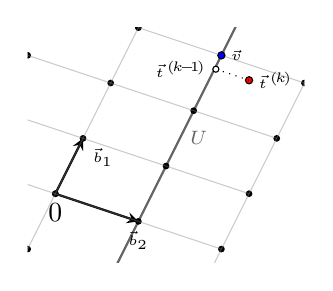
\begin{tikzpicture}
		\clip (-10pt,-25pt) rectangle (90pt, 60pt);
			%\draw[step=10pt,gray,opacity=0.1, very thin] (-40pt,-30pt) grid (100pt, 100pt);
			\foreach \y in {-2,...,5}
			\foreach \x in {-2,...,3}
			\filldraw(\x*40pt+\y*10pt, 10pt*\x+20pt*\y) circle (1pt);
			\filldraw(0pt,0pt) circle (1pt) node[below]{$0$};

			\draw[->, -stealth, black, thick] (0,0) -- (30pt, -10pt) node[font=\tiny, below]{$\bvec_2$};
			\draw[->, -stealth, black, thick] (0,0) -- (10pt, 20pt) node[font=\tiny, below right]{$\bvec_1$};
			\filldraw[fill=red](70pt, 41pt) circle (1.3pt) node[font=\tiny, right]{$\tvec^{(\mkern-2mu k \mkern-2mu)}$};
			%vertical lines:
			%\draw[gray, opacity=0.4] (-40pt, -10pt) -- (0pt, 70pt);
			\draw[gray, opacity=0.4] (-20pt, -40pt) -- (40pt, 80pt);
			\draw[black, thick, opacity=0.6] (20pt, -30pt) -- (70pt, 70pt) node[font=\scriptsize, midway, right]{$U$};
			\draw[gray, opacity=0.4] (50pt, -40pt) -- (90pt, 40pt);

			%horizontal lines:
			\draw[gray, opacity=0.4] (-30pt, 10pt) -- (60pt, -20pt);
			\draw[gray, opacity=0.4] (-20pt, 30pt) -- (70pt, 0pt);
			\draw[gray, opacity=0.4] (-40pt, 60pt) -- (80pt, 20pt);
			\draw[gray, opacity=0.4] (30pt, 60pt) -- (90pt, 40pt);
			%\draw[gray, opacity=0.4] (-50pt, -30pt) -- (70pt, 0pt);	
			
			%projection
			\draw[black, dotted] (70pt, 41pt) -- (58pt, 45pt);
			\filldraw[fill=white](58pt, 45pt) circle (1.1pt) node[font=\tiny, left] {$\tvec^{(\mkern-2mu k\mkern-3mu - \mkern-4mu 1 \mkern-2mu)}$};
			
			%solution
			\filldraw[fill=blue](60pt, 50pt) circle (1.3pt) node[font=\tiny, right]{$\vvec$};
	\end{tikzpicture}
	\caption{\scriptsize Babai's $\NP$ Algorithm on a `good' basis. The target point $t^{(k)}$ (red) is projected onto the closest hyperplane $U=\bvec_2+\Span(\bvec_1).$ The recursive call for this 1-dimensional $U$ projects $\tvec^{(k-1)}$ onto the closest zero-dimensional subspace, i.e.\ lattice point $\vvec$ (blue). }
                \label{fig:NP1}
	\end{subfigure}%
	~
    \begin{subfigure}[b]{0.32\textwidth}
    		\centering
    		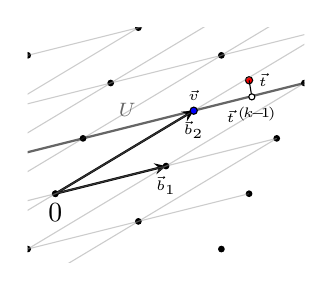
\begin{tikzpicture}
		\clip (-10pt,-25pt) rectangle (90pt, 60pt);
			\foreach \y in {-2,...,5}
			\foreach \x in {-2,...,3}
			\filldraw(\x*40pt+\y*10pt, 10pt*\x+20pt*\y) circle (1pt);
			\filldraw(0pt,0pt) circle (1pt) node[below]{ $0$};

			\draw[->, -stealth, black, thick] (0,0) -- (40pt, 10pt) node[font=\tiny, below]{$\bvec_1$};
			\draw[->, -stealth, black, thick] (0,0) -- (50pt, 30pt) node[font=\tiny, below]{$\bvec_2$};
			\filldraw[fill=red](70pt, 41pt) circle (1.3pt) node[font=\tiny, right]{$\tvec$};
			%vertical lines:
			\draw[gray, opacity=0.4] (-50pt, -30pt) -- (100pt, 60pt);
			\draw[gray, opacity=0.4] (-40pt, -10pt) -- (110pt, 80pt);
			\draw[gray, opacity=0.4] (-30pt, 10pt) -- (70pt, 70pt);
			\draw[gray, opacity=0.4] (-70pt, 0pt) -- (80pt, 90pt);
			\draw[gray, opacity=0.4] (-60pt, -50pt) -- (90pt, 40pt);
			\draw[gray, opacity=0.4] (-20pt, -40pt) -- (80pt, 20pt);
			
			%horizontal lines:
			\draw[gray, opacity=0.4] (-50pt, 40pt) -- (70pt, 70pt);
			\draw[gray, opacity=0.4] (-60pt, 20pt) -- (100pt, 60pt);
			\draw[black, thick, opacity=0.6] (-70pt, 0pt) -- (90pt, 40pt) node[font=\scriptsize, above, pos=0.6]{$U$};
			\draw[gray, opacity=0.4] (-40pt, -10pt) -- (80pt, 20pt);
			\draw[gray, opacity=0.4] (-50pt, -30pt) -- (70pt, 0pt);	
			
			%projection 
			\draw[black] (70pt, 41pt) -- (71pt, 35pt);
			\filldraw[fill=white](71pt, 35pt) circle (1.1pt) node[font=\tiny, below] {$\tvec^{(\mkern-2mu k\mkern-3mu - \mkern-4mu 1 \mkern-2mu)}$};
			
			%solution
			\filldraw[fill=blue](50pt, 30pt) circle (1.3pt) node[font=\tiny, left, above]{$\vvec$};
			
	\end{tikzpicture}
	\caption{\scriptsize Babai's $\NP$ Algorithm on a `bad' basis for the same lattice. Now the target point $\tvec^{(k)}$ (red) is projected onto the hyperplane $U=\bvec_2+\Span(\bvec_1)$ but for different $\bvec_2, \bvec_1$, so the hyperplane has changed. The returned vector $\vvec$  is not the closest vector.}
	\label{fig:NP2}
    \end{subfigure}%
    ~
    \begin{subfigure}[b]{0.32\textwidth}
    		\centering
    		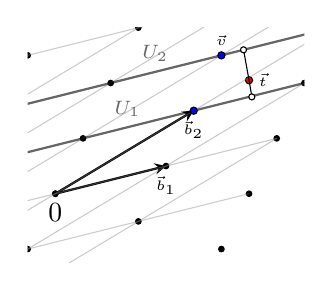
\begin{tikzpicture}
		\clip (-10pt,-25pt) rectangle (90pt, 60pt);
			%\draw[step=10pt,gray,opacity=0.1, very thin] (-40pt,-30pt) grid (100pt, 100pt);
			\foreach \y in {-2,...,5}
			\foreach \x in {-2,...,3}
			\filldraw(\x*40pt+\y*10pt, 10pt*\x+20pt*\y) circle (1pt);
			\filldraw(0pt,0pt) circle (1pt) node[below]{ $0$};

			\draw[->, black, -stealth, thick] (0,0) -- (40pt, 10pt) node[font=\tiny, below]{$\bvec_1$};
			\draw[->, black, -stealth, thick] (0,0) -- (50pt, 30pt) node[font=\tiny, below]{$\bvec_2$};
			\filldraw[fill=red](70pt, 41pt) circle (1.3pt) node[font=\tiny, right]{$\tvec$};
			%vertical lines:
			\draw[gray, opacity=0.4] (-50pt, -30pt) -- (100pt, 60pt);
			\draw[gray, opacity=0.4] (-40pt, -10pt) -- (110pt, 80pt);
			\draw[gray, opacity=0.4] (-30pt, 10pt) -- (70pt, 70pt);
			\draw[gray, opacity=0.4] (-70pt, 0pt) -- (80pt, 90pt);
			\draw[gray, opacity=0.4] (-60pt, -50pt) -- (90pt, 40pt);
			\draw[gray, opacity=0.4] (-20pt, -40pt) -- (80pt, 20pt);
			
			%horizontal lines:
			\draw[gray, opacity=0.4] (-50pt, 40pt) -- (70pt, 70pt);
			\draw[black, thick, opacity=0.6] (-60pt, 20pt) -- (100pt, 60pt) node[font=\scriptsize, above, pos=0.6]{$U_2$};
			\draw[black, thick, opacity=0.6] (-70pt, 0pt) -- (90pt, 40pt) node[font=\scriptsize, above, pos=0.6]{$U_1$};
			\draw[gray, opacity=0.4] (-40pt, -10pt) -- (80pt, 20pt);
			\draw[gray, opacity=0.4] (-50pt, -30pt) -- (70pt, 0pt);	
			
			%projections 
			\draw[black] (70pt, 41pt) -- (71pt, 35pt);
			\filldraw[fill=white](71pt, 35pt) circle (1.1pt);
			
			\draw[black] (70pt, 41pt) -- (68pt, 52pt);
			\filldraw[fill=white](68pt, 52pt) circle (1.1pt);
			
			%solutions
			\filldraw[fill=blue](50pt, 30pt) circle (1.3pt);
			\filldraw[fill=blue](60pt, 50pt) circle (1.3pt) node[font=\tiny, above]{$\vvec$};
	\end{tikzpicture}
	\caption{\scriptsize Lindner-Peikert $\NPs$ Algorithm on the same `bad' basis. We set $\dvec = (1, 2)$ and project the target $\tvec$ onto two hyperplanes $U_1 = \bvec_2+\Span(\bvec_1), U_2 = 2\bvec_2+\Span(\bvec_1)$. The output points are marked blue. The closets point $\vvec$ is found among them.}
	\label{fig:NP3}
    \end{subfigure}%
    \caption{$\NP$(\texttt{s}) Algorithms}
    \label{fig:NPAlgs}
\end{figure}

For Eq.~(\ref{eq:BabaiProof}) to be smaller than 0, which translates to a constant success probability for the Babai's \LWE decoding, the \BKZ parameter $\beta$ must be set almost as large as the lattice dimension $m$. For example, for parameters $q=\bigO(n^2), \alpha=\bigO(1/n^{3/2})$, Eq.~(\ref{eq:BabaiProof}) is smaller than 0 when $\beta > \frac{1}{2} \frac{m}{\ca - \tfrac{n}{m} \cq}$. Setting $m = 2 \frac{\cq}{\ca} n$ (as this choice minimizes $\beta$), yields $\beta > 2 \frac{\cq}{\ca^2}n \approx \frac{16}{9}n$. For such large $\beta$, the \BKZ reduction is not efficient. Choosing smaller $\beta$ and, hence, decreasing the running time of \BKZ reduction, leads to a super-exponentially small success probability of the decoding (case 1 in Thm.~\ref{thm:PsuccBabai}).

To amplify the success probability of Babai's algorithm (at the expense of its running time), Lindner and Peikert \cite{RSA:LinPei11} proposed an extended variant of the $\NP$ algorithm. Instead of choosing only one closest hyperplane $U_i$ (line \ref{algline:BabaiChoosePlane} in Alg.~\ref{alg:Babai}), we choose several, say $d$, close hyperplanes (line \ref{algline:LPChoosePlane} in Alg.~\ref{alg:LP}) and project the target vector onto them. This results in $d$ new targets which are, in turn, projected onto $d'$ several close hyperplanes (see Fig.~\ref{fig:NP3}). For example, Fig.~\ref{fig:TwoTreesLP} represents the case $m=3, \dvec = (3, 2, 1)$. Babai's $\NP$ algorithm corresponds to $\dvec = \vec{1}$.

Geometrically this idea amounts to stretching the search region $V_{\SubBabai} = \FP(\wBMat)$ to $V_{\SubLP} = \FP(\wBMat \cdot \DMat)$ for a diagonal matrix $\DMat$ having $(d_1, \ldots, d_m)$ on the main diagonal. In the end, we have $\prod_i d_i$ candidate error-vectors, out of which the shortest is chosen. 

The formal description of this algorithm, which we call the $\NPs$ algorithm, is given in Alg.~\ref{alg:LP}. In addition to a lattice and a target vector, the algorithm receives a vector $\dvec = (d_1, \ldots, d_m)$. Below we explain how to choose this vector.
%
% LP algorithm
%
\setlength{\intextsep}{\medskipamount}
\begin{algorithm}[h]
\caption{Lindner-Peikert $\NPs$ $(\BMat, \xvec, \protect \tvec, \dvec)$}
\label{alg:LP}
\textbf{Input:} $\BMat=(\bvec_1, \ldots, \bvec_m) \in \Z^{m \times m}, \xvec \in \Q^m, \tvec \in \xvec+\Span(\BMat), \evec' \in \Q^m$ \hfill \Comment $\evec'=\xvec=0$ in the initial call\\
\textbf{Output:} A set of pair $(\vvec, \evec')$ where $\vvec \in \Lat(\BMat)$ and $\evec' = \vvec - \tvec$
\begin{algorithmic}[1]
\State $\xvec^{(k)}\gets \xvec, \tvec^{(k)}\gets \tvec,\evec'^{(k)}\gets\evec'$. 
\State Let $\wBMat \gets \GSO(\BMat)$. 
\If {$k=0$} \Return $\{(\xvec,\evec') \}$
\EndIf
\State Compute $c^{(k)}_1 \gets \bigScProd{\tvec^{(k)}}{\frac{\wbvec_k}{\vphantom{\scalebox{1.6}x^2} \|\wbvec_k \|^2}}$
\State Compute $c^{(k)}_j = \bigScProd{\xvec^{(k)}}{\frac{\wbvec_k}{\vphantom{\scalebox{1.6}x^2} \|{\wbvec_k}\|^2}} + i^{(k)}_j$ for $i^{(k)}_j \in \Z, 1 \leq j \leq d_k$ s.t.\ $c^{(k)}_j$ are closest to $c^{(k)}_1$ \label{algline:LPChoosePlane}
	\For {\textbf{each} $(i^{(k)}_j, c^{(k)}_j)$} 
		\State $\xvec^{(k-1)}_j \gets \xvec^{(k)}+i^{(k)}_j \bvec_k$ \label{algline:LPChooseTranslate}
		\Comment $U_j^{(k-1)} = \xvec^{(k-1)}_j+\Lat(\BMat^{(k-1)})$ are the $d_k$ nearest planes
		\State $\evec'^{(k-1)}_j \gets \evec'^{(k)} + (c^{(k)}_1-c^{(k)}_j)\wbvec_k$ \label{algline:LPComputeError}
		\State $\tvec^{(k-1)}_j =\tvec^{(k)} - (c^{(k)}_1-c^{(k)}_j)\wbvec_k$ \label{algline:LPProjectTarget} \Comment Project onto $U_j^{(k-1)}$ 
\State \Return $\bigcup_j \NPs ((\bvec_1,\ldots,\bvec_{k-1}), \xvec^{(k-1)}_j,\tvec^{(k-1)}_j,\evec'^{(k-1)}_j, \dvec\mkern5mu)$
\EndFor
\end{algorithmic} 
\end{algorithm}

\paragraph{Analysis.} Like in the analysis of Babai's algorithm, we approximate the discrete Gaussian error $\evec$ sampled with parameter $\alpha q$ by a continuous one. Our goal is to determine a choice of $\dvec$ that guarantees a constant success probability and from such a choice, deduce the running time of the $\NPs$ algorithm. 

From \cite{RSA:LinPei11}, the success probability of the algorithm when applied to $m$ \LWE-samples is
\begin{equation} \label{eq:LPPSucc}
	\Psucc(\NPs) = \Pr[\evec \in \FP(\wBMat \DMat)] = \prod_{i=1}^{m} \Pr \Bigl[ | \ScProd{\evec}{\wbvec_i} | < \tfrac{d_i \| \wbvec_i \|^2}{2} \Bigr] = \prod_{i=1}^{m} \erf \Bigl( \tfrac{d_i \| \wbvec_i \|^2}{2 \alpha q} \Bigr),
\end{equation}
where $\erf = \frac{2}{\sqrt{\pi}} \int_0^x \exp(-t^2) \d t$. Tail-bounds on the Gaussian distribution (Eq.~(\ref{eq:TailBound})) suggest that if $\min_{1 \leq i \leq m} \frac{d_i \| \wbvec_i \|}{ \alpha q} = \smallo(1)$, then $\Psucc(\NPs) = \smallo(1)$. However, if $\min_{1 \leq i \leq m} \frac{d_i \| \wbvec_i \|}{ \alpha q} = \wLandau(\sqrt{\log m})$, then $\Psucc(\NPs) = 1 - \smallo(1)$.  Setting 
\begin{equation} \label{eq:dSeqLP}
	d_i = \Bigl\lceil \frac{\alpha q \cdot (\log m)^{c}}{ \| \wbvec_i \|} \Bigr\rceil
\end{equation}
for some constant $c > 1/2$, the decoding succeeds with probability almost 1. In case $\|\wbvec_1\| \gg \alpha q$ (which is the case for \LWE), we set the first $d_i$'s equal to $1$ and start increasing the sequence once $\| \wbvec_i \|$'s become equal or smaller than $\alpha q$. 

The recursive $\NPs$ Algorithm~\ref{alg:LP} has a tree-structure (see Fig.~\ref{fig:TwoTreesLP}) with the root corresponding to the initial call and every node is created by projecting the target onto one out of $d_i$ hyperplanes. As the result, each node on level $k$ has $d_{m-k+1}$ children. The superscripts for $\xvec^{(k)}, \evec'^{(k)}, \tvec^{(k)}$ denote the level, the root is on level $m$, the leaves are on level 0. Vectors $\xvec^{(k)}_j, \evec'^{(k)}_j, \tvec^{(k)}_j$ are the data associated to one node on level $k$, giving (1) a partial solution (w.r.t. the basis $\BMat$), (2) a partial error-vector (w.r.t. the basis $\wBMat$), and (3) a new target. 

Let $N_k$ be the number of nodes at level $k$ and $N$ be the total number of nodes. At the root we have $N_m = 1$. Down the tree, we have $N_k = \prod_{i=k+1}^m d_i$ and $N = \sum_{k=0}^m N_k$. The work done on a node is clearly polynomial in $m$, so the total complexity of Alg.~\ref{alg:LP} is $N \cdot \poly(m)$. The following theorem gives the value for $N$ when the $d_i$'s are set as in Eq.~(\ref{eq:dSeqLP}).

\begin{thm}[Analysis of the $\NPs$ Algorithm~\ref{alg:LP}] \label{thm:LPRunTime}
	Given a $\beta = \TLandau(n)$-\BKZ reduced basis that arises from $m = \TLandau(n)$ \LWE-samples with parameters $(n, q=\bigO(n^{\cq}), \alpha = \bigO(1 / n^{\ca}) )$ for positive constants $\cq >\ca$, the $\NPs$ Algorithm~\ref{alg:LP} with the $\dvec$ set as in Eq.~(\ref{eq:dSeqLP}), solves the Search-\LWE problem with success probability $1-\smallo(1)$ in time
	\begin{equation*}
T(\NP)=\poly(m) \cdot N = \begin{cases}
                  2^{\frac{1}{2} \bigl(\frac{m}{2\beta}-\ca + \frac{n}{m} \cq  \bigr)^2 (1+\smallo(1)) \cdot \beta\log\beta},			      \quad & \text{if }  \frac{m}{2 \beta} - \ca + \frac{n}{m} \cq  > 0  \\
                  \poly(m)                                     \quad&\text{if } \frac{m}{2 \beta} - \ca + \frac{n}{m}\cq  < 0,
                  \end{cases}
	\end{equation*}
and $\poly(m)$ memory (using depth-first search) assuming the Geometric Series Assumption holds and the \LWE error follows a continuous Gaussian distribution.
\end{thm}

\begin{proof}
	As in Thm.~\ref{thm:PsuccBabai}, under GSA, the inequality $\frac{m}{2 \beta} - \ca + \frac{n}{m}\cq  < 0$ translates into $\| \wbvec_m \| > \alpha q \cdot \poly(n)$. It immediately gives $d_i = \lceil \frac{\alpha q \cdot (\log m)^{c}}{ \alpha q \cdot \poly(n)} \rceil = 1$ (for some constant $c>1/2$ ). This is exactly Babai's $\NP$ algorithm which has $\poly(m)$ running time.
	
	In case $\frac{m}{2 \beta} - \ca + \frac{n}{m}\cq  > 0$, we have to increase some $d_i$'s to guarantee the desired success probability. Again as in Thm.~\ref{thm:PsuccBabai}, there exist a critical level $k^*$ s.t.\ $\| \wbvec_{k^*}\| > \alpha q$ and $k^*$ is maximal. This level is determined in Eq.~(\ref{eq:BabaiProof}) and we have $d_{k^{*}+1}>1$, i.e.\ we increase the $d_i$'s from this level. Since $N < (m+1) N_0$ (i.e.\ the total number of nodes is essentially determined by the number of leaves), the running time of Alg.~\ref{alg:LP} is given by (up to $\poly(m)$ factors) $N_0 = \prod_{i=1}^m d_i$. We have
	\begin{align*}
		N_0 = \prod_{i=1}^m d_i = 
		\prod_{i=1}^m \Bigl\lceil \frac{\alpha q \cdot (\log m)^{c}}{ \| \wbvec_i \|} \Bigr\rceil < 
		(1+(\log m)^c)^m \cdot \prod_{i=1}^{k^*} \Bigl\lceil \frac{\alpha q}{ \| \wbvec_i \|} \Bigr\rceil \prod_{i=k^*+1}^{m} \Bigl\lceil \frac{\alpha q}{ \| \wbvec_i \|} \Bigr\rceil \\
	\leq (1+\log{m}^c)^m 2^{m-k^*} \cdot \prod_{i=k^*}^{m} \Bigl\lceil \frac{\alpha q}{ \| \wbvec_i \|} \Bigr\rceil =
	(1+\log{m}^c)^m 2^{m-k^*} \cdot 2^{\bigl( \frac{(m-k^*)^2}{2 \beta^2} +\smallo(1) \bigr) \beta \log \beta},
	\end{align*} 
where the last product $\prod_{i=k^*+1}^{m} \bigl\lceil \frac{\alpha q}{ \| \wbvec_i \|)} \bigr\rceil$ was already computed in Lemma~\ref{lem:BabaiHelpingLemma} and Thm.~\ref{thm:PsuccBabai}. The factor $(1+\log{m}^c)^m 2^{m-k^*} = 2^{\bigO(m \log \log m)}$ contributes to the $\smallo(1)$-term in the theorem statement.
\end{proof}
The following corollary follows immediately from Thms.~\ref{thm:PsuccBabai} and \ref{thm:LPRunTime}.

\begin{corollary} \label{cor:BabaiAndLP}
	Given a $\beta = \TLandau(n)$-\BKZ reduced basis that arises from $m = \TLandau(n)$ \LWE-samples with parameters $(n, q=\bigO(n^{\cq}), \alpha = \bigO(1 / n^{\ca}) )$ for positive constants $\cq >\ca$, the decoding algorithms $\ENUM \in \{ \text{Babai's } \NP, \text{ Lindner-Peikert's } \NPs \text{ with } \dvec \text{ set as in Eq.~(\ref{eq:dSeqLP})}\}$ attain the running time/success probability trade-off
	\[
		\rho(\ENUM) = \frac{T(\ENUM)}{\Psucc(\ENUM)} = \begin{cases}
                  2^{\frac{1}{2} \bigl(\frac{m}{2\beta}-\ca + \frac{n}{m} \cq  \bigr)^2 (1+\smallo(1)) \cdot \beta\log\beta},			      \quad & \text{if }  \frac{m}{2 \beta} - \ca + \frac{n}{m} \cq  > 0  \\
                  \poly(m)                                     \quad&\text{if } \frac{m}{2 \beta} - \ca + \frac{n}{m}\cq  < 0,
                  \end{cases}
	\]
assuming the Geometric Series Assumption holds and the \LWE error follows a continuous Gaussian distribution.
\end{corollary}


\subsection{Generalized Pruning Algorithm} \label{sec:GenPrun}

\begin{figure}
  \begin{subfigure}[t]{0.42\textwidth}
  \centering
  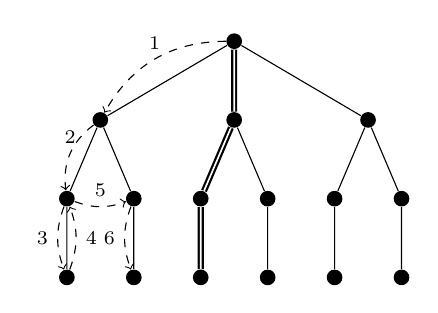
\begin{tikzpicture}[
    state/.style={circle, fill=black, inner sep=2pt},
    level distance=1.0cm,
    level/.style={sibling distance=17mm/#1}
]
\node [state] (a) {}
    child {node [state](b) {}
        child {node [state](c) {}
            child {node [state](d) {}}
            }
            child {node [state] (e) {}
            child {node [state] (f) {}}
            }
    }
    child {node [state](b1) {}
        child {node [state](b2) {}
            %child {node [state] {}}
            child {node [state](b3) {}}
            }
            child {node [state] {}
            child {node [state] {}}
            }
    }
    child {node [state] {}
        child {node [state] {}
            child {node [state] {}}
            }
            child {node [state] {}
            child {node [state] {}}
            }
    };
    \draw[->, dashed] (a) to [bend right=30] node [midway, above] {\scriptsize $1$} (b);
    \draw[->, dashed] (b) to [bend right=30] node [midway, above] {\scriptsize $2$} (c);
    \draw[->, dashed] (c) to [bend right=20] node [midway, left] {\scriptsize $3$} (d);
    \draw[->, dashed] (d) to [bend left=-20] node [midway, right] {\scriptsize $4$} (c);
    \draw[->, dashed] (c) to [bend right=20] node [midway, above] {\scriptsize $5$} (e);
    \draw[->, dashed] (e) to [bend right=20] node [midway, left] {\scriptsize $6$} (f);

    \draw[thick, double] (a) -- (b1);
    \draw[thick, double] (b1) -- (b2);
    \draw[thick, double] (b2) -- (b3);
\end{tikzpicture}%
\caption{\scriptsize Enumeration tree of the Lindner-Peikert algorithm for $3$-dimensional lattice with $\dvec = (3, 2, 1)$. }
\label{fig:TwoTreesLP}
\end{subfigure}
\hspace{10pt}
\begin{subfigure}[t]{0.47\textwidth}
\centering
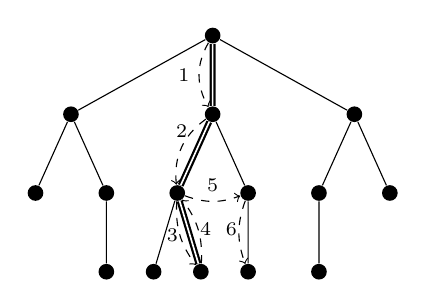
\begin{tikzpicture}[
    state/.style={circle, fill=black, inner sep=2pt},
    level distance=1.0cm,
    level/.style={sibling distance=18mm/#1}
]
\node [state] (a) {}
    child {node [state](b) {}
    	child {node [state] {} }
        child {node [state](c) {}
            child {node [state](d) {}}
            }
    }
    child {node [state](b1) {}
        child {node [state](b2) {}
            child {node [state] {}}
            child {node [state](b3) {}}
            }
            child {node [state](j) {}
            child {node [state](h) {}}
            }
    }
    child {node [state] {}
        child {node [state] {}
            child {node [state] {}}
            }
        child {node [state] {}}
    };
    \draw[->, dashed] (a) to [bend right=30] node [midway, left] {\scriptsize $1$} (b1);
    \draw[->, dashed] (b1) to [bend right=30] node [midway, above] {\scriptsize $2$} (b2);
    \draw[->, dashed] (b2) to [bend right=20] node [left, xshift=1mm] {\scriptsize $3$} (b3);
    \draw[->, dashed] (b3) to [bend left=-20] node [right, xshift=-1mm] {\scriptsize $4$} (b2);
    \draw[->, dashed] (b2) to [bend right=20] node [midway, above] {\scriptsize $5$} (j);
    \draw[->, dashed] (j) to [bend right=20] node [left, yshift=.4mm, xshift=1mm] {\scriptsize $6$} (h);

    \draw[thick, double] (a) -- (b1);
    \draw[thick, double] (b1) -- (b2);
    \draw[thick, double] (b2) -- (b3);
\end{tikzpicture}
\caption{\scriptsize Enumeration tree of the Generalized Pruning algorithm realized via some bounding function $\B$. As opposed to the left figure, the number of children varies for nodes on the same level.}
\label{fig:TwoTreesPrun}
\end{subfigure}
    \caption[Enumeration trees]{\footnotesize Enumeration tree of the Lindner-Peikert Algorithm (left) and the Generalized Pruning (right). The roots correspond to the initial call, the leaves contain the candidate error-vectors and the corresponding lattice vectors. The double-line represents the path (i.e.\ the choices of hyperplanes) that would have been chosen by the Babai's $\NP$ Alg.~\ref{alg:Babai}. The dashed curved arrows show the order of tree-traversals. On the left, the left-most child is visited first (usual depth-first tree-traversal). On the right, the `best' (w.r.t.\ the error-length)  child is chosen first (the \emph{best-first} traversal). 
    }
\label{fig:EnumTrees}
\end{figure}

\paragraph{Spherical and Linear-Length Pruning.} 

Note that the error-vector $\evec' = \sum_i e_i' \frac{\wbvec_i}{ \| \wbvec_i \|}$ is not explicitly bounded during the Lindner-Peikert's enumeration. 
It is done implicitly via restricting its individual coordinates $e_i'$. Each coordinate $e_i'$ is obtained by going one level down the enumeration tree: on level $k$ we compute $\evec'^{(k)} = \sum_{i=k+1}^m e_i' \frac{\wbvec_i}{ \| \wbvec_i \|}$ by adding $e'_{k+1}\frac{\wbvec_i}{ \| \wbvec_i \|}$ to $\evec'^{(k+1)}$ for an appropriately chosen coordinate $e'_{k+1}$ (see line \ref{algline:LPComputeError} in Alg.~\ref{alg:LP}).
By the end of the enumeration, $\evec'^{(k)}$ builds a final output $\evec'$ and hence, this final $\evec'$ will have length greater than $\| \evec'^{(k)} \|$. 
A moment's thought reveals that it is reasonable to make the number of children for a node dependent on the length of the error $\| \evec'^{(k)} \|$ associated to this node: the smaller this length is, the more children we want this node to have as it is more likely to lead to the correct solution, while if $\| \evec'^{(k)} \| \gg \sqrt{m} \alpha q$ (i.e.\ the accumulated error-length exceeds the expected length of the \LWE error), we might as well choose no children at all and stop the recursion for this node. This is why we use the term `pruning' as we prune the enumeration tree at some unpromising nodes.

For example, the \emph{Spherical Pruning} (\cite{SchE94}) chooses the number of the children for a $k\th$-level node with $\|\evec'^{(k)} \|^2 = \sum_{i=k+1}^m e_i'^2$ as $\TLandau  \left( \frac{1}{\| \wbvec_k \|^2} ( m (\alpha q)^2 - \sum_{i=k+1}^m e_i'^2) \right)$. This choice exactly captures our intuition: the shorter the accumulated error, the more children a node is allowed to have. We divide by $ \| \wbvec_k \|^2$ to get the actual number of the hyperplanes we recurse on (i.e.\ the number of children). It is easy to see that a pruning strategy enumerates all possible error-vectors that lie within the ball $\Ball(\tvec, \alpha q)$. 

Another pruning strategy, the \emph{Linear-Length Pruning} (\cite{EC:GamNguReg10}), reduces the search space of the Spherical Pruning by allowing a $k\th$-level error-vector to have norm $\| \evec'^{(k)} \|^2 \leq \TLandau( (m-k+1) (\alpha q)^2)$. This upper bound is the expected length of an $(m-k+1)$-dimensional vector with Gaussian entries of width $\alpha q$. It results, as in case of the Spherical Pruning, in the output error-vectors having norm $\TLandau(m \sqrt{\alpha q})$, but it is more restrictive on the intermediate levels.

There are several other pruning strategies considered in \cite{EC:GamNguReg10}, all aiming at reducing the search space by pruning the enumeration tree more aggressively, thus reducing the running time but sacrificing success probability (and hence, they are called \emph{Extreme Pruning} with the most `extreme' case being Babai's $\NP$). 
\vspace{10pt} %
\paragraph{Generalized Pruning.} All the enumeration strategies considered here can be described via a family of bounding functions $\B^{(k)}: \Q_{\geq 0}^{m-k} \rightarrow \Q_{\geq 0}$, $1 \leq k \leq m$. In general, this function may not even be efficiently computable in practice. For example, Aono in \cite{Ao14} suggests a way to find an optimal $\B^{(k)}$ given the Gram-Schmidt basis $\wBMat$ via solving an $m$-dimensional optimization problem. But for our $\GenPrun$ algorithm (Alg.~\ref{alg:GenPrun}) and its analysis we assume an efficiently computable family $\B^{(k)}$ which is given as an additional input.

%
% Generalized Pruning
%
\begin{algorithm}[t]
\caption{Generalized Pruning Algorithm $\GenPrun(\BMat, \protect \xvec, \protect \tvec, \protect \evec', \B^{(k)})$}
\label{alg:GenPrun}
\textbf{Input:} $\BMat=(\bvec_1, \ldots, \bvec_m) \in \Z^{m \times m}, \xvec\in\Q^m, \tvec \in \xvec+\Span(\BMat), \evec'\in\Q^m, \B^{(k)}$ \hfill ($\evec'=\xvec=0$ in the initial call)\\
\textbf{Output:} A set of pairs $(\vvec,\evec')$ with $\vvec\in \xvec+\Lat(\BMat)$ and $\evec' = \tvec-\vvec$ corresponding error vector
%\vspace{8pt}
\begin{algorithmic}[1]
\State $\xvec^{(k)}\gets \xvec, \tvec^{(k)}\gets \tvec,\evec'^{(k)}\gets\evec'$ 
\State Let $\wBMat\gets\GSO(\BMat)$
\If {$k=0$} \Return $\{(\xvec,\evec')\}$ \EndIf
\State Compute $c^{(k)}_1 \gets \bigScProd{\tvec^{(k)}}{\frac{\wbvec_k}{ \vphantom{\scalebox{1.6}x^2} \|\wbvec_k \|^2  }}$
\State
Let $e'_i = \ScProd{\evec'^{(k)}}{\frac{\wbvec_i}{\vphantom{\scalebox{1.6}x^2} \|\wbvec_i\|}}$ for $k< i \le m$ \Comment Coefficients of $\evec'$
\State Let $\Dmax^2 = \B^{(k)}(e'^2_m,\ldots,e'^2_{k+1})$ \Comment bound on distance of next hyperplanes \label{algline:GenPrunDmax}
\State Compute $c^{(k)}_j = \bigScProd{\xvec^{(k)}}{\frac{\wbvec_k}{\|{\wbvec_k}\|^2}} + i^{(k)}_j$ for all $i^{(k)}_j \in \Z$ s.t.\
$\abs{c_1^{(k)} - c_j^{(k)}}^2 \cdot \|\wbvec_k \|^2 \leq \Dmax^2$ \label{algline:GenPrunChoosePlane}
\For {\textbf{each} $(i^{(k)}_j, c^{(k)}_j)$} 
		\State $\xvec^{(k-1)}_j \gets \xvec^{(k)}+i^{(k)}_j \bvec_k$ \label{algline:GenPrunChooseTranslate}
		\Comment $U_j^{(k-1)} = \xvec^{(k-1)}_j+\Lat(\BMat^{(k-1)})$ are the nearby planes
		\State $\evec'^{(k-1)}_j \gets \evec'^{(k)} + (c^{(k)}_1-c^{(k)}_j)\wbvec_k$
		\State $\tvec^{(k-1)}_j =\tvec^{(k)} - (c^{(k)}_1-c^{(k)}_j)\wbvec_k$ \Comment Project onto $U_j^{(k-1)}$ 
\State \Return $\bigcup_j \GenPrun ((\bvec_1,\ldots,\bvec_{k-1}), \xvec^{(k-1)}_j,\tvec^{(k-1)}_j,\evec'^{(k-1)}_j, \B^{(k)})$
\EndFor
\end{algorithmic} 
\end{algorithm}

The algorithm computes the maximal allowed distance (denoted $\Dmax$) to the next hyperplanes (line \ref{algline:GenPrunDmax} of Alg.~\ref{alg:GenPrun}) and chooses only the hyperplanes for which $e'^2_k$ satisfies $e'^2_k < \B^{(k)} (e'^2_m, \ldots, e'^2_{k+1}) = \Dmax^2$. The search region of \GenPrun is
\begin{equation*} 
	V_{\GP} = \Bigl\{ \evec' = \sum_k e'_k \frac{\wbvec_k }{\| \wbvec_k \| } \colon e_k^2 \leq \B^{(k)}(e'^2_m, \ldots, e'^2_{k+1}) \; \forall k \Bigr\}.	
\end{equation*}

The algorithm successfully solves the \LWE problem if the \LWE error-vector $\evec$ is contained in the search region $V_{\GP}$. It is easy to see that Generalized Pruning captures all the enumeration strategies discussed here. Namely,

\begin{itemize}
	\item $\B^{(k)}(e'^2_m, \ldots, e'^2_{k+1}) = \left( \frac{\| \wbvec_k \|}{2} \right)^2 $: Babai's $\NP$
	\item $\B^{(k)}(e'^2_m, \ldots, e'^2_{k+1}) = \left( \frac{d_k \| \wbvec_k \|}{2} \right)^2 $: Lindner-Peikert's $\NPs$
	\item $\B^{(k)}(e'^2_m, \ldots, e'^2_{k+1}) = \TLandau(m (\alpha q)^2) - \sum_{i=k+1}^m e'^2_i$: Spherical Pruning
	\item $\B^{(k)}(e'^2_m, \ldots, e'^2_{k+1}) = \TLandau( (m-k)(\alpha q)^2) - \sum_{i=k+1}^m e'^2_i $: Linear Pruning
	\item $\B^{(k)}(e'^2_m, \ldots, e'^2_{k+1}) = R_k^2 -  \sum_{i=k+1}^m e'^2_i$: pruned strategy with some level-dependent bounds $R_k$.  
\end{itemize}
 
All the extreme pruning approaches of \cite{EC:GamNguReg10} as well any numerically optimized strategy are covered by the last choice of $\B^{(k)}$.

For the analysis, we extend $\B^{(k)}$ to real-valued arguments so that we can apply the algorithm to a continuous Gaussian.

\paragraph{Analysis.} As before, we are interested in the ratio $\rho(\GP) = \frac{T(\GP)}{\Psucc(\GP)}$ ($\GP$ is used as a shorthand for Generalized Pruning). A family of bounding functions $\B^{(k)}$ defines the search region on level $k$ as
\begin{equation}\label{eq:VGP}
	V_{\GP}(k) =  \Bigl\{ \evec' = \sum_{i=k+1}^m e'_i \frac{\wbvec_i }{\| \wbvec_i \| } \colon e_j^2 \leq \B^{(j)}(e'^2_m, \ldots, e'^2_{j+1}) \;  k < j \leq m \Bigr\}.
\end{equation}

Let $N_k$ be the number of nodes at level $k$ and $p_k$ be the probability that the correct solution is retained on level $k$ (i.e.\ there exists a node with $\evec^{(k)}$ that can be extended to the correct \LWE error $\evec$ by traversing the tree down to the last level). We define a \emph{reasonable pruning} via requiring a set of conditions to be met by $\B^{(k)}, N_k,  p_k$. We assume that the error we seek for, follows a continuous Gaussian with parameter $\alpha q$ and that $ \| \wbvec_m \| < \alpha q < \| \wbvec_1 \| $. The latter is satisfied by the choice of $\beta$.

\begin{definition}[Reasonable Pruning] \label{def:ReasonablePruning}
Let $k^*$ be the maximal level s.t.\ $\| \wbvec_{k^*} \| > \alpha q$. The Generalized Pruning algorithm with the associated $\B^{(k)}$ is \emph{reasonable} if the following conditions are satisfied
 \begin{enumerate}
 	\setlength\itemsep{0.1em}
 	\item $\B^{(k)}(e'^2_m, \ldots, e'^2_{k+1}) + \sum_{i=k+1}^m e'^2_i = \TLandau(m (\alpha q)^2)$ 
 	\item $\Psucc(\GP) \geq 2^{-\bigO(m)} \cdot p_{k^*}$
 	\item $N_k \leq 2^{\bigO(m)} \cdot N_{k^*}$ for $k \leq k^*$
 	\item $\frac{N_{k-1}}{N_k} = \WLandau(1)$ for $k \geq k^*$
 	\item $V_{\GP}(k^*)$ is convex.
 \end{enumerate}
\end{definition} 

Informally, the conditions in Def.~\ref{def:ReasonablePruning} have the following meaning: Condition 1 implies that we prune the nodes with the accumulated error larger than the expected length of the \LWE error. Conditions 2 and 3 mean that as soon as the correct error survived until the `critical' level $k^*$, we can find $\evec$ with high probability (Condition 2) at essentially no additional cost (Condition 3). For example, from $k^*$ down, we can start the Babai's $\NP$ algorithm. Condition 4 ensures that for levels above $k^*$ we choose \emph{at least} a constant number of hyperplanes (line \ref{algline:GenPrunChoosePlane} in Alg.~\ref{alg:GenPrun}) to recurse on. Note that on these upper levels we have $\| \wbvec_k \| < \alpha q$ for $k>k^*$, so we must have $\WLandau(1)$ hyperplanes at distance at most $\alpha q$.

We elaborate on the convexity condition a bit more. Let us take a closer look at the search region $V_{\GP}$. From the way the error-vectors $\evec'^{(k)}$ are constructed during the algorithm, the number of nodes at level $k$, denoted $N_k$, is the number of points in $V_{\GP}(k) - \evec$ that belong to the lattice $\Lat(\wbvec_m, \ldots, \wbvec_{k+1})$, i.e.\ to the orthogonal projection of $\Lat(\BMat)$ onto $\Span(\bvec_1, \ldots, \bvec_k)$ (the shift by $\evec$ does not change $N_k$ asymptotically but is needed for the proof below). The Gaussian Heuristic suggests that
\begin{equation*} %\label{eq:GaussHeuristic}
	N_k \approx \frac{\vol V_{\GP}(k)}{\prod_{i=k+1}^m \| \wbvec_i \|}.
\end{equation*}

We could use this approximation in our theorem below, but since it is enough in our setting to upper-bound $N_k$ up to a factor of $2^{\bigO(m)}$, we can prove the above equation by relying on a variant of Minkowski's Convex Body Theorem. 
Roughly, this theorem tells us that if an $m$-dimensional 0-symmetric convex point-set ($V_{\GP}(k)$ for us) has volume larger than the volume of a lattice, then it contains a non-zero point of this lattice. 

The generalization of this result is due to Rado \cite{R46}: instead of a 0-symmetric convex set, he considers a non-negative integrable function $f(\xvec)$  and connects the quantity $\sum_{\vvec \in \Lat} f(\vvec)$ with the value $\mathcal{V}(f) =~ \int_{- \infty < x_i < \infty} f(\xvec) \d \xvec$. The convexity condition of the set is replaced by the quasi-concavity condition for $f$: for a linear map ${\Lambda}$ from an $m$-dimensional vector space into itself, the function $f$ must satisfy $f(\Lambda \xvec - \Lambda \yvec) \geq \min \{ f(\xvec), f(\yvec) \}$.
Later in Thm.~\ref{thm:GenPrunRunTime}, we consider $\Lambda$ acting like $\Lambda \xvec = \tfrac{1}{2} \xvec$. 
Minkowski's Convex Body Theorem is a special case of the Thm.~\ref{thm:Rado} for $f(\xvec)$ being a characteristic function of a convex symmetric set $V$ in which case $\mathcal{V}(f) = \vol V$.

\begin{thm}[Rado's generalization of Minkowski's Convex Body Theorem] \label{thm:Rado}
Let $f(\xvec)$ be a non-negative integrable function with the property $f(\Lambda \xvec - \Lambda \yvec) \geq \min \{ f(\xvec), f(\yvec) \}$ for all $\xvec, \yvec \in \R^m$ and a linear map $\Lambda: \R^m \rightarrow \R^m$. Then
\begin{equation} \label{eq:RadosThm}
	f(\zerovec) + \tfrac{1}{2} \sum_{\zerovec \neq \vvec \in \Lat} f(\vvec) \geq \frac{\abs{\det \Lambda}}{\det (\Lat)} \mathcal{V}(f),
\end{equation}
for every lattice $\Lat$, where 
\[
\mathcal{V}(f) = \int\limits_{\substack{ - \infty < x_i < \infty \\ 1 \leq i \leq m }} f(\xvec) \d \xvec,
\] 
and $\det(\Lambda)$ is the determinant of the $m \times m$ matrix that defines the transformation $\Lambda$.
\end{thm}
Following the proof of the theorem (see the book of Cassels \cite[Chap.\ III]{Cas97} for a comprehensive proof) and setting $\Lambda \xvec = \tfrac{1}{2} \xvec$ (so $\abs{\det \Lambda} = 2^{-m}$), we observe that up to $2^{\bigO(m)}$ the inequality given in Eq.~\eqref{eq:RadosThm} is an equality, so in our proof we rely on the fact that
\begin{equation} \label{eq:RadoEq}
f(\zerovec) + \tfrac{1}{2} \sum_{\zerovec \neq \vvec \in \Lat} f(\vvec) = \frac{2^{\pm \bigO(m)}}{\det (\Lat)} \mathcal{V}(f).
\end{equation}

Now we have the tools to present the main theorem of this section \emph{without} relying on the Gaussian Heuristic. 
We apply Eq.~(\ref{eq:RadoEq}) to the function $f(\xvec) = \tfrac{1}{(\alpha q)^{k^*}} \int_{V_{\GP}(k^*)} \exp \left( \frac{-\pi \| \yvec \|^2}{(\alpha q)^2} \right) \d \yvec$ and to the lattice $\Lat(\wbvec_m, \ldots, \wbvec_{k^*+1})$, where $k^*$ is the `critical' level as in Def.~\ref{def:ReasonablePruning}. $f(\xvec)$ is the convolution of the Gaussian density function with the characteristic function of our convex search region $V_{\GP}(k^*)$ and hence, it satisfies the quasiconcavity condition of Thm.~\ref{thm:Rado}. 

\begin{thm}[Analysis of the $\GenPrun$ Algorithm~\ref{alg:GenPrun}] \label{thm:GenPrunRunTime}
Given a $\beta = \TLandau(n)$-\BKZ reduced basis that arises from $m = \TLandau(n)$ \LWE-samples with parameters $(n, q=\bigO(n^{\cq}), \alpha = \bigO(1 / n^{\ca}) )$ for positive constants $\cq >\ca$ s.t.\ $\frac{m}{2 \beta} + \frac{n}{m} \cq - \ca >0$, any reasonable (as in Def.~\ref{def:ReasonablePruning}) pruning algorithm $\GP$ has an expected (over the choice of $\evec$) running time/success probability trade-off
\[
	\rho(\GP) = \frac{\E[T(\GP)]}{\Psucc(\GP)} = 2^{\frac{1}{2} \bigl(\frac{m}{2\beta}-\ca + \frac{n}{m} \cq  \bigr)^2 (1+\smallo(1)) \cdot \beta\log\beta},
\]
with $\poly(m)$ memory (using depth-first search) assuming the Geometric Series Assumption holds and the \LWE error follows a continuous Gaussian distribution.
\end{thm}

\begin{proof}
	The amount of work done on one node of the enumeration tree of Alg.~\ref{alg:GenPrun} is clearly $\poly(m)$, so the total running time is $T(\GP) = \poly(m) \cdot \sum N_k$. For the `critical' level $k^*$ (i.e.\ maximal level with $\| \wbvec_{k^*} \| > \alpha q$), we have $N_i < 2^{\bigO(m)}$ for all $i$ (for $i<k^*$ due to Condition 3 in Def.~\ref{def:ReasonablePruning}, for $i>k^*$ by the definition of $N_k$). So for a reasonable pruning strategy, it holds that
	\[
		T(\GP) = 2^{\bigO(m)} N_{k^*}.
	\]
	As discussed above, $N_{k^*}$ is (up to $2^{\bigO(m)}$) the number of lattice vectors $\vvec \in \Lat (\wbvec_m, \ldots, \wbvec_{k^* +1})$ that lie in the convex region $V_{\GP} - \evec$. Taking the expectation over the choice of $\evec$, 
	\[
		\E_{\evec}[N_{k^*}] = \sum_{\vvec \in \Lat (\wbvec_m, \ldots, \wbvec_{k^* +1})} f(x) \qquad \text{where} \qquad f(\xvec) = \tfrac{1}{(\alpha q)^{k^*}} \int\limits_{V_{\GP}(k^*)} \exp \left( \frac{-\pi \| \yvec \|^2}{(\alpha q)^2} \right) \d \yvec.
	\]
	This expectation is essentially the left-hand side of Eq.~(\ref{eq:RadoEq}). Note that $f(x)$ is quasiconcave (as it is a convolution of two log-concave functions: the Gaussian density function and the characteristic function of the convex region $V_{\GP}$). For $\Lat = \Lat(\wbvec_m, \ldots, \wbvec_{k^* +1})$, we obtain
	\begin{align*}
			\E_{\evec}[N_{k^*}] &= \frac{2^{\pm \bigO(m)}}{\det (\Lat)} \int f(\xvec) \d \xvec = 
			\frac{2^{\pm \bigO(m)}}{\det (\Lat)} \int\limits_{V_{\GP}(k^*)} \int\limits_{\substack{ - \infty < y_i < \infty \\ 1 \leq i \leq m }} \frac{1}{(\alpha q)^{k^*}} \exp \left( \frac{-\pi \| \yvec \|^2}{(\alpha q)^2} \right) \d \yvec \d \xvec =  \\
			&= \frac{2^{\pm \bigO(m)} \vol V_{\GP}(k^*)}{\det (\Lat)}.  
	\end{align*}
	If the pruning is reasonable, we have $\Psucc(\GP) = 2^{-\bigO(m)} \cdot p_{k^*}$, where $p_{k^*}$ is the probability that there exist a vector in $V_{k^*}$ s.t.\ its $m-k^*$ coordinates extend to the \LWE error-vector, yielding
	\begin{align*}
		\frac{\E[T(\GP)]}{\Psucc(\GP)} &= \frac{2^{\pm \bigO(m)} \vol V_{\GP}(k^*)}{\det (\Lat) \cdot \tfrac{1}{(\alpha q)^{m-k^*}} \int\limits_{\xvec \in V_{\GP}(k^*)} \exp(- \tfrac{\pi \| \xvec \|^2}{(\alpha q)^2}) \d \xvec} = 
		\frac{2^{\pm \bigO(m)} \cdot (\alpha q)^{m-k^*} \vol V_{\GP}(k^*) }{\prod_{i=m-k^*}^m \| \wbvec_i \| \cdot \int\limits_{\xvec \in V_{\GP}(k^*)} \exp(- \tfrac{\pi \| \xvec \|^2}{(\alpha q)^2})} = \\
		&= \frac{2^{\pm \bigO(m)} \cdot (\alpha q)^{m-k^*} \int_{\xvec \in V_{\GP}(k^*)} 1 \d \xvec}{\prod_{i=m-k^*}^m \| \wbvec_i \| \cdot \int_{\xvec \in V_{\GP}(k^*)} 1 \d \xvec} = 
		2^{\frac{1}{2} \bigl(\frac{m}{2\beta}-\ca + \frac{n}{m} \cq  \bigr)^2 (1+\smallo(1)) \cdot \beta\log\beta},
	\end{align*} 
	where for the third equality we used Condition 1 in Def.~\ref{def:ReasonablePruning} stating that $e^{-\bigO(m)} \leq \exp(- \tfrac{\pi \| \xvec \|^2}{(\alpha q)^2}) \leq 1$ for any $\xvec \in V_{\GP}(k^*)$.
\end{proof}

We remark that for a pruning strategy that has $\Psucc \leq p_{k^*}$ and $T \geq \poly(m) N_{k^*}$, the result of Thm.~\ref{thm:GenPrunRunTime} gives a lower bound on the trade-off $\rho$ for such a strategy. 

Finally, note that the Lindner-Peikert $\NPs$ algorithm is a corner-case of a reasonable pruning: in the corners of the parallelepiped-shaped search region $V_{\NPs}$ Condition 1 is not satisfied. This is why we analyzed it separately. Now we can move on to the discussion on the total complexity of the \BDD attack on \LWE where we balance the running time of the reduction and enumeration phases.

\subsection{Total complexity of \LWE decoding} \label{sec:Balance}

The \BDD attack on \LWE is a two-phase algorithm: the enumeration (phase 2) in performed on a $\beta$-\BKZ reduced basis (phase 1). So far we have been discussing the second phase -- enumeration -- ignoring the complexity of the reduction. By now we have the quantity $\rho(\ENUM) = \frac{T(\ENUM)}{\Psucc(\ENUM)}$, and we can finally turn our attention to the total complexity of the attack taking into account the reduction: $\rho(\BDD) = \frac{T(\BKZ)+T(\ENUM)}{\Psucc(\ENUM)}$.

$T(\BKZ)$ is determined by the input parameter $\beta$ or, more precisely, by the running time of an \SVP-solver on a lattice of dimension $\beta$ (the dimension of the original lattice -- $m$ for \LWE -- only affects a polynomial factor in $T(\BKZ)$). We have already mentioned two ways to instantiate an \SVP-solver in Chap.~\ref{sec:PrelimLattices}:
	\begin{itemize}
		\item[--] $T(\BKZ) = 2^{\cBKZ \cdot \beta \log \beta + \smallo(\beta \log \beta) }$ with $\poly(\beta)$ space complexity due to Kannan \cite{STOC:Kannan83} for $\cBKZ = \TLandau(1)$ (Hanrot and Stehl\'{e} in \cite{C:HanSte07} estimate $\cBKZ = \tfrac{1}{2e}$),
		\item[--] $T(\BKZ) = 2^{\cBKZ \cdot \beta  + \smallo(\beta)}$ with $2^{\bigO(\beta)}$ memory due to Micciancio-Voulgaris \cite{STOC:MicVou10} and Aggarwal et al.\ \cite{STOC:ADRS15} (for the former, $\cBKZ = 2$, and for the latter $\cBKZ = 1$; the space complexity is $2^{\beta + \smallo(\beta)}$ for both algorithms).
	\end{itemize}  
	
From now on, we ignore the $\smallo(\cdot)$-terms in the exponents. The above two cases result into two statements for the complexity of the \BDD attack. We start with Kannan's \SVP. We make a distinction between enumerations that achieve a constant success probability (Lindner-Peikert $\NPs$, Spherical or Linear-Length Pruning) and those that have an arbitrarily small success probability (Babai's $\NP$, Extreme Pruning).
As in the previous sections, we assume the \LWE error follows a continuous Gaussian distribution with parameter $\alpha q$.
\begin{thm}[Super-exponential \BDD-attack on \LWE] \label{thm:BalanceSuperExp}
	The \LWE problem with parameters $(n, q=\bigO(n^{\cq})$, $\alpha = \bigO(1 / n^{\ca}) )$ where $\cq, \ca = \TLandau(1)$, can be solved via \BDD with (1) a $\beta=\TLandau(n)$-basis reduction running in time $2^{\cBKZ \beta \log \beta}$ and (2) any enumeration algorithm $\ENUM \in \{ \GenPrun, \NPs \}$ using the optimal choice of $m = \left( \frac{2 \cq}{\sqrt{2 \cBKZ}+\ca} + \smallo(1) \right) \cdot n$ samples in time 
\begin{align*}
		T(\BDD) = 2^{ \left( \cBKZ \cdot \frac{2 \cq}{(\sqrt{2 \cBKZ}+\ca)^2} \right) \cdot n \log n},
\end{align*}
	if $\Psucc(\ENUM) = 1 - \smallo(1)$. For arbitrary $\Psucc(\ENUM)$, the above quantity is a lower bound for $\rho(\BDD)$.
\end{thm}

\begin{proof}
	Assume we run an enumeration algorithm with $\Psucc(\ENUM) = 1 - \smallo(1)$. Investing more time in the reduction (i.e.\ improving the quality of the output basis) results in a faster enumeration, so the total running time $T(\BDD) = T(\BKZ)+ T(\ENUM)$ is minimized if the two phases are balanced. Thms.~\ref{thm:LPRunTime} resp.\ \ref{thm:GenPrunRunTime} give $T(\NPs)$ resp.\ $T(\GenPrun)$. On the logarithmic scale, the balancing condition $T(\BKZ) = T(\ENUM)$ is equivalent to (omitting the $\smallo(1)$-terms)
	\[
		\frac{1}{2} \left( \frac{m}{2 \beta} + \frac{n}{m} \cq - \ca \right)^2 \beta \log \beta = \cBKZ \beta \log \beta.
	\]
	This equation yields $\beta = \frac{1}{2} \frac{m}{\sqrt{2 \cBKZ}-(n/m)\cq + \ca}$. This expression attains its minimum at $m = \frac{2 \cq}{\sqrt{2 \cBKZ} + \ca}$, from where the first theorem statement easily follows. Note that for a constant success probability of enumeration, $\rho(\BDD) = \TLandau(T(\BDD))$.
	
	For arbitrary $\Psucc(\ENUM)$, we have $\rho(\BDD) = \frac{T(\BKZ)}{\Psucc(\ENUM)}+\rho(\ENUM) \geq T(\BKZ) + \rho(\ENUM)$, and we have just computed $T(\BKZ) + \rho(\ENUM)$. 
\end{proof}

Now we consider the case when a lattice-basis reduction has a \emph{single} exponential complexity $2^{\cBKZ \cdot \beta}$. Recall Thm.~\ref{thm:GenPrunRunTime} shows that for $\ENUM =  \GenPrun$, $\rho(\ENUM) = 2^{\TLandau(\beta \log \beta)}$. Cor.~\ref{cor:BabaiAndLP} states the same trade-off for the Babai's $\NP$ and Lindner-Piekert $\NPs$ algorithms.

So asymptotically, it is optimal to reduce the input basis to a point where the cost of enumeration switches from super-exponential to polynomial since in this case, $T(\BDD)$ is dominated by the reduction and stays singe-exponential. In the next theorem, we find a value of $\beta$ for which the reduction phase will produce a basis required for a $\poly(m)$-time enumeration that will produce the correct output with success probability almost 1. This enumeration may be either the Babai's $\NP$, Lindner-Peikert $\NPs$ or any (reasonable) pruning strategy with $\poly(m)$ number of nodes. 

\begin{thm}[Single-exponential \BDD-attack on \LWE] \label{thm:BalanceSingleExp}
	The \LWE problem with parameters ($n$,\linebreak $q=\bigO(n^{\cq})$, $\alpha = \bigO(1 / n^{\ca}) $) where $\cq, \ca = \TLandau(1)$ can be solved via \BDD with (1) a $\beta= \Bigl( \frac{2 \cq}{\ca^2} + \smallo(1) \Bigr) \cdot n$-basis reduction running in single-exponential time $2^{\cBKZ \beta}$ and (2) $poly(m)$-time enumeration algorithm using the optimal choice $m = \left( \frac{2 \cq}{\ca} + \smallo(1) \right) \cdot n$ of samples in time
	\[
		T(\BDD) = 2^{ \Bigl(\cBKZ \cdot \frac{2 \cq}{\ca^2} + \smallo(1) \Bigr) \cdot n}
	\]
	with $\Psucc(\BDD) = 1 - \smallo(1)$.
\end{thm}

\begin{proof}
 To guarantee a constant success probability and polynomial running time for enumeration, we need to ensure that the last Gram-Schmidt vector of the basis returned by $\beta$-reduction satisfies $\|  \wbvec_m\| > \alpha q$. This is equivalent to (cf.\ Cor.~\ref{cor:BabaiAndLP}) $\frac{m}{2 \beta} - \ca + \frac{n}{m}\cq  < 0$, so $\beta$ must be set as
 \[
 	\beta > \frac{1}{2} \frac{m}{\ca - \cq \cdot n/m}. 
 \]
 
 This value is minimized for $m = \frac{2 \cq}{\ca}$ yielding $\beta > \frac{2 \cq}{\ca^2} \cdot n$. The theorem statement follows directly from plugging this value in the running time of the reduction. 
\end{proof}

This theorem concludes the discussion on the two-phase \BDD attack on \LWE. In the following section, we briefly discuss some other lattice-based methods to solve \LWE.

\subsection{Other lattice-based algorithms for \LWE} \label{sec:OtherAttacks}

To provide a complete picture on lattice-based attacks, we briefly describe two other algorithms one can use to solve \LWE. First is the so-called Kannan's homogenization technique \cite{Kan87}, which allows us to convert a $\CVP$ (resp.\ $\BDD$) instance to an $\SVP$ (resp.\ $\uSVP$) instance in a higher-dimensional lattice (the approximation parameter $\gamma$ in $\uSVP$ depends on the promise given in the original \BDD instance). This approach is know as the \emph{embedding} technique. We show the running time of this attack when applied to $\LWE$ in Thm.~\ref{thm:Embed}. An analogous result was presented in \cite{APS15} but our choice of $m$ is different.

The second approach we consider, the so-called \emph{dual} attack, tackles the \emph{decisional}-\LWE (see Def.~\ref{def:decLWE}) by solving $\appSVP$ (for an appropriate choice of $\gamma$) in the lattice dual to the \LWE lattice. 

\paragraph{Embedding.} $\mkern-6mu$ Assume a \CVP instance $(\Lat(\BMat), \tvec)$ has a solution $\vvec \in \Lat(\BMat)$. Consider a higher-dimensional lattice $\LEmb (\BMat, \tvec)$ generated by the columns of the matrix
\begin{equation} \label{eq:BEmbed}
	\BMat' = \begin{pmatrix}
				\BMat & \tvec \\
				0 & \tau
			\end{pmatrix},
\end{equation}
 where $\tau$, known as the \emph{embedding factor}, is chosen such that the shortest vector in $\LEmb(\BMat, \tvec)$ is of the form $(\vvec, e)$ for $e \neq 0$. In other words, solving $\SVP$ on $\LEmb(\BMat, \tvec)$ leads to a solution of the original $\CVP$ problem. Note that $\tau$ should not be too small (in the worst-case $\CVP$ instance, $\tau$ is $\tfrac{1}{2} \lambda_1(\Lat(\BMat))$), otherwise the last column of the matrix $\BMat'$ may be used too often and the returned shortest vector may be the closest to a multiple of $\tvec$. On the other hand, $\tau$ should not be too large, otherwise the returned shortest vector will lie in $\Span(\BMat)$ giving no information on the solution to \CVP. 
 
 The embedding technique becomes more powerful if we know some information on the $\CVP$ instance we are given. In the $\BDD$ problem, for instance, we have a promise that the target vector is much closer to the solution-vector $\vvec$ than to any other lattice-vector. In this case, Kannan's technique leads us to the $\uSVP$ problem. In case of \LWE, we know that $\| \tvec - \vvec \| = \| \evec \| = \TLandau(\alpha q \sqrt{m})$, and, further, we know $\lambda_1(\BMat)$. It allows us to estimate $\lambda_1$ and $\lambda_2$ in $\LEmb(\BMat, \tvec)$ as $\lambda_1^2= \| \evec \|^2 + \tau^2$, $\lambda_2 = \lambda_1(\BMat)$, and hence, we know the gap of the lattice $\LEmb$. This gives us a bound on parameter $\gamma = \frac{\lambda_2}{\lambda_1}$ in the $\uSVP$ problem we are solving. 

We solve the $\uSVP$ problem via lattice-basis reduction. From Eq.~(\ref{eq:b1norm}), we know that an $m$-dimensional $\beta$-\BKZ reduced lattice, gives a $\beta^{\frac{m}{2 \beta}}$ approximation to a shortest vector of the lattice. Hence, as soon as the first (the shortest) vector of the reduced basis satisfies $\| \bvec_1 \| < \lambda_2(\LEmb(\BMat, \tvec))$, this vector is the shortest in $\LEmb(\BMat, \tvec)$ and, consequently, is the solution to $\uSVP$. All that remains is to determine the \BKZ parameter $\beta$ for which the first vector meets the requirement. 

In the theorem below, we consider the two possible running times of $\BKZ$, super-exponential (resp.\ single-exponential) as $f(\beta) = \beta \log \beta + \smallo(\beta \log \beta)$ (resp.\ $f(\beta) = \beta + \smallo(\beta)$). We omit the $\smallo(\cdot)$-terms. The space complexity of the attack is polynomial in the first case and exponential in $\beta$ in the second.
\begin{thm}[Complexity of the Embedding Attack on \LWE] \label{thm:Embed}
	The \LWE problem with parameters $(n, q=\bigO(n^{\cq}), \alpha = \bigO(1 / n^{\ca}) )$ where $\cq, \ca = \TLandau(1)$, can be solved via \emph{embedding} using a $\beta$-\BKZ reduction with $T(\BKZ) = 2^{\cBKZ \cdot f(\beta)}$, where either $f(\beta) = \beta$, or $f(\beta) = \beta \log \beta$ using the optimal choice of $m = \left( \frac{2 \cq}{\ca} + \smallo(1) \right) \cdot n$ of \LWE samples in time
	\[
		T(\Embed) = 2^{\left( \cBKZ \cdot \frac{2\cq}{\ca^2} + \smallo(1) \right) f(n)}.
	\]
\end{thm}

\begin{proof}
	Let $\BMat$ be a matrix that arises from $m$ \LWE samples and let $\LEmb(B, \tvec)$ be the corresponding $m+1$-dimensional lattice generated by the matrix defined in Eq.~(\ref{eq:BEmbed}). Let us estimate the first two successive minima $\lambda_1$, $\lambda_2$ for the embedded lattice. Setting the embedding factor $\tau = \TLandau(\| \evec \|)$, we obtain
	\[
		\lambda_1^2(\LEmb(\BMat, \tvec)) = \| \evec \|^2 + \tau^2 = \TLandau((\alpha q)^2 m).
	\]
	For a $q$-ary \LWE lattice, we have $\lambda_1(\Lat(\BMat)) =\min \{ q, \sqrt{m} q^{1 - n/m} \}$. For our choice of $m$, Minkowski's bound is always smaller, leading to
	\[
		\lambda_2(\LEmb(\BMat, \tvec)) = \lambda_1(\Lat(\BMat)) \leq \sqrt{m} q^{1 - n/m}.
	\] 
	The value of $\beta$, for which the $\beta$-reduced basis achieves an approximation of $\frac{\lambda_2(\LEmb(\BMat, \tvec))} { \lambda_1(\LEmb(\BMat, \tvec))}$, is given by
	\[
		\beta^{m / (2 \beta)} = \frac{\lambda_2(\LEmb(\BMat, \tvec))}{\lambda_1(\LEmb(\BMat, \tvec))} = \TLandau \left( \frac{q^{1-n/m}}{\alpha q} \right),
	\]
	assuming Minkowski's bound holds with equality. This is equivalent to $\beta = \left( \frac{2 \cq}{\ca^2} + \smallo(1) \right) \cdot n$. The minimum value for $\beta$ is attained at $m = \left( \frac{2 \cq}{\ca} + \smallo(1) \right) \cdot n$. 
\end{proof}

There is no surprise that the complexity of the embedding attack is exactly the same as the complexity of the two-phase \BDD attack with the single-exponential reduction followed by a polynomial-time enumeration (cf.\ Thm.~\ref{thm:BalanceSingleExp}). Both methods are, in fact, equivalent: performing a Babai-type (i.e.\ polynomial) enumeration on a reduced basis can be interpreted as embedding the target into the reduced basis and then size-reducing it (i.e.\ running \LLL). After such a procedure, the first vector reveals the closest vector.

\paragraph{Dual attack \hspace*{-8pt}}, originally considered in \cite{MicReg09} and further discussed in \cite{C:KirFou15}, solves the \emph{decisional}-\LWE. 

Given an \LWE instance $(\AMat, \tvec = \AMat\transpose \svec + \evec \bmod q) \in \Z_q^{n \times m} \times \Z_q^m$, instead of working with the lattice $\qLat(\AMat\transpose)$ (i.e.\ the image of $\AMat\transpose$) as we did so far, we make use of another $q$-ary $m$-dimensional lattice -- the kernel of $\AMat$:
\begin{align} \label{eq:DualLattice}
	\qLATTp (\AMat) = \{ \xvec \in \Z^m \colon \AMat \xvec = \zerovec \bmod q \}.
\end{align}
This lattice is the scaled dual to $\qLat(\AMat\transpose)$ with determinant $\det \qLATTp (\AMat) = q^n$ (the duality follows from the fact that $\qLATTp (\AMat) = q (\Lat(\AMat\transpose))^*$). A basis for this lattice can be easily formed from a (non-zero) matrix $\XMat$ that satisfies $\AMat \XMat = 0 \mod q$.

Assume we have found a short non-zero vector $\vvec \in \qLATTp (\AMat)$. Computing $w = \langle\vvec,\tvec\rangle \bmod q = \vvec^t (\AMat\transpose \svec + \evec ) \mod q = \ScProd{\vvec}{\evec} \bmod q$, we can distinguish whether $\evec$ is uniform or Gaussian. 
If $\evec$ is uniform, $w$ is also uniform, while if $\evec$ is Gaussian, $w = \sum_i v_i e_i$ is Gaussian with parameter $\alpha q \cdot \| \vvec \|$ (again, we assume the \LWE error follows a continuous Gaussian distribution). 
In the second case, the statistical distance between $w \bmod q$ and a uniform random variable $\bmod \ q$ or, a \emph{bias} of a continuous Gaussian with parameter $\alpha q \cdot \| \vvec \|$, is $\delta = 2^{-\bigO(\alpha^2 \| \vvec \|^2)}$. 
(To see this, we take a Fourier transform over $\Z_q$ of the Gaussian density function with standard deviation $\alpha q \| \vvec \|$ and evaluate at $1/q$). 
There exists an efficient distinguisher that has the advantage $\delta$ in deciding whether $w$ is uniform or Gaussian. 
For instance, [\cite{EC:DucTraVau15}, Lemma 10] shows that for Gaussian $w$ with standard deviation $s$ over $\Z_q$, $\E[\cos \bigl( \tfrac{2 \pi w}{q}\bigr)] \geq \frac{q}{\pi} \sin \left( \tfrac{\pi}{q}\right) e^{-2 \pi^2 s^2/q^2} $ (cf.\ line \ref{algline:decLWEDistinguish} in Alg.~\ref{alg:Dual}), while for a uniform $w \in \Z_q$, $\E[\cos \bigl( \tfrac{2 \pi w}{q}\bigr)] = 0$.

%
% DUAL algorithm
%
\setlength{\intextsep}{\medskipamount}
\begin{algorithm}[t]
\caption{ Dual attack on decisional-\LWE $\DUAL (\AMat, \protect \tvec, \eps)$}
\label{alg:Dual}
\textbf{Input:} $\AMat \in \Z^{m \times k}, \tvec \in \Z^m$ where  either (1) $\tvec = \AMat\transpose \svec + \evec \bmod q$ or (2) $\tvec$ is uniform from $\Z_q^m$  \\
\textbf{Output:} ``Yes'' if $\tvec = \AMat\transpose \svec + \evec \bmod q$, ``No'' otherwise.
\begin{algorithmic}[1]
	\State Compute $\XMat$ s.t.\ $\AMat \XMat = 0 \bmod q$ via Gaussian elimination
	\State $\BMat \gets$ $\beta$-\BKZ ($\qLat(\XMat)$) with $\beta = \left( \frac{2 \cq}{(1/2 + \ca)^2} + \smallo(1) \right) \cdot n$\Comment{
	\scriptsize
	Although we do not know $\ca$, we can approximate it by  \hspace*{9.1cm} trying several $\ca \in [0, \cq]$ in a binary-search manner} 
	\normalsize
	\If {$ \exists \vvec \in \Lat(\BMat)$ s.t.\ $\|\vvec \| =  \bigO(n^{1/2+\ca - \eps})$} 
		\normalsize
		\If {$\cos \left( \frac{ 2 \pi \langle{\vvec},{\tvec} \mkern3mu\rangle} {q} \right)> \frac{q}{\pi} \sin \left( \frac{\pi}{q}\right) e^{-2 \pi^2  \cdot n^{1-\eps}}$} \label{algline:decLWEDistinguish}
			\State \Return ``Yes''
		\Else
			\State \Return ``No''
		\EndIf
	\EndIf
\end{algorithmic} 
\end{algorithm}

To keep the bias $\delta = 2^{-\bigO(\alpha^2 \| \vvec \|^2)}$ sub-exponential, we must have $\| \vvec \| = \bigO(n^{1/2+\ca - \eps})$ for any $\eps>0$. The following lemma estimates the value for $\beta$ s.t.\ a $\beta$-\BKZ reduction (now on $\qLATTp (\AMat)$) outputs $\vvec$ of desired length. 

\begin{lemma}[Decisional \LWE under the $\DUAL$ attack] \label{lem:DecisionalLWE}
The \emph{decisional}-\LWE problem with parameters $(n,$ $q=\bigO(n^{\cq})$, $\alpha = \bigO(1 / n^{\ca}) )$ where $\cq, \ca = \TLandau(1)$, can be solved via running a $\beta$-\BKZ reduction on the \emph{dual} lattice defined as in Eq.~(\ref{eq:DualLattice}) with $T(\BKZ) = 2^{\cBKZ \cdot f(\beta)}$, where either $f(\beta) = \beta$, or $f(\beta) = \beta \log \beta$, using the optimal choice of $m = \left( \frac{2 \cq}{1/2 + \ca} + \smallo(1) \right) \cdot n$ of samples in time
	\[
		T(\DUAL) = 2^{\left( \cBKZ \cdot \frac{2\cq}{(1/2+\ca)^2} + \smallo(1) \right) f(n)}.
	\]
with $\Psucc(\DUAL) = 2^{-\bigO(n^{1-\eps})}$ for $\eps>0$.
\end{lemma}

\begin{proof}
	From Eq.~(\ref{eq:b1norm}), the shortest vector of a $\beta$-\BKZ reduced basis of $\qLATTp (\AMat)$ satisfies $\| \vvec \| =\bigO \Bigl(\beta^{\tfrac{m}{2 \beta}} q^{\tfrac{n}{m}}\Bigr)$. Since we want the bias $\delta = 2^{-\bigO(\alpha^2 \| \vvec \|^2)}$ remain sub-exponential, the length of $\vvec$ should additionally satisfy $\|\vvec \|= \bigO(n^{1/2+\ca - \eps})$. Letting $\eps \rightarrow 0$, we choose $\beta = \left( \frac{2 \cq}{(1/2 + \ca)^2} + \smallo(1) \right) \cdot n$ and $m = \left( \frac{2 \cq}{1/2 + \ca} + \smallo(1) \right) \cdot n$. The theorem follows after substituting this $\beta$ into the running time of $\BKZ$.
\end{proof}

One of the remarkable properties of \LWE is the equivalence between the \emph{decisional} and \emph{search} versions of the problem. While the direction decisional-\LWE $\leq$ search-\LWE is trivial, the reverse is not that immediate. But it was proved to be true in several papers starting with the original result of Regev \cite{STOC:Regev05} for prime $q = \poly(n)$ and later extended to exponentially large composite moduli \cite{EC:MicPei12}. 

Now assume we want to use this equivalence to turn the result of Lemma \ref{lem:DecisionalLWE} into an algorithm for the search-\LWE. Note that the search-to-decision reduction requires a decisional-\LWE oracle that returns the correct answer (i.e.\ given a pair ($\avec, t$), it decides whether it is uniform or follows an \LWE distribution) with success probability $1-\smallo(1)$. The advantage of the distinguisher from Alg.~\ref{alg:Dual} is only sub-exponential: $\delta = 2^{-\bigO(n^{1-\eps})}$. In order to boost the advantage to $1-\smallo(1)$, we have to repeat the algorithm $\poly(n) \delta^{-2}$ times on independent \LWE samples.\footnote{More precisely, if we have found $m = \poly(n) \delta^{-1}$ short enough vectors $\vvec_i \in \qLATTp (\AMat_i)$, in Alg.~\ref{alg:Dual} we rather compute $\tfrac{1}{m}\sum_i \cos \left( \frac{ 2 \pi \langle{\vvec_i},{\tvec_i}\rangle} {q} \right) $ and check if the result is large enough. The correctness follows from Chernoff bounds. Note that for uniform $\tvec_i$'s, the expected value of this sum is 0.} 

In case we have sub-exponentially many \LWE samples, the asymptotical complexity stated in Lemma~\ref{alg:Dual} also holds for the search-\LWE, as the additional sub-exponential term that comes from the search-to-decisional reduction is suppressed by the leading-order single/super-exponential term. 

In a more natural scenario, when the number of \LWE samples is limited to only $\poly(n)$, we can resort to the so-called amplification technique aimed at creating exponentially many `fresh looking' \LWE samples out of $\poly(n)$-many samples. This amplification -- originally considered for the combinatorial \BKW attack on \LWE \cite{DCC:ACFFP15} -- can also be applied to the $\DUAL$ attack to generate new samples. 

We now briefly describe how to generate many new samples and refer the reader for the complete proof to \cite{DCC:HKM}. Given an \LWE instance $(\AMat, \tvec) \in \Z_q^{n \times m} \times \Z_q^m$ with $m = \poly(n)$, we sample a discrete Gaussian $\xvec \in \Z_q^m$ with parameter $\eta = \WLandau(1)$ and output $(\AMat \xvec \bmod q, \ScProd{\tvec}{\xvec} \bmod q) \in \Z_q^n \times \Z_q$. This tuple serves as a new \LWE sample. 

 
The main challenge in the amplification process is to show that (1) the new $\avec' = \AMat \xvec \bmod q$ is uniformly distributed over $\Z_q^n$ and independent from the original samples, and (2) the new error $e'$ in $\ScProd{\tvec}{\xvec} \bmod q$ is independent from $a'$ conditioned on the original samples. For a wide enough Gaussian $\xvec$ (i.e.\ taking $\eta$ to be a large constant in case $m = \TLandau(n \log n)$, or even $\eta = \TLandau(n^{c_{\eta}})$ for small constant $c_{\eta}$ in case we have only $m = \TLandau(n)$ original samples), the amplification by $\xvec$ was shown to satisfy the above conditions, \cite{DCC:HKM}. 

Note that the width of the error in this new amplified \LWE samples gets increased from $\alpha q$ to $\sqrt{m} \alpha q$, thus adding $1/2$ to $\ca$ (in case $\eta = \TLandau(1)$). Combining amplification with the result obtained for the $\DUAL$ attack on decisional-\LWE in Lemma~\ref{lem:DecisionalLWE}, yields the following theorem. 

\begin{thm}[Search-\LWE under the $\DUAL$ attack] \label{thm:DualSearch} The \emph{search}-\LWE problem with parameters ($n$, $q=\bigO(n^{\cq})$, $\alpha = \bigO(1 / n^{\ca})$) where $\cq, \ca = \TLandau(1)$ and $m$ \LWE samples, can be solved via running $\beta$-\BKZ reduction on the \emph{dual} lattice defined in Eq.~(\ref{eq:DualLattice}) with $T(\BKZ) = 2^{\cBKZ \cdot f(\beta)}$, where either $f(\beta) = \beta$, or $f(\beta) = \beta \log \beta$, in time
\[
		T(\DUAL) = \begin{cases}
			2^{\left( \cBKZ \cdot \frac{2\cq}{(1/2+\ca)^2} + \smallo(1) \right) \cdot f(n)} \quad &  \text{if} \;\; m = 2^{\bigO(n)} \\
			2^{\left( \cBKZ \cdot \frac{2\cq}{\ca^2} + \smallo(1) \right) \cdot f(n)} \quad & \text{if} \;\; m = \WLandau(n \log n).
		\end{cases}
\]
with $\Psucc(\DUAL) = 1- \smallo(1)$.
\end{thm}

The memory complexity of the attack is determined by the $\beta$-\BKZ reduction. Note that we do not have to store all the $2^{\bigO(n)}$ \LWE samples required by the decision-to-search reduction, but rather access (or amplify) them once needed. 

%\clearpage

\subsection{Summary of the results} \label{subsec:Summary}

In this section we summarize all the above results into Table~\ref{table:compareTable} and Fig.~\ref{fig:LWEPlots}. To make the overview complete, we include the results on asymptotic analysis of \BKW algorithm \cite{DCC:ACFFP15, C:KirFou15, DCC:HKM} and the linearization attack by Arora-Ge \cite{ICALP:AroGe11}.

The most important part of the table is the middle-column showing the constants in the exponents of the algorithms' runtimes. These constants are functions of \LWE parameters $\cq, \ca = \TLandau(1)$ and the constant $\cBKZ$ -- the exponent of the running time of \SVP solver called within \BKZ.

The upper part of the table states the complexities of attacks when only $\poly(n)$ memory is available. Only lattice-based attacks are applicable in this setting. In this part of the table, running times of all the algorithms are of order $2^{\TLandau(n \log n)}$. The reader should not be confused with the exponential number of samples and polynomial memory for the \DUAL attack: as explained in Sect.~\ref{sec:OtherAttacks}, we do not have to store all the samples at once. Since for Kannan's enumeration we have the term  $\smash{\sqrt{2 \cBKZ} = \sqrt{1/e} \approx 0.42}$ in the denominator, \BKZ+\ENUM is faster than \DUAL or \Embed algorithms when the number of samples is limited. The \DUAL attack, however, is asymptotically faster with $2^{\TLandau(n)}$ samples: the additive term $\sfrac12$ is slightly larger than $0.42$.

In the lower part of the table, exponential space-complexity is allowed resulting in single-exponential running times for the attacks. In this case, \emph{all} lattice-based attacks ($\BKZ+\ENUM$, \DUAL, \Embed) have the \emph{same} constants provided we can access only $\poly(n)$ \LWE samples. Exponential memory complexity comes from the lattice-basis reduction. The \DUAL attack, unlike other \emph{lattice-based} algorithms, can profit from exponential number of samples: the constant gets improved by the additive term of $\sfrac12$. Since the \DUAL attack needs exponentially many samples, this $\sfrac12$ term vanishes when we have a limited number of samples, in which case we have to run the amplification process. Recall that as the result of the amplification, a `fresh' \LWE sample of the form $(\avec', t')$ is produced, where $(\avec' = \AMat \xvec \bmod q, t' = \ScProd{\tvec}{\xvec} \bmod q)$ for some constant-width Gaussian $\xvec \in \Z_q^m$. It is easy to verify that in case of $\TLandau(n\log n)$ samples, the noise-rate in $t'$ increases exactly by $\sfrac12$, thus making the whole attack slightly worse. 

In case the number of samples is only linear in $n$, i.e. $m = \cm n$ for some constant $\cm$, the amplification works only for certain range of parameters $\cm, \cq, \ca$. This is due to the fact that we amplify the samples with a Gaussian $\xvec$ of a \emph{non-constant} width of order $\TLandau(n^{a})$ for some $a=\TLandau(1)$. In case $\ca<1/2+\cq/\cm$, or in other words, the noise in the original samples is too large relative to the modulus $q$, the standard deviation of the amplified samples will become larger than $q$. We refer the reader to \cite[Lemma 10]{DCC:HKM} for the details.

The same situation happens for the combinatorial \BKW algorithms, since we can again use amplification to produce enough samples for the algorithm to work. As opposed to the \DUAL attack, \BKW works only with exponential memory at disposal as it has to store many samples at once. 
Further, note that the denominators of the exponents for lattice-based attacks and for \BKW are the same except they are squared for the former. As a consequence, as soon as $\ca$ (or $\ca+\sfrac12$ for $2^{\TLandau(n)}$ many samples) is greater than 1, lattice-based techniques will outperform \BKW. Essentially it means that lattice-based attacks are better for low-noise rates.

Yet this is not always the case if we compare lattice-based attacks with the recent improvement for the \BKW algorithm by Kirchner-Fouque \cite{C:KirFou15} and Guo et al.\ \cite{C:GuoJohSta15}, which we name $\BKW2$. Its constant $\bigl(\sfrac{1}{\cq} + 2\ln(\tfrac{\cq}{\cq-\ca})\bigr)$ (in case of $2^{\TLandau(n)}$ many samples) is always smaller than the constant $\frac{\cq}{\ca+1/2}$ of \BKW, but not necessarily smaller than the constant for the lattice-based attacks. It hugely depends on the value $\cBKZ$ that obviously impacts their complexity. How exactly these all constants compare with each other is illustrated in Fig.~\ref{fig:LWEPlots}.

  
In the upper figure we compare single-exponential attacks with \emph{polynomial} number of \LWE samples. If we order the algorithms relative to the value of their constant for the parameters $(\cq, \ca)$, differently coloured areas correspond to different orderings. Since the constants for lattice-based attacks heavily rely on the value $\cBKZ$, we distinguish the two cases: (1) $\cBKZ = 1$ (Aggarwal et al. \cite{STOC:ADRS15} provable instantiation of an \SVP solver), and (2) $\cBKZ = 0.292$ (heuristic \SVP algorithm from \cite{SODA:BDGL16}). The subscript in the name of lattice-based attack indicates which case is chosen.  

For example, the orange area marks the range of \LWE parameters $(\cq, \ca)$ where the $\BKZ+\ENUM$ attack with $\cBKZ = 0.292$ performs better than $\BKW2$. For small values of $\ca$, however, \BKW algorithms outperform lattice-based techniques. This is due to the fact that combinatorial attacks are more robust to large-noise instances (the smaller $\ca$, the larger Gaussian width $\alpha q = n^{\cq - \ca}$), while lattice-based algorithms seem to perform significantly worse for an increased error-rate. We note that in case of $\poly(n)$ samples, by \ENUM we mean all the lattice-based attacks as they have the same constant.

We present the same figure for the case of \emph{exponential} number of samples. Here we take only the \DUAL algorithm to compare with \BKW. Notice that the horizontal areas (blue at the top and pink at the bottom) get shifted by $1/2$ comparatively to the upper figure -- the gain we have in the exponents for $\BKW$ and $\DUAL$ algorithms once we have exponentially many samples.

In both figures, the area below the green line denotes the values of $\cq, \ca$ for which hardness reductions (both classical and quantum) hold. As an example, for parameters $(\cq=2, \ca = 0.5)$ -- the values chosen for the cryptosystem described in \cite{STOC:Regev05} -- we make the constants explicit. 

%
% Table
%

\renewcommand{\arraystretch}{1.7}
\begin{table}[h]
	\begin{center}
		\begin{tabular}{|p{6.3cm} |c | c |}   \hline
			\multicolumn{3}{|c|}{$\rho(\ALG) = \frac{T(\ALG)}{\Psucc(\ALG)},$ \; $M=\text{Space}$} \\ \thickline 
			\multirow{2}{5.49cm}{\centering \textbf{polynomial memory}}& \multicolumn{2}{c|}{\cellcolor{gray!10}{$M=\poly(n), T(\BKZ) = 2^{\cBKZ n \log n}$}} \\ \cline{2-3} 
			& $\log(\rho) / (n \log n)$ & \# Samples \\ \hline
			\multicolumn{3}{|c|}{\textsc{ Lattice-based algorithms}}\\ \hline
			$\BKZ+\ENUM$, where $\ENUM$ is: & \multirow{4}{*}{\raisebox{4.5ex}{$ \frac{2 \cBKZ \cdot \cq}{(\sqrt{2 \cBKZ}+\ca)^2}$}} &
			\multirow{4}{*}{\raisebox{4.5ex}{$\Theta(n)$}}  \\[-1.5ex] 
			-- Babai~(Sect.~\ref{sec:BabaisNP}) & &   \\[-1.5ex]
			-- Lindner-Peikert~(Sect.~\ref{sec:LPNP}) & & \\ [-1.5ex]
			-- \GenPrun~(Sect.~\ref{sec:GenPrun}) & & \\ \hline 
			\multirow{2}{*}{{$\Dual$ (Sect.~\ref{sec:OtherAttacks}, Thm.~\ref{thm:DualSearch})}} & $\frac{2 \cBKZ \cdot \cq}{ \vphantom{\scalebox{1.2}x^2} \ca ^2}  $  & $\Theta (n \log n)$ \\ \cline{2-3}
			& $\frac{2 \cBKZ \cdot \cq}{ ( \ca +1/2)^2 } $ &  $2^{\Theta(n)}$ \\ \hline
			Embedding~(Sect.~\ref{sec:OtherAttacks}, Thm.~\ref{thm:Embed}) &  $ \frac{2 \cBKZ \cdot \cq}{\vphantom{\scalebox{1.2}x^2} \ca^2} $ & $\Theta(n)$ \\[2pt] \thickline %\thicklines
			\multirow{2}{5.49cm}{\centering \textbf{exponential memory}}& \multicolumn{2}{c|}{\cellcolor{gray!10}{$M=2^{\Theta(n)}, T(\BKZ) = 2^{\cBKZ n}$}} \\ \cline{2-3}
			& $\log(\rho) / n$ & \# Samples \\ \hline
			%\multicolumn{3}{|c|}{\textsc{ Lattice-based algorithms}}\\ \hline
			$\BKZ+\ENUM$, where $\ENUM$ is: & \multirow{4}{*}{\raisebox{4.5ex}{$\frac{2 \cBKZ \cdot \cq}{\ca^2}$}} & \multirow{4}{*}{\raisebox{4.5ex}{$\Theta(n)$}}  \\[-1.5ex]
			-- Babai~(Sect.~\ref{sec:BabaisNP}) & &   \\ [-1.5ex]
			-- Lindner-Peikert~(Sect.~\ref{sec:LPNP}) & & \\ [-1.5ex]
			-- \GenPrun~(Sect.~\ref{sec:GenPrun}) & & \\ \hline 
			\multirow{3}{*}{$\Dual$ (Sect.~\ref{sec:OtherAttacks}, Thm.~\ref{thm:DualSearch}), \cite{DCC:HKM}} & $\frac{2 \cBKZ \cdot \cq}{ (\ca +1/2)^2 } $ &  $2^{\Theta(n)}$  \\[1pt] \cline{2-3}
			& $\frac{2 \cBKZ \cdot \cq}{\vphantom{\scalebox{1.2}x^2} \ca^2}  $  & $\Theta (n \log n)$ \\ \cline{2-3}
			& $\frac{2 \cBKZ \cdot \cq}{\vphantom{\scalebox{1.2}x^2} (\ca-\cq/\cm)^2}  $  & $(\cm+\smallo(1))n$ \\ \hline
			Embedding~(Sect.~\ref{sec:OtherAttacks}, Thm.~\ref{thm:Embed}) &  $ \frac{2 \cBKZ \cdot \cq}{\vphantom{\scalebox{1.2}x^2} \ca^2} $ & $\Theta(n)$ \\[2pt] \hline
			\multicolumn{3}{|c|}{\textsc{ Combinatorial algorithms}}\\ \hline
			\BKW  (\cite{DCC:ACFFP15}) & $\frac{1}{2} \frac{\cq}{\ca+1/2} $ & $2^{\Theta(n)}$ \\ \hline
			\multirow{2}{*}{\BKW (Thm.\ 8 in \cite{DCC:HKM})} & $\frac{1}{2} \frac{\cq}{ \ca} $ & $\Theta(n \log n)$ \\ \cline{2-3}
			& $\frac{1}{2} \frac{\cq}{ \ca-\cq/\cm} $ & $(\cm+\smallo(1)) n$ \\ \hline	
			\BKWKF (\cite{C:GuoJohSta15, C:KirFou15}) & $ \bigl(\sfrac{1}{\cq} + 2\ln(\tfrac{\cq}{\cq-\ca})\bigr)^{\scriptscriptstyle -1} $ & $2^{\Theta(n)}$ \\ \hline
			\multirow{2}{*}{\BKWKF (Thm.\ 8 in \cite{DCC:HKM})} & $ \bigl(2\ln(\tfrac{\cq}{\cq-\ca})\bigr)^{\scriptscriptstyle -1} $ & ${\Theta(n\log n)}$ \\ \cline{2-3}
			& $ \bigl(2\ln(\tfrac{\cq-\cq/(\cm-1)}{\cq-\ca})\bigr)^{\scriptscriptstyle -1} $ & $(\cm+\smallo(1)) n$ \\
			 \thickline
			Arora-Ge (\cite{APS15, ICALP:AroGe11}), $\cq-\ca < \sfrac12$ & \scriptsize{$ \omega \cdot (1-2\ca) \cdot  n^{2 \ca} \log^2(n)$} & $\bigO(2^{n^{\ca} \log^2 n})$ \\ \hline
			Arora-Ge (\cite{APS15, ICALP:AroGe11}), $\cq-\ca \geq \sfrac12$ & \scriptsize{$\omega \cdot (2 \ca-1) \cdot n \log(n)$} & $\bigO(2^{n \log n})$ \\ \hline
		\end{tabular} 
	\end{center}
	\caption[\LWE attacks: asymptotics]{Asymptotic comparison of algorithms for \LWE. We denote $q = \bigO(n^{\cq})$, $\alpha =  \bigO(1/n^{\ca})$ and $\cBKZ$ is the constant hidden in the run-time exponent of lattice-basis reduction. 
	In order to run the \BKW (resp. \BKW2) algorithm when only \emph{linear} number of samples is available, the \LWE parameters must satisfy $\ca>1/2+\cq/\cm $ (resp.\  $\ca>1/2+\cq/(\cm-1)$) and $\cq>\cq/\cm - 1/2$ (resp.\ $\cq>\cq/(\cm-1) - 1/2$).  Such constraints come from the amplification.
	For Arora-Ge, $2\leq \omega <3 $ is the linear algebra constant.}
	\label{table:compareTable}
\end{table}

%
% Figures
%

\definecolor{LightSkyBlue}{RGB}{135, 206, 250}
\definecolor{Orange}{RGB}{255, 165,0}
\definecolor{LightSalmon}{RGB}{255, 160, 122}
\definecolor{LeafGreen}{RGB}{34, 139,  34}


\begin{figure}[h]
		\begin{subfigure}[h]{0.99\textwidth}
		\centering
		\begin{tikzpicture}
				    \node[anchor=south west,inner sep=0] (image) at (0,0) {\includegraphics[width=0.60\textwidth]{Plots/Plots_SingleExp_PolySamples.png}};
				    \begin{scope}[x={(image.south east)},y={(image.north west)}]
				    	
				    	% Help lines: Comment out once finished % 
				   		%\draw[help lines,xstep=.1,ystep=.1] (0,0) grid (1,1);
				    	%\foreach \x in {0,1,...,9} { \node [anchor=north] at (\x/10,0) {0.\x}; }
				    	%\foreach \y in {0,1,...,9} { \node [anchor=east] at (0,\y/10) {0.\y}; }
				    	
				    	%\node[draw=none] at (0.45, 0.15) {\tiny $\BKW2 \leq \ENUM2 \leq \BKW \leq \ENUM$};
				    	%\node[draw=none, color=black] at (0.6, 0.52) {Quantum reduction};
				    
				    	\draw[fill=LightSkyBlue, opacity=0.9] (1.0, 0.6) rectangle (1.05, 0.65) node[yshift=-2ex, xshift=17ex]{$\ENUMH \leq \BKW2 \leq \ENUMOne \leq \BKW$};
				    	\draw[fill=Orange] (1.0, 0.5) rectangle (1.05, 0.55) node[yshift=-2ex, xshift=17ex] { $\ENUMH \leq \BKW2 \leq \BKW \leq \ENUMOne$}; 
				    	\draw[fill=LightSalmon, opacity=0.8] (1.0, 0.4) rectangle (1.05, 0.45) node[yshift=-2ex, xshift=17ex] {$\BKW2 \leq \BKW \leq \ENUMH \leq \ENUMOne $};
				    	\draw[fill=white] (1.0, 0.3) rectangle (1.05, 0.35) node[yshift=-2ex, xshift=17ex] {$\BKW2 \leq \ENUMH \leq \BKW \leq \ENUMOne$};
				    	
				    	\node[draw=none, xshift=14.5ex, yshift=1.5ex] at (0.05, 0.15) {\scriptsize $\BKW2 = 1.73$};
				    	\node[draw=none, xshift=13.5ex, yshift=1.5ex] at (0.05, 0.12) {\scriptsize $\BKW = 2.0$};
				    	\node[draw=none, xshift=16.5ex, yshift=1.5ex] at (0.04, 0.09) {\scriptsize $\ENUMH = 4.67$};
				    	\node[draw=none, xshift=15ex, yshift=1.5ex] at (0.05, 0.06) {\scriptsize $\ENUMOne = 16.0$};
				    	
				    	\node[draw=none, rotate=35] at (0.37, 0.42){$\alpha q > \sqrt{n}$};
				    	
				    	\node[draw=none] at (0.5, -0.03) {$\cq$};
				    	\node[draw=none] at (-0.02, 0.5) {$\ca$};
				    	
				    \end{scope}
		\end{tikzpicture}
		\caption[Comparison of algorithms for \LWE with polynomial number of samples]{
				 Comparison of \emph{single}-exponential attacks with \emph{polynomial} number of samples relative to the $(\cq, \ca)$ parameters. The orange area illustrates the parameter-ranges where a \BKZ-reduction instantiated with heuristic $\SVP$-solver (i.e.\ $\cBKZ=0.292$) followed by an enumeration algorithm $\ENUM$ beats the $\BKW2$ algorithm from \cite{C:GuoJohSta15, C:KirFou15}. For large values of $\ca$ depicted blue (i.e. small noise-rate), the enumeration algorithms are better than the combinatorial \BKW. On the other hand, \BKW performs better for higher-noise rates (pink area). The red dot denotes \LWE parameters considered in \cite{STOC:Regev05}: $\cq=2, \ca=0.5$. The area below the green line corresponds to the parameters $(\cq, \ca)$ for which the hardness reductions hold.
		}
		\label{fig:SingExpPolySamples}
		\end{subfigure} 
		
		\begin{subfigure}[h]{0.99\textwidth}
		\centering
		\vspace*{20pt}
		\begin{tikzpicture}
				    \node[anchor=south west,inner sep=0] (image) at (0,0) {\includegraphics[width=0.59\textwidth]{Plots/Plots_SingleExp_ExpSamples.png}};
				    \begin{scope}[x={(image.south east)},y={(image.north west)}]
				    	
				    	% Help lines: Comment out once finished % 
				   		%\draw[help lines,xstep=.1,ystep=.1] (0,0) grid (1,1);
				    	%\foreach \x in {0,1,...,9} { \node [anchor=north] at (\x/10,0) {0.\x}; }
				    	%\foreach \y in {0,1,...,9} { \node [anchor=east] at (0,\y/10) {0.\y}; }
				    	
				    	%\node[draw=none] at (0.45, 0.15) {\tiny $\BKW2 \leq \ENUM2 \leq \BKW \leq \ENUM$};
				    	%\node[draw=none, color=black] at (0.6, 0.52) {Quantum reduction};
				    
				    	\draw[fill=LightSkyBlue, opacity=0.9] (1.0, 0.6) rectangle (1.05, 0.65) node[yshift=-2ex, xshift=17ex]{$\DUALH \leq \BKW2 \leq \DUALOne \leq \BKW$};
				    	\draw[fill=Orange] (1.0, 0.5) rectangle (1.05, 0.55) node[yshift=-2ex, xshift=17ex] { $\DUALH \leq \BKW2 \leq \BKW \leq \DUALOne$}; 
				    	\draw[fill=LightSalmon, opacity=0.8] (1.0, 0.4) rectangle (1.05, 0.45) node[yshift=-2ex, xshift=17ex] {$\BKW2 \leq \BKW \leq \DUALH \leq \DUALOne $};
				    	\draw[fill=white] (1.0, 0.3) rectangle (1.05, 0.35) node[yshift=-2ex, xshift=17ex] {$\BKW2 \leq \DUALH \leq \BKW \leq \DUALOne$};
				    	
				    	\node[draw=none, xshift=16ex, yshift=1.5ex] at (0.03, 0.17) {\scriptsize $\BKW2 = 0.92$};
				    	\node[draw=none, xshift=15ex, yshift=1.5ex] at (0.04, 0.13) {\scriptsize $\BKW = 1.16$};
				    	\node[draw=none, xshift=18ex, yshift=1.8ex] at (0.015, 0.09) {\scriptsize $\DUALH = 1.0$};
				    	\node[draw=none, xshift=16ex, yshift=1.9ex] at (0.03, 0.05) {\scriptsize $\DUALOne = 4.0$};
				    	
				    	\node[draw=none, rotate=35] at (0.37, 0.42){$\alpha q > \sqrt{n}$};
				    	
				    	\node[draw=none] at (0.5, -0.03) {$\cq$};
				    	\node[draw=none] at (-0.02, 0.5) {$\ca$};
				    	
				    \end{scope}
		\end{tikzpicture}
		\caption{
				 Same as above but for \emph{exponential} number of \LWE samples.
		}
		\label{fig:SingExpExpSamples}
		\end{subfigure}
		\caption[Comparison of algorithms for \LWE with polynomial and exponential number of samples]{Asymptotical behaviour of various algorithms for \LWE: lattice-based Enumeration or Dual attacks vs.\ combinatorial \BKW.}
		\label{fig:LWEPlots}
\end{figure}


\clearpage

\section{Practical Hardness of \LWE} \label{sec:LWEasBDDPr}

In this section we leave asymptotics and draw our attention to the practical hardness of the Learning with Errors problem. 

The results of the previous section tell us that the two-phase $\BKZ+\ENUM$ approach to solve \LWE in $\poly(n)$-memory regime performs better than $\DUAL$ or Embedding attacks when only $\TLandau(n)$ samples are provided. Moreover, it is only slightly worse than the $\DUAL$ algorithm when the latter can access exponentially many samples. So in the most realistic scenario -- $\poly(n)$ memory, limited number of samples -- \BKZ reduction followed by enumeration is the right strategy.

We already saw in Thm.~\ref{thm:BalanceSuperExp} that in the two-phase algorithm $\BKZ+\ENUM$, both steps have complexities of order $2^{\TLandau(n \log n)}$ since the \BKZ parameter $\beta$ optimizes the attack when $\beta = \TLandau(n)$, where we made the constant for $\beta$ explicit. 

These arguments are well-suited to conclude on the asymptotics. On the practical side, however, the $\BKZ$ algorithm is notoriously hard to implement and until very recently\footnote{On the 22.09.16, Albrecht et al. announced \cite{fplll} the release of the \BKZ 2.0 algorithm, which asymptotically meets the desired $2^{\bigO(n \log n)}$ complexity.}, the only available implementation of lattice-basis reduction was provided in Shoup's NTL library \cite{Sho} and most of the complexity benchmarks (\cite{APS15,MicReg09,EC:NguReg06}) were obtained by running this implementation. During the execution, the \BKZ algorithm in NTL calls Fincke-Pohst enumeration \cite{FinPoh83} as an \SVP solver. The running time of this enumeration procedure is of order $2^{\bigO(\beta^2)}$, thus resulting in much worse complexity for the reduction than theory suggests.

So it is reasonable to try to shift the workload of our \BDD attack from the reduction to the enumeration phase. This approach is even more advantageous once we notice that the enumeration algorithm -- a tree-traversal routine -- is amenable to efficient parallelization. 

In this section, we present the real running times of the \BKZ+\ENUM attack on \LWE with our parallelized implementation of the enumeration step.\footnote{The code is available on-line: \url{https://github.com/pfasante/cvp-enum}} The experiments are carried out in combination with the \BKZ algorithm from the NTL library. We note that, to perform the attack, one can use any other \BKZ implementation to preprocess a basis and then run our enumeration algorithm.

From our experimental results we draw two main conclusions: (1) the \BDD enumeration algorithms described in Sect.~\ref{sec:LWEasBDDAs} can be almost perfectly parallelized by splitting the enumeration tree into sub-tress and traversing the sub-trees in parallel; (2) the combinatorial $\BKW$-type attacks (\cite{C:GuoJohSta15, C:KirFou15}) are \emph{not} better in practice than the lattice-based attacks even for parameters favorable for the former (e.g.\ small or even binary secret).  We emphasize on \emph{practical} superiority of the lattice-based methods over combinatorial despite the fact that asymptotics might present a different picture (cf.\ Table~\ref{table:compareTable}, Fig.~\ref{fig:LWEPlots}). %Hence, in order to estimate practical hardness of concrete \LWE instances, one should focus on lattice-based attacks. 

The roadmap of this subsection is as follows. First, we describe a single-threaded tree-traversal enumeration algorithm. Next, we show how to distribute the traversal of sub-trees among several threads to execute it in parallel. We discuss certain tweaks of the \BDD attack one can apply to variants of \LWE. At the end, we present complexities of real-time attacks on concrete \LWE instances (see Table~\ref{tabel:RunTimesLWE}).

\subsection{Single threaded implementation} \label{sec:SingleThread}

Here we give an alternative representation of the pruning algorithm $\GenPrun$ (Alg.~\ref{alg:GenPrun}) suitable for efficient implementation.
Recall that a \BDD enumeration algorithm for \LWE with parameters $(n, \alpha, q)$ receives as input a $\beta$-reduced lattice-basis $\BMat \in \Z_q^{m \times m}$ and a target $\tvec \in \Z_q^m$ with a promise that $\tvec$ is only $\TLandau(\alpha q \sqrt{m})$ away from a vector $\vvec \in \qLat(\BMat)$ we search for. In addition, the algorithm is provided with a description of a bounding function $\B$ which is used to prune the enumeration tree (see examples of $\B$ in Sect.~\ref{sec:GenPrun}).

Algorithm $\GenPrunDepth$ (Alg.~\ref{alg:GenPrunDepth}) is a \emph{depth-first} description of Alg.~\ref{alg:GenPrun} from the previous section. It constructs an enumeration tree where a $k$-level node stores (1) a target vector $\tvec^{(k)}$, (2) a coefficient-vector $\cvec$ of a candidate-solution $\xvec^{(k)} = \sum_{i=k+1}^m \cvec^{(k)}_i \bvec_i$ ($\cvec$ is constructed starting with its $m\th$ coordinate $c_m$ down to $c_1$), and (3) an accumulated \emph{error-length} $e^{(k)} = \sum_{i=k+1}^{m} e'^2_i \|\wbvec_i \|^2$, where $\evec^{(k)} = \sum_{i=k+1}^{m} e'_i \wbvec_i$ is the error accumulated by a node on level $k$. On the root we have $k=m, e^{(m)}=0, t^{(m)} = \tvec$. The leaves ($k=0$) give candidate-solutions $\xvec = \sum_{i=1}^{m} \cvec_i \bvec_i $ with error-length $e^{(0)} =\| \tvec - \xvec \|$. Different paths have different coefficient-vectors $\cvec$. Depth-first traversing is memory-efficient (as opposed to the recursive version given in Alg.~\ref{alg:GenPrun}) since we consider only one path $\cvec$ at a time and decide whether the corresponding error is smaller than the previously found or not. 

Note that instead of keeping the coordinates of a partial error-vector as in Alg.~\ref{alg:GenPrun}, we store only its length. We do so by observing that for bounding functions $\B$ of our interest (like Length Pruning), we only need the error-\emph{length} but not its individual coordinates to evaluate $\B$. So for the algorithm $\GenPrunDepth$ we simplify the definition of a bounding function and consider only functions $\B: \Q_{\geq 0} \rightarrow \Q_{\geq 0}$ that take a squared error-length as input and output the remaining allowed length. From the value $\B(e^{(k)})$, we compute the number of children for a node with the (squared) error-length $e^{(k)}$ (line \ref{algline:GenPrunDNumChildren}), and all the relevant information for its left-most child (lines 11--13). From this left-most child we go down-left again. Once a leaf is reached, we compare its error-length $e^{(0)}$ with the error $\text{minLen}$ of the best (i.e.\ the shortest) solution found so far. In case $e^{(0)}$ is smaller than $\text{minLen}$, a new candidate-solution is constructed from the coefficient vector $\cvec$ of the current path (line \ref{algline:GenPrunDSol}). At the end, the returned solution has the minimal error-length among all the solutions considered by the algorithm. 

%
% GenPruning Depth-first
%

\begin{algorithm}[t]
\caption{$\GenPrunDepth (\BMat, \protect \tvec, \B^{(k)})$}
\label{alg:GenPrunDepth}
\textbf{Input:} $\BMat=(\bvec_1, \ldots, \bvec_m) \in \Z^{m \times m}, \tvec \in \Z^m$, a family of bounding functions $\B^{(k)}: \Q \rightarrow \Q$ \\
\textbf{Output:} $\xvec\in \Lat(\BMat)$ close to $\tvec$ and $e = \|\evec\| = \| \tvec - \vvec \| $
%\vspace{8pt}
\begin{algorithmic}[1]
\State $\tvec^{(m)}\gets \tvec, e^{(m)} \gets 0, k \gets m $.
\State Let $\widetilde{\BMat}\gets\GSO(\BMat)$
\If {$m=0$} \Return $(\tvec^{(m)}, e)$
\EndIf
\State $(\tvec^{(0)}, \text{minLen}) \gets \NP (\BMat, \tvec)$
\While{(true)}
	\If{$(k>0)$}
		\State $Int \gets \sqrt{ \B^{(k)}(e^{(k)}) } / \| \wbvec_k \|$  \Comment Number of children \label{algline:GenPrunDNumChildren}
		\State $c^{*} \gets \langle \tvec^{(k)}, \wbvec_k  \rangle / \normalabs{\wbvec_{k}}^2 $
		\State $c_{\text{min}} \gets \lceil c^{*} - \tfrac{1}{2} Int \rceil$ \Comment Left-most child
		\State $c_{\text{max}} \gets \lfloor c^{*} + \tfrac{1}{2} Int \rfloor$ \Comment Right-most child
		\State $\cvec_k \gets c_{\text{min}}$
		\State $\tvec^{(k-1)} \gets \tvec^{(k)} - \cvec_k \bvec_k $	 \Comment Project onto $U^{(k)} = \cvec_k \wbvec_{k}+ \Span(\bvec_1, \ldots, \bvec_{k-1})$
		\State $e^{(k-1)} \gets e^{(k)} + (\cvec_k - c^{*})^2 \|\wbvec_{k}\|^2$ \Comment Compute the squared error-length
		\State $k \gets k-1$ \Comment Go down the tree
	\Else \Comment On a leaf
		\If{($e^{(k)} < \text{minLen}$)}
			\State $\xvec \gets \sum_{i=1}^k c^{(i)} \bvec_i$ \Comment Current best solution \label{algline:GenPrunDSol}
		\EndIf
		\Repeat \Comment Traverse up
			\If{($k=0 \text{ AND } \cvec_k > c_{\text{max}}$)} \Comment On the root, no right siblings
				\State \Return $(\xvec, \text{minLen})$
			\EndIf
			\State $k \gets k+1$
		\Until{($\cvec_k \geq c_{\text{max}}$)}

		\State $\cvec_k \gets c^{(k)} + 1$ \Comment Traverse to the right sibling
		\State $\tvec^{(k-1)} \gets \tvec^{(k)} - \lceil \cvec_k \rfloor \bvec_k $
		\State $e^{(k-1)} \gets e^{(k)} + (\cvec_k - \lceil \cvec_k \rfloor)^2 \|\wbvec_{k}\|^2$

	\EndIf
\EndWhile

\State \Return $(\tvec^{(0)}, e^{(0)})$

\end{algorithmic}
\end{algorithm}

The algorithm described above traverses the enumeration tree in (depth-first) \emph{left-most} child manner (on line 11, we start with $c_{\text{min}}$ that represents the left-most child). This `classical' traversal is depicted in Fig.~\ref{fig:TwoTreesLP}. In the actual implementation, instead of choosing the left-most child and traversing its sub-tree, we first visit the child that gives the shortest error (i.e.\ the one that would have been chosen by Babai's algorithm). Then the sub-tree of this most promising `middle' child is traversed. See Fig.~\ref{fig:TwoTreesPrun} for this tree-traversing strategy. 
 
Further, once we reach the `critical' level $k^*$ determined by the maximal $k$ s.t. $\|\wbvec_k \| > \const \alpha q$ (for some input constant $\const$), we consider only one child for all levels below $k^*$. This additional pruning conforms to the Condition 3 of reasonable pruning (see Def.~\ref{def:ReasonablePruning}): once the Gram-Schmidt vectors are long enough and the solution has `survived' until this level (i.e.\ there exist a path $\cvec$ that contains the coefficients of the solution), we can run the efficient (one child-only) Babai's algorithm. 

Obviously, it makes sense to make the enumeration tree `bushier' on the levels where the $\wbvec_k$'s are relatively short. This is controlled by the function $\B$. In our implementation, it is the linear length pruning function with an additional parameter that controls how wide the tree is allowed to be. 

\subsection{Parallel implementation} \label{sec:MultiThread}

In Alg.~\ref{alg:GenPrunDepth}, sub-tree traversals for two different nodes on the same level are
independent, so we can parallelize the algorithm. Let $\nT$ be the number of
threads (processors) at our disposal. Our goal is to determine the upper-most level $k$ that has
at least as many nodes $\nNodes(k)$ as $\nT$. Then we can traverse the $\nNodes(k)$
sub-trees in parallel by calling Alg.~\ref{alg:GenPrunDepth} on each thread.

We start traversing the enumeration tree in a \emph{breadth-first} manner using a queue.
In a breadth-first traversal, once all the nodes of level $k$ are visited, the queue
contains all their children (i.e.\ all the nodes of level $k+1$), thus their number
$\nNodes(k+1)$ can be computed from the size of the queue. Once a level $k$ with $\nNodes(k) \geq \const \cdot \nT$ for
some constant $\const \geq 1$ is found, we stop the breadth-first traversal and start
Alg.~\ref{alg:GenPrunDepth} for each of the $\nNodes(k)$ sub-trees separately on each thread. The benefit
of having $\const>1$ is that whenever one of the threads finishes quickly, it can be assigned
to traverse another sub-tree. This strategy compensates for imbalanced sizes of sub-trees.

This breadth-first traversal is described in Alg.~\ref{alg:Breadth_first}. At the root we
have $\nNodes(m)=1$. The associated data to each node are the target
$\tvec^{(m-1)}$, the error-length $e^{(m-1)}$, and the partial solution $\xvec^{(m-1)}$.
We store them in queues $Q_t, Q_e, Q_x$. Traversing the tree down is realized via
dequeuing the first element from a queue (line 9) and enqueuing all its children into the
queue. When Alg.~\ref{alg:Breadth_first} terminates, we spawn a thread that receives as
input a target $\tvec^{(k)}$ from $Q_t$, an accumulated so far error-length $e^{(k)}
\in Q_e$, a partial solution $\xvec^{(k-1)} \in  Q_x$, GSO-lengths $(\|\wbvec_{k-1} \|,
\ldots, \|\wbvec_{1} \|)$, and bounding functions $\B^{(i)}$, $1 \leq i \leq k-1$. Since
the number of possible threads is usually a small constant (30-40 on the cluster we are using), there is no blow-up in memory
usage in the breadth-first traversal.

Note that for a family of bounding functions $\B^{(k)}$ that allows to
compute the number of children per node without actually traversing the tree,
e.g.\ the Lindner-Peikert bounding strategy, it is easier to find the level where we start
parallelization. In case of Lindner-Peikert, $\nNodes(k) = \prod_{i=m}^{m-k}
d_i$ and hence, we simply compute the largest level $k$ where $\nNodes(k) \geq \const \cdot \nT$.

In the implemented algorithm we slightly modify the above breadth-first traversal: before starting threads with $\nT$ elements from the queue, we sort the queues $Q_t, Q_e, Q_x$ w.r.t.\ the elements from $Q_e$ s.t.\ the paths with shorter error-length are scheduled first. This might be implemented via priority queues or changing the container type to list and sorting the resulting list. This might speed-up the enumeration if we additionally abort the tree-traversal once we have a leaf with the error of length $\const \cdot  \sqrt{m}\alpha q$ for some input constant $\const$. With this, we exploit the fact that the correct error-vector is much shorter than any other error-vector considered by the algorithm. 


%
% Breadth-First
%
\begin{algorithm}[h]
\caption{Traverse Breadth-First $(\BMat, \protect \tvec, \B^{(k)}, \const)$}
\label{alg:Breadth_first}
\textbf{Input:} $\BMat=(\bvec_1, \ldots, \bvec_m) \in \Z^{m \times m}, \tvec \in \Z^m$, a family of bounding functions $\B^{(k)}$, $\nT \in \Z$, $\const \in \Z$ \\
\textbf{Output:} An array ${(\tvec^{(k)})}_i$ of size $\nNodes(k)$, where $\nNodes(k) \geq \const \cdot \nT$, an array of associated error-length ${(e^{(k)})}_i$, an array of associated partial solutions ${(\xvec^{(k)})}_i$, $1 \leq i \leq \nNodes(k)$.
%\vspace{8pt}
\begin{algorithmic}[1]
\State{} Initialize queues $Q_t, Q_e, Q_x$
\State{} $\Enq{Q_t}{\tvec}$, $\Enq{Q_e}{0}$, $\Enq{Q_x}{\zerovec}$
\State{} Let $\widetilde{\BMat}\gets\GSO(\BMat)$
%\If {$m=0$} \Return $(Q_t, Q_e)$
%\EndIf
\State{} $\nNodes(m) \gets 1$
\State{} $k \gets m-1$
\While{($\nNodes(k+1) < \const \cdot \nT$)}
    \State{} $\nNodes(k) \gets 0$
    \For{$j=1 \ldots \nNodes(k+1)$}
        \State{} $\tvec \gets \Deq{Q_t}$, $e \gets \Deq{Q_e}$, $\xvec \gets \Deq{Q_x}$
        \State{} $\nNodes(k) \gets \nNodes(k)+ \lceil \sqrt{ B^{(m)}(e) } / \| \wbvec_m \| \rceil $
        \State{} $c^{*} \gets \langle \tvec, \wbvec_m  \rangle / \|\wbvec_{m}\|^2$
        \For{$i=0 \ldots \lceil \sqrt{ \B^{(m)}(e) } / \| \wbvec_m \| \rceil  - 1$}
            \State{} $\Enq{Q_t}{\tvec - \lceil c^{*} \pm  i \rfloor \bvec_k}$
            \State{} $\Enq{Q_e}{e+{(c^{*} - \lceil c^{*} \pm  i \rfloor)}^2 \|\wbvec_{k}\|^2}$
            \State{} $\Enq{Q_x}{\xvec + \lceil c^{*} \pm  i \rfloor \bvec_k}$
        \EndFor{}
    \EndFor{}
    \State{} $k \gets k-1$
\EndWhile{}
\State{} \Return{} $(Q_t, Q_e, Q_s)$
\end{algorithmic}
\end{algorithm}

\subsection{Attacks on Variants of \LWE} \label{sec:AttacksOnVariants}

In \cite{STOC:BLPRS13}, the classical hardness of \LWE is proved via a reduction to the so-called binary-\LWE, where the secret vector $\svec$ is chosen from $\{ 0,1\}^n$. While this version of \LWE is shown to be at least as hard as standard \LWE in \cite{STOC:BLPRS13}, the reduction loses a factor of $\log q$ in the dimension. Further, Kirchner and Fouque show in \cite{C:KirFou15} that for binary \LWE, a version of the \BKW algorithm achieves slightly sub-exponential running time of order $\smash[t]{2^{\bigO( \frac{n}{\log \log n} )}}$. The \BDD attack can also profit from the fact that the secret is smaller than the error: Bai and Galbraith describe in \cite{ACISP:BaiGal14} how to tweak a \BDD instance for a faster attack. Our experiments confirm (see Table~\ref{table:RunTimesBinSecret}) that indeed for binary-\LWE we can tackle considerably higher dimensions than for standard \LWE. Further, the dimensions we attack are larger than those solved in \cite{C:KirFou15} yet using much lower sample-complexity.

While binary-\LWE remains to be hard and only requires to slightly increase the lattice-dimension in order to achieve the same security-level as standard \LWE, other modifications to \LWE might be fatal for cryptographic applications. For instance, we show that the cryptosystem based on the hardness of `binary' matrix \LWE proposed in \cite{Galb}, can be broken in several hours for relatively large dimensions using the \BDD attack. We note that we attack Regev's \emph{cryptosystem} (\cite{STOC:Regev05}) instantiated with a binary matrix. The binary matrix \LWE problem itself remains an interesting cryptanalytic target.

\paragraph{Binary secret \LWE.} To speed-up the binary-secret \LWE attack, Bai and Galbraith transform a \BDD instance $(\qLat(\AMat\transpose), \bvec)$ with error $\evec$ into a \BDD instance
\begin{equation} \label{eq:binLWEBDDInstance}
 \left( \qLATTp( \Id_m \, | \, \AMat\transpose), (\bvec, \zerovec) \right)
\end{equation}
with the unbalanced error $(\evec, \svec)$. The instance is correctly defined since
\[
	\footnotesize\arraycolsep=0.8\arraycolsep
	( \Id_m \, | \, \AMat\transpose) \Bigg[ \begin{pmatrix}  \evec \\ \svec \end{pmatrix} - \begin{pmatrix}  \tvec \\ \zerovec \end{pmatrix} \Bigg] = 0 \bmod q.
\]
The lattice $\qLATTp( \Id_m \, | \, \AMat\transpose) \in \Z^{m+n}$ is generated by the columns of $\AMat^{\perp}$ given by
\[
	\AMat^{\perp} = \left(
	\begin{matrix}
	-\AMat\transpose \\
	\const \Id_n \\
	\end{matrix}
	\, \middle\vert \,
	q\Id_{n+m}
	\right),	
\]
where $\const$ is some input parameter that re-balances the error by increasing the determinant of the lattice. Larger determinant and hence, larger $\lambda_1(\AMat^{\perp})$, will speed-up the \BDD attack.

We run the \BDD enumeration algorithm described in Alg.~\ref{alg:GenPrunDepth} in both single- and multi-threaded variants. The results are presented in the table below. Notice that in contrast to the \BKW attack of Kirchner and Fouque \cite{C:KirFou15}, we choose as few samples as possible (while keeping a unique solution) to aid the reduction step. Concretely, we used only $m=150$ \LWE samples as opposed to $2^{28}$ samples required in the \BKW attack. We also observe an almost perfect speed-up during a 10-threaded run on an instance of dimension $140$.  
\vspace{20pt}
\begin{table}[h]
	\centering
	\begin{tabular}{cccc|cc|cc}
		\toprule
		\multicolumn{4}{c|}{\LWE-parameters}               & \multicolumn{2}{c|}{\BKZ-reduction}  & \multicolumn{2}{c}{Length Pruning} \\
		$n$   & $q$      & $\alpha$                     & $m$   & $\beta$ & $T$         & $\nT$ &  $T$      \\\midrule
		$120$ & $16411$  & $0.001$                     & $150$ & $10$    & $2.3$h      &  $1$  & $2$h     \\
		$130$ & $16411$  & $0.001$                     & $150$ & $15$    & $6.6$h      &  $1$  & $1$h     \\ \midrule
		$140$ & $16411$  & $0.001$                     & $170$ & $15$    & $12$h       &  $1$  & $16.3$h  \\
		$140$ & $16411$  & $0.001$                     & $170$ & $15$    & $12$h       & $10$  & $1.7$h   \\\midrule[1pt]
	\end{tabular}
	\caption{Running times of the \BDD-decoding attack on binary secret \LWE}
	\label{table:RunTimesBinSecret}
\end{table}
\vspace{20pt}

\paragraph{Binary matrix.} To implement an \LWE-based encryption on lightweight devices, \cite{Galb} proposed not to store the whole random matrix $\AMat \in \Z_q^{n \times m}$, but to generate the entries of a \emph{binary}
$\AMat \in \Z_2^{n \times m}$ via some Pseudorandom Number Generator. Galbraith's ciphertexts are of the form
\[(C_1, C_2) = (\AMat \uvec, \langle \uvec, \bvec \rangle + m \lceil q/2 \rceil \bmod q)
\]
for a message $m \in \{0,1\}$, some uniformly random $\uvec \in {\{0,1\}}^m$ and a modulus
$q \in \Z$. The task is to recover $\uvec$ given $(\AMat, \AMat \uvec)$.

Let us describe a simple lattice attack on the instance $(\AMat, \AMat \uvec)$. Notice
that $C_1 = \AMat \uvec$ holds over $\Z$ and, hence, over $\Z_q$ for large enough
modulus $q$ since we expect to have $\AMat \uvec \approx m/4 < q$. First, we find any solution
$\wvec$ for $\AMat \wvec = C_1 \mod q$. Note that
\[(\wvec- \uvec) \in \ker (\AMat).
\]
So
we have a \BDD{} instance $(\qLATTp (\AMat), \wvec)$, with $\uvec$ as the
error-vector of expected length $m/2$ and a lattice with $\det(\qLATTp(\AMat))= q^n$.
Since we can freely choose $q$ to be as large as we want, we can guarantee that
$\lambda_1 (\qLATTp(\AMat)) \gg m/2$. Such an instance can be solved by first
running $\beta$-\BKZ{} for some small constant $\beta$ and then Babai's $\CVP$ algorithm.

As a challenge, Galbraith proposes a parameter-set $(n=256, m=400)$ and estimates
that computing $\uvec$ from $\AMat \uvec$ should take around one day.
We solve this instance using NTL's \BKZ{} implementation with $\beta = 4$ and $q
= 500009$ in 4.5 hours.

\vspace{20pt}
\begin{table}[h]
	\centering
	\begin{tabular}{cccc|c|cc}
		\toprule
		\multicolumn{4}{c|}{\LWE-parameters}               & {\BKZ-reduction}  & {Babai's \CVP} \\
		$n$   & $q$          & $m$   & $\beta$ & $T$        &  $T$      \\\midrule
		$256$ & $500009$     & $400$ & $4$     & $4.5$h     & $2 \text{min}$                  \\
		$280$ & $500009$     & $440$ & $4$     & $6.5$h     & $3 \text{min}$                  \\\bottomrule
	\end{tabular}
	\caption{Running times of the \BDD-decoding attack on cryptosystem based on binary matrix \LWE}
	\label{table:RunTimesBinMatrix}
\end{table}

\subsection{Details on Implementation} \label{sec:DetailsOnImplementation}

We implemented our \BDD{} enumeration step choosing Linear Length Pruning as a bounding strategy.
All programs are written in \textsc{C++} and we used \textsc{C++11 STL} for implementing the threading. Our tests were performed on the Ruhr University's
{Crypto Crunching Cluster}~(C3) \cite{C3} which consists of one master node to schedule jobs and four computing
nodes. Each computing node has four AMD Bulldozer Opteron 6276 CPUs, and thus 64~cores,
running at 2.3 GHz and 256 GByte of RAM\@. The results of our experiments are
presented in Table~\ref{tabel:RunTimesLWE}. Let us take a closer look at this table.

All instances are split into tree categories depending on the noise-rate: the left-most have $\alpha=0.001$, middle $\alpha=0.002$, right-most $\alpha=0.005$. The instances for the first two cases were generated by ourselves with modulus $q=4093$, while for the last case, we attack the instances offered by the \LWE-Challenge \cite{LWEChallenge}. For $n=40, 45, 50$, the moduli are $q=1601, 2027, 2053$ respectively.

For the \LWE instances with small error-rate, we took $m=2n$ samples. For $\alpha=0.002$, to aid the enumeration step, we  slightly increase the number of samples to $m \approx 2.2n$. Notice, that for a larger $m$, the determinant of the \LWE-lattice, $\det(\qLat(A\transpose)) = q^{1-n/m}$, increases. This leads to a larger $\lambda_1(\qLat(A\transpose))$, making the error, from the enumeration point of view, closer to the target. Larger $m$ explains why the running-time for $\BKZ$ with the same block-size $\beta$ increases for the large noise-rates. For $\alpha=0.005$, we use even more samples $m \approx 2.3n$. Note that theory suggests an increased $m$ as well: in Thm.~\ref{thm:BalanceSuperExp}, the optimal choice of $m$ was proved to be $m=\left( \frac{2 \cq}{\sqrt{2 \cBKZ}+\ca} + \smallo(1) \right) \cdot n$. Recall that larger noise-rate corresponds to smaller $\ca$. 

For the pruning strategy $\B$, we choose the \emph{Linear-Length} pruning function \cite{EC:GamNguReg10}. This means that our tree-traversal Algorithm \ref{alg:GenPrunDepth} receives on input an $m$-dimensional array $R$ consisting of level-bounds $R_{m-k} = \cf ((m-k) (\alpha q)^2)$, where $k$ goes from $m$ down to $0$. These bounds determine the allowed accumulated error-length per level. $\cf$ is an additional input-constant. The larger $\cf$ we input, the bushier the enumeration tree is and, hence, the more expensive the algorithm is.

Since we know the length of the Gram-Schmidt basis-vectors $\wbvec$, we can determine the maximal level $k$ (called `critical' from our asymptotical analysis in Sect.~\ref{sec:LWEasBDDAs}), for which $\|\wbvec_k \| > \const \alpha q$ for a constant $\const$ which we set $\const = 2$. From this level down, we run Babai's Algorithm~\ref{alg:Babai}.

From the experiments, we draw the following conclusions. 
	
\vspace{8pt} \hspace{5pt} \textbf{Enumeration can be perfectly parallelized.} Indeed, the way we schedule the jobs for the parallel tree-traversal in Algorithm~\ref{alg:Breadth_first} allows for the speed-up equal to the number of available threads. Recall that in Algorithm~\ref{alg:Breadth_first}, we create much more sub-trees (i.e.\ jobs) than the number of threads $\nT$, and store the roots of these sub-trees in a queue. An additional input parameter $\const$ determines the size of this queue. In our tests, we set this parameter large enough to guarantee that the number of jobs in the queue is of order $5000-6000$ (for $\nT = 10$, it corresponds to $\const=500-600$). For the dimensions we tackle, these numbers are larger enough to guarantee that there will many equally big sub-trees and all the threads will be evenly occupied. It is reasonable to predict that for higher dimensions and/or more threads at hand, one should choose queues of larger size. 

An almost perfect speed-up was achieved for all dimensions where we run the parallelized enumeration: for $\alpha=0.001$ and dimensions $n=70,80,90$, our multi-threaded implementation allows to choose relatively small $\beta$'s for the reduction and hence, to balance out the running times for the reduction and enumeration. Based on the experiments for these dimensions, for some other instances only the parallelized version was run. For example, for $n=75$, both reduction and enumeration on 10 threads were finished in about an hour. On instances with larger noise-rates, the tests were mostly run in the multi-threaded regime as enumeration becomes significantly slower.


\vspace{8pt} \hspace{5pt} \textbf{Binary error is significantly easier for enumeration.} We also performed some tests on instances with a binary noise (this version of \LWE also admits a hardness reduction, \cite{C:MicPei13}, but for a restricted number of samples $m = \bigO(n)$). For such a small error-rate, enumeration is fast, so in order to balance the attack, we choose a \emph{smaller} $m$ (but still large enough to guarantee the unique solution). This speeds up the reduction but slows down the enumeration. Again, we mitigate this slow-down with parallelization. In Table~\ref{table:RunTimesBinError} below, we choose $n=130$ as an example. Note that for this dimension, the attack runs in approximately the same time as for $n=75$ in the Gaussian-error case with small noise-rate.  

\vspace{10pt}
\begin{table}[h]
	\centering
	\begin{tabular}{ccc|cc|cc}
		\toprule
		\multicolumn{3}{c|}{\LWE-parameters}  & \multicolumn{2}{c|}{\BKZ-reduction}  & \multicolumn{2}{c}{Length Pruning} \\
		$n$   & $q$                      & $m$   & $\beta$ & $T$         & $\nT$ &  $T$      \\\midrule     
		$130$ & $4093$     & $190$ & $18$     & 1.6e4     & 1 & 4.8e4  \\ 
		$130$ & $4093$     & $190$ & $18$     & 1.6e4     & 10 & 6.1e3  \\
		\bottomrule
	\end{tabular}
	\caption{Running times of the \BDD-decoding attack on binary \LWE}
	\label{table:RunTimesBinError}
\end{table}

\vspace{8pt} \hspace{5pt} \textbf{An increase in the error-rate causes a substantial slow-down for the attack.} Indeed, in case of the large noise-rate of $\alpha=0.005$, the attack performs significantly worse than for a smaller rates. In order to obtain long enough Gram-Schmidt vectors for successful decoding, we have to (1) increase $m$, and (2) increase $\beta$. Both factors result in slower \BKZ weakening the whole attack. 

\vspace{8pt}

We would like to mention that a couple of months after the publication of \cite{ACNS:KMW16}, the \LWE Challenge was announced in \cite{LWEChallenge}. Currently, the attack that tackles the hardest parameter-sets is the parallelized two-phase decoding.

\clearpage

\thispagestyle{empty} %no page number
\begin{landscape}
\begin{table}
	\centering
	\begin{tabular}{|c|c|c|c|c|c|c|c|c|c|c|c||c|}
	
	\hline 
	\diagbox{$n$}{$\alpha$} & \multicolumn{4}{c|}{$0.001$} & \multicolumn{4}{c|}{$0.002$} & \multicolumn{4}{c|}{$0.005$} \\ \hline
	& $\beta$ & $T(\BKZ)$ & $\nT$ & $T(\ENUM)$ & $\beta$ & $T(\BKZ)$ & $\nT$ & $T(\ENUM)$ & $\beta$ & $T(\BKZ)$ & $\nT$ & $T(\ENUM)$ \\ \hline
	40 & 2 & 1.1e2 & 1 & 5.0e1 & 
	     10& 2.0e2 & 1 & 2.2e2 & 
	     16& 9.1e2 & 10 & 3.02e2 \\ \hline
	45 & 3 & 1.2e2& 1 & 5.1e1 &
	     12 & 2.3e2& 1& 4.5e2 & 
	     19 & 3.2e3& 10 & 3.5e3 \\ \hline 
	50 & 3 & 1.25e2& 1 & 7.3e1& 
	     15& 6.7e2& 5 & 7.6e2& 
	     21& 1.6e4& 10& 2.3e4\\ \hline 
	55 & 5 & 1.5e2& 1 & 1.4e2& 
	     17& 1.7e3& 10 & 2.1e3& & & & \\ \hline 
	60 & 10 & 1.8e2& 1 & 3.1e2&
	     18 & 2.4e3 & 10& 4.0e3& & & & \\ \hline 
	65 & 12 & 2.1e2& 5 & 5.3e2&
	     22 & 9.1e3& 10& 7.8e3& & & & \\ \hline 
	\multirow{2}{*}{70} &\multirow{2}{*}{15} & \multirow{2}{*}{2.5e2} & 1 & 5.04e4& 
	\multirow{2}{*}{25} & \multirow{2}{*}{1.3e4}& 10 & 2.4e4 & & & & \\ \cline{4-5}\cline{8-13} 
	& & & 10 & 5.4e3 & 
	& &   20 & 1.4e4 & & & & \\ \hline 
	75 & 18 & 3.1e3 & 10 & 3.4e3 & & & & & & & & \\ \hline 
	\multirow{2}{*}{80} & \multirow{2}{*}{25} & \multirow{2}{*}{1.5e4} & 1 & 4.68e4& & & & & & & & \\ \cline{4-13} 
	& & & 10 & 5.4e3& & & & & & & & \\ \hline 
	85 & 23 & 1.55e5 & 10 & 2.1e5& & & & & & & & \\ \hline 
	\multirow{2}{*}{90} & \multirow{2}{*}{22} & \multirow{2}{*}{4.07e4} & 1 & 1.28e5& & & & & & & & \\ \cline{4-13} 
	& & & 10 & 1.3e4& & & & & & & & \\ \hline
	 


\end{tabular}
		\caption[Running times of the \BDD-decoding attack on standard \LWE parameters]{Running times (in seconds) of the enumeration attack (Alg.~\ref{alg:GenPrunDepth}) with \emph{Linear-Length} Pruning on \LWE with parameters $(n, \alpha, q=4093)$ for $\alpha=0.001, 0.002$, $(n=40, q=1601), (n=45, q=2027, n=50), q=2503)$ for $\alpha=0.005$.}
		\label{tabel:RunTimesLWE}
\end{table}
\end{landscape}


%--- Section kList
\chapter{$k$-List Algorithms}
\label{chap:kList}
\pagestyle{special}
In its most general form, the $k$-List problem is defined as follows:
\begin{definition}[$k$-List Problem] \label{def:kList}
	Given $k$ lists $L_1, \ldots, L_k$ of elements from a set $X$, the task is to find $k$-tuples $(x_1, \ldots, x_k) \in L_1 \times \ldots \times L_k$ that satisfy some condition $C$. Such a tuple $(x_1, \ldots, x_k)$ is called a solution to the $k$-List problem.
\end{definition}

Typically, the elements of the lists are iid.\ uniformly chosen from $X$, and the size of the lists $L_i$ is exponential in the bit-length of a list-element. The number of output solutions depends on a concrete instantiation of the $k$-List problem: in some cases (as in Sect.~\ref{sec:Approx_kList_Euclid}), we require to output almost all solutions, while sometimes only one or constant number of solutions is enough. 

In the examples of the $k$-List problem we consider here, a set $X$ from where the list-elements are taken, is equipped with a metric. For instance, in case $X = \ZO{n}$ it is the Hamming weight (i.e., distance from $\zerovec$) $wt(\cdot)$, and in case $X$ is a subspace of Euclidean space, there is the $\ell_2$-norm defined on $X$. Condition $C$ that must be satisfied by the output will be naturally related to this metric. For example, when $L_i \subset \R^n$, we can ask for tuples whose sum, $\xvec_1 + \ldots + \xvec_k$, is short. We give more examples below.

Clearly, algorithms for $k$-List problems require at least $\sum_i |L_i|$ memory, and the running time is at least $\max\{\sum_i |L_i|, \# \text{output solutions}\}$. We also consider cases when lists are equal. 
 
There is a plethora of cryptographic tasks that can be phrased as a $k$-List problem. Probably the most popular is the collision-search problem for a hash-function $f:\ZO{*} \rightarrow \ZO{n}$. The birthday paradox states that if we have 2 lists each of size $2^{n/2}$ with elements of the form $(x, f(x))$ in the first list and $(x', f(x'))$ in the second, then search for a pair with s.t.\ $f(x)=f(x')$ gives a collision for $f$ with constant success probability.


Wagner extended this idea to what he calls the Generalized Birthday problem \cite{C:Wagner02}: given $k$ lists $L_i \subset \ZO{n}$, a tuple $(\xvec_1, \ldots, \xvec_k) \in L_1 \times \ldots \times L_k$ is a solution if $\xvec_1 \oplus \ldots \oplus \xvec = \tvec$ for some input $\tvec \in \ZO{n}$. He proposed an algorithm running in time $\xTLandau(2^{\sqrt{n}})$ that uses $\xTLandau(2^{\sqrt{n}})$ lists of size $\xTLandau(2^{\sqrt{n}})$. The Generalized Birthday problem has found its applications in breaking hash-functions, forging signature schemes \cite{C:Wagner02}, and attacking stream-ciphers \cite{AC:NikSas15}.

Another famous $k$-List algorithm is due to Blum, Kalai, and Wasserman \cite{BKW}. We write \BKW when we refer to this algorithm. It solves the \emph{Learning Parity with Noise} problem -- a binary counterpart of $\LWE$ -- a very well-known problem in machine learning. Different to \LWE, the vectors $\avec_i$ and the secret $\svec$ are now from $\ZO{n}$, and the noise $e_i$ follows the Bernoulli distribution with parameter $\tau \in [0, 1/2)$. In contrast to Wagner's algorithm, where the list-sizes and their number $k$ can be optimally chosen, the number of lists in the \BKW algorithm is limited to $n^{1-\eps}$. A tuple $(\xvec_1, \ldots, \xvec_k)$ is a solution if $wt(x_1 \oplus \ldots \oplus x_k) = 1$. 

The \BKW algorithm received even more attention after Albrecht et al.\ in \cite{DCC:ACFFP15} analyzed it for \LWE. In this case, the list elements are formed from $\avec_i \in \Z_q^n$ -- the first components of \LWE samples. A tuple we seek for must satisfy $\xvec_1 + \ldots + \xvec_k =  (0, \ldots 0, 1, 0, \ldots, 0) \bmod q$. Recently, Kircher-Fouque \cite{C:KirFou15} and Guo et al.\ \cite{C:GuoJohSta15} independently realized that the condition can be slightly relaxed: asking for a tuple with a short sum $\xvec_1 + \ldots + \xvec_k$ leads to an improved algorithm for \LWE. %For both, \LWE and \LPN problems, the input lists $L_i$ are identical.

Kuperberg's quantum algorithm for the Dihedral Hidden Subgroup problem \cite{Kup05} is yet another example of a $k$-List algorithm. It operates with lists $L_i \subset \Z_N$ and searches for a tuple $(x_1, \ldots, x_k)$ that sums up to $N/2$. This is a quantum analog of Wagner's algorithm for the Generalized Birthday problem, but it operates with relative phases, $x_i$'s, of quantum superpositions. Optimal list sizes and $k$ are chosen exactly in the same way as in Wagner's algorithm. 

If we turn our attention to $k$-List problems over Euclidean spaces, we land in the realm of algorithms for the Shortest Vector Problem. Namely, for \ $X \subset \Lat$, and $k=2$, the task of finding pairs $(\xvec_1, \xvec_2) \in L_1 \times L_2$ s.t.\ $\| \xvec_1 + \xvec_2 \| < \min \{ \| \xvec_1 \|, \| \xvec_2 \| \}$ is at heart of so-called \emph{sieving} algorithms for \SVP \cite{STOC:AjtKumSiv01}. List-elements are vectors of a lattice. The lists are \emph{exponential} in the lattice-dimension. An important requirement here is that the number of solutions has to be asymptotically equal to the size of input lists, i.e.\ exponential. 
Large memory complexity precludes sieving algorithms from being practically competitive with other algorithms for \SVP.

A progress towards memory-efficient \SVP-sieving was recently achieved by Bai, Laarhoven, and Stehl\'{e} (BLS, for short). In \cite{BLS16}, they generalize sieving algorithms for $k$ larger than 2. Intuitively, the larger $k$ is, the shorter the input lists can be to guarantee the same number of solutions, since instead of $|L_1| \cdot |L_2|$ tuples, we have $|L_1| \cdot \ldots \cdot |L_k|$ tuples in total. On the other hand, larger $k$ results in increased running time. In Sect.~\ref{sec:Approx_kList_Euclid} we present a $k$-List algorithm that achieves a better running time than the one presented in \cite{BLS16}.

We should stress that in all these examples the expected number of solutions is very large. In other words, $k$-List problems are \emph{high density} problems. The algorithms exploit this fact by dropping many solutions and focusing only on solutions with some distinguished property. 

A common strategy to solve a $k$-List problem is to identify such a distinguished property (or a search criterion) for a solution-tuple that would help to find a solution. The size of input lists is then chosen such that the number of solutions that satisfy this property is large enough.

For example, Wagner's algorithm \cite{C:Wagner02} outputs a solution $(\xvec_1, \ldots, \xvec_n)$ if $[(\xvec_i \oplus \xvec_{i+1})]_{1}^{\ell} = \zerovec$ for all odd $i<n$, where for a vector $\xvec$ we denote $[x]_i^j$ as its projection on coordinates $(i, \ldots j)$ for $i \leq j$. The value $\ell$  in Wanger's algorithm is optimally chosen as $\ell = \sqrt{n}$. Such a pair-wise constraint allows to search for a pair of vectors $(\xvec_i, \xvec_{i+1}) \in L_i \times L_{i+1}$ independently from another pair $(\xvec_j, \xvec_{j+1}) \times (L_j, L_{j+1})$. Each of these pairs is then combined into a vector producing two new lists with elements having 0's on the last $\ell$ coordinates. The same constraint is then put on the next $\ell$ coordinates of vectors from the new lists. Of course, with this approach we lose many solutions and we account for that by appropriately setting the input-lists' sizes. Currently, the searching criteria of Wagner's algorithm is the best for the Generalized $k$-List problem over $\ZO{n}$.

We describe our searching criteria in Sect.~\ref{subsec:ConfigL2} for \SVP. It is similar to Wagner's criteria in a sense that it puts a \emph{pairwise} constraint on a solution-tuple. On the other hand, different from Wagner's algorithm, our constraint makes a `global' effect on all the lists: choosing $\xvec \in L_1$ affects not only $L_2$, but all $L_i$'s. It turns out that our constraint does not only speed up the search, but is also met by a large fraction of all the solutions. Thus, our searching constraint does not incur an growth of the input lists. This is particularly beneficial for \SVP-sieving where memory is a big concern.  

Finally, in Sect.~\ref{sec:ApproxQary}, we present another $k$-List algorithm but now for the 
\emph{approximate} \SVP problem on $q$-ary lattices of dimension $2n$, where the approximation factor is $\poly(n)$. We present two algorithms: the first is very similar to the \BKW algorithm presented in \cite{C:GuoJohSta15, C:KirFou15}. The second puts a more rigid constraint on the solution-tuple, which nevertheless, does not increase the input lists and yet results in a faster $k$-List algorithm. 

Table~\ref{table:kListAlgs} summarizes known $k$-List algorithms. 



\clearpage

\renewcommand{\arraystretch}{1.6}
\begin{table}[h]
\centering
	\resizebox{\textwidth}{!}{%
	\begin{tabular}{|l | c | c | c |}
		\hline
			\multicolumn{4}{|c|}{$L_i \subset \ZO{n}$} \\ \hline 
			\multicolumn{1}{|c|}{Algorithm} &  $k$ & $| L_i |$ & $T$ \\ \hline
			$\BKW$ for \LPN: & & & \\
			\hspace{3pt} $ wt(\xvec_1 \oplus \ldots \oplus \xvec_k) = 1$ (\cite{BKW}), or &  &  & \\ 
			\hspace{3pt}  $wt(\xvec_1 \oplus \ldots \oplus \xvec_k)$ - small (\cite{AC:GuoJohLon14}) & & & \\  %\cline{2-4}
			\hspace{15pt} $\bullet$ $2^{\bigO(\tfrac{n}{\log n})}$ samples & $n^{1-\eps}$ & $2^{\bigO(\frac{n}{\log n})}$ & $2^{\bigO(\frac{n}{\log n})}$ \\ \cline{2-4}
			\hspace{15pt} $\bullet$ $\poly(n)$ samples \cite{LyuLPN05} &$n^{1-\eps}$ &  $\poly(n)$ &  $2^{\bigO(\frac{n}{\log \log n})}$ \\ \hline 
			Wagner's $k$-tree algorithm \cite{C:Wagner02} & \multirow{2}{*}{$k$} &  \multirow{2}{*}{$\softO(k2^{\frac{n}{\log k +1}})$} & \multirow{2}{*}{$\softO(k2^{\frac{n}{\log k +1}})$} \\ 
			\hspace{3pt} $\xvec_1 \oplus \ldots \oplus \xvec_k = \tvec$ for some input $\tvec$ &  &  & \\ \hline
			Extended $k$-tree algorithm  \cite{SODA:MinSin09}  & \multirow{2}{*}{$k$} & \multirow{2}{*}{$m$} & \multirow{2}{*}{\parbox[t]{4cm}{ $2^{(\log k + \frac{n-2^p \log m}{\log k -p})}$, \linebreak \scriptsize where $p$ is the smallest integer s.t.\ $n \leq (\log k -p +1)2^p \log m$ } } \\
			\hspace{3pt} $\xvec_1 \oplus \ldots \oplus \xvec_k = \tvec$ for some input $\tvec$ &  &  & \\ \hline 
			\multicolumn{4}{|c|}{$L_i \subset \Z_q$} \\ \hline 
			Dense Subset-Sum \cite{Lyu05} & \multirow{2}{*}{ $\tfrac{1}{2} n ^{1-\eps}$} & \multirow{2}{*}{$2^{\bigO(\tfrac{n^{\eps}}{\log n})}$} &  \multirow{2}{*}{$2^{\bigO(\tfrac{n^{\eps}}{\log n})}$} \\ 
			\hspace{3pt} $\sum_{i \in I} x_i = t \bmod q$, $q = 2^{n^{\eps}}$ & & & \\ \hline
			Kuperberg's algorithm \cite{Kup05}  & \multirow{2}{*}{$2^{\bigO(\sqrt{n})}$}  & \multirow{2}{*}{$2^{\bigO(\sqrt{n})}$} & \multirow{2}{*}{$2^{\bigO(\sqrt{n})}$} \\ 
			\hspace{3pt} $\sum_{i \in I} x_i = q/2$, $q = 2^n$  & & & \\ \hline 
			\multicolumn{4}{|c|}{$L_i \subset \Z_q^n$} \\ \hline
			$\BKW$ for \LWE with parameters $(n, \alpha, q)$: & & & \\
				\hspace{5pt} $\bullet$ $2^{\TLandau(n)}$ \LWE samples  & & & \\ 
				\hspace{15pt} -- $\| \xvec_1 + \ldots + \xvec_k \| = 1$ \cite{DCC:ACFFP15} & $\TLandau(n)$ & $2^{\frac{1}{2} \frac{\cq}{\ca - 1/2}n + \smallo(n) }$ & $2^{\frac{1}{2} \frac{\cq}{\ca - 1/2}n + \smallo(n) }$ \\ %\cline{2-4}
				\hspace{15pt} -- $\| \xvec_1 + \ldots + \xvec_k \|$ - small \cite{C:GuoJohSta15, C:KirFou15} & $\TLandau(n)$ & $2^{\frac{\cq}{1+2 \ln(\cq / (\cq+\ca))} n + \smallo(n)}$ & $2^{\frac{\cq}{1+2 \ln(\cq / (\cq+\ca))} n + \smallo(n)}$  \\ %\cline{2-4}
				\hspace{5pt} $\bullet$ $\TLandau(n \log n)$ \LWE samples & & & \\
				\hspace{15pt} -- $\| \xvec_1 + \ldots + \xvec_k \| = 1$ & $\TLandau(n)$ & $\TLandau(n \log n)$ & $2^{\frac{1}{2} \frac{\cq}{\ca} n + \smallo(n) }$ \\
				\hspace{15pt} -- $\| \xvec_1 + \ldots + \xvec_k \|$ - small \cite{DCC:HKM} & $\TLandau(n)$ & $\TLandau(n \log n)$ & $2^{\frac{1}{\ln(\cq / (\cq+\ca))} n + \smallo(n)}$ \\  \hline  
			\multicolumn{4}{|c|}{$L_i \subset \Lat$} \\ \hline 
			Sieving algorithms for \SVP &  & & \\ 
			\hspace{3pt} $\bullet$ $\| \xvec_1 \pm \xvec_2 \| < \max\{ \| \xvec_1 \|, \| \xvec_2 \| \}$ \cite{SODA:BDGL16} & 2 & $2^{0.208n + \smallo(n)}$ & $2^{0.292n + \smallo(n)}$ \\
			\hspace{3pt} $\bullet$ $\| \xvec_1 \pm \xvec_2 \pm \ldots \pm \xvec_k \| < \max_i\{ \| \xvec_i \| \}$ & & & \\ 
			\hspace{15pt} -- BLS Algorithm \cite{BLS16} & $\Theta(1)$ & \multirow{2}{*}{$\softO \Bigl( \Bigl( \frac{k^{\tfrac{k}{k-1}}}{k+1} \Bigr)^{\tfrac{n}{2}} \Bigr)$} & see Eq.~\eqref{eq:RunTime} \\
			\hspace{15pt} -- Our Algorithm~\ref{alg:AlgConfig} (Sect.~\ref{subsec:KListAlgL2}) & $\Theta(1)$ &  & see Eq.~\eqref{eq:RunTimeBLS} \\ \hline
			\multicolumn{4}{|c|}{$L_i \subset \qLATTp(\AMat) \subset \Z_q^{2n}$} \\ \hline
			Combinatorial algorithms for $\appSVP$ &  & \multicolumn{2}{c|}{} \\ 
			\hspace{3pt} $\| \sum_i \xvec_i \| < n^{\cg} \lambda_1(\qLATTp(\AMat))$, $\cg=\TLandau(1)$ &  &  \multicolumn{2}{c|}{} \\
			\hspace{3pt} $\bullet$ Algorithm~\ref{alg:ApproxSVP} (Sect.~\ref{subsec:qAryAlg}) & $\TLandau(n)$ & \multicolumn{2}{c|}{See Eq.~(\ref{eq:AppSVPRT})} \\
			\hspace{3pt} $\bullet$ Algorithm~\ref{alg:ApproxSVP} (Sect.~\ref{subsec:qAryAlg}) & $\TLandau(n)$ & \multicolumn{2}{c|}{See Eq.~(\ref{eq:AppSVPImprovedRT})} \\
			\hline
	\end{tabular}
	}
	\caption[$k$-List algorithms]{$k$-List algorithms. In the left-most column alongside with an algorithm, we show the condition that should be met by a solution tuple $(x_1, \ldots, x_k)$. For \LWE, we set $q = n^{\cq}, \alpha = \frac{1}{n^{\ca}}$.
	\label{table:kListAlgs}}
\end{table}

\clearpage

\section{Approximate $k$-List in Euclidean norm} \label{sec:Approx_kList_Euclid}

The problem we are going solve in this section is the following special case of the $k$-List problem. This problem is at the heart of sieving algorithms for the Shortest Vector Problem.


\begin{definition}[Approximate $k$-List problem in $l_2$-norm] \label{def:kListL2}
Let $0 < t < \sqrt{k}$. Given $k$ lists $L_1, \ldots, L_k$ of equal exponential size whose elements are iid.\ uniformly chosen vectors from the $n$-sphere $\Sphere{n}$, the task is to output a $1-\smallo(1)$-fraction of $k$-tuples $\xvec_1 \in L_1, \ldots, \xvec_k \in L_k$ s.t.\ $\|\xvec_1 + \ldots + \xvec_k \|^2 \leq t^2$. Such a tuple $(\xvec_1, \ldots, \xvec_k)$ is called a solution to the approximate $k$-List problem. 
\end{definition}

We analyze the case where $t$ and $k$ are constant and the input lists are of size $2^{\const n}$ for some constant $\const$. The restriction $t < \sqrt{k}$ is set to get a meaningful problem. Due to the fact that for large $n$, random vectors $\xvec_i$'s from $\Sphere{n}$ are almost orthogonal with high probability (cf.\ Thm.~\ref{thm:WishartDist}), a $1-\smallo(1)$-fraction of tuples $(\xvec_1, \ldots, \xvec_k) \in L_1 \times \ldots \times L_k$ satisfy $\| \xvec_1 + \ldots + \xvec_k \|^2 \approx k$. So the problem is non-trivial when either $t< \sqrt{k}$, or $t>\sqrt{k}$. We concentrate on the former. With a simple modification our results apply to the latter case as well. Moreover, our algorithm works for lists of different sizes, but it would unnecessarily complicate the analysis, so we stick to lists of equal size. Additionally, equally-sized lists is a relevant scenario for the \SVP-sieving algorithms.

In the applications to sieving (see Sect.~\ref{subsec:ApproxSVP}), we have $t=1$ and look for solutions with the property $\|\xvec_1 \pm \ldots \pm \xvec_2 \| \leq 1$. Since there are $2^k  = \bigO(1)$ possible choices for signs, we can consider each choice separately increasing the running time of the algorithm by a constant factor. %It leads to few optimizations considered in Sect.~\ref{subsec:KListResults}, but they do not change the asymptotics.

\subsection{Configurations} \label{subsec:ConfigL2}

All the $k$-List algorithms make use of the fact that there are many solution-tuples and we are allowed to output a fraction of all the solutions. 
The main challenge in designing an efficient $k$-List algorithm is to identify a criterion s.t.\ (1) a solution that matches the criterion is easy to find, and (2) enough solutions satisfy this criterion.  The first property leads to a faster algorithm, the second is specified by the problem. In the case of the approximate $k$-List problem, we want to output almost all solutions.

To define the criterion we use in our algorithm, recall the definition of a Gram matrix.

\begin{definition}[Gram Matrix]
 For vectors $\xvec_1, \ldots, \xvec_k$ from $\R^n$, the \emph{Gram matrix} $C \in \R^{k \times k}$ is a positive semidefinite matrix whose entries are pairwise inner products: $C_{i, j} = \ScProd{x_i}{x_j}$.
\end{definition}  

Note that the Gram matrix is invariant under simultaneous rotations and reflections of all $\xvec_i$'s. This property also holds for a $k$-tuple from $\Sphere{n}$ that forms a solution to the approximate $k$-List problem as both, rotation and reflection, preserve distance. Hence, we are interested in solutions up to such symmetry. We set our searching criteria to be a specific Gram matrix of vectors $\xvec_1, \ldots, \xvec_k$ which we call a \emph{configuration}. 

\begin{definition}[Configuration] \label{def:Configuration}
	The \emph{configuration} $C = \Conf(\xvec_1, \ldots, \xvec_k)$ for $\xvec_1, \ldots, \xvec_k \in \Sphere{n}$ is the Gram matrix $C_{i, j} = \ScProd{x_i}{x_j}$.
\end{definition}

The configuration gives all the necessary information on the geometry of the tuple, and in particular
\begin{equation} \label{eq:LengthOfSum}
 \| \sum_i \xvec_i \|^2 = \sum_i \| \xvec_i \|^2 + \sum_{i \neq j} \ScProd{\xvec_i}{\xvec_j} = k + 2 \sum_{i<j}\ScProd{\xvec_i}{\xvec_j}.
\end{equation}

Let us define the space of all possible configurations for $\xvec_i \in \Sphere{n}$ together with the space of those configurations that give a tuple with the property $\| \sum_i \xvec_i \|^2 \leq t$:
\begin{align*}
	&\ConfSpace = \{ C \in \R^{k \times k} \; |  \; C \text{ symmetric positive semi-definite}, C_{i,i}=1 \}, \\
	&\ConfSpacet = \{ C \in \ConfSpace \; | \; \sum_{i,j} C_{i,j} \leq t^2 \}.
\end{align*}

For fixed $k$, we think of the set $\ConfSpace$ as a finite set which we can efficiently enumerate.  
Observing that a tuple $(\xvec_1, \ldots, \xvec_k)$ is a solution to the approximate $k$-List problem iff $\Conf(\xvec_1, \ldots, \xvec_k) \in \ConfSpacet$, immediately gives us an algorithm: we enumerate over all configurations in $\ConfSpacet$ and solve the \emph{$k$-List configuration problem} defined as follows.

\begin{definition}[Configuration Problem] \label{def:ConfigProblem}
Given $k$ exponentially sized lists $L_1, \ldots, L_k$ of vectors from $\Sphere{n}$, a target configuration $C \in \ConfSpace$, and $\eps>0$, the task is to output \emph{all} $k$-tuples $\xvec_1 \in L_1, \ldots, \xvec_k \in L_k$ s.t.\ $| \ScProd{\xvec_i}{\xvec_j} - C_{i,j}| \leq \eps$ for all $i, j$. Such a tuple is called a solution to the Configuration problem.
\end{definition}

\begin{remark}
To simplify the analysis, we assume we can compute with real numbers. Our algorithm and the analysis remain true when we use sufficiently precise approximations. Since the inner products $\ScProd{\xvec_i}{\xvec_j}$ take real values, asking for the exact equality to $C$ does not bring any solution. We, therefore, introduce some small $\eps > 0$. For two configurations $C, C'$, we write $C \approx_{\eps} C'$ when $| C_{i,j} - C'_{i,j} | \leq \eps$. 
\end{remark}

The crucial property of a solution $(\xvec_1, \ldots, \xvec_k)$ to the Configuration problem is the fact that it can be \emph{locally} verified as we only have to look at \emph{pairs} $\xvec_i, \xvec_j$. Note that a solution to the approximate $k$-List problem as given in Def.~\ref{def:kListL2} does not share this `locality' feature. 

Now we have an algorithm to solve the $k$-List problem: (1) enumerate all the configurations $C \in \ConfSpacet$, and (2) solve the Configuration problem for each $C$. Below we show how to bypass the first step. It turns out that we do not have to enumerate all the configurations to output a $1-\smallo(1)$-fraction of the solutions to the $k$-List problem. There exist one particular configuration, later denoted as $\Cbalt$, which is attained by most of the solutions. This allows us to solve the Configuration problem only for $\Cbalt$ to obtain enough solution-tuples for the $k$-List problem. To give $\Cbalt$ explicitly, we study the Wishart distribution \cite{Wishart28}, which is a matrix generalization of the chi-squared distribution.

\paragraph{Wishart distribution.} Consider $k$ vectors $\xvec_1, \ldots, \xvec_k \in \R^{n+1}$ sampled independently from $(n+1)-$ dimensional spherical Gaussian (mean $0$ and standard deviation\ $1$). Set $S_{i,j} = \ScProd{\xvec_i}{\xvec_j} \in \R^{k \times k}$. For integer $k, n$ with $n+1 > k-1$, a random $k \times k$ symmetric matrix $S$ has a Wishart distribution with the probability density function
\begin{equation} \label{eq:WishartDensity}
	\pW(S) = \frac{e^{-\tfrac{1}{2} \cdot \Tr S} \cdot \det(S)^{\frac{n-k}{2}}}{2^{\frac{(n+1)k}{2}} \pi^{\frac{k (k-1)}{4}} \prod_{i=0}^{k-1} \Gamma \bigl( \frac{n+1-i}{2} \bigr)}  \d S,
\end{equation}
where $\d S = \prod_{i \leq j} \d S_{i,j}$, $\Gamma(z) = \int\limits_0^\infty x^{z-1} e^{-x}\d x$ is the Gamma-function, and $\Tr(S)$ is the trace-function (i.e., the sum of the main-diagonal elements of $S$). A derivation of these density can be found in \cite{Eaton07}. 

Note that matrix $S$ is a Gram matrix of vectors \emph{not} from $\Sphere{n}$. To get the density function for distribution on our configuration space $\ConfSpace$ where vectors are sampled uniformly from the $n$-sphere, we have to normalize $S$ and change the reference density $\d S$ appropriately. 

\begin{thm} \label{thm:WishartDist}
Let $\xvec_1, \ldots, \xvec_k \in \Sphere{n}$ be independent uniformly distributed on the $n$-sphere, $n > k$. Then the configuration $C = \Conf(\xvec_1, \ldots, \xvec_k)$ follows a distribution $\pC$ on $\ConfSpace$ with the probability density function
\[
	\pC (C) = W_{n,k} \cdot \det(C)^{\tfrac{1}{2}(n-k)} \d \ConfSpace = \softO_k \Bigl( \det(C)^{\tfrac{n}{2}}\Bigr) \d \ConfSpace,
\]
where $\d \ConfSpace = \d C_{1,2} \cdots \d C_{k-1, k}$ and $W_{n,k} = \pi^{-\frac{k(k-1)}{4}} \prod_{i=0}^{k-1} \frac{\Gamma \bigl( \frac{n+1}{2} \bigr)}{\Gamma\bigl( \frac{n+1-i}{2} \bigr)} = \softO_k\Bigl( n^{\frac{(k-1)k}{4}} \Bigr)$ is a normalization constant that only depends on $n$ and $k$.
\end{thm}

\begin{proof}
	Let $C_{i,j} = \frac{S_{i,j}}{\sqrt{S_{i,i} S_{j,j}}}$, where $S$ follows the Wishart distribution with pdf given in Eq.~(\ref{eq:WishartDensity}). This normalization defines the map $\Phi$ from $\R^{\frac{k(k+1)}{2}}$ to itself that represents the following change of variables:
	\begin{align*}
		\Phi&(S_{1,1}, S_{2,2}, \ldots, S_{k,k}, S_{1,2}, \ldots, S_{1,k}, S_{2,3}, \ldots, S_{k-1, k}) = \\
		&(S_{1,1}, S_{2,2}, \ldots, S_{k,k}, \tfrac{S_{1,2}}{\sqrt{S_{1,1} S_{2,2}}}, \ldots, \tfrac{S_{1,k}}{\sqrt{S_{1,1} S_{k,k}}}, \tfrac{S_{2,3}}{\sqrt{S_{2,2} S_{3,3}}}, \ldots, \tfrac{S_{k-1,k}}{\sqrt{S_{k-1,k-1} S_{k,k}}}) = \\
		&(S_{1,1}, S_{2,2}, \ldots, S_{k,k}, C_{1,2}, \ldots, C_{1, k}, C_{2,3}, \ldots, C_{k-1, k}).
	\end{align*}
	Note that we keep the diagonal elements $S_{i,i}$ to make the transformation $\Phi$ injective, as we want to apply the substitution rule $\prod_{i=1}^k \d S_{i,i} \prod_{i <j} C_{i,j} = | \det (D \Phi) | \cdot \prod_{i \leq j} \d A_{i,j}$, where $D \Phi$ is the Jacobian of $\Phi$. This Jacobian is a triangular matrix with the main diagonal 
	\[(1, \ldots, 1, \frac{1}{\sqrt{S_{1,1} S_{2,2}}}, \ldots, \frac{1}{\sqrt{S_{1,1} S_{k,k}}}, \frac{1}{\sqrt{S_{2,2} S_{3,3}}}, \ldots, \frac{1}{\sqrt{S_{k-1,k-1} S_{k,k}}}),  
	\]
	so its determinant is $|\det (D \Phi)|  = \prod_i \frac{1}{\sqrt{S_{i,i}}^{k-1}}$.
	Further, we can express $S$ as $S = T C T$, where $T$ is a diagonal matrix with $(\sqrt{S_{1,1}}, \ldots, \sqrt{S_{k,k}})$ on the main diagonal. Therefore, $\det(S) = \det(C) \cdot \prod_i S_{i,i}$. Applying the transformation to the Wishart density function, one readily obtains a pdf.\ in $(S_{1,1}, \ldots, S_{k,k}, C_{1,2}, \ldots, C_{k-1,k})$-variables
	\begin{equation} \label{eq:rhoWishProof}
		\pW = \frac{ e^{-\frac12\sum_i S_{i,i}} \det(C)^{\frac{n-k}{2}} \prod_i S_{i,i}^{\frac{n-k}{2}}}{2^{\frac{(n+1)k}{2}} \pi^{\frac{k(k-1)}{4}} \prod_{i=0}^{k-1} \Gamma(\frac{n-i+1}{2} ) } \prod_i\sqrt{S_{i,i}}^{k-1}\prod_i \d S_{i,i}\prod_{i<j}\d C_{i,j}.
	\end{equation}
	As we want to relate the distribution to $C_{i,j}$ only, we integrate over $\prod_i \d S_{i,i}$ to obtain the desired $\pC$. From Eq.~(\ref{eq:rhoWishProof}), it follows that $\pC$ is of the form $\pW = W_{n,k} \det(C)^{\frac{n-k}{2}} \d \ConfSpace$ for some factor $W_{n,k}$ that depends only on $k$ and $n$. We write $W_{n,k}$ as $W_{n,k} = \frac{1}{t} e^{-\frac12\sum_i S_{i,i}} \prod_i S_{i,i}^{\frac{n-k}{2}}$, where $t$ is the denominator in Eq.~(\ref{eq:rhoWishProof}), and compute
	\begin{align*}
		W_{n,k} &= \frac{1}{t} \idotsint\limits_{A_{1,1}\hspace{1.3em}A_{k,k}} e^{-\frac12\sum_i S_{i,i}} \prod_i S_{i,i}^{\frac{n-k}{2}} \prod_i\sqrt{S_{i,i}}^{k-1}\prod_i \d S_{i,i} \\
		&=\frac{1}{t} \idotsint\limits_{A_{1,1}\hspace{1.3em}A_{k,k}}e^{-\frac12\sum_i S_{i,i}} \prod_i S_{i,i}^{\frac{n-1}{2}}\prod_i \d S_{i,i} \\
		&=\frac{1}{t} \Bigl( \int\limits_{S_{1,1}=0}^{+ \infty} S_{1,1}^{\frac{n-1}{2}} e^{-\frac12 S_{1,1}} \d S_{1,1}\Bigr)^k \\
		&=\frac{2^{\frac{k(n+1)}{2}}}{t} \Bigl( \int\limits_{S_{1,1}=0}^{+ \infty} \Bigl( \frac{S_{1,1}}{2} \Bigr)^{\frac{n+1}{2} - 1} e^{-\frac12 S_{1,1}} \d \frac{S_{1,1}}{2}\Bigr)^k \\
		&=\frac{2^{\frac{k(n+1)}{2}}}{t} \Bigl( \int\limits_{x=0}^{+ \infty} x^{\frac{n+1}{2}-1} e^{-x} \d x \Bigr)^k \\
		&=\frac{2^{\frac{k(n+1)}{2}} \cdot \Gamma \Bigl( \frac{n+1}{2} \Bigr)^k}{t}
		=\frac{\Gamma \bigl( \frac{n+1}{2} \bigr)^k}{\pi^{\frac{k(k-1)}{4}} \prod_{i=0}^{k-1} \Gamma(\frac{n-i+1}{2} )}.
	\end{align*}
	From Stirling's formula, $\Gamma(n) \sim \bigl( \tfrac{n}{e} \bigr)^n$, we have for any fixed $z$ and $n \rightarrow \infty$, $\frac{\Gamma(n+z)}{\Gamma(n)} = \bigO_z(n^z)$. Finally, we have
	\[
		W_{n,k} = \bigO_k \Bigl( n^{\sum_{i=0}^{k-1} \tfrac{i}{2}}\Bigr) = \bigO_k \Bigl( n^{\frac{k(k-1)}{4}} \Bigr).
	\]
\end{proof}

Since we now know the distribution on the space $\ConfSpace$, we want to find a configuration $C \in \ConfSpace$ with the largest mass. It turns out that this is a configuration with the highest amount of symmetry, i.e.\ when all off-diagonal entries are equal. We prove this statement in Thm.~\ref{thm:maxConfig} below. We call such configurations \emph{balanced} and denote them $\Cbal$.

\begin{definition}[Balanced Configuration] \label{def:BalancedConfig}
 A configuration $\Cbal \in \ConfSpace$ is balanced if $C_{i,j} = C_{i', j'}$ for all $i \neq i', j \neq j'$. A balanced configuration that additionally belongs to $\ConfSpacet$ for some target length $t>0$ is denoted $\Cbalt$.
\end{definition} 

Before showing that $\pC$ indeed attains its maximum at $\Cbal$, we compute the determinant of $\Cbal$.
\begin{lemma} \label{lem:CBalancedDet}
\text{Let }
\begin{align*}
C = \begin{psmallmatrix}
         1 & a & a &\ldots & a\\
         a & 1 & a &\ldots & a\\
         a & a & 1 &\ldots & a\\
         & \vdots& &\ddots & \vdots\\
         a & a & a &\ldots & 1
         \end{psmallmatrix}\in\R^{k\times k}.
\end{align*}
Then $\det(C) = (1-a)^{k-1}(1+(k-1)a)$.
\end{lemma}
\begin{proof}
	We write $C = (1-a) \cdot \Id_k + a \cdot \onevec \cdot \onevec^t$. Sylvester's Determinant Identity states that $\det(\Id_m + AB) = \det(\Id_n + BA)$ for any $A$ and $B$ of dimensions $m \times n$ resp.\ $n \times m$. It follows that
	\begin{align*}
	\det(C) &=  \det \bigl( (1-a) (\Id_k + \tfrac{a}{a-1} \onevec \cdot \onevec^t) \bigr) = (1-a)^k \det \bigl( \Id_1 + \tfrac{a}{a-1} \onevec^t \cdot \onevec \bigr) \\
	&=(1-a)^k \bigl( 1 + \tfrac{a}{1-a}k \bigr) = (1-a)^{k-1} (1+(k-1)a).
	\end{align*}  
\end{proof}

The space of all configurations $\ConfSpace$ is compact\footnote{Closeness immediately follows from the fact that $\ConfSpace \subset \R^{k^2}$; further, all entries of an element from $\ConfSpace$ are bounded, in particular, $C_{i,j}\leq 1$.} and, therefore, integrating over it will asymptotically pick the maximum value. So the probability that a uniform random tuple $(\xvec_1, \ldots, \xvec_k)$ forms a  ``good'' configuration from $\ConfSpacet$, and consequently, gives a solution to the Configuration problem, is
\[
 \int\limits_{\ConfSpacet} \pC = \softO(\max\limits_{C \in \ConfSpacet} \det(C)^{n/2}).
\]

The next theorem determines this maximum.

\begin{thm} \label{thm:maxConfig}
	Let $0 < t < \sqrt{k}$ be a target length and $\ConfSpacet \subset \ConfSpace$ be the subset of configurations with target length at most $t$. Then $\det(C)$ attains its unique maximum over $\ConfSpacet$ at the balanced configuration $\Cbalt$ with $C_{i,j} = \frac{t^2-k}{k^2-k}$ for all $i \neq j$ with maximal value
	\[
		\det(\Cbalt) = \frac{t^2}{k} \left( \frac{k^2-t^2}{k^2-k} \right)^{k-1}.
	\] 
	In particular, for $t=1$, $C_{i,j} = -\frac{1}{k}$ and $\det(\CbalOne) = \frac{(k+1)^{k-1}}{k^k}$.
\end{thm}

\begin{proof}
	For $k=2$, the statement immediately follows from Eq.~(\ref{eq:LengthOfSum}). So assume $k \geq 3$. 
	
	Consider configurations $C$ with $\Tr(C) = k$ and $\sum_{i,j} C_{i,j} \leq t^2$. This is clearly weaker than the condition $C_{i,i}=1$ and later we show that the stronger condition is met at the maximum.
	
	From the fact that $C$ is a Gram matrix, and hence, it is positive semi-definite, it follows that its eigenvectors $\vvec_1, \ldots, \vvec_k$ form an orthonormal basis and its eigenvalues $0 \leq \lambda_1 \leq \ldots \leq \lambda_k$ are positive. 
	
	We have $\Tr(C) = \sum_i \lambda_i$ and $\det(C) = \prod_i(\lambda_i)$. We want to find $\lambda_i$'s that maximize the determinant. In particular, we show that $\onevec$ is an eigenvector for maximal $\det(C)$. To see this, write $\sum_{i,j} C_{i,j}  = \onevec C \onevec\transpose$, so for the smallest eigenvalue $\lambda_1$ it holds
	\begin{equation} \label{eq:SmallestEigenvalue}
		t^2 \geq \onevec C \onevec\transpose \geq \lambda_1 \| \onevec \|^2 = k \lambda_1.
	\end{equation}
	We have $\lambda_1 \leq \tfrac{t^2}{k} < 1$. The Arithmetic Mean-Geometric Mean inequality stating that for non-negative real $x_i$'s, $ \tfrac{\sum_i x_i}{n} \geq \sqrt[n]{\prod_i x_i}$, gives for $\det(C) = \lambda_1 \prod_{i=2}^k \lambda_i$ and $\sum_{i=2}^k \lambda_i = k - \lambda_1$:
	\[
			\det(C) \leq \lambda_1 \left( \frac{k-\lambda_1}{k-1} \right)^{k-1}.
	\]
	As the derivative of the right-hand side w.r.t.\ $\lambda_1$, $ \tfrac{k(1-\lambda_1)}{k-1} \bigl( \tfrac{k-\lambda_1}{k-1} \bigr) ^{k-2} > 0$, is everywhere positive, we bound $\det(C)$ by plugging in the maximal $\lambda_1 = \tfrac{t^2}{k}$:
	\begin{equation} \label{eq:IneqForDetC}
		\det(C) \leq \lambda_1 \left( \frac{k-\lambda_1}{k-1} \right)^{k-1} \leq \frac{t^2}{k} \left( \frac{k - \tfrac{t^2}{k}}{k-1}\right)^{k-1} = \frac{t^2}{k} \left( \frac{k^2 - t^2}{k^2-k}\right)^{k-1}.
	\end{equation}
	The first inequality in Eq.~(\ref{eq:IneqForDetC}) becomes an equality iff $\lambda_2 = \ldots = \lambda_k$ and the second  when $\lambda_1  = \tfrac{t^2}{k}$. In this case, from $\Tr(C) = k$, we have $\lambda_2 = \tfrac{k^2-t^2}{k(k-1)}$ and $\onevec$ is an eigenvector of $C$ with eigenvalue $\lambda_1$. 
	
	Now we show that $C_{i,i} = 1$ for maximal $\det(C)$ and $C_{i,j}$ for $i \neq j$ as in the theorem statement. Consider the eigendecomposition $C = V \Lambda V^{-1} = V \Lambda V\transpose$, where $V$ is the orthonormal matrix with $\vvec_i$'s as columns, $\Lambda$ is the diagonal matrix with $\lambda_i$'s on the main diagonal. Equivalently, we can write
	\[
		C = \sum_i \lambda_i \vvec_i \vvec\transpose_i  = (\lambda_1 - \lambda_2) \vvec_1 \vvec\transpose_1 + \lambda_2 \sum\limits_{i=1}^k \vvec_i \vvec\transpose_i = \frac{\lambda_1 - \lambda_2}{k} \onevec \onevec\transpose + \lambda_2 \Id_k.
	\]
	Therefore, all the diagonal entries of $C$ are equal to $\tfrac{\lambda_1 - \lambda_2}{k} + \lambda_2$ and all the off-diagonal entries are equal to $\frac{\lambda_1 - \lambda_2}{k}$. The theorem follows once we substitute the eigenvalues $\lambda_1 = \tfrac{t^2}{k}$, $\lambda_2 = \tfrac{k^2 - t^2}{k(k-1)}$ for maximal $\det(C)$.
\end{proof}

In case we search for configurations with the target length $t > \sqrt{k}$, the proof should consider the largest eigenvalue $\lambda_k$ instead of the smallest $\lambda_1$.

Also from the above proof it follows that looking at `only-1' linear combination of $\xvec_i$'s is optimal. If instead we look for $\| \sum_i a_i \xvec_i \| \leq t$ for some $\avec \neq \onevec$, the set of `good' configurations $\ConfSpacet$ would be $\{ C \in \ConfSpace \; | \; \| \avec\transpose C \avec \| \leq t  \}$ and in the proof above the eigenvector $\onevec$ would be replaced by $\avec$. Since $\onevec$ has the minimal norm, the configurations from $\ConfSpacet$ we are looking at are optimal.

In case $t=1$, the balanced configuration $(\xvec_1, \ldots, \xvec_k)$ forms a regular $k+1$-dimensional simplex with center in the origin (the condition on pair-wise inner products $\ScProd{\xvec_i}{\xvec_j} = -\tfrac{1}{k}$ matches with the central angle for the regular simplex). The missing $k+1\st$ point of the simplex is $-\sum_i \xvec_i$, i.e.\ the negative of the sum (see Fig.~\ref{fig:Tetrahedron}).

From our concentration result, it follows that a random $k$-tuple from $\Sphere{n}$ is a solution to the Configuration problem with probability $\softO( \det(\Cbalt)^{n/2})$. Since we know the size of input list $L_i$, we can compute the expected number of solutions.

\begin{figure}[t]
	\centering
	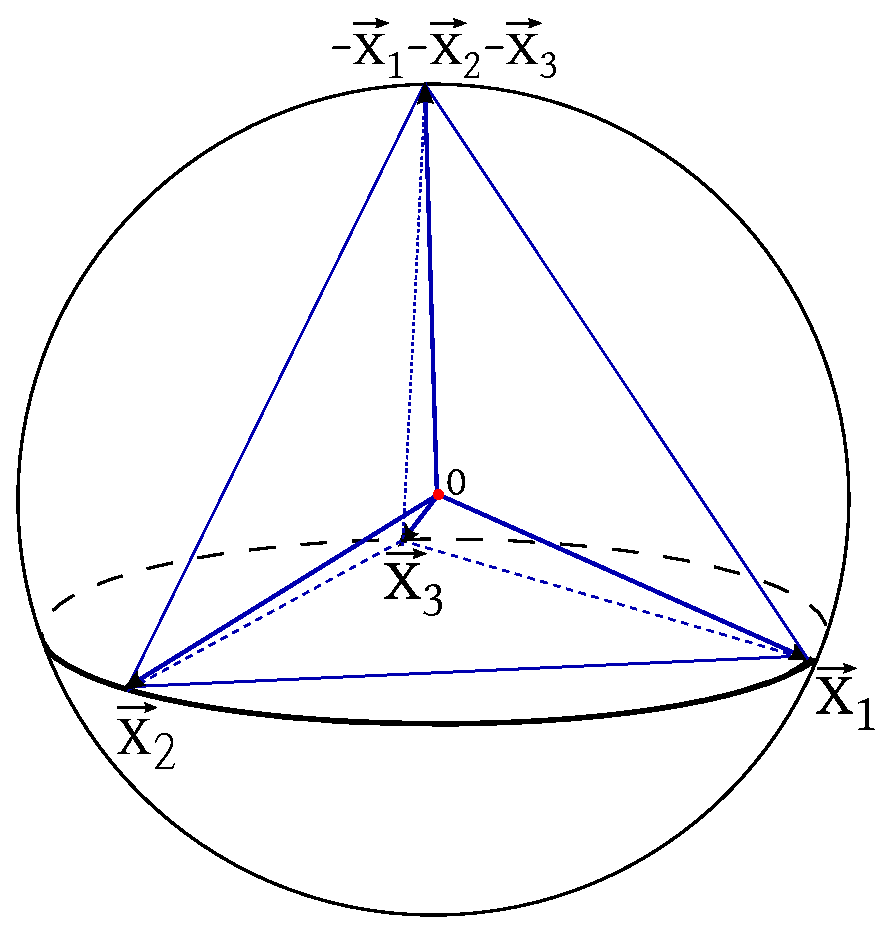
\includegraphics[scale=0.38]{tetrahedron}
	\caption[Balanced Configuration]{A regular tetrahedron ($3-$simplex) represents a balanced configuration for $k=3$.}
	\label{fig:Tetrahedron}
\end{figure}

\begin{corollary} \label{cor:NumberOfSolutions}
	Let $k,t$ be fixed. Then the expected number of solutions to the Configuration problem with input lists of size $|L|$ is
	\begin{equation} \label{eq:ExpNumberOfSolutions}
	\E[\# \text{solutions}] = \softO \left( |L|^k \Bigl(\frac{t^2}{k} \Bigl( \frac{k^2-t^2}{k^2-k} \Bigr)^{k-1}  \Bigr)^{\tfrac{n}{2}} \right).
	\end{equation}
\end{corollary}
\begin{proof}
	The total number of $k$-tuples is $|L|^k$. From Thms.~\ref{thm:WishartDist} and \ref{thm:maxConfig}, the probability that a random $k$-tuple forms a configuration from $\ConfSpacet$ is $\softO( \det(\Cbalt)^{n/2})$. Thm.~\ref{thm:maxConfig} states the value for this determinant.
\end{proof}

As a consequence, we can easily compute the size of input lists for a desired output list's size. In algorithms for \SVP, $t=1$ and the output list is required to have the same size as input lists. The following corollary proves the conjecture stated in \cite{BLS16}.

\begin{corollary} \label{cor:BalancedListSizes}
Let $k$ be fixed and $t=1$. In the Configuration problem, for the input lists each of size $|L|$, the output list is expected to be of size $|L|$ if $|L|  = \softO \Bigl( \Bigl( \frac{k^{\tfrac{k}{k-1}}}{k+1} \Bigr)^{\tfrac{n}{2}} \Bigr)$. 
\end{corollary}
\begin{proof}
	The statement immediately follows from setting the expression in Eq.~(\ref{eq:ExpNumberOfSolutions}) equal to $|L|$ for $t=1$. 
\end{proof}

Finally, we argue that solving the Configuration Problem gives a $1-\smallo(1)$ fraction of solutions for the $k$-List problem. This follows from Thm.~\ref{thm:maxConfig}. Essentially it states that for any fixed $\eps>0$, the probability that a randomly chosen solution to the approximate $k$-List problem forms a configuration $\eps$-close to $\Cbalt$, converges exponentially to $1$ as $n \rightarrow \infty$. Therefore, solving the $k$-List Configuration problem for $\CbalOne$ and restricting to only those solutions whose sum is at most $t$, gives a $1-\smallo(1)$ fraction of solutions for the approximate $k$-List problem. These arguments justify the following corollary.

\begin{corollary}\label{cor:ReductionToConfigProblem}
Let $k,t$ be fixed. Then the approximate $k$-List problem with target length $t$ can be solved in the same time as the $k$-List configuration problem with target configuration $\Cbalt$ for any fixed $\eps>0$.
\end{corollary}

\subsection{Algorithm} \label{subsec:KListAlgL2}

\begin{algorithm}[H]
\caption{$k$-List for the Configuration Problem}
\label{alg:AlgConfig}
\textbf{Input:} $L_1, \ldots, L_k$ -- lists of vectors from $\Sphere{n}$. $\Conf_{i,j}=\ScProd{\xvec_i}{\xvec_j} \in \R^{k \times k}$ -- Gram matrix. $\eps>0$. \\
\textbf{Output:} $\Lout$ -- list of $k$-tuples $\xvec_1 \in L_1, \ldots, \xvec_k \in L_k$, s.t.\ $\abs{\ScProd{\xvec_i}{\xvec_j}-\Conf_{ij}} \leq \eps$, for all $i,j$.

\begin{algorithmic}[1]

\State $\Lout \gets \{ \}$ 
\ForAll { $\xvec_1 \in L_1$}
	\ForAll {$j=2 \ldots k$}
		\State $L_j^{(1)} \gets$ \Call{Filter}{$\xvec_1, L_j, \Conf_{1,j}, \eps$} 
	\EndFor
	
	\ForAll {$\xvec_2 \in L_2^{(1)}$}
		\ForAll {$j=3 \ldots k$}
			\State $L_j^{(2)} \gets$ \Call{Filter}{$\xvec_2, L_j^{(1)}, \Conf_{2,j}, \eps$} 
		\EndFor	
		\State $\ddots$
		\Indent
			\ForAll {$\xvec_k \in L_k^{(k-1)}$}
				\State $\Lout \gets \Lout  \union \{(\xvec_1, \ldots \xvec_k)\}$
			\EndFor
		\EndIndent
	\EndFor
\EndFor 

\State{} \Return{$\Lout$} 
\end{algorithmic}
\vspace{10pt}
\begin{algorithmic}[1]
	\Function{Filter}{$\xvec, L, c, \eps$}
		\State $L' \gets \{ \}$
		\ForAll {$\xvec' \in L$}	
			\If{$\abs{\ScProd{\xvec}{\xvec'} - c}  \leq \eps$}
			 	\State $L' \gets L' \cup \{ \xvec' \}$
			\EndIf	
		\EndFor
		\State{} \Return $L'$
	\EndFunction
\end{algorithmic}

\end{algorithm}

Now we are ready to describe our algorithm for the Configuration problem given in Def.~\ref{def:ConfigProblem}.

On input the algorithm receives $k$ lists $L_1, \ldots, L_k$, a target configuration $\Conf$ in the form of a Gram matrix $\Conf_{i,j}=\langle{\xvec_i,}{\xvec_j}\rangle \in \R^{k \times k}$ and a small $\eps>0$.
The algorithm proceeds as follows: it picks an $\xvec_1 \in L_1$ and filters all the remaining lists with respect to the values $\ScProd{\xvec_1}{\xvec_i}$ for all $2 \leq i \leq k$.
More precisely, $\xvec_i \in L_i$ `survives' the filter if $\abs{\ScProd{\xvec_1}{\xvec_i} - \Conf_{1,i}}  \leq \eps$.
We put such an $\xvec_i$ into $L_i^{(1)}$ (the superscript indicates how many filters were applied to the original list $L_i$).
On this step, all the $k$-tuples of the form $(\xvec_1, \xvec_2, \ldots, \xvec_k) \in \{\xvec_1\} \times L_2^{(1)} \times \ldots \times L_k^{(1)}$ with the first vector $\xvec_1$ fixed partially match the target configuration. 
Most importantly, the lists $L_i^{(1)}$ become much shorter than the original ones. 

Next, we take $\xvec_2 \in L_2^{(1)}$ and create smaller lists $L_i^{(2)}$ from $L_i^{(1)}$ by filtering out all the $\xvec_i \in L_i^{(1)}$ that do not satisfy $\abs{\ScProd{\xvec_2}{\xvec_i} - \Conf_{2,i}}  \leq \eps$ for all $3 \leq i \leq k$.
A tuple of the form $(\xvec_1, \xvec_2, \xvec_3, \ldots, \xvec_k) \in \{\xvec_1\} \times \{\xvec_2\} \times L_3^{(2)} \times \ldots \times  L_k^{(2)}$ satisfies the target configuration $\Conf_{i,j}$ for $i=1,2$. Now we have the first two vectors fixed. 

We proceed with this list-filtering strategy until we have all $\xvec_i$ for $1\le i \le k$ fixed.
We output all the survived $k$-tuples.
Note that our algorithm becomes the trivial brute-force search algorithm once we are down to 2 lists $L_{k-1}^{(k-2)}, L_k^{(k-2)}$.
As soon as we have fixed $\xvec_1,\ldots,\xvec_{k-2}$ and created $L_{k-1}^{(k-2)},L_{k}^{(k-2)}$, we iterate over $L_{k-1}^{(k-2)}$ and check scalar products with every element from $L_{k}^{(k-2)}$. Our algorithm is detailed in Alg.~\ref{alg:AlgConfig}.

In Fig.~\ref{fig:AlgDescription}, we stress the difference between our algorithm (left) and the algorithm for the Configuration problem presented in \cite{BLS16} (right). While not being stated in terms of configurations, the BLS algorithm actually does search for tuples that form the balanced configuration but differently: for a fixed $\xvec_1$, it only filters the next list $L_2$ and the remaining $L_3, \ldots, L_k$ are left unchanged. Once $\xvec_2 \in L_2^{(1)}$ is chosen next, $L_3^{(2)}$ is obtained by applying filtering to the input $L_3$, while our Alg.~\ref{alg:AlgConfig} filters a smaller $L_3^{(1)}$. Certainly, in our approach we can miss some solutions that would be found by the BLS algorithm, but the results of Sect.~\ref{subsec:ConfigL2} show that this is a tiny fraction of solutions which vanishes in the asymptotics. To see the effect of this fact in practice, we refer the reader to Sect.~\ref{subsec:KListResults}.
\clearpage

\begin{figure}
\centering
\begin{subfigure}[t]{0.45\textwidth}
	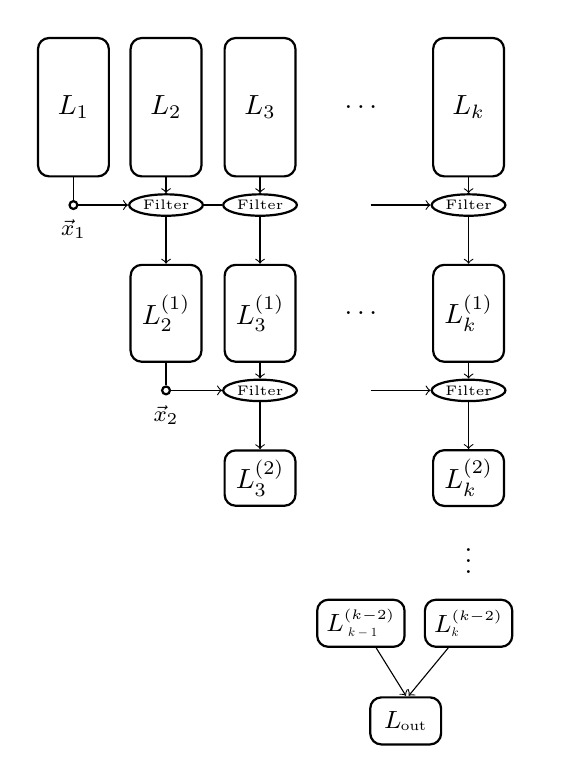
\begin{tikzpicture}
	\tikzset{
    List/.style={
    rectangle, 
    rounded corners, 
    draw=black, thick,
    minimum width=0.9cm, 
    text centered},
    Vertex/.style={
  	ellipse,
  	draw=black, thick,
  	inner sep=1pt},
	}
	\matrix (m) [row sep=2mm, column sep=2.3mm, name=m] {
		\node[List, minimum height=50pt] (L1) {$L_1$}; &
	 	\node[List, minimum height=50pt] (L2) {$L_2$}; &
		\node[List, minimum height=50pt] (L3) {$L_3$}; &	 	
	 	\node[] {$\ldots$}; &
	 	\node[List, minimum height=50pt] (Lk) {$L_k$}; \\
	 	
	 	\node[Vertex, label=below:{\footnotesize $\xvec_1$}] (x1) {}; &
	 	\node[Vertex] (l12) {\tiny Filter}; &
	 	\node[Vertex] (l13) {\tiny Filter}; &
	 	\node[] (dots1) {}; &
	 	\node[Vertex] (l1k) {\tiny Filter}; \\
	 	
	 	\node[] {}; &
	 	\node[List, minimum height=35pt] (L2p) {$L_2^{(1)}$}; &
		\node[List, minimum height=35pt] (L3p) {$L_3^{(1)}$}; &	 	
	 	\node[] {$\ldots$}; &
	 	\node[List, minimum height=35pt] (Lkp) {$L_k^{(1)}$}; \\
	 	
	 	\node[] {}; &
	 	\node[Vertex, label=below:{\footnotesize $\xvec_2$}] (x2) {}; &
	 	\node[Vertex] (l23) {\tiny Filter}; &
	 	\node[] (dots2) {}; &
	 	\node[Vertex] (l2k) {\tiny Filter}; \\
	 	
	 	\node[] {}; &
	 	\node[] {}; &
	 	\node[List, minimum height=20pt] (L3pp) {$L_3^{(2)}$}; &
	 	\node[] {}; &
	 	\node[List, minimum height=20pt] (Lkpp) {$L_k^{(2)}$}; \\
	 	
	 	\node[] {}; &
	 	\node[] {}; &
	 	\node[] {}; &
	 	\node[] {}; &
	 	\node[] {$\vdots$};\\
	 	
	 	\node[] {}; &
	 	\node[] {}; &
	 	\node[] {}; &
	 	\node[List, minimum height=17pt] (Llast1) {\small $L_{\scalebox{0.5}{ $k-1$}}^{\scriptscriptstyle(k-2)}$}; &
	 	\node[List, minimum height=17pt] (Llast2) {\small $L_{\scalebox{0.5}{$k$}}^{\scriptscriptstyle(k-2)}$};\\
	 	
	 	\node[minimum height=10pt] {}; &
	 	\node[] {}; &
	 	\node[] {}; &
	 	\node[] {}; &
	 	\node[] {}; & \\
	 	
	 	\node[minimum height=10pt] {}; &
	 	\node[] {}; &
	 	\node[] {}; &
	 	\multicolumn{2}{r}{\node[List, minimum height=17pt] (Lout) {\small $\Lout$};} \\
	 };
	%\node[fit=(m-9-3)(m-9-5)] (Lout) {\small $\Lout$};
	 \draw (L1) -- (x1);
	 \draw[->] (x1) -- (l12);
	 \draw[->] (L2) -- (l12);
	 \draw[->] (l12) -- (L2p);
	 
	 \draw (l12) -- (l13);
	 \draw[->](L3) -- (l13);
	 \draw[->] (l13) -- (L3p);
	 
	 \draw[->] (dots1) -- (l1k);
	 \draw[->] (Lk) -- (l1k);
	 \draw[->] (l1k) -- (Lkp);
	 
	 \draw (L2p) -- (x2);
	 \draw[->] (x2) -- (l23);
	 \draw[->] (L3p) -- (l23);
	 \draw[->] (l23) -- (L3pp);
	 
	 \draw[->] (dots2) -- (l2k);
	 \draw[->] (Lkp) -- (l2k);
	 \draw[->] (l2k) -- (Lkpp);
	 
	 \draw[->] (Llast1) -- (44pt, -112pt);
	 \draw[->] (Llast2) -- (45pt, -112pt);	
	 
\end{tikzpicture}
\caption{\footnotesize Pictorial representation of Alg.~\ref{alg:AlgConfig}. At level $i$, a filter receives as input $\xvec_i \in L_i^{(i-1)}$ and a vector $\xvec_{j}$ from $L_{j}^{(i-1)}$ (for the input lists, $L = L^{(0)}$). $\xvec_j$ passes through the filter if $\abs{\ScProd{\xvec_i}{\xvec_j} - \Conf_{i,j}}  \leq \eps$, in which case it is added to $L_{j}^{(i)}$. All the vectors from $L_j^{(i-1)}$ for all $j \leq i+1$ are processed in this manner. The configuration $\Conf$ and $\eps>0$ are global parameters.}
\label{fig:AlgDescription}
\end{subfigure} %
\quad \quad
\begin{subfigure}[t]{0.47\textwidth}
	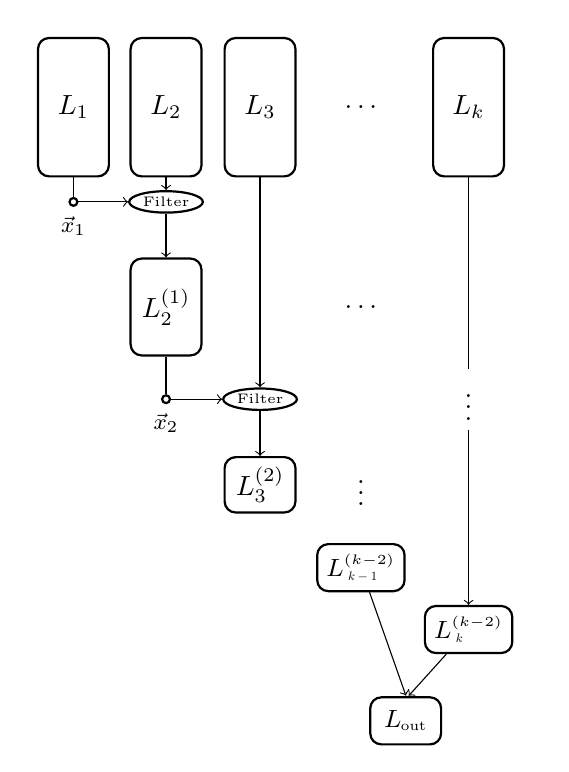
\begin{tikzpicture}
	\tikzset{
    List/.style={
    rectangle, 
    rounded corners, 
    draw=black, thick,
    minimum width=0.9cm, 
    text centered},
    Vertex/.style={
  	ellipse,
  	draw=black, thick,
  	inner sep=1pt},
	}
	\matrix (m) [row sep=1.6mm, column sep=2.3mm] {
		\node[List, minimum height=50pt] (L1) {$L_1$}; &
	 	\node[List, minimum height=50pt] (L2) {$L_2$}; &
		\node[List, minimum height=50pt] (L3) {$L_3$}; &	 	
	 	\node[] {$\ldots$}; &
	 	\node[List, minimum height=50pt] (Lk) {$L_k$}; \\
	 	
	 	\node[Vertex, label=below:{\footnotesize $\xvec_1$}] (x1) {}; &
	 	\node[Vertex] (l12) {\tiny Filter}; &
	 	\node[] (l13) {}; &
	 	\node[] (dots1) {}; &
	 	\node[] (l1k) {}; \\
	 	
	 	\node[] {}; &
	 	\node[List, minimum height=35pt] (L2p) {$L_2^{(1)}$}; &
		\node[] (L3p) {}; &	 	
	 	\node[] {$\ldots$}; &
	 	\node[] (Lkp) {}; \\
	 	
	 	\node[] {}; &
	 	\node[Vertex, label=below:{\footnotesize $\xvec_2$}] (x2) {}; &
	 	\node[Vertex] (l23) {\tiny Filter}; &
	 	\node[] (dots2) {}; &
	 	\node[] (l2k) {$\vdots$}; \\
	 	
	 	\node[] {}; &
	 	\node[] {}; &
	 	\node[List, minimum height=20pt] (L3pp) {$L_3^{(2)}$}; &
	 	\node[] {$\vdots$}; &
	 	\node[] (Lkpp) {}; \\
	 	
	 	\node[] {}; &
	 	\node[] {}; &
	 	\node[] {}; &
	 	\node[] {}; &
	 	\node[] {}; & \\[-1.3ex]
	 	
	 	\node[] {}; &
	 	\node[] {}; &
	 	\node[] {}; &
	 	\node[List, minimum height=17pt] (Llast1) {\small $L_{\scalebox{0.5}{ $k-1$}}^{\scriptscriptstyle(k-2)}$}; &
	 	\node[] {};\\
	 	
	 	\node[] {}; &
	 	\node[] {}; &
	 	\node[] {}; &
	 	\node[] {}; &
	 	\node[List, minimum height=17pt] (Llast2) {\small $L_{\scalebox{0.5}{ $k$}}^{\scriptscriptstyle(k-2)}$}; \\
	 	
	 	\node[minimum height=10pt] {}; &
	 	\node[] {}; &
	 	\node[] {}; &
	 	\node[] {}; &
	 	\node[] {}; & \\
	 	
	 	\node[minimum height=10pt] {}; &
	 	\node[] {}; &
	 	\node[] {}; &
	 	\multicolumn{2}{r}{\node[List, minimum height=17pt] (Lout) {\small $\Lout$};} \\
	 };
	 \draw (L1) -- (x1);
	 \draw[->] (x1) -- (l12);
	 \draw[->] (L2) -- (l12);
	 \draw[->] (l12) -- (L2p);
	 
	 %\draw (l12) -- (l13);
	 \draw[->](L3) -- (l23);
	 \draw[->] (l23) -- (L3pp);
	 
	 %\draw[->] (dots1) -- (l1k);
	 %\draw[->] (Lk) -- (l1k);
	 %\draw[->] (l1k) -- (Lkp);
	 
	 \draw (L2p) -- (x2);
	 \draw[->] (x2) -- (l23);
	 %\draw[->] (L3p) -- (l23);
	 %\draw[->] (l23) -- (L3pp);
	 
	 %\draw[->] (dots2) -- (l2k);
	 \draw[-] (Lk) -- (l2k);
	 \draw[->] (l2k) -- (Llast2);
	 \draw[->] (Llast1) -- (44pt, -112pt);
	 \draw[->] (Llast2) -- (45pt, -112pt);	
\end{tikzpicture}
\caption{\footnotesize The $k$-List algorithm given in \cite{BLS16}. The main difference is that a filter receives as inputs $\xvec_i$ and a vector $\xvec_j \in L_j$, as opposed to $\xvec_j \in L_j^{(i-1)}$. Technically, in \cite{BLS16}, $\xvec_i$ survives the filter if $\normalabs{\ScProd{\xvec_i}{\xvec_1+\ldots+\xvec_{i-1}}} \geq c_i$ for some predefined $c_i$. Due to our concentration results, this description is equivalent to the one given in \cite{BLS16} in the sense that the returned solutions are (up to a sub-exponential fraction) the same.}
\label{fig:AlgBLS}
\end{subfigure}
\caption[$k$-List algorithms for the Configuration problem]{$k$-List Algorithms for the Configuration Problem (Def.~\ref{def:ConfigProblem}). Left: Our Alg.~\ref{alg:AlgConfig}. Right: The algorithm from \cite{BLS16}}
\end{figure}

\clearpage

\subsection{Analysis} \label{subsec:KListAnalysisL2}

In this section we analyze the complexity of Alg.~\ref{alg:AlgConfig} for the Configuration problem. First, we should mention that the memory complexity is completely determined by the input list-sizes $\abs{L_i}$ (remember that we restrict to constant $k$) and the application of $k$ filters does not change the asymtotics. In practice, all intermediate lists $L_i^{(j)}$ can be implemented by storing pointers to the elements of the original lists. 

In the following, we compute the expected sizes of filtered lists $L_i^{(j)}$ and establish the expected running time of Alg.~\ref{alg:AlgConfig}. Since our algorithm has an exponential running time $2^{cn}$ for some $c = \Theta(1)$, we are interested in determining $c$. We ignore polynomial factors, e.g.\ we do not take into account time spent for computing inner products. 

\begin{thm}\label{thm:RunTimeAlg1}
Let $k$ be fixed. Alg.~\ref{alg:AlgConfig} given as input $k$ lists $L_1, \ldots, L_k \subset \Sphere{n}$ of the same size $\abs{L}$, a target balanced configuration $\Cbalt \in \R^{k \times k}$, a target length $0 < t < \sqrt{k}$, and $\eps > 0$, outputs the list $\Lout$ of solutions to the Configuration problem. The expected running time of Alg.~\ref{alg:AlgConfig} is
	\begin{equation}\label{eq:RunTime}
	 T =  \softO \Bigl( \abs{L} \cdot \max\limits_{1 \leq i \leq k-1}  \abs{L}^i \cdot \frac{(k^2-t^2)^i}{(k^2-k)^{i+1}}  \cdot \Bigl( \frac{(k^2 - k + (i-1)(t^2-k))^2}{k^2 - k +(i-2)(t^2-k)} \Bigr)^{\frac{n}{2}} \Bigr).
  \end{equation}
In particular, for $t=1$ and $\abs{\Lout} = \abs{L}$ it holds that
  \begin{equation}\label{eq:RunTime=1}
	 T = \softO \biggl( \Bigl( \frac{k^{ \frac{1}{k-1} }}{k+1} \cdot  \max\limits_{1 \leq i \leq k-1} k^{\frac{i}{k-1}} \cdot \frac{(k-i+1)^2}{k-i+2}  \Bigr)^{\frac{n}{2}} \biggr).
  \end{equation}
\end{thm}

\begin{remark}\label{rmk:RunningTimeOfBLS} In the proof below we also show that the expected running time of 
the BLS
$k$-List algorithm 
from \cite{BLS16} for $t=1,\abs{\Lout}=\abs{L}$ is
\begin{equation} \label{eq:RunTimeBLS}
	T_{\text{BLS}} = \softO \Bigl(  \Bigl( \frac{k^{\frac{k}{k-1}}}{(k+1)^2} \cdot \max\limits_{1 \leq i \leq k-1} \bigl( k^{\frac{i}{k-1}} \cdot (k-i+1) \bigr)\Bigr)^{\frac{n}{2}} \Bigr).
\end{equation}
\end{remark} 

\begin{proof}[Proof of Thm.~\ref{thm:RunTimeAlg1}]
	The correctness of the algorithm is straightforward: let us associate the lists $L^{(i)}$ with a level $i$, where $i$ indicates the number of filtering steps applied to $L$ (we identify the input lists with the $0\th$ level: $L_i=L^{(0)}_i$). So for executing the filtering for the $i\th$ time, we choose an $\xvec_{i} \in L_{i}^{(i-1)}$ that satisfies the condition $\abs{\ScProd{\xvec_i}{\xvec_{i-1}} - C_{i,i-1}} \leq \eps$ (for a fixed $\xvec_{i-1}$) and append to a previously obtained $(i-1)$-tuple $(\xvec_1, \ldots, \xvec_{i-1})$. Thus, on the last level, we put into $\Lout$ a $k$-tuple $(\xvec_1, \ldots, \xvec_{k})$ that is a solution to the Configuration problem. To make the subscripts less confusing, we set $C = \Cbalt$ throughout the proof. 
	
	Let us first estimate the size of the list $L_i^{(i-1)}$ output by the filtering process applied to the list $L_i^{(i-2)}$ for $i>1$ (i.e.\ the left-most lists in Fig.~\ref{fig:AlgDescription}). Recall that all $\xvec_i \in L_i^{(i-1)}$ satisfy $\abs{\ScProd{\xvec_i}{\xvec_{j}} - C_{i,j}} \leq \eps$, $1 \leq j \leq i-1 $. Then the \emph{total} number of $i$-tuples $(\xvec_1, \xvec_2, \ldots, \xvec_i) \in L_1 \times L_2^{(1)} \times \ldots \times L_i^{(i-1)}$ considered by the algorithm is determined by the probability that in a random $i$-tuple, all pairs $(\xvec_j, \xvec_{j'}), 1 \leq j,j' \leq i$ satisfy the inner product constraints given by $C_{j,{j'}}$. This probability is given in Thm.~\ref{thm:WishartDist} and, since the input lists are of the same size $\abs{L}$, we have\footnote{Throughout this proof, the equations that involve list-sizes $\abs{L}$ and running time $T$ are assumed to have $\softO(\cdot)$ on the right-hand side. We omit it for clarity.}
	\begin{align}\label{eq:ProductOfListSizes}
			\normalabs{L_1} \cdot \normalabs{L_2^{(1)}} \cdot \ldots \normalabs{L_i^{(i-1)}} = \normalabs{L}^i \cdot  \det (C[1 \ldots i])^{\frac{n}{2}},
	\end{align}	
where $\det(C[1 \ldots i])$ denotes the $i$-th principal minor of $C$.
Using Eq.~\eqref{eq:ProductOfListSizes} for two consecutive values of $i$ and dividing one equation by the other, we obtain
	\begin{align}\label{eq:IntermSize}
		\normalabs{L_{i+1}^{(i)}} = \abs{L} \cdot \Bigl( \frac{\det (C[1 \ldots i+1]}{\det (C[1 \ldots i])} \Bigr)^{\frac{n}{2}}.
	\end{align}
Note that these expected list sizes can be smaller than 1. This should be thought of as the inverse probability that the list is not empty.
Since our target is a balanced configuration $\Cbalt$, the entries of the input Gram matrix are specified by Thm.~\ref{thm:maxConfig} and, hence, we compute the determinants in the above quotient by applying Lemma~\ref{lem:CBalancedDet} with $a = \frac{t^k-k}{k^2-k}$. Again, from the shape of the Gram matrix $\Cbalt$ and the equally-sized input lists, it follows that the filtered list on each level are of the same size: $\normalabs{L_{i+1}^{(i)}} = \normalabs{L_{i+2}^{(i)}} = \ldots = \normalabs{L_k^{(i)}}$. Therefore, for all filtering levels $0 \leq j \leq k-1$ and for all $j+1 \leq i \leq k$,
  \begin{equation}\label{eq:IntermSizeExpanded}
	 \bigabs{L_i^{(j)}} = \abs{L} \cdot \Bigl( \frac{k^2 - t^2}{k^2 - k} \cdot \frac{k^2 - k + j(t^2-k)}{k^2 - k +(j-1)(t^2-k)} \Bigr)^{ \frac{n}{2} }.
  \end{equation}
Now let us discuss the complexity of the algorithm. Clearly, the running time of Alg.~\ref{alg:AlgConfig} is (up to sub-exponential factors in $n$) 
\begin{align*}
   T = \normalabs{L_1^{(0)}} \cdot (\normalabs{L_2^{(0)}} + \normalabs{L_2^{(1)}} \cdot (\normalabs{L_3^{(1)}} +\normalabs{L_3^{(2)}} \cdot(\ldots \cdot (\normalabs{L_k^{(k-2)}} + \normalabs{L_k^{(k-1)}} ) )).
\end{align*}  
Multiplying out and observing that $\normalabs{L_k^{(k-2)}}>\normalabs{L_k^{(k-1)}}$ (so creating a filtered list takes longer than enumerating over it), we may ignore the very last term and deduce that the total running time is (up to sub-exponential factors) given by

  \begin{equation} \label{eq:RunTimeProof}
  	T =  \abs{L} \cdot \max\limits_{1 \leq i \leq k-1}  \normalabs{L^{(i-1)}} \cdot \prod_{j=1}^{i-1} \normalabs{L^{(j)}},
  \end{equation}
  where $\normalabs{L^{(j)}}$ is the size of any filtered list on level $j$ (so we omit the subscripts). Consider the value $\im$ of $i$, where the maximum is attained in the above formula. The meaning of $\im$ is that the total cost over all loops to create the lists $L_j^{(\im)}$ dominates the running time. At this level, the lists $L_j^{(\im)}$ become small enough such that iterating over them (i.e.\ creating $L_j^{(\im+1)}$) does not contribute to the asymptotics. Plugging in Eqns.~\eqref{eq:ProductOfListSizes} and \eqref{eq:IntermSize} into Eq.~\eqref{eq:RunTimeProof}, we obtain
  \vspace{-1ex}
  \begin{equation}\label{eq:TotalRunningTimeViaDets}
    T=\abs{L}\cdot \max\limits_{1\le i \leq k-1} \normalabs{L}^i \Bigl( \frac{(\det C[1\ldots i])^2}{\det C[1\ldots (i-1)]}\Bigr)^{\frac{n}{2}}.
  \end{equation}
  From Lemma~\ref{lem:CBalancedDet}, $\det C[1\ldots i] = \Bigl( 1 + (i-1)\frac{t^2-k}{k^2-k})\Bigr) \Bigl( \frac{k^2-t^2}{k^2-k} \Bigr)^{i-1}$, giving us the desired expression for the running time.
  
  For the case $t=1$ and $\normalabs{\Lout} = \normalabs{L}$, the result of Cor.~\ref{cor:BalancedListSizes} on the size of the input lists $\abs{L}$ yields a compact formula for the filtered lists:
    \vspace{-1ex}
    \begin{equation}\label{eq:IntermSize_t=1}
    	\bigabs{L_i^{(j)}} =  \Bigl( k^{\frac{1}{k-1}} \cdot \frac{k-j}{k-j+1} \Bigr)^{\tfrac{n}{2}}.
    \end{equation}
    Plugging this into either Eq.~\eqref{eq:RunTimeProof} or Eq.~\eqref{eq:TotalRunningTimeViaDets}, the running time stated in Eq.~\eqref{eq:RunTime=1} easily follows.
    
    It remains to show the complexity of the BLS algorithm \cite{BLS16}, claimed in Rmk.~\ref{rmk:RunningTimeOfBLS}. The algorithm is illustrated in Fig.~\ref{fig:AlgBLS}. We change the presentation of the algorithm to our configuration setting: in the original description, a vector $\xvec_i$ survives the filter if it satisfies $\abs{ \ScProd{\xvec_i}{\xvec_1 + \ldots + \xvec_{i-1}}} \geq c_i$ for a predefined $c_i$ (a sequence $(c_1, \ldots, c_{k-1}) \in \R^{k-1}$ is given as input to the BLS algorithm). Our concentration result (Thm.~\ref{thm:WishartDist}) also applies here and the condition $\abs{ \ScProd{\xvec_i}{\xvec_1 + \ldots + \xvec_{i-1}}} \geq c_i$ is equivalent to a pairwise constraint on the scalar product $\ScProd{\xvec_i}{\xvec_j}$ up to losing an exponentially small fraction of solutions. The optimal sequence of $c_i$'s corresponds to the configuration $\Cbalt$ derived in Thm.~\ref{thm:maxConfig}.
    
    Indeed, Table 1 in \cite{BLS16} matches $\Cbalt$ (case $t=1$) exactly. So we may rephrase their filtering where instead of shrinking the list $L_i$ by taking inner products with the sum $\xvec_1+ \ldots + \xvec_{i-1}$, we filter $L_i$ by considering $\ScProd{\xvec_i}{\xvec_j}$ for $1 \leq j \leq i-1$. 
      
    It follows that the filtered lists $L^{(i)}$ on level $i$ are of the same size (in leading order) for both our and BLS algorithms.
    In particular, Eq.~\eqref{eq:IntermSize} holds for the expected list-sizes of the BLS algorithm.
    
    The crucial difference lies in the construction of these lists. To construct the list $L_i^{(i-1)}$ in BLS, the filtering procedure is applied not to $L_i^{(i-2)}$ but to a (larger) input-list $L_i$. Hence, the running time of the BLS algorithm ignoring sub-exponential factors, is (cf.\ Eq.~\eqref{eq:RunTimeProof})
      \begin{align*}
      	 T_{BLS} = 
      	 \normalabs{L_1} \cdot (\normalabs{L_2} + \normalabs{L_2^{(1)}} \cdot ( \normalabs{L_3} +\normalabs{L_3^{(2)}}  \cdot(\ldots \cdot (\normalabs{L_k} + \normalabs{L_k^{(k-1)}} ) ))
    	 =
      	 \normalabs{L}^2 \cdot \max\limits_{1 \leq i \leq k-1} \cdot \prod_{j=1}^{i-1} \normalabs{L^{(j)}}.
      \end{align*}
    The result follows after substituting Eq.~\eqref{eq:IntermSize_t=1} into the above product. 
\end{proof}

Both runtime expressions, Eq.~\eqref{eq:RunTime} for Alg.~\ref{alg:AlgConfig} and Eq.~\eqref{eq:RunTimeBLS} for the BLS algorithm, can be easily evaluated given $k$ and $\normalabs{L}$, see Fig.~\ref{fig:RunTimes}. The input list-sizes $\normalabs{L}$ are chosen to guarantee $\normalabs{\Lout} = \normalabs{L}$ on expectation.

\begin{SCfigure}[1.2]
	\centering
	\includegraphics[scale=0.2]{kListRunTimesCompare}
	\hspace{4ex}
	\caption[Runtime exponents for $k$-List algorithms]{Running time exponents scaled by $1/n$ for the target length $t=1$. For $k=2$, both algorithms are the Nguyen-Vidick sieve \cite{NguVid08} with $\log(T)/n = 0.415$ (naive brute-force over two lists). For $k=3$, Algorithm \ref{alg:AlgConfig} achieves $\log(T)/n = 0.3962$, the BLS algorithm has $\log(T)/n = 0.4812$. \vspace{10ex}} \label{fig:RunTimes}
\end{SCfigure}

Our algorithm can be further improved by applying Locality-Sensitive Hashing techniques similar to \cite{SODA:BDGL16} to shorten the lists prior to filtering. Unfortunately, the gain is very modest: for $k=3, t=1$, we can get the running time down from $2^{0.3962n + \smallo(n)}$ to $2^{0.3717n + \smallo(n)}$. The details on this extension are presented in \cite{HK}.

We remark that it seems quite challenging to analyze the $k$-List algorithms for a \emph{non-fixed} $k$. Our approach heavily relies on the fact that $k$ is a fixed constant allowing to suppress all the pre-factors in both run-times and list sizes in the $\softO_k(\cdot)$ notation. Indeed, taking a closer look at the suppressed pre-factors, we immediately notice that they depend at least \emph{exponentially} on $k$ (see, for example, the expression for $W_{n,k}$ in Thm.~\ref{thm:WishartDist}). Being able to let $k \rightarrow \infty$ would, however, greatly contribute to our understanding of complexity of \SVP as it would enable us to compare sieving techniques with enumeration. 

Further, we do not know what is an optimal choice of $\eps$ given $k$ and $\normalabs{L}$. In Sect.~\ref{subsec:KListResults}, we present our experimental results for Alg.~\ref{alg:AlgConfig}, where we just try several $\eps$'s.

\subsection{Approximate Shortest Vector Problem} \label{subsec:ApproxSVP}

In this section we expound the connection between the approximate $k$-List problem in Euclidean norm (Def.~\ref{def:kListL2}) and the approximate Shortest Vector Problem, $\appSVP$, for a constant approximation factor $\gamma$. Recall the definition of the latter problem.

On input, we are given a full-rank lattice $\mathcal{L}(B)$ described by a matrix $B \in \R^{n \times n}$ (with polynomially-sized entries) and some constant $\gamma > 1$. The task is to output a non-zero lattice vector $\xvec \in \mathcal{L}(B)$ s.t.\ $ \| \xvec \| \leq \gamma \lambda_1 (B)$. $\xvec$ is a solution to the approximate shortest vector problem. Since the solution is not unique, we are fine with any vector that satisfies the length condition.

The family of so-called sieving (or \AKS) algorithms, described in the pioneering work of Ajtai, Kumar, and Sivakumar \cite{STOC:AjtKumSiv01}, offers the best known to-date heuristic algorithm for $\appSVP$. The fact that this algorithm achieves a single-exponential running time and memory complexity was already stated in the original paper \cite{STOC:AjtKumSiv01}, but a more precise analysis of the constant in the exponent has a long history. The result of Nguyen and Vidick in \cite{NguVid08}, stating the running time of order $2^{5.9n + \smallo(n)}$,  was later improved by Pujol and Stehl\'e to $2^{2.465n + \smallo(n)}$ running time and $2^{1.42n + \smallo(n)}$ space \cite{PujSte09}. Under an assumption on the distribution of lattice-vectors under sieving, we are able to \emph{heuristically} solve $\appSVP$ in $2^{0.415n + \smallo(n)}$ time and $2^{0.208n + \smallo(n)}$ space. Finally, the currently best known running time of  $2^{0.292n + \smallo(n)}$ in \cite{SODA:BDGL16} comes from a line of works based on the techniques from Locality-Sensitive Hashing. This is to be compared with the fastest \emph{provable} $\appSVP$ solver by Aggarwal et al.\ \cite{STOC:ADRS15}. Based on the so-called discrete Gaussian sampling, this algorithm achieves $2^{n + \smallo(n)}$-time and space complexity. 

Practically, however, sieving algorithms are less attractive than Kannan's enumeration with running time of order $2^{\bigO(n \log n)}$. This fact is attributed to exponential memory requirement of sieving (and also to the advances in pruning techniques for enumeration). Recently, Bai, Laarhoven, Stehl\'e aiming at reducing memory, presented a variant of sieving algorithm with space complexity of $2^{0.1887n+\smallo(n)}$ -- an exponential improvement over the previous $2^{0.208n + \smallo(n)}$-space sieving algorithm. Yet the gain comes at cost of increased running time: $2^{0.4812n + \smallo(n)}$ as opposed to $2^{0.415n +\smallo(n)}$ (for non-LSH sieving). To understand the BLS algorithm and how our improved $k$-List solver gives a faster sieving algorithm, we briefly explain how the \AKS algorithm works. 

\paragraph{The Nguyen-Vidick sieve.} Sieving algorithms have two flavours: the Nguyen-Vidick sieve \cite{NguVid08} and the Gauss sieve \cite{STOC:MicVou10}. Both make $\poly(n)$ number of calls to the approximate $2$-List solver. The Nguyen-Vidick sieve starts by sampling lattice-vectors $\xvec \in \Lat(B) \cap \Ball(\zerovec, 2^{\bigO(n)} \cdot \lambda_1(B))$. This can be done using, for example, Klein's sampling procedure \cite{SODA:Klein00} that outputs a lattice-vector of length not greater than $2^{\bigO(n)} \cdot \lambda_1(B)$.  In the $2$-List Nguyen-Vidick sieve, we sample many such lattice-vectors, put them in a list $L$, and search for \emph{pairs} $\xvec_1 \times \xvec_2 \in L \times L$ s.t. $\| \xvec_1 \pm \xvec_2 \| \leq (1-\eps) \max\{\| \xvec_1 \|, \| \xvec_2 \|\}$ for some small $\eps>0$. The sum is put into $\Lout$. The size of $L$ is chosen in a way to guarantee $\normalabs{L} \approx \normalabs{\Lout}$. The search for pairs is repeated over the list $\Lout$ once it is large enough. 

The size of $L$ determines the space complexity of the algorithm. A natural way to shorten the size of the input list $L$ is, instead of looking for pairs, look for triples, or, more general, $k$-tuples that form a short sum. Indeed, it easily follows from Cor.~\ref{cor:BalancedListSizes} that the larger $k$ is, the fewer vectors we should sample for the starting list  $L$ in order to expect $\normalabs{\Lout} = \normalabs{L}$. 

So the Nguyen-Vidick can be generalized to the search for $k$-tuples $\xvec_1, \ldots, \xvec_k \in L \times \ldots \times L$ s.t.\ $\| \xvec_1 + \ldots + \xvec_k \| \leq (1-\eps) \max_{1 \leq i \leq k} \{\| \xvec_i\|\}$. Now the sum $\xvec_1 + \ldots + \xvec_k$ is put into $\Lout$ and the search for $k$-tuples is repeated over $\Lout$. Note that since with each new iteration we obtain vectors that are shorter by a constant factor $(1-\eps)$, starting with $2^{\bigO(n)}$ approximation to the shortest vector (a property guaranteed by Klein's sampler applied to an \LLL-reduced basis), we need only $\poly(n)$ iterations to find the desired $\xvec \in \Lat(B)$.

Naturally, we can apply our Alg.~\ref{alg:AlgConfig} to $k$ copies of the list $L$ to implement the search for short sums. We do so by making a commonly used assumption: we assume the sampled lattice-vectors we put into the list lie uniformly on a spherical shell (on a very thin shell, essentially a sphere). The heuristic here is that it does not affect the behaviour of the algorithm. Intuitively, the discreteness of a lattice should not be `visible' to the algorithm (at least not in the search for the approximate shortest vector; as soon as we see the discreteness, the vectors are already short enough). We refer to \cite{NguVid08} for a more exhaustive discussion on this heuristic. 

The advantage in using our Alg.~\ref{alg:AlgConfig} instead of the BLS $k$-List search within an \appSVP algorithm is straightforward: the search for a `good' $k$-tuple is the routine that determines the complexity of the algorithm. So any improved algorithm for the approximate $k$-List problem immediately leads to a better \appSVP algorithm. 

\paragraph{Gauss sieve.} More interestingly, our improved $k$-List algorithm for $k \geq 3$ can as well be used within the Gauss sieve, which is known to perform faster in practice than the Nguyen-Vidick sieve. Let us briefly recall the Gauss sieve algorithm.

An iteration of the original 2-Gauss sieve as described in \cite{STOC:MicVou10}, searches for pairs $(\pvec, \vvec)$ s.t.\ $\| \pvec + \vvec \| < \max \{\| \pvec \|, \| \vvec \| \}$, where $\pvec \in \mathcal{L}(B)$ is \emph{fixed}, $\vvec \in L \subset \mathcal{L}(B)$, and $\pvec \neq \vvec$. Once such a pair is found and $\| \pvec \| > \| \vvec \|$, we reduce $\pvec$ by setting $\pvec'  \leftarrow \pvec + \vvec$ and proceed with the search over $(\pvec', \vvec)$, otherwise if $\| \pvec \| < \| \vvec \|$, we delete $\vvec \in L$ and store the sum $ \pvec + \vvec$ as $\pvec$-input point for the next iteration. Once no pair is found, we add $\pvec'$ to $L$. On the next iteration, the search is repeated with another $\pvec$ which is obtained either by reducing some previously deleted $\vvec \in L$, or by sampling from $\mathcal{L}(B)$. The idea is to keep only those vectors in $L$ that \emph{cannot} form a pair with a shorter sum. Bai, Laarhoven, and Stehl\'{e}  in \cite{BLS16}, generalize it to the $k$-Gauss sieve by keeping only those vectors in $L$ that do not form a shorter $k$-sum. In the language of configuration search, we look for configurations $(\pvec, \vvec_1, \ldots, \vvec_{k-1}) \in \pvec \times L \times \ldots \times L$ where the first point is fixed, so we apply our Alg.~\ref{alg:AlgConfig} on $k-1$ (identical) lists.

Pseudo-code for $3$-Gauss sieve is given in Alg.~\ref{alg:3GaussSieve} below. We assume the approximation $\gamma \lambda_1(B)$ is given as input. The main procedure (first lines 1-11) is exactly the same as in the original algorithm of Micciancio-Voulgaris. The difference is in the main subroutine $\Call{TripleReduce}$ that implements the approximate $3$-List search with the first vector in a triple being $\pvec$. The list $L$ is always kept sorted so that at the end of the procedure the shortest vector in the list is $L[1]$.
The algorithm can be easily generalized to the larger $k$, but we decided to present $k=3$ case as the most practically relevant. The experimental results on $3$-Gauss sieve are given in the next section.

\begin{algorithm}[t]
\caption{$3$-Gauss sieve}
\label{alg:3GaussSieve}
\textbf{Input:} $B \in \R^{n \times n}$ - an \LLL-reduced lattice basis, $\gamma \lambda_1(B)$ - the desired approximation factor, $\eps>0$ \\
\textbf{Output:} $\xvec \in \Lat(B)$ s.t.\ $\| \xvec \| \leq \gamma \lambda_1 (B)$

\begin{algorithmic}[1]
	\State $L \gets \{\}$ \Comment Sorted list of triple-reduced vectors
	\State $S \gets \{\}$ \Comment Stack of vectors
	\While{($L[1] > \gamma \lambda_1(B)$)}
		\If{$S$ is not empty}
			\State $\pvec \gets S.\text{pop()}$
		\Else
			\State $\pvec \gets \text{KleinSample}(B)$ \Comment Sample a vector from $\Lat(B)$
		\EndIf
		\State $\pvec' \gets $ \Call{TripleReduce}{$\protect \pvec, L, s$}
		\If{$\pvec' \neq \zerovec$}
			\State $L \gets L \union \{ \pvec'\}$
		\EndIf
	\EndWhile
	\State \Return $L[1]$
\end{algorithmic}

\vspace{10pt}

\begin{algorithmic}[1]
	\Function{TripleReduce}{$\protect \pvec, L, S$}
		\While{($\pvec$ cannot be reduced)} \Comment Try to reduced $\pvec$ first
			\State $L' \gets $ \Call{Filter}{$ \protect \pvec, L, \eps$}
			\ForAll{$\vvec_1, \vvec_2 \in L' \times L'$}
				\If{$\| \pvec \pm \vvec_1 \pm \vvec_2 \| < \| \pvec \|$}
					\State $\pvec \gets \vvec_1 \pm \vvec_2$ \Comment the sign should satisfy the If-condition
				\EndIf
			\EndFor
		\EndWhile
		\State $L' \gets $ \Call{Filter}{$ \protect \pvec, L$} \Comment with a new reduced $\pvec$
		\ForAll{$\vvec_1, \vvec_2 \in L' \times L'$}
			\If{$\| \pvec \pm \vvec_1 \pm \vvec_2 \| < \max \{ \| \vvec_1 \|, \| \vvec_2 \| \} $}
				\State $\max \{ \| \vvec_1 \|, \| \vvec_2 \| \} \gets \pvec \pm \vvec_1 \pm \vvec_2$
			\EndIf
		\EndFor
		\State \Return $\pvec$
	\EndFunction
\end{algorithmic}

\vspace{10pt}

\begin{algorithmic}[1]
	\Function{Filter}{$\protect \pvec, L, \eps$} \Comment Filter w.r.t.\@ balanced configuration $\Cbalt$
		\State $L' \gets \{ \}$
		\ForAll{$\vvec \in L$}
			\If{$\big| \frac{\langle \vvec, \pvec \rangle}{\|\vvec \| \|\pvec \|} \big| \geq \frac{1}{3} - \eps$}
				\State $L' \gets L' \union \{ \vvec \}$
			\EndIf
		\EndFor
		\State \Return $L'$
	\EndFunction
\end{algorithmic}

\end{algorithm}

\clearpage

\subsection{Experimental results} \label{subsec:KListResults}
We implement the $3$-Gauss sieve Algorithm~\ref{alg:3GaussSieve} in collaboration with S.\ Bai \cite{Bai16}. 
The implementation is based on the program developed by Bai, Laarhoven, and Stehl\'{e} in \cite{BLS16}. 
The experiments are run on the Ruhr University C3 cluster \cite{C3}. The results are presented in Table~\ref{table:kListExperiments}.

Lattice bases are generated by the \SVP challenge generator \cite{SVPChallenge}. It produces a lattice generated by the columns of the matrix
\begin{align*} B=
\begin{psmallmatrix}
	p & x_1 & \ldots & x_{n-1} \\
	0 & 1 & \ldots &  0  \\
	\vdots & \vdots & \ddots & \vdots \\
	0 & 0 & \ldots & 1 \\
\end{psmallmatrix},
\end{align*}
where $p$ is a large prime, and $x_i< p$ for all $i$. Lattices of this type are random in the sense of Goldstein and Mayer \cite{GoldMay06}.

For all the dimensions except $n=80$, the bases are preprocessed with \BKZ reduction of block-size~$20$. For $n=80$, the block-size is $30$. For our input lattices, we do not know their minimum $\lambda_1$. The algorithm terminates when it finds many linearly dependent triples $(\pvec, \vvec_1, \vvec_2)$. It means that at some point $\Call{TripleReduce}$ starts outputting $\zerovec$. We set a counter for such an event and terminate the algorithm once this counter goes over a pre-defined threshold. The intuition behind this idea is straightforward: at some point the list $L$ will contain very short basis-vectors and the remaining list-vectors will be their linear combinations. Trying to reduced the latter will ultimately produce the zero-vector. The same termination condition was already used in \cite{BLM15}, where the authors experimentally determine a threshold of such `zero-sum' triples.

Up to $n=64$, the experiments are repeated 5 times (i.e.\ on 5 random lattices), for the dimensions less than $80$, 3 times. For the running times and the list-sizes presented in the table below, the average is taken. For $n=80$, the experiment was performed once.  

Our tests confirm a noticeable speed-up of the 3-Gauss sieve when our Configuration Search Algorithm~\ref{alg:AlgConfig} is used. Moreover, as the analysis suggests (see Fig.~\ref{fig:RunTimes}), our algorithm outperforms the naive 2-Gauss sieve while using much less memory. 

Another interesting aspect of the algorithm is the list-sizes when compared with BLS. Despite the fact that asymptotically the size of the list $|L|$ is the same for our and for the BLS algorithms, in practice our algorithm requires a longer list (cf.\ the right numbers in each column). This is due to the fact that we filter out a larger fraction of solutions. Also notice that increasing $\eps$ -- the approximation to the target configuration -- we achieve an additional speed-up. This becomes obvious once we look at the $\Call{Filter}$ procedure: allowing for a smaller inner-product throws away less vectors, which in turn results in a shorter list $L$. For the range of dimensions we consider, the optimum is attained at $\eps=0.3$.

\renewcommand{\arraystretch}{1.9}
\begin{table}[t]
	\centering
	\resizebox{\textwidth}{!}{%
	\begin{tabular}{|c|c|c|c|c|c|c|} \hline
		 & \multirow{2}{*}{$2$-sieve} & \multirow{2}{*}{BLS $3$-sieve} & \multicolumn{4}{c|}{ Alg.~\ref{alg:3GaussSieve}, $3$-sieve} \\ \cline{4-7}
		& & & $\eps = 0.0$ & $\eps = 0.015$ & $\eps = 0.3$ & $\eps = 0.4$ \\ \hline
		$n$ & $T$, $\normalabs{L}$ & $T$, $\normalabs{L}$ & $T$, $\normalabs{L}$ & $T$, $\normalabs{L}$ & $T$, $\normalabs{L}$ & $T$, $\normalabs{L}$ \\ \hline
		60 & 1.38e3, 13257 & 1.02e4, 4936& 1.32e3, 7763& 1.26e3, 7386& 1.26e3, 6751 & \textbf{1.08e3, 6296} \\ \hline
		62 & 2.88e3, 19193 & 1.62e4, 6239 & 2.8e3, 10356 & 3.1e3, 9386 & \textbf{1.8e3, 8583} & 2.2e3, 8436 \\ \hline
		64 & 8.64e3, 24178 & 5.5e4, 8369 & 5.7e3, 13573& 3.6e3, 12369 & \textbf{3.36e3, 11142}& 4.0e4, 10934\\ \hline
		66 & 1.75e4, 31707 & 9.66e4, 10853 & 1.5e4, 17810 & 1.38e4, 16039 & \textbf{9.1e3, 14822}& 1.2e4, 14428 \\ \hline
		68 & 3.95e4, 43160 & 2.3e5, 14270 & 2.34e4, 24135 & 2.0e4, 21327 & \textbf{1.68e4, 19640}& 1.86e4, 18355 \\ \hline
		70 & 6.4e4, 58083 & 6.2e5, 19484 & 6.21e4, 32168 & 3.48e5, 26954 & \textbf{3.3e4, 25307} & 3.42e4, 24420 \\ \hline
		72 & 2.67e5, 77984 & 1.2e6, 25034& 7.6e4, 40671 & 7.2e4, 37091 & \textbf{6.16e4, 34063} & 6.35e4, 34032 \\ \hline
		74 & 3.45e5, 106654 & \textemdash& 2.28e5, 54198& 2.08e5, 47951& \textbf{2.02e5, 43661}& 2.03e5, 40882\\ \hline
		76 & 4.67e5, 142397 & \textemdash& 3.58e5, 71431& 2.92e5, 64620& \textbf{2.42e5, 56587} & 2.53e5, 54848 \\ \hline
		78 & 9.3e5, 188905 & \textemdash & \textemdash & \textemdash& \textbf{4.6e5, 74610} & 4.8e5, 70494 \\ \hline
		80 & \textemdash & \textemdash &\textemdash & \textemdash& \textbf{9.47e5, 98169} & 9.9e5, 98094\\ \hline
	\end{tabular}
	}	
	\caption[Experimental results for $k$-tuple Gauss sieve]{Experimental results for $k$-tuple Gauss sieve. The running times $T$ are given in seconds, $\abs{L}$ is the maximal size of the list $L$. $\eps$ is the approximation parameter for the subroutine $\Call{Filter}$ of Alg.~\ref{alg:3GaussSieve}. The best running-time per dimension is type-set bold.}
	\label{table:kListExperiments}
\end{table}

\clearpage

%\begin{center}
%\rule[0pt]{\textwidth}{1pt}\\[7pt]
%{\LARGE {This chapter is due}}
%\rule[0pt]{\textwidth}{1pt}
%\end{center}
\section{Approximate \SVP on a $q$-ary lattice} 
\label{sec:ApproxQary}

In this section we present a combinatorial algorithm that solves the approximate shortest vector problem, $\appSVP$, on a $q$-ary lattice. As opposed to the algorithm from the previous section where the approximation factor $\gamma$ was a constant, here $\gamma$ is polynomial in the lattice-dimension, i.e.\ we look for a vector $\vvec$ from $\qLat \subset \Z_q^n$ s.t.\ $\| \vvec \| \leq \poly(n) \lambda_1(\qLat)$.

An algorithm for $\appSVP$ with a polynomial approximation factor gives a way to solve the so-called Short Integer Solution Problem (\SIS) -- the problem introduced by Ajtai in \cite{STOC:Ajtai96} that serves as the foundation for a variety of cryptographic primitives. Given a matrix $\AMat \in \Z_q^{n \times m}$ composed column-wise from uniformly chosen $\avec_i \in \Z_q^n$, \SIS asks to find a short $\vvec \in \Z_q^m$ s.t.\ $\AMat \vvec = 0 \mod q$. The length condition is specified by an input parameter $\beta$, i.e. the output $\vvec$ must satisfy $\| \vvec \| \leq \beta$, where $ \beta=\poly(n)$ and the degree of the polynomial depends on the modulus $q$. Note that we are not interested in the trivial solution $\vvec = (q, 0, \ldots, 0)$. Also notice that if we ask for $\vvec \in \ZO{n}$, \SIS becomes the vectorial Subset Sum Problem.

To see the connection between \SIS and the approximate \SVP, let us consider an $m$-dimensional $q$-ary lattice $\qLATTp(\AMat) = \{ \xvec \in \Z^m \colon \AMat \xvec = 0 \mod q \}$. A solution to $\appSVP$ on $\qLATTp(\AMat)$ is a vector $\vvec \in \qLATTp(\AMat)$ of length $\|\vvec \| \leq \gamma \lambda_1(\qLATTp(\AMat))$ and therefore, it is a solution to the \SIS problem when $\gamma$ is appropriately chosen. From Minkowski's bound we know that $\lambda_1(\qLATTp(\AMat) \leq \sqrt{m} q^{n/m}$. Hence, if we set $q=\bigO(n^{\cq})$ (as we did in Chap.~\ref{chap:LWEasBDD} for the analysis of \LWE), $\gamma  = \bigO(n^{\cg})$ for constants $\cq>1, \cg$, and take $m = \TLandau(n)$, a solution for $\appSVP$ will be a vector of length $\|\vvec \| \leq n^{\cg + \cq/2 + 1/2}$. Values of $\cg$ stem from the connection of \SIS to the worst-case lattice-problems. Since Ajtai's proof, the constant has been improved from the original $\cg=8+\smallo(1)$ \cite{STOC:Ajtai96} down to $\cg=2.5+\smallo(1)$ in \cite{Mic05} and, finally, to $\cg=1+\smallo(1)$ in \cite{FOCS:MicReg04}. In the language of \SIS, $\cg$ is known as Ajtai's connection factor.

We have a natural restriction on $\cg$ that comes from the fact that we want to avoid trivial solutions of length $q$, namely $\cg<\cq/2 - 1/2$. 

Notice that we already mentioned $\appSVP$ in Sect.~\ref{sec:OtherAttacks} when we discussed the so-called $\Dual$ attack on \LWE. The name of the attack comes from the fact that the two problems, \LWE and \SIS, are `dual' to each other. What it means is that the \LWE problem -- the decoding problem on $\Lat(\AMat\transpose)$ -- can be solved using a \SIS oracle for $\AMat$ (or, equivalently, an oracle for $\appSVP$ on $\qLATTp(\AMat)$) as we have already seen in Alg.~\ref{alg:Dual}, Chap.~\ref{chap:LWEasBDD}. The two lattices, $\Lat(\AMat\transpose)$ and $\qLATTp(\AMat)$, are dual to each other up to scaling by $q$: $\qLat(\AMat\transpose)^* = \frac{1}{q} \qLATTp(A)$, $\qLATTp(A)^* = \frac{1}{q}\qLat(\AMat\transpose)$.  
We refer the reader to \cite{Mic10} for more interesting outcomes of this duality.

In the following sections we present two combinatorial algorithms for $\appSVP$ on $\qLATTp(\AMat)$ in case $\gamma =\poly(n)$. The second algorithm has a better constant in the running time exponent. Next, we compare our algorithms with the \BKZ reduction run on $\qLATTp(\AMat)$ when the block-size $\beta$ is chosen s.t.\ the first vector of the reduced basis is a solution to $\appSVP$. We conclude that our improved algorithm outperforms \BKZ for some values of $\cq, \cg$ even when $\BKZ$ is instantiated with the best known heuristic \SVP oracle.


\subsection{An algorithm for $\appSVP$ on a $q$-ary lattice} \label{subsec:qAryAlg}

In this section, we present a combinatorial algorithm that on input $\AMat \in \Z_q^{n \times 2n}$ and $\cg < \cq/2 - 1/2$, outputs a vector $\vvec \in \qLATTp(A) \subset \Z_q^{2n}$ s.t.\ $\| \vvec \| \leq n^{\cg+\cq/2+1/2}$. Notice that we set the lattice dimension $m$ as $m=2n$. This choice simplifies the exposition and is necessary for the improved algorithm described in Sect.~\ref{subsec:qAryAlgImproved}. Case $m=\cm n$ for $\cm = \TLandau(1)$ is considered in Rmk.~\ref{rmk:Linm}.%We make such a choice of $m$ for two reasons. First, it simplifies the description of the algorithms and, second, another constant will not make our algorithm faster. 

The algorithm is actually a combinatorial \BKW-type algorithm for \LWE due to Kirchner-Fouque \cite{C:KirFou15} and Guo et al.\ \cite{C:GuoJohSta15} adapted to the $\appSVP$ problem. We now give its high-level overview.

The idea is to split the dimension of the lattice, $2n$, into $k$ blocks $d_1, \ldots, d_k$, i.e.\ $\sum_{i=1}^k d_i = 2n$. We also choose $k$  positive values $R_1, \ldots, R_k$ where $R_i < q/2$ for all $i$. The algorithm proceeds in $k$ steps. 

On Step 1, we search for pairs of lattice-vectors $(\vvec_1, \vvec_2)$ s.t.\
\[
\Big\lfloor \frac{[\vvec_1]_1^{d_1}}{R_1} \Big\rceil =  \Big\lfloor \frac{[\vvec_2]_1^{d_1}}{R_1} \Big\rceil\footnote{Recall the notation $[\xvec]_i^j = x_i\ldots x_j$ for $i \leq j$.}.
\]
In other words, we split our $q$-ary cube $[-\frac{q-1}{2}, \frac{q-1}{2}]^{d_1}$ (assume $q$ is odd, the algorithm can be easily adapted for an even $q$) into many smaller cubes $[-R_1, R_1]^{d_1}$ and search for pairs $(\vvec_1, \vvec_2)$ that on their first $d_1$ coordinates lie in the same cube. In our algorithm we set $R_1 = n^{\smallo(1)} \ll q $, and we can adjust our choice for $R_1$ s.t. the small cubes split the large cube evenly. See Fig.~\ref{fig:Bucketing} for a $2$-dimensional example. 

Once two such vectors are found, we subtract one from the other and put the result into list $L_1$. Important is that we can bound the $\ell_{\infty}$-norm of elements in $L_1$: on average, $\| [\vvec_1 - \vvec_2]_1^{\d_1}\|_{\infty} \leq \sqrt{2}R_1$. The output of Step 1 are many vectors with \emph{bounded} $\ell_{\infty}$-norm on their first $d_1$ coordinates. On Step 2, we use vectors from $L_1$ to search for pairs that lie in the same $[-R_2, R_2]^{\d_2}$ cube on their $d_1+1, \ldots, d_2$ coordinates analogously to Step 1. The output of Step 2 is a list $L_2$ with vectors bounded in $\ell_{\infty}$-norm on coordinates $1, \ldots, d_1$ and $d_1+1, \ldots, d_2$.  

Repeating this procedure for all $k$ steps, we end up with lattice-vectors for which we can bound their $\ell_{\infty}$-norm on all the $2n$ coordinates and hence, their Euclidean norm. From the upper-bound on the length of the output, we find an optimal on $k$. We defer the discussion on how to set $R_i$'s and $k$ to the next section. 

\begin{figure}[t]
	\centering
	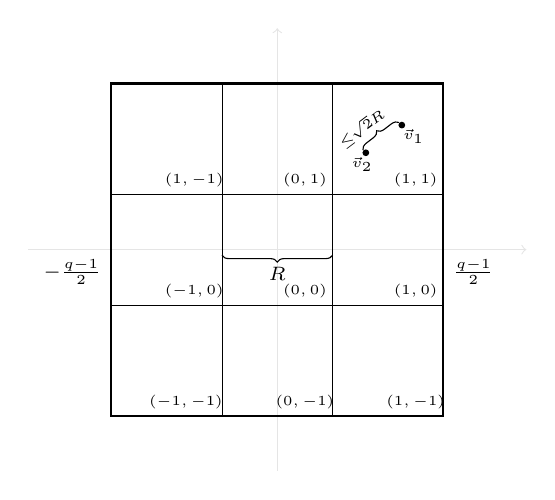
\begin{tikzpicture}
	\draw[gray!20, ->] (-90pt,0) -- (90pt,0);
	\draw[gray!20, ->] (0,-80pt) -- (0,80pt);
	
	 \draw[thick] (-60pt, -60pt) rectangle (60pt, 60pt);
	 \draw (-60pt, 0)  node[below left] {\scriptsize $-\tfrac{q-1}{2}$};
	 \draw (60pt, 0)  node[below right] {\scriptsize $\tfrac{q-1}{2}$};
	 
	 \draw[very thin] (-20pt, -60pt) -- (-20pt, 60pt);
	 \draw[very thin] (20pt, -60pt) -- (20pt, 60pt);
	 \draw[very thin] (-60pt, -20pt) -- (60pt, -20pt);
	 \draw[very thin] (-60pt, 20pt) -- (60pt, 20pt);
	 
	 \draw [decoration={brace, mirror, raise=7pt},
	 		decorate,below=10pt, yshift=5pt](-20pt, 0) -- (20pt, 0) node [black,midway, yshift=-8pt] {\scriptsize $R$};
	 		
	 \filldraw (45pt, 45pt) circle (1pt) node[below right, xshift=-3pt, yshift=2pt] {\tiny $\vvec_1$};
	 \filldraw (32pt, 35pt) circle (1pt) node[below left, xshift=6pt, yshift=2pt] {\tiny $\vvec_2$};
	 
	 \draw [decoration={brace, raise=5pt},
	 	 		decorate,above=10pt, yshift=-3pt, xshift=2pt](32pt, 35pt) -- (45pt, 45pt) node [black,midway, rotate=37, yshift=5pt, xshift=-4pt] {\tiny $ \leq \mkern-6mu \sqrt{2}R$};
	 	 		
	%----------LABELS---------
	\node[draw=none] at (10pt, -15pt){\tiny $(0,0)$};
	\node[draw=none] at (10pt, 25pt){\tiny $(0,1)$};	
	\node[draw=none] at (10pt, -55pt){\tiny $(0,-1)$};
	
	\node[draw=none] at (50pt, 25pt){\tiny $(1,1)$};
	\node[draw=none] at (50pt, -15pt){\tiny $(1,0)$};
	\node[draw=none] at (50pt, -55pt){\tiny $(1,-1)$};
	
	\node[draw=none] at (-30pt, 25pt){\tiny $(1,-1)$};
	\node[draw=none] at (-30pt, -15pt){\tiny $(-1,0)$};
	\node[draw=none] at (-33pt, -55pt){\tiny $(-1,-1)$};
	\end{tikzpicture}
	\caption[Bucketing on a $2$-dimensional $q$-ary lattice]{Bucketing on a $2$-dimensional $q$-ary lattice. Each small cube of length $R$ gets its two-dimensional label. The vectors $\vvec_1$, $\vvec_2$ appear in the same bucket $(1, 1)$ and, hence, the $\ell_2$-norm of their difference is bounded by $\sqrt{2}R$.}
	\label{fig:Bucketing}
\end{figure}

There is one simple trick which greatly improves the running time of the algorithm. We can write our input matrix $\AMat \in \Z_q^{n \times 2n}$ as $\AMat = [\AMat_1 | \AMat_2]$ where $\AMat_i \in \Z_q^{n \times n}$. With high probability, we have that $\AMat_1$ is invertible $\bmod~q$ allowing us to write $\AMat = [\Id_n | \AMat']$ where $\AMat' = \AMat_1^{-1} \AMat_2 \bmod q$. Essentially this procedure brings a $q$-ary code generated by $\AMat$ to a systematic form. It is easy to verify that a basis for $\qLATTp(\AMat)$ is of the form (cf. with the basis $B$ for $\qLat(\AMat\transpose)$ given in Eq.~(\ref{eq:LWEBasis})):
\begin{equation}\label{eq:BasisD}
	\DMat = \begin{pmatrix}
	-\AMat' & q\Id_n \\
	\Id_{n} & 0
	\end{pmatrix}.
\end{equation}


\begin{algorithm}[t]
	\caption{$\appSVP$ on a $q$-ary lattice}
	\label{alg:ApproxSVP}
	\textbf{Input:} $D$ -- a basis for the lattice $\qLATTp(A) \subset \Z_q^{2n}$ defined as in Eq.~(\ref{eq:BasisD}), $\gamma = n^{\cg}$ -- the approximation factor, $\cg>0$ \\
	\textbf{Output:} $L_k$ -- list of vectors from $\qLATTp(A)$ with vectors of norm $\| \vvec \| \leq n^{\cg+\cq/2+1/2}$;
	
	\begin{algorithmic}[1]
		
		\State Set the sieving bounds $R_i$ as $R_1 = n^{\smallo(1)}$ and $R_i = \sqrt{2}^{i-1} R_1$ for $i \geq 2$.
		\State Set the lengths of blocks $d_i$ as in Eq.~(\ref{eq:d_i}) and the boundaries of each block $(l_{i-1}, \ldots, l_i)$ s.t.\ $l_{i}-{l_{i-1}} = d_i$ and $l_k = 1, l_0 = n$.
		
		\Repeat \Comment{Create the list $L_0$}
		\State Choose $\xvec \in \Z_q^{2n}$ s.t.\ $\| [\xvec]_{n+1}^{2n} \|_{\infty} \leq R_1$
		\State $L_0 \gets L_0 \union \{D\xvec \bmod q\} $
		\Until{$L_0$ is large enough}
		
		\State $T \gets \emptyset$ \Comment{Initialize an array $T$ indexed by buckets}
		\ForAll {$i=1 \ldots k$} \label{algline:ForLoop1}
			\ForAll { $\vvec \in L_{i-1}$} \label{algline:ForLoop2}
				\State $b \gets \Big\lfloor \frac{[\vvec]_{l_i}^{l_{i-1}}}{R_i} \Big\rceil$ \Comment Find the bucket for $\vvec\mkern2mu[l_i, \ldots, l_{i-1}]$
				\If{$T[b] = \emptyset$}
					\State $T[b] \gets \vvec$
				\Else
					\State $L_{i} \gets L_{i} \union \{T[b] - \vvec \}$
					\State $T[b] \gets \emptyset$
				\EndIf
			\EndFor
		\EndFor
		\State \Return $L_k$
	\end{algorithmic}
	
	\vspace{10pt}
	
\end{algorithm}

\begin{figure}[H]
	\centering
	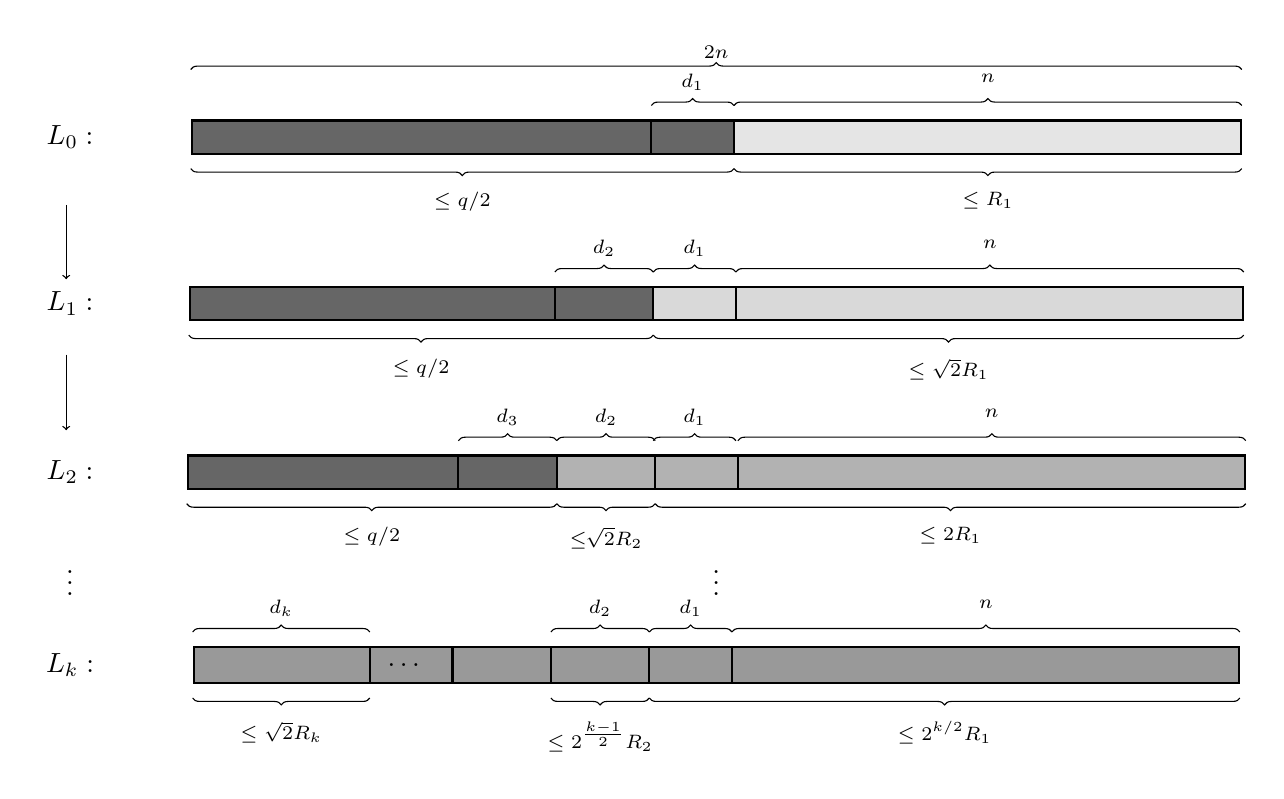
\begin{tikzpicture}[]
	\tikzset{
		List/.style={
			rectangle split, rectangle split horizontal,  
			draw=black, thick,
			%text width=10em,
			inner sep=6pt,
		} 
	}    
	\matrix (m) [row sep=0.8em, column sep=3em]{
		\node[](L0) {$L_0:$}; & 
		\node[List, rectangle split parts=3, name=list, rectangle split part fill={black!60,black!60,black!10}] (list) {
			\nodepart[text width=5.4cm]{one}{}
			\nodepart[text width=0.6cm]{two}
			\nodepart[text width=6cm] {three}};
		
		\draw [decoration={brace, raise=5pt},
		decorate,below=10pt] (list.two split north) -- (list.north east) node [black,midway, yshift=20pt] {\scriptsize $n$}; 
		
		\draw [decoration={brace,raise=5pt},
		decorate,below=10pt](list.one split north) -- (list.two split north) node [black,midway, yshift=20pt] {\scriptsize $d_1$};
		
		\draw [decoration={brace, mirror, raise=5pt},
		decorate,below=10pt](list.two split south) -- (list.south east) node [black,midway, yshift=-10pt] {\scriptsize $\leq R_1$};
		
		\draw [decoration={brace, mirror, raise=5pt},
		decorate,below=10pt](list.south west) -- (list.two split south) node [black,midway, yshift=-10pt] {\scriptsize $\leq q/2$};
		\draw [decoration={brace,raise=18pt},
		decorate,below=10pt](list.north west) -- (list.north east) node [black,midway,yshift=30pt] {\scriptsize $2n$};\\[-1ex]
		%---------------------------------------  
		\node[](L1) {$L_1:$}; & 
		\node[List, rectangle split parts=4, name=list2, rectangle split part fill={black!60,black!60,black!15,black!15}] (list2) {
			\nodepart[text width=4.2cm]{one}{}
			\nodepart[text width=0.8cm]{two}
			\nodepart[text width=0.6cm] {three}
			\nodepart[text width=6cm] {four}};
		
		\draw [decoration={brace,raise=5pt},
		decorate,below=10pt](list2.three split north) -- (list2.north east) node [black,midway, yshift=20pt] {\scriptsize $n$}; 
		
		\draw [decoration={brace,raise=5pt},
		decorate,below=10pt](list2.two split north) -- (list2.three split north) node [black,midway, yshift=20pt] {\scriptsize $d_1$};
				
				
		\draw [decoration={brace, mirror, raise=5pt},
		decorate,below=10pt](list2.two split south) -- (list2.south east) node [black,midway, yshift=-10pt] {\scriptsize $\leq \sqrt{2}R_1$};

		
		\draw [decoration={brace,raise=5pt},
		decorate,below=10pt](list2.one split north) -- (list2.two split north) node [black,midway, yshift=20pt] {\scriptsize $d_2$};
		
		\draw [decoration={brace, mirror, raise=5pt},
		decorate,below=10pt](list2.south west) -- (list2.two split south) node [black,midway, yshift=-10pt] {\scriptsize $\leq q/2$};\\ [-1ex]
		
		%---------------------------------------  
		\node[](L2) {$L_2:$}; & 
		\node[List, rectangle split parts=5, name=list3, rectangle split part fill={black!60,black!60,black!30,black!30,black!30}] (list3) {
					\nodepart[text width=3.0cm]{one}{}
					\nodepart[text width=0.8cm]{two}
					\nodepart[text width=0.8cm]{three}
					\nodepart[text width=0.6cm] {four}
					\nodepart[text width=6cm] {five}};
				
		\draw [decoration={brace,raise=5pt},
		decorate,below=10pt](list3.four split north) -- (list3.north east) node [black,midway, yshift=20pt] {\scriptsize $n$}; 
				
		\draw [decoration={brace,raise=5pt},
		decorate,below=10pt](list2.two split north) -- (list2.three split north) node [black,midway, yshift=20pt] {\scriptsize $d_1$};
								
		\draw [decoration={brace, mirror, raise=5pt},
		decorate,below=10pt](list3.three split south) -- (list3.south east) node [black,midway, yshift=-10pt] {\scriptsize $\leq 2 R_1$};
		
		\draw [decoration={brace,raise=5pt},
		decorate,below=10pt](list3.two split north) -- (list3.three split north) node [black,midway, yshift=20pt] {\scriptsize $d_2$};
				
		\draw [decoration={brace, mirror, raise=5pt},
		decorate,below=10pt](list3.two split south) -- (list3.three split south) node [black,midway, yshift=-10pt] {\scriptsize $\leq  \mk \sqrt{2}R_2$};
		
		\draw [decoration={brace,raise=5pt},
		decorate,below=10pt](list3.one split north) -- (list3.two split north) node [black,midway, yshift=20pt] {\scriptsize $d_3$};
		
		\draw [decoration={brace, mirror, raise=5pt},
		decorate,below=10pt](list3.south west) -- (list3.two split south) node [black,midway, yshift=-10pt] {\scriptsize $\leq q/2$};\\ [-3ex]
		
		\node[] (vd) {$\vdots$}; &
		\node[]{$\vdots$}; \\ [-3ex]
		%---------------------------------------  
		
		\node[](Lk) {$L_k:$}; & 
		\node[List, rectangle split parts=6, name=list4,rectangle split part fill={black!40,black!40,black!40,black!40,black!40,black!40}] (list4) {
			\nodepart[text width=1.8cm]{one}{}
			\nodepart[text width=0.6cm]{two}{$\ldots$}
			\nodepart[text width=0.8cm]{three}
			\nodepart[text width=0.8cm] {four}
			\nodepart[text width=0.6cm] {five}
			\nodepart[text width=6cm] {six}};
		
		\draw [decoration={brace,raise=5pt},
		decorate,below=10pt](list4.five split north) -- (list4.north east) node [black,midway, yshift=20pt] {\scriptsize $n$}; 
		
		\draw [decoration={brace,raise=5pt},
		decorate,below=10pt](list4.four split north) -- (list4.five split north) node [black,midway, yshift=20pt] {\scriptsize $d_1$};
		
		\draw [decoration={brace,mirror, raise=5pt},
		decorate,below=10pt](list4.four split south) -- (list4.south east) node [black,midway, yshift=-10pt] {\scriptsize $ \leq 2^{k/2} R_1$};
		
		\draw [decoration={brace,raise=5pt},
		decorate,below=10pt](list4.three split north) -- (list4.four split north) node [black,midway, yshift=20pt] {\scriptsize $d_2$};
				
		\draw [decoration={brace, mirror, raise=5pt},
		decorate,below=10pt](list4.three split south) -- (list4.four split south) node [black,midway, yshift=-10pt] {\scriptsize $\leq 2^{\tfrac{k-1}{2}} R_2$};
		
		\draw [decoration={brace, raise=5pt},
		decorate,below=10pt](list4.north west) -- (list4.one split north) node [black,midway, yshift=20pt] {\scriptsize $d_k$};
		
		\draw [decoration={brace, mirror, raise=5pt},
		decorate,below=10pt](list4.south west) -- (list4.one split south) node [black,midway, yshift=-10pt] {\scriptsize $\leq \sqrt{2} R_k$};
		
		%\draw [decoration={brace,raise=5pt},
		%decorate,below=10pt](list4.four split north) -- (list4.north east) node [black,midway, yshift=20pt] {\scriptsize $l_k$};
		 \\
	};		
	%\draw[->, thick] ([yshift=2cm]L0) -- (L1);
	\draw[transform canvas={scale=0.6, xshift=-140pt, yshift=30pt}, ->, thick] (L0) -- (L1);
	\draw[transform canvas={scale=0.6, xshift=-140pt, yshift=0pt}, ->, thick] (L1) -- (L2);
	\end{tikzpicture}
	\caption[$\appSVP$ on a $q$-ary lattice]{ Visualization of Alg.~\ref{alg:ApproxSVP}. Each horizontal rectangle represents a form of a vector from the input-list $L_{i-1}$ on step $i$ for $i=1, 2, 3$ (counting from top to bottom) and a vector from the output list $L_k$ (the lower-most rectangle). The vectors are of dimension $2n$. Labels of the upper brackets denote the length of the blocks, while labels of the lower brackets denote the $\ell_{\infty}$-norm of the corresponding block. The darker the shading for a block is, the larger its $\ell_{\infty}$-norm. Note that the algorithm chooses the bounds $R_i$ s.t.\ the $\ell_{\infty}$-norm on the previous (right-hand side) blocks is the same as on the currently considered block (i.e.\ $R_i = \sqrt{2}R_{i-1}$). With such a choice, the contribution to the expected norm of vectors from the final list $L_k$ is equal from each block.}
	\label{fig:appSVPAlg}
\end{figure}

Now we use this basis to generate the lattice-vectors to perform the initial search. We will choose $\xvec  = (x_1, \ldots, x_n, x_{n+1}, x_{2n}) \in \Z_q^{2n}$ and produce vectors
\[
D \xvec \bmod q = (y_1,  \ldots,  y_n,  x_{n+1}, \ldots, x_{2n})^{\transpose}.
\]

This way we can already bound the $\ell_{\infty}$-norm of the vectors on the right-most $n$ coordinates by choosing $(x_{n+1}, \ldots, x_n)$, say, less than $R_1$ (as if we would have already bucketed the right-hand side). We put vectors of this form in our starting list $L_0$. Elements from this list allow us to perform our `cube-bucketing' of the remaining left $n$-coordinates only as opposed to $2n$. 

Our $\appSVP$ algorithm can be easily formulated as an algorithm for a $k$-List problem in the sense of Def.~\ref{def:kList}: given $2^k$ copies of $L_0$, find $k$-tuples $(\vvec_1, \ldots, \vvec_k) \in L_0 \times \ldots \times L_0$, s.t. $\| \vvec_1 \pm \ldots \pm \vvec_k \| \leq n^{\cg+\cq/2+1/2}$.  On Step 1, the algorithm groups $2^k$ lists $L_0$ into $2^{k-1}$ pairs of lists and from each list-pair $(L_0, L_0)$ searches for $(\vvec_i, \vvec_{i+1})$ that appear in the same `bucket' on their first $d_1$ coordinates. Once found, $(\vvec_i - \vvec_{i+1})$ is put into $L_1$. At the end, we have $2^{k-1}$ copies of the list $L_1$. The algorithm terminates with one copy of $L_k$ that contains a vector with bounded $\ell_\infty$-norm. By setting $k$ appropriately, we can guarantee that the Euclidean length of this vector is bounded as desired.

Below we describe the algorithm in pseudo-code and in Fig.~\ref{fig:appSVPAlg}. The array $T$ in pseudo-code serves as a look-up table: on step $i$, it is indexed by $d_i$-dimensional vectors (buckets) $b$ and whenever we find a vector $\vvec$ s.t. $\Big\lfloor \frac{[\vvec_1]_1^{d_1}}{R_1} \Big\rceil = b$, we look up whether $T[b]$ is empty or not. In the latter case, the collision is found and a new vector is added to $L_{i}$. 

\subsection{Analysis} \label{subsec:qAryAnalysis}

It is reasonable to assume that the above algorithm for $\appSVP$ on a $q$-ary lattice, as all known \BKW-type algorithms for \LWE, has both running time and memory complexity of the form $2^{(\const+\smallo(1) )n}$ for some constant $\const$. The goal of this section is to determine $\const$ as a function of input parameters: $\cg$, where $\gamma = \bigO(n^{\cg})$, and $\cq$, where $q = \bigO(n^{\cq})$. We consider average-case instances, and our analysis will show the \emph{expected} running time and memory.

Let us elaborate more on the running-time/memory trade-off achieved by the algorithm. Recall that on step $i$, one entry of table $T$ represents one bucket which is one of the small cubes $[-R_i/2, R_i/2]^{\ell_i}$ inside a large cube $[-\frac{q-1}{2}, \frac{q-1}{2}]^{\ell_i}$ (see Fig.~\ref{fig:Bucketing}). We expect to have all entries of $T$ be filled after we have bucketed ($\#$buckets)-many lattice vectors from $L_{i-1}$ (here we use the fact that elements from $L_{i-1}$, subjected on block $\ell_i$, are uniformly distributed in $[-\frac{q-1}{2}, \frac{q-1}{2}]^{\ell_i}$). Hence, after bucketing ($2 \cdot \#$buckets)-many lattice vectors from $L_{i-1}$, we expect to put ($\#$buckets)-many lattice vectors into $L_i$. Overall, the lists get shorter by at least a factor of $2$ per level. After $k$ levels, we expect $|L_k| = \TLandau(2^{-k} |L_0|)$. 

The analysis below reveals $k = \TLandau(\log n)$, and hence, the output list $L_k$ is expected to be only $\poly(n)$-times shorter than the initial list $L_0$. We shall see in the proof that the number of buckets on each level will be exponential in $n$, hence, to find even one collision on step $i$, we need exponentially many lattice vectors in the list $L_{i-1}$. So we ignore $\poly(n)$-factors coming from the fact that we lose approximately half of the list on each step. Also, the amount of computations we perform per bucket is only $\bigO(n)$ as we add up two $n$-dimensional vectors. Thus, both the expected running time and memory complexity are equal (up to $\poly(n)$-factors) to the number of buckets. Exactly the same arguments apply to \BKW algorithms for \LWE.

Intuitively, it would be beneficial to take the number of steps $k$ large as it leads to shorter block-lengths $\ell_i$'s which, in turn, speeds up the collision-finding. However, we have to set $k$ as low as $k = \TLandau(\log n)$ where the constant in $\TLandau$-notation will ultimately depend on $\cg$ and $\cq$. This bound comes from the fact that each time we perform addition of two vectors that happen to lie in the same bucket, the $\ell_{\infty}$-norm of the resulting vector on \emph{already considered} blocks $\ell_1, \ldots, \ell_{i-1}$ increases (on average) by a factor of $\sqrt{2}$. So shortening the $\ell_{\infty}$-norm from $q$ down to $\sqrt{2}R_i$ on a block enlarges the $\ell_{\infty}$-norm of the vector by $\sqrt{2}$ on the right-hand side blocks. This growth is depicted in Fig.~\ref{fig:appSVPAlg}. At the end, on the coordinate block $[d_{i-1}, \ldots, d_{i}]$ of length $\ell_i$, we have $\| [\vvec\mkern3mu]_{d_i}^{d_{i-1}} \|_{\infty} \leq 2^{\frac{k-i+1}{2}} R_i $ for $\vvec \in L_k$. Hence our choice for $k$ is restricted by the upper bound of the Euclidean length of $\vvec$ we should output. This situation should be compared with the error-growth in the \BKW algorithm for \LWE that puts a bound on $k$ of the same order.

%The number of buckets on step $i$ is given by the fraction of the two volumes of cubes $\#$buckets$= \frac{\vol([-\frac{q-1}{2}, \frac{q-1}{2}]^{\ell_i})}{\vol([-R_i/2, R_i/2]^{\ell_i})} = (\frac{q}{R_i})^{\ell_i}$.

In the proof below we show how to set the block-lengths $\ell_i$'s, the $\ell_\infty$-norm bounds $R_i$'s, and the number of steps $k$.
\begin{thm} \label{thm:appSVP}
	Algorithm~\ref{alg:ApproxSVP} on input (1) a lattice-basis $\DMat \in \Z_q^{2n \times 2n}$ as in Eq.~(\ref{eq:BasisD}) for the lattice $\qLATTp(A)$ with $q = \bigO(n^{\cq})$ and (2) an approximation factor $\gamma = \bigO(n^{\cg})$, outputs a vector $\vvec \in \qLATTp(A)$ of length $\|\vvec \| \leq n^{\cg+\cq/2 + 1/2}$ in expected time $T(\appSVP)=2^{(\const+\smallo(1)) n}$, where
	\begin{equation} \label{eq:AppSVPRT}
		\const = \tfrac{1}{2 \ln \big( \frac{\cq}{\cq/2-\cg} \big)}.
	\end{equation}
\end{thm}

\begin{proof}
	The expected running time to fill up all the buckets on step $i$ and, thus, to create the list $L_{i}$ is determined by the number of buckets or, equivalently, the number of $\ell_i$-dimensional cubes $[-R_i/2, R_i/2]^{\ell_i}$ that `fit' inside the large cube $[-\frac{q-1}{2}, \frac{q-1}{2}]$. This number is given by the fraction of the two volumes:
	\[
		\E[\#\text{buckets on level } i]= \frac{\vol([-\frac{q-1}{2}, \frac{q-1}{2}]^{d_i})}{\vol([-R_i/2, R_i/2]^{d_i})} = \TLandau \Big( \Big(\frac{q}{R_i}\Big)^{d_i}\Big).	
	\]
	This is (up to $\poly(n)$-factors) the expected running time of the inner for-loop (line \ref{algline:ForLoop2}).
	As we show below, the number of steps $k$ will be of size $k = \TLandau(\log n)$ and hence, the outer for-loop on line \ref{algline:ForLoop1} in Alg.~\ref{alg:ApproxSVP} contributes to the running time only by a $\poly(n)$-factor. 
	
	Thus, asymptotically, we have $\big(\frac{q}{R_i}\big)^{d_i} = 2^{\const n}$, from where it follows that 
	\begin{equation} \label{eq:d_i}
		d_i = \frac{\const n}{\log q - \log R_i}.
	\end{equation}
	
	Additionally, we have $\sum_{i=1}^k d_i = n$. We shall conclude on $\const$ from these two equations.
	
	But before doing that let us get an upper-bound for $k$. The expected length of vector $\vvec$ in the list $L_k$ is upper-bounded as $\| \vvec \| \leq \sqrt{2 R_k^2 d_k + 4 R_{k-1}^2 d_{k-1} + \ldots + 2^{k-1} R_2^2 d_2 + 2^k R_1^2 d_1 + 2^k R_1^2 n}$. It is easy to verify (see also Fig.~\ref{fig:appSVPAlg}) that if we set $R_{i+1} = \sqrt{2} R_i$, the first $k$ summands in our bound on $\|\vvec \|$ contribute to the total sum equally. Finally, we obtain $\| \vvec \| \leq \sqrt{2 2^{k} R_1^2 n}$. This bound should be less than $n^{\cg +\cq/2 +1/2}$. If we set the first bound $R_1$ as small as $R=n^{\smallo(1)}$, the inequality $\sqrt{2 2^{k} R_1^2 n} \leq n^{\cg +\cq/2 +1/2}$ leads to $k \leq 2 (\cg+\cq/2 + \smallo(1)) \log n$. We take the upper bound as the value for $k$.  
	
	Since we set $R_i = \sqrt{2}^{i-1} R_1$, we now can compute the sum $\sum_{i=1}^k d_i$ as
	\[	
	\sum_{i=1}^{k} \frac{\const n}{\log \tfrac{q}{ R_1} - \tfrac{1}{2}(i-1)} \leq  \int\limits_{i=0}^{k-1} \frac{\const n  \d i}{\log (\tfrac{q}{ R_1}) - \tfrac{1}{2}i} = - 2\const n \Big( \ln(\log \tfrac{q}{ R_1} - \tfrac{1}{2}i) \Big|_0^{k-1} \Big) = 2\const n \ln \Big( \frac{\log \tfrac{q}{ R_1}}{\log \tfrac{q}{ R_1} - \tfrac{1}{2} (k-1)} \Big).
	\]
	The error that comes from approximating the sum by the integral contributes to the $\smallo(1)$-term in the exponent.
	From the facts that all $d_i$'s sum up to $n$, $k=2 (\cg+\cq/2)\log n$, and $R_1 = n^{\smallo(1)}$, we obtain
	\[\const = \frac{1}{2 \ln \big( \tfrac{\cq}{\cq/2-\cg} \big)} +\smallo(1).\]
	\vspace{-13pt}
\end{proof}

\begin{remark}\label{rmk:Linm}
	From the proof above, it is easy to deduce that for $m=\cm \cdot n$, $\cm = \TLandau(1)$
 	\[
		\const = \frac{\cm -1 }{2 \ln \big( \frac{\cq}{\cq (1-1/\cm) - \cg} \big)}.
	\]
\end{remark}
We conclude the discussion on the algorithm with a couple of remarks.
	\begin{itemize}
		\setlength{\itemsep}{0pt}
		  \setlength{\parskip}{0pt}
		\item \textbf{Connection to \BKZ algorithms.} An important property of our $q$-ary lattice $\qLATTp(A)$ we are exploiting in this algorithm is the \emph{orthogonal} sub-lattice $q\Id_n \subset \qLATTp(A)$. We can view each bucketing step as projection of vectors onto the $q$-ary vectors $\{(q, 0, \ldots, 0), \ldots (0, 0, \ldots, q)\}$ first, then performing the summation, and finally `lifting' the result. Since the sub-lattice is orthogonal, the lifting is simply a coordinate-wise $\bmod q$ operation. This allows us not to worry about the $\ell_{\infty}$-norm on the left-most coordinates where the bucketing was not yet performed as we implicitly assume the $\bmod~q$ operation. The algorithm can be thought of as a special kind of $\BKZ$-reduction, where, instead of projecting on short and non-orthogonal vectors, we project on long but orthogonal vectors. Also, as opposed to a $\BKZ$ algorithm where the block-size is fixed to $\beta$, our $d_i$'s differ. Further, our blocks do not intersect similar to the $\BKZ$ slide-reduction.\\
		\item \textbf{Connection to \BKW algorithms}. As we already mentioned, the presented algorithm is a re-formulation of the \BKW algorithms of \cite{C:KirFou15, C:GuoJohSta15} to $\appSVP$. The fact that we can `save' half of the dimension, $n$, by switching to the systematic form of the generator matrix $\AMat$ is no surprise: solving \LWE directly with \BKW (not via lattices) does not have this additional $n$ at all. 
	\end{itemize}


\subsection{An improved algorithm for $\appSVP$ on a $q$-ary lattice} \label{subsec:qAryAlgImproved}

In this section we present an improved algorithm for $\appSVP$ on a $q$-ary lattice. The improvement is in the constant $\const$. We introduce a new constant $\eps$ in the algorithm and $\const$ will depend on it. Namely, when $0<\eps<1/4$, the algorithm achieves a smaller value for $\const$, and when $\eps=0$, it is Algorithm~\ref{alg:ApproxSVP} from the previous section.

The gain comes from the following two changes. First, we do not only perform bucketing on `new' coordinates on the left part (i.e.\ on coordinates with $\ell_{\infty}$-norm less than $q/2$), but also on already considered coordinates on the right part, i.e.\ on blocks in-between the $n\th$ and the $2n\th$ coordinates. 

Second, and more importantly, we reduce the growth of the block-bounds $R_i$. Recall that in the previous algorithm, we had $R_{i+1} = \sqrt{2}R_i$, where the $\sqrt{2}$ comes from the average $\ell_{\infty}$-norm of the sum of two vectors whose $\ell_{\infty}$-norm is $R_i$. This choice balanced the $\ell_{\infty}$-norm on the block $d_i$ with the $\ell_{\infty}$-norm on all the previous blocks $d_{i-1}, \ldots, d_1$.
Now, we set $R_{i+1} = 2^{1/2 - \eps}R_i$ for some $\eps>0$. The fact that we set $\eps>0$ is justified by our additional bucketing on the right part which requires another choice of $R_i$'s  to balance the norms between the blocks. When compared with the previous algorithm, the expected length of a vector from $L_i$ when we perform this new bucketing is shorter, and since the final length is fixed to $n^{\cg+\cq/2+1/2}$, we can choose larger (by a constant factor) $k$. From the analysis of the previous algorithm, it follows that any constant improvement for $k$ results in smaller $\const$ (see the proof of Thm.~\ref{thm:appSVP}).

Let us describe the algorithm in more detail. The initial list $L_0$ is created in the same way as in Algorithm~\ref{alg:ApproxSVP}: we sample a vector $\xvec \in \Z_q^{2n}$ with the right-most $n$ coordinates bounded by $R_1$. The remaining $n$ left-most coordinates are divided into $k$ blocks of length $d_i$. Note that we can `mirror' this partition to the right-most $n$ coordinates w.r.t. the `middle' $n\th$ coordinate. Let us denote the bounds of the $i\th$ block of length $d_i$ as $[l_{i},\ldots, l_{i-1}]$ for the left part (i.e. $[l_{i-1},\ldots, l_{i}] \in [1, \ldots, n]$) and $[r_{i-1}, \ldots, r_{i}]$ for the right part (i.e.\ $[r_{i-1}, \ldots, r_{i}]\in [n+1, \ldots, 2n]$, see Fig.~\ref{fig:appSVPAlgImproved}).

\begin{algorithm}[t]
	\caption{$\appSVP$ on a $q$-ary lattice}
	\label{alg:ApproxSVPImprived}
	\textbf{Input:} $D$ -- a basis for the lattice $\qLATTp(A) \subset \Z_q^{2n}$ defined as in Eq.~(\ref{eq:BasisD}), $\gamma = n^{\cg}$ -- the approximation factor, $\cg=\TLandau(1)$ \\
	\textbf{Output:} $L_k$ -- list of vectors from $\qLATTp(A)$ with vectors of norm $\| \vvec \| \leq n^{\cg+\cq/2+1/2}$;
	
	\begin{algorithmic}[1]
		
		\State Set the sieving bounds $R_i$ as $R_1 = n^{\smallo(1)}$ and ${\color{blue}R_i = 2^{(1/2-\eps)(i-1)} R_1}$ for $i \geq 2$.
		\State Set the lengths of blocks $d_i$ as in Eq.~(\ref{eq:d_iImp}) together with the corresponding boundaries of the {\color{blue}left-hand side} blocks $(l_i, \ldots, l_{i-1})$ and of the {\color{blue}right-hand side} blocks $(r_{i-1}, \ldots, r_i)$ s.t.\ $l_{i}-{l_{i-1}} = r_{i-1} -r_i  = d_i$, and $l_k = 2n, l_0 = r_0 = n, r_k = 2n$.
		
		\Repeat \Comment{Create the list $L_0$}
		\State Choose $\xvec \in \Z_q^{2n}$ s.t.\ $\| [\xvec]_{n+1}^{2n} \|_{\infty} \leq R_1$
		\State $L_0 \gets L_0 \union \{D\xvec \bmod q\} $
		\Until{$L_0$ is large enough} 
		
		\State $T \gets \emptyset$ \Comment{Initialize table $T$ indexed by buckets}
		\ForAll {$i=1 \ldots k$} 
		\ForAll { $\vvec \in L_{i-1}$} 
		\State ${\color{blue} b \gets \Big\lfloor \frac{[\vvec\mkern2mu]_{l_i}^{l_{i-1}} [\vvec\mkern2mu]_{r_{i-1}}^{r_i}}{R_i} \Big\rceil}$ \Comment Find the bucket for $\vvec[l_i, \ldots, l_{i-1}, r_{i-1}, \ldots r_i]$
		\If{$T[b] = \emptyset$}
		\State $T[b] \gets \vvec$
		\Else
		\State $L_{i} \gets L_{i} \union \{T[b] - \vvec \}$
		\State $T[b] \gets \emptyset$
		\EndIf
		\EndFor
		\EndFor
		\State \Return $L_k$
	\end{algorithmic}
\end{algorithm}
\begin{figure}[H]
	\centering
	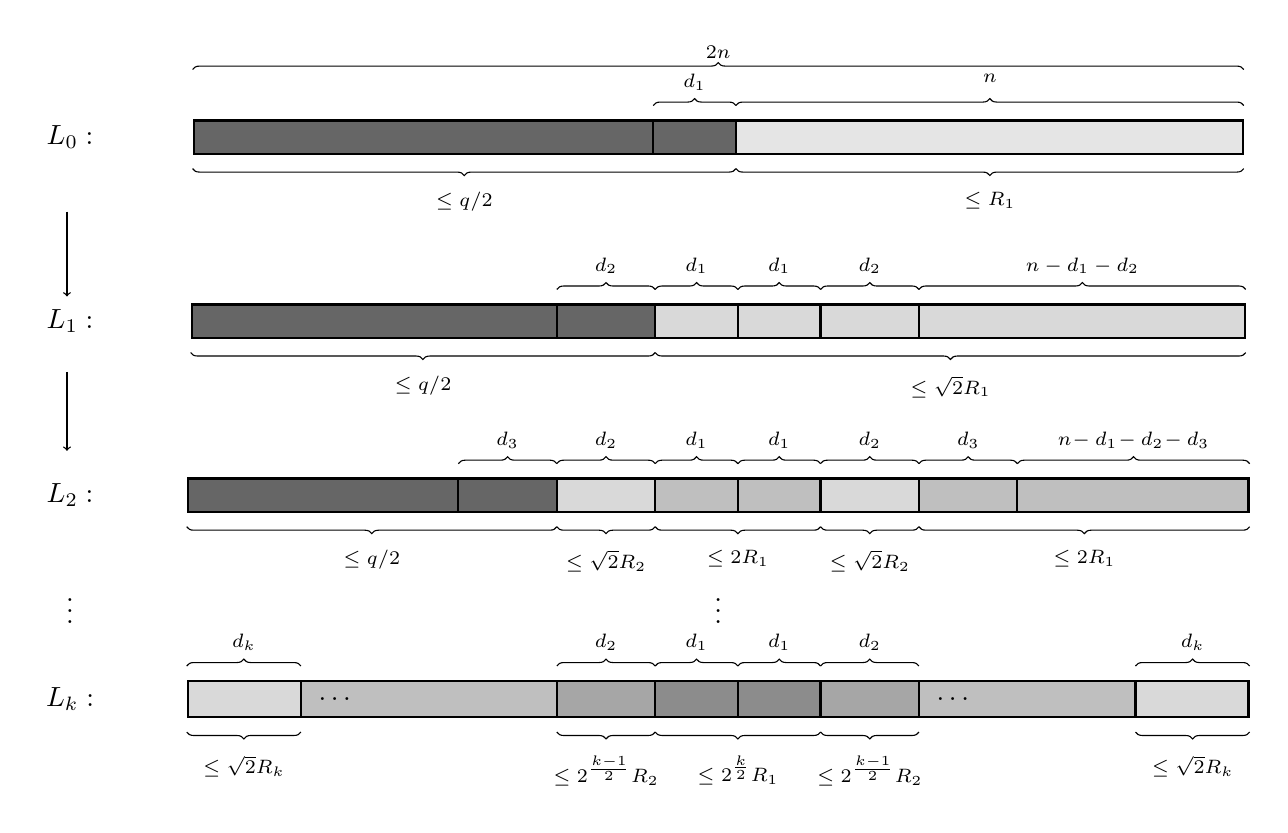
\begin{tikzpicture}[]
	\tikzset{
		List/.style={
			rectangle split, rectangle split horizontal,  
			draw=black, thick,
			%text width=10em,
			inner sep=6pt,
		} 
	}    
	%\draw[gray!30, ->] (34pt,-130pt) -- (34pt,130pt);
	\matrix (m) [row sep=1em, column sep=3em]{
		\node[](L0) {$L_0:$}; & 
		\node[List, rectangle split parts=3, name=list, rectangle split part fill={black!60,black!60,black!10}] (list) {
			\nodepart[text width=5.4cm]{one}{}
			\nodepart[text width=0.6cm]{two}
			\nodepart[text width=6cm] {three}};
		
		\draw [decoration={brace, raise=5pt},
		decorate,below=10pt] (list.two split north) -- (list.north east) node [black,midway, yshift=20pt] {\scriptsize $n$}; 
		
		\draw [decoration={brace,raise=5pt},
		decorate,below=10pt](list.one split north) -- (list.two split north) node [black,midway, yshift=20pt] {\scriptsize $d_1$};
		
		\draw [decoration={brace, mirror, raise=5pt},
		decorate,below=10pt](list.two split south) -- (list.south east) node [black,midway, yshift=-10pt] {\scriptsize $\leq R_1$};
		
		\draw [decoration={brace, mirror, raise=5pt},
		decorate,below=10pt](list.south west) -- (list.two split south) node [black,midway, yshift=-10pt] {\scriptsize $\leq q/2$};
		\draw [decoration={brace,raise=18pt},
		decorate,below=10pt](list.north west) -- (list.north east) node [black,midway,yshift=30pt] {\scriptsize $2n$};\\
		%---------------------------------------  
		\node[](L1) {$L_1:$}; & 
		\node[List, rectangle split parts=6, name=list2, rectangle split part fill={black!60,black!60,black!15,black!15}] (list2) {
			\nodepart[text width=4.2cm]{one}{}
			\nodepart[text width=0.8cm]{two}
			\nodepart[text width=0.6cm] {three}
			\nodepart[text width=0.6cm] {four}
			\nodepart[text width=0.8cm] {five}
			\nodepart[text width=3.7cm] {six}};
		
		\draw [decoration={brace,raise=5pt},
		decorate,below=10pt](list2.five split north) -- (list2.north east) node [black,midway, yshift=20pt] {\scriptsize $n-d_1-d_2$};
		
		\draw [decoration={brace,raise=5pt},
		 decorate,below=10pt](list2.three split north) -- (list2.four split north) node [black,midway, yshift=20pt] {\scriptsize $d_1$};
		
		\draw [decoration={brace,raise=5pt},
		decorate,below=10pt](list2.two split north) -- (list2.three split north) node [black,midway, yshift=20pt] {\scriptsize $d_1$};
		
		
		\draw [decoration={brace, mirror, raise=5pt},
		decorate,below=10pt](list2.two split south) -- (list2.south east) node [black,midway, yshift=-10pt] {\scriptsize $\leq \sqrt{2}R_1$};
		
		
		\draw [decoration={brace,raise=5pt},
		decorate,below=10pt](list2.one split north) -- (list2.two split north) node [black,midway, yshift=20pt] {\scriptsize $d_2$};
		
		\draw [decoration={brace,raise=5pt},
		decorate,below=10pt](list2.four split north) -- (list2.five split north) node [black,midway, yshift=20pt] {\scriptsize $d_2$};
		
		\draw [decoration={brace, mirror, raise=5pt},
		decorate,below=10pt](list2.south west) -- (list2.two split south) node [black,midway, yshift=-10pt] {\scriptsize $\leq q/2$};\\ [-1ex]
		
		%---------------------------------------  
		\node[](L2) {$L_2:$}; & 
		\node[List, rectangle split parts=8, name=list3, rectangle split part fill={black!60,black!60,black!15,black!25,black!25,black!15,black!25}] (list3) {
			\nodepart[text width=3.0cm]{one}{}
			\nodepart[text width=0.8cm]{two}
			\nodepart[text width=0.8cm]{three}
			\nodepart[text width=0.6cm]{four}
			\nodepart[text width=0.6cm]{five}
			\nodepart[text width=0.8cm]{six}
			\nodepart[text width=0.8cm]{seven}
			\nodepart[text width=2.5cm]{eight}};
		
		\draw [decoration={brace,raise=5pt},
		decorate,below=10pt](list3.seven split north) -- (list3.north east) node [black,midway, yshift=20pt] {\scriptsize $n\mkern-3mu-d_1\mkern-3mu-d_2\mkern-3mu-d_3$}; 
		
		\draw [decoration={brace, mirror, raise=5pt},
		decorate,below=10pt](list3.six split south) -- (list3.south east) node [black,midway, yshift=-10pt] {\scriptsize $ \leq 2 R_1$};
		
		\draw [decoration={brace,raise=5pt},
		decorate,below=10pt](list3.six split north) -- (list3.seven split north) node [black,midway, yshift=20pt] {\scriptsize $d_3$};
		
		\draw [decoration={brace,raise=5pt},
		decorate,below=10pt](list3.five split north) -- (list3.six split north) node [black,midway, yshift=20pt] {\scriptsize $d_2$};
		
		\draw [decoration={brace, mirror, raise=5pt},
		decorate,below=10pt](list3.five split south) -- (list3.six split south) node [black,midway, yshift=-10pt] {\scriptsize $\leq \sqrt{2}R_2$};
		
		\draw [decoration={brace,raise=5pt},
		decorate,below=10pt](list3.four split north) -- (list3.five split north) node [black,midway, yshift=20pt] {\scriptsize $d_1$};
		
		\draw [decoration={brace,raise=5pt},
		decorate,below=10pt](list3.three split north) -- (list3.four split north) node [black,midway, yshift=20pt] {\scriptsize $d_1$};
		
		\draw [decoration={brace, mirror, raise=5pt},
		decorate,below=10pt](list3.three split south) -- (list3.five split south) node [black,midway, yshift=-10pt] {\scriptsize $\leq 2
		R_1$};		
		
		
		\draw [decoration={brace,raise=5pt},
		decorate,below=10pt](list3.two split north) -- (list3.three split north) node [black,midway, yshift=20pt] {\scriptsize $d_2$};
		
		\draw [decoration={brace, mirror, raise=5pt},
		decorate,below=10pt](list3.two split south) -- (list3.three split south) node [black,midway, yshift=-10pt] {\scriptsize $\leq \sqrt{2}R_2$};
		
		\draw [decoration={brace,raise=5pt},
		decorate,below=10pt](list3.one split north) -- (list3.two split north) node [black,midway, yshift=20pt] {\scriptsize $d_3$};
		
		\draw [decoration={brace, mirror, raise=5pt},
		decorate,below=10pt](list3.south west) -- (list3.two split south) node [black,midway, yshift=-10pt] {\scriptsize $\leq q/2$};\\ [-3ex]
		
		\node[] (vd) {$\vdots$}; &
		\node[]{$\vdots$}; \\ [-3ex]
		%---------------------------------------  
		
		\node[](Lk) {$L_k:$}; & 
		\node[List, rectangle split parts=8, name=list4, rectangle split part fill={black!15,black!25,black!35,black!45,black!45,black!35,black!25,black!15}] (list4) {
			\nodepart[text width=1.0cm]{one}{}
			\nodepart[text width=2.8cm]{two}{\ldots}
			\nodepart[text width=0.8cm]{three}
			\nodepart[text width=0.6cm]{four}
			\nodepart[text width=0.6cm]{five}
			\nodepart[text width=0.8cm]{six}
			\nodepart[text width=2.3cm]{seven}{\ldots}
			\nodepart[text width=1.0cm]{eight}};
		
		\draw [decoration={brace,raise=5pt},
		decorate,below=10pt](list4.seven split north) -- (list4.north east) node [black,midway, yshift=20pt] {\scriptsize $d_k$}; 
		
		\draw [decoration={brace, mirror, raise=5pt},
		decorate,below=10pt](list4.seven split south) -- (list4.south east) node [black,midway, yshift=-10pt] {\scriptsize $\leq \sqrt{2}R_k$};
		
		\draw [decoration={brace,raise=5pt},
		decorate,below=10pt](list4.five split north) -- (list4.six split north) node [black,midway, yshift=20pt] {\scriptsize $d_2$};
		
		\draw [decoration={brace, mirror, raise=5pt},
		decorate,below=10pt](list4.five split south) -- (list4.six split south) node [black,midway, yshift=-10pt] {\scriptsize $ \leq 2^{\tfrac{k-1}{2}} R_2$};
		
		\draw [decoration={brace,raise=5pt},
		decorate,below=10pt](list4.four split north) -- (list4.five split north) node [black,midway, yshift=20pt] {\scriptsize $d_1$};
		
		\draw [decoration={brace,raise=5pt},
		decorate,below=10pt](list4.three split north) -- (list4.four split north) node [black,midway, yshift=20pt] {\scriptsize $d_1$};
		
		\draw [decoration={brace, mirror, raise=5pt},
		decorate,below=10pt](list4.three split south) -- (list4.five split south) node [black,midway, yshift=-10pt] {\scriptsize $ \leq 2^{\tfrac{k}{2}} R_1$};
		
		\draw [decoration={brace,raise=5pt},
		decorate,below=10pt](list4.two split north) -- (list4.three split north) node [black,midway, yshift=20pt] {\scriptsize $d_2$};
		
		\draw [decoration={brace, mirror, raise=5pt},
		decorate,below=10pt](list4.two split south) -- (list4.three split south) node [black,midway, yshift=-10pt] {\scriptsize $ \leq 2^{\tfrac{k-1}{2}} R_2$};
		
		\draw [decoration={brace, raise=5pt},
		decorate,below=10pt](list4.north west) -- (list4.one split north) node [black,midway, yshift=20pt] {\scriptsize $d_k$};
		
		\draw [decoration={brace, mirror, raise=5pt},
		decorate,below=10pt](list4.south west) -- (list4.one split south) node [black,midway, yshift=-10pt] {\scriptsize $\leq \sqrt{2} R_k$};
		
		
		
		
		
		%\draw [decoration={brace,raise=5pt},
		%decorate,below=10pt](list4.four split north) -- (list4.north east) node [black,midway, yshift=20pt] {\scriptsize $l_k$};
		\\
	};		
	%\draw[->, thick] ([yshift=2cm]L0) -- (L1);
	\draw[transform canvas={scale=0.6, xshift=-140pt, yshift=30pt}, ->, thick] (L0) -- (L1);
	\draw[transform canvas={scale=0.6, xshift=-140pt, yshift=0pt}, ->, thick] (L1) -- (L2);
	\end{tikzpicture}
	\caption[$\appSVP$ on a $q$-ary lattice]{ Pictorial representation of Alg.~\ref{alg:ApproxSVPImprived}. Due to the fact that our bounds satisfy $R_{i+1}<\sqrt{2}R_i$, the $\ell_{\infty}$-norm is not evenly distributed over the length.}
	\label{fig:appSVPAlgImproved}
\end{figure}

Now, on step $i$, the two vectors, $\vvec_1$ and $\vvec_2$ from $L_{i-1}$, land in the same bucket if
\[
	\Big\lfloor \frac{[\vvec_1]_{l_i}^{l_{i-1}} [\vvec_1]_{r_{i-1}}^{r_i}}{R_i} \Big\rceil =
	\Big\lfloor \frac{[\vvec_2]_{l_i}^{l_{i-1}} [\vvec_2]_{r_{i-1}}^{r_i}}{R_i} \Big\rceil. 
\]
This additional bucketing on the $[r_{i-1}, \ldots, r_{i}]$-coordinates makes the difference $\vvec_1 - \vvec_2 \in L_{i}$ shorter.

The complete algorithm is presented in pseudo-code in Alg.~\ref{alg:ApproxSVPImprived}. Parts where the new algorithm differs from the one given in the previous section are highlighted blue.


\subsection{Analysis} \label{subsec:qAryImprovedAnalysis}

The analysis of the improved algorithm proceeds exactly like the analysis of Algorithm~\ref{alg:ApproxSVP} presented in Thm.~\ref{thm:appSVP}. The only difficulty comes from estimating the length of the vectors in the output list $L_k$ and, hence, concluding on $k$. The proof below is mostly dedicated to this matter.

\begin{thm} \label{thm:appSVPImproved}
	Algorithm~\ref{alg:ApproxSVP} on input (1) a lattice-basis $\DMat \in \Z_q^{2n \times 2n}$ as in Eq.~(\ref{eq:BasisD}) for the lattice $\qLATTp(A)$ with $q = \bigO(n^{\cq})$, (2) an approximation factor $\gamma = \bigO(n^{\cg})$, and (3) $0<\eps<1/4$, outputs a vector $\vvec \in \qLATTp(A)$ of length $\|\vvec \| \leq n^{\cg+\cq/2 + 1/2}$ in expected time $T(\appSVP) = 2^{(\const + \smallo(1))n}$, where
	\begin{equation} \label{eq:AppSVPImprovedRT}
	 \const = \frac{1/2 - 2\eps}{\ln \left( \frac{\cq}{ \cq \cdot  (1/2 -2\eps \ln(2)) -  \cg \cdot 2(1/2-2\eps)} \right)}.
	 \end{equation}
\end{thm}

\begin{proof}
	Analogously to Algorithm~\ref{alg:ApproxSVP}, the expected number of lattice-vectors needed to fill-up all the buckets on step $i$ is now given by
	\[
		\E[\#\text{buckets on level } i]= \frac{\vol([-\frac{q-1}{2}, \frac{q-1}{2}]^{d_i})}{\vol([-R_i/2, R_i/2]^{d_i})} \cdot \frac{\vol([-\frac{\sqrt{2}^{i-1}R_1}{2}, \frac{\sqrt{2}^{i-1}R_1}{2}]^{d_i})}{\vol([-R_i/2, R_i/2]^{d_i})} = \TLandau \Big( \Big(\frac{q}{R_i} \cdot \frac{\sqrt{2}^{i-1}R_1}{R_i} \Big)^{d_i}\Big),
	\]
	where the second multiple, the fraction of the volumes of two cubes, comes from the additional bucketing on the right-hand side coordinate-blocks.
	Setting $R_i = x^{i-1}R_1$ for some $x = 2^{1/2 - \eps}$, the expected number of buckets on level $i$, or, equivalently, the running time of the algorithm, is (up to a $\poly(n)$-factor) 
	\[
		\Big( \Big( \frac{\sqrt{2}}{x^2} \Big)^{i-1} \frac{q}{R_1}  \Big)^{d_i}  = 2^{n \const}.
	\]
	The above formula yields for $d_i$
	\begin{equation}\label{eq:d_iImp}
		d_i = \frac{n\const}{\log(q/R_1)-(i-1)\log(x^2/\sqrt{2})}.
	\end{equation}
	For the rest of the proof, assume $\eps<1/4$ and, hence, $\log(x^2 /\sqrt{2})>0$. As in the proof of Thm.~\ref{thm:appSVP}, from the above expression for $d_i$ and the fact that $\sum_{i=1}^k d_i = n$, we determine $\const$ once we know $k$.
	
	The expected length of a vector from $L_k$ is upper-bounded as follows
	\[
	\| \vvec\| \leq \sqrt{2d_k (\sqrt{2}R_k)^2 + \ldots + 2d_1 (\sqrt{2}^k R_1)^2} = 2R_1 \sqrt{\sum_{i=1}^k d_i (\sqrt{2}^{k-i} x^{i-1})^2} = R_1 \sqrt{2^{k+1}} \sqrt{\sum_{i=1}^k d_i 2^{-2\eps(i-1)}}.
	\] 
	Using the expression for $d_i$ given in Eq.~(\ref{eq:d_iImp}) and the fact that $x= 2^{1/2 - \eps}$, the argument in the $\sqrt{(\cdot)}$ from above is
	\[
		\sum_{i=1}^k d_i 2^{-2\eps(i-1)} =  n \const \sum_{i=0}^{k-1} \frac{1}{2^{2\eps i}(\log{q/R_1} - i (1/2 - 2 \eps))}. 		
	\]
	Upper-bounding the sum by the integral, we notice that an integral of the form $\int \frac{\d x}{2^{ax}(b - x c)}$ for positive $a, b, c$ is equal to $\frac{2^{-ab/c}}{c} \Ei_1 (a \ln(2)x - \frac{ab\ln(2)}{c})$, where $\Ei_1$ is the exponential integral $\Ei_1(z) = \int_1^{\infty} \frac{e^{-tz}}{t} \d t$ (we refer the reader to \cite{Leb63} for properties of this integral). We know that the sum we are currently computing is of order $\Theta(n^{\alpha})$ for some constant $\alpha$ and we are only interested in determining this $\alpha$ (not the precise constants and lower-order terms) as $\alpha$ will appear in the constant for $k$. In our case, $\alpha$ is actually negative, so the bound on the length of an element in $L_k$ will eventually be (up to constants) $2^{k}\sqrt{n^{1+\alpha}}$ (here, as in the previous algorithm, we set $R_1=n^{\smallo(1)}$ and we ignore $\smallo(1)$-terms).
	
	Substituting our values for $a, b, c$, we have (up to multiplicative constants) (1) $2^{-ab/c} = n^{-\frac{2 \eps \cq}{1/2 - 2\eps}}$, and (2) $\Ei_1 (a \ln(2)x - \frac{ab\ln(2)}{c}) = n^{-\frac{2 \ln(2) \eps \cq}{1/2 - 2\eps}}$. The length of the output vector is required to be bounded by $n^{\cg+\cq/2 + 1/2}$, from where we have (ignoring $\smallo(1)$-terms)
	\[
		k \leq 2 \Big( \frac{(1+\ln(2))\eps \cq}{1/2 - 2\eps} + \frac{\cq}{2} + \cg \Big) \log n.
	\]    
	Note that for $\eps=0$, we receive the value for $k$ as in Alg.~\ref{alg:ApproxSVP}. As soon as $\eps<1/4$, the above choice for $k$ guarantees that $k < \frac{\cq}{1/2-\eps}$ -- the upper-bound for $k$ coming trivially from $d_k>0$ (otherwise, the denominator in Eq.~(\ref{eq:d_iImp}) is negative).
	
	We compute the sum $\sum_{i=1}^k d_i$ as we did in the proof of Thm.~\ref{thm:appSVP}, and obtain
	\[
		\const = \frac{1/2 - 2\eps}{\ln \left( \frac{\cq}{ \cq \cdot  (1/2 -2\eps \ln(2)) -  \cg \cdot 2(1/2-2\eps)} \right)} + \smallo(1).
	\]   
	In case $\eps=0$, the algorithm is exactly our first Algorithm~\ref{alg:ApproxSVP} with $\const = \frac{1}{2 \ln \big( \frac{\cq}{\cq/2-\cg} \big)} +\smallo(1)$.  
\end{proof}

One could further optimize for $\eps$, but the resulting expression neither simplifies the expression for $\const$, nor does it provide more insights into the algorithm's complexity. In the next section, we compare the two algorithms, Alg.~\ref{alg:ApproxSVP} and Alg.~\ref{alg:ApproxSVPImprived} (setting $\eps = 1/5$ for the latter) with the \BKZ algorithm for $\appSVP$.

\subsection{Comparison with $\BKZ$} \label{subsec:ComparisonWithBKZ}

In this section we compare the constants in the exponents of the running time of algorithms for $\appSVP$ on the $2n$-dimensional lattice $\qLATTp(\AMat)$. The length of the target vector is $\|\vvec \| \leq n^{\cg} \det(\qLATTp(\AMat))^{1/(2n)}$. The algorithms in consideration are the $\BKZ$ lattice-reduction algorithm with a block-size $\beta = \TLandau(n)$ and our two algorithms Alg.~\ref{alg:ApproxSVP} and Alg.~\ref{alg:ApproxSVPImprived}. For the \BKZ algorithm, we have the following simple lemma.

\begin{lemma} 
	Given on input (1) a $2n$-dimensional $q$-ary lattice $\qLATTp(\AMat)$ with a basis as in Eq.~(\ref{eq:BasisD}), and (2) an approximation factor $\gamma = \bigO(n^{\cg})$, the \BKZ basis-reduction algorithm instantiated with an \SVP oracle that runs in time $\bigO(2^{(\cBKZ + \smallo(1))n})$, outputs a vector of desired length in time
	\[
		T(\BKZ) = 2^{\Big( \tfrac{\cBKZ }{\cg+1/2} + \smallo(1) \Big) n}.
	\]
\end{lemma}
\begin{proof}
	The result follows immediately from Eq.~(\ref{eq:b1norm_ineq}): solving for $\beta$ the inequality $\beta^{\tfrac{2n}{2\beta}} \cdot \det (\qLATTp(\AMat))^{\tfrac{1}{2n}} \leq n^{\cg+1/2} \cdot \det (\qLATTp(\AMat))^{1/(2n)}$, yields $\beta = \Big( \frac{\cBKZ}{\cg+1/2} + \smallo(1) \Big)n$.
\end{proof}

One should not be surprised that the constant for $\BKZ$ does not depend on $\cq$: the size of the modulus only affects polynomial pre-factors in the complexity of the algorithm \cite{C:HanPujSte11}.

As discussed in Chap.~\ref{chap:Prelim} and Chap.~\ref{chap:LWEasBDD}, we can instantiate an \SVP oracle using provable algorithms with $\cBKZ = 1$, or using algorithms that rely on some heuristics with $\cBKZ = 0.292$. These together with our results on combinatorial algorithms for $\appSVP$ given in Thms.~\ref{thm:appSVP} and \ref{thm:appSVPImproved}, allow us to compare all four algorithms and deduce which one performs best for given $\cq, \cg$. 

%
% Figures
%

\definecolor{Crimson}{RGB}{220,20,60}
\definecolor{Turquoise}{RGB}{64, 224, 208}
\definecolor{LightSalmon}{RGB}{255, 160, 122}
\definecolor{DarkOliveGreen}{RGB}{85,107,47}

\definecolor{Orange}{RGB}{255, 165,0}

\begin{figure}[h]
	\centering
	\begin{subfigure}[t]{0.49\textwidth}
		\centering
		\begin{tikzpicture}
		\node[anchor=south west,inner sep=0] (image) at (0,0) {\includegraphics[width=0.95\textwidth, trim={10mm 10mm 10mm 10mm}]{Plots/Plot3dQary}};
		
		\node[draw=none] at (6.5, 1.0) {$\cq$};
		\node[draw=none] at (3.0, 0.05) {$\cg$};
		\node[draw=none] at (.2, 3.05) {$\const$};
		
		\draw[fill=Turquoise, opacity=0.9] (1.2, -0.3) rectangle (1.5, 0.0) node[yshift=-5pt, xshift=14pt]{\scriptsize $\cBKZ=1$};
		
		\draw[fill=Crimson, opacity=0.9] (3.2, -0.3) rectangle (3.5, 0.0) node[yshift=-5pt, xshift=14pt]{\scriptsize Alg.~\ref{alg:ApproxSVP}};
		
		\draw[fill=LightSalmon, opacity=0.9] (1.2, -0.8) rectangle (1.5, -0.5) node[yshift=-5pt, xshift=21pt]{\scriptsize $\cBKZ=0.292$};
		
		\draw[fill=DarkOliveGreen, opacity=0.9] (3.2, -0.8) rectangle (3.5, -0.5) node[yshift=-5pt, xshift=14pt]{\scriptsize Alg.~\ref{alg:ApproxSVPImprived}};
		
		\end{tikzpicture}
	\end{subfigure}
	\begin{subfigure}[t]{0.45\textwidth}
		\centering
		\begin{tikzpicture}
		\node[anchor=south west,inner sep=0] (image) at (0,0) {\includegraphics[width=0.80\textwidth, trim={0 0 0 13cm}]{Plots/PlotQAryIneq}};
		
		\node[draw=none] at (-0.01, 3.3) {$\cg$};
		\node[draw=none] at (3.0, -0.1) {$\cq$};
		
		\draw[fill=Orange, opacity=0.9] (0.3, -0.6) rectangle (0.6, -0.3) node[yshift=-5pt, xshift=25pt]{\scriptsize $\cg< \tfrac{\cq}{2} - \tfrac{1}{2}$};
		
		\draw[fill=DarkOliveGreen, opacity=0.9] (2.8, -0.6) rectangle (3.1, -0.3) node[yshift=-5pt, xshift=38pt]{\scriptsize Alg.~\ref{alg:ApproxSVP} $\leq \cBKZ \mkern-3mu=0.292$};
		
		\end{tikzpicture}
	\end{subfigure}
	\caption[Comparison of algorithms for $\appSVP$]{Comparison of two families algorithms for $\appSVP$: those that are based on \BKZ reduction and combinatorial ones. The considered parameter range  is $\cq=[2, \ldots, 6], \cg=[0.5, \ldots \cq/2 - 1/2]$.}
	\label{fig:appSVPCompare}
\end{figure}

\paragraph{Combinatorial \DUAL attack on \LWE.} Recall the \DUAL attack on \LWE with parameters $n, q = \bigO(n^{\cq})$, $\alpha =~ \bigO(n^{-\ca})$ (see Alg.~\ref{alg:Dual} in Sect.~\ref{sec:OtherAttacks}). As the main subroutine, it runs an $\appSVP$ solver on the lattice $\qLATTp(\AMat)$. The approximation factor $\gamma$ depends on the number of \LWE samples provided. Instead of running a $\beta$-\BKZ reduction to solve $\appSVP$ as we do in Sect.~\ref{sec:OtherAttacks}, we can run a combinatorial algorithm for the search of a short vector in $\qLATTp(\AMat)$. In case, we have exponentially-many samples, we run our Alg.~\ref{alg:ApproxSVP} with $\cg = \ca-\cq/2$ in which case the running time of the (combinatorial) \DUAL attack on $\LWE$ is $2^{(\const+\smallo(1))n}$ where $\const = \big(2 \ln\big(\tfrac{\cq}{\cq-\ca} \big) \big)^{-1}$. In case $m=\TLandau(n \log n)$, we resort to the sample amplification which decreases $\ca$ by $1/2$. This results in a smaller approximation factor leading to a worse running time constant $\const = \big(2 \ln\big(\tfrac{\cq}{\cq-\ca+1/2} \big) \big)^{-1}$.
%\subsection{Combinatorial \DUAL and \BKW attacks on \LWE are equivalent} \label{subsec:ReEvalLWE}

In this section we return to the complexity of the Learning with Errors problem -- the question we already addressed in Chap.~\ref{chap:LWEasBDD}. In particular, we re-evaluate the complexity of the \DUAL attack on \LWE described in Sect.~\ref{sec:OtherAttacks} in the light of algorithms for $\appSVP$ presented in previous sections.

Recall briefly the \DUAL attack on \LWE with parameters $n, q = \bigO(n^{\cq}), \alpha = \bigO(n^{-\ca})$. Given $m=2n$ \LWE samples in a matrix form $(\AMat, \bvec = \AMat\transpose \svec + \evec \bmod q) \in \Z_q^{n \times 2n} \times \Z_q^{2n}$, we construct a basis $\DMat$ for the lattice $\qLATTp(\AMat)=\{ \xvec \in \Z_q^{2n} \colon \AMat \xvec = \zerovec \bmod q \}$. It is easy to verify that the matrix given in Eq.~\eqref{eq:BasisD} forms such a basis. The goal of the \DUAL attack is to find a short vector $\vvec \in \qLATTp(\AMat)$, in particular, $\|\vvec \| \leq \bigO(n^{1/2+\ca - \eps})$ for some small $\eps>0$. Once found, we compute $\ScProd{\vvec}{\bvec}$. The result of this inner-product has bias $\delta = 2^{-\bigO(n^{1-\eps})}$, so we can construct a distinguisher (see, for instance, \cite{EC:DucTraVau15} for such a construction) to solve decisional \LWE (see Def.~\ref{def:decLWE}) with success probability $\delta$. In order to use search-to-decision reduction for \LWE \cite{EC:MicPei12}, we boost the success probability of the distinguisher to $1-\smallo(1)$ by finding $\delta^{-2}$-many short $\vvec$'s and verifying $\ScProd{\bvec}{\vvec}$.

In Sect.~\ref{sec:OtherAttacks}, we run a \BKZ reduction algorithm on $\DMat$ to find $\vvec$. The complexity of the \DUAL attack is given in Thm.~\ref{thm:DualSearch} (see also Table~\ref{table:compareTable}). The following simple lemma shows that if instead of \BKW, we use Algorithm~\ref{alg:ApproxSVP} to find $\vvec$, we end up with the complexity that matches the running time of a $\BKW$-type algorithm for \LWE by Guo et al.\ \cite{C:GuoJohSta15} and Kirchner-Fouque \cite{C:KirFou15}. We denote this attack $\DualC$.

\begin{lemma}[\DUAL attack with combinatorial $\appSVP$]\label{lem:LWEDualComb1}
	The \emph{search}-\LWE problem with parameters $(n, q=\bigO(n^{\cq}), \alpha = \bigO(1 / n^{\ca}) )$ where $\cq, \ca = \TLandau(1)$ that satisfy $\ca>\cq/2$, and $m=\Theta(n)$ \LWE samples, can be solved with the $\appSVP$-solver run given in Alg.~\ref{alg:ApproxSVP} in time $T(\DualC) = 2^{(\const+\smallo(1))\cdot n} $, where
	\[
		 \const = \frac{1}{2 \ln \big( \tfrac{\cq}{\cq-\ca} \big) },
	\]
	with $\Psucc(\DualC) = 1- \smallo(1)$.
\end{lemma}

\begin{proof}
	In order to find $\vvec \in \qLATTp(\AMat)$ of length $\| \vvec \| \leq $, we run Algorithm~\ref{alg:ApproxSVP} with the approximation parameter $\cg = $ 
\end{proof}


\chapter*{Open Problems}
There are several open problems that emerge from the results presented here. These are interesting directions that can be taken for future work.
\begin{center}
	\textbf{Open problems from Part I}
\end{center} 

\begin{itemize}
	\item Throughout the whole asymptotical analysis of the Learning with Errors problem, we assumed certain \emph{polynomial} dependencies between parameters $(n, q, \alpha)$, While this is the most relevant case for cryptography, it would be interesting to see how the complexity changes if we choose, for example, a sub-exponential $q = 2^{\sqrt{n}}$. Note that a similar regime has been recently studied for problem a closely related to \LWE, the NTRU problem \cite{C:AlbBaiDuc16}.  The NTRU problem in case $q = 2^{\sqrt{n}}$ becomes significantly easier. For \LWE the answer will certainly depend on the third parameter, $\alpha$. %Furthermore, the geometry of $\LWE$-lattice is significantly different from the geometry of the NTRU lattice (in particular, the for $\LWE$ the successive minima of the $\LWE$ lattice are not equal), so the other recent result on NTRU by Kirchner-Fouque \cite{},
	\item On a practical side, the following question is relevant: how much can we lower $q$ while preserving the value $q\alpha$ (i.e.\ the width of the \LWE error)? Small $q$ would reduce the bandwidth of \LWE-based protocols. While a small modulus is unlikely to be favourable for lattice-based attacks, combinatorial attacks (even naive brute-force for very small $q$) can gain a reasonable speed-up and may become practical (in terms of the memory-complexity) once the modulus is set to be very small.
\end{itemize}

	
	
\vspace{7pt}
\begin{center}
	\textbf{Open problems from Part II}
\end{center} 

\begin{itemize}
	\item We have already mentioned a couple of open questions that emerged from our memory efficient $k$-List \SVP algorithm: how to analyze our Algorithm~\ref{alg:AlgConfig} for a non-fixed $k$? How our algorithm will improve if we allow to use \emph{more} memory, e.g.\ for building hash-tables like it is done in previous sieving algorithms for $\SVP$ \cite{C:Laarhoven15}? From the practical side, parallelizing our Algorithm~\ref{alg:3GaussSieve} seems to be an important but a very non-trivial task.
	\item Naturally, we would want to transfer our $k$-List algorithm for the Euclidean spaces to domains with other metrics, e.g., consider binary vectors and Hamming distance. Decoding random linear codes over $\F_2^n$ would be an application for such an algorithm. 
	\item Our combinatorial algorithms for $\appSVP$ open up several questions as well. Recall that in Algorithm~\ref{alg:ApproxSVPImprived}, we used a rather specific way to partition the coordinates and bucket them accordingly (see Fig.~\ref{fig:appSVPAlgImproved}). We do not know whether this choice is optimal. We chose to perform the `additional' bucketing on blocks of length $\bigO(n/ \log n)$ as our analysis showed that bucketing on blocks of length $\bigO(n)$ does not seem to improve the algorithm.
	
	Finally, the same technique as to our Algorithm~\ref{alg:ApproxSVPImprived} should bring an improvement for \BKW algorithms on \LWE as these are the same $k$-List problem. Our way to shorten the length during the bucketing can be converted to a method that decreases the error-growth in the \BKW algorithm. The impact of such algorithms on \LWE is left open.
\end{itemize}
\addcontentsline{toc}{chapter}{Open Problems}





% --- -----------------------------------------------------------------
% --- The Bibliography.
% --- -----------------------------------------------------------------


\def\shortbib{1}
\bibliographystyle{alpha}
\bibliography{../cryptobib/abbrev2,../cryptobib/crypto,mybib}
%\bibliography{mybib}


%--- CV
\includepdf[pages=-]{CV/CV.pdf}

\end{document}
